\documentclass[a4paper,12pt,twoside]{report}
\usepackage{utpthesis-2e}

\usepackage{amsmath}
\usepackage{bm}
\usepackage{wasysym}
\setcounter{tocdepth}{6}%
\brokenpenalty=10000%
\widowpenalty=10000% never leave the last line of a paragraph alone at the top of a page
\clubpenalty=10000% never leave the first line of a paragraph alone at the bottom of a page
\tolerance=1%
\emergencystretch=\maxdimen%
\hyphenpenalty=10000%
\hbadness=10000%

\usepackage[utf8]{inputenc}
% bibtex8, not biber: Windows Smart App Control blocks the unsigned biber.exe.
% The typeset bibliography is identical for this style and ref.bib.
\usepackage[
	backend=bibtex8,
	style=numeric-comp,
	sorting=none,
	giveninits= false,
]{biblatex}
\addbibresource{ref.bib}
% biblatex 3.22's bibtex backend never reloads the previous run's citation
% list, so with sorting=none every build ends with a false "Please (re)run
% BibTeX" and "There were undefined references".  Reload it here; this is a
% no-op once biblatex does it itself.
\makeatletter
\def\thesis@lastcites#1{%
	\ifcsundef{blx@prelim@lastcites@#1}{}{%
		\ifcsundef{blx@lastcites@#1}
			{\forlistcsloop{\listcsgadd{blx@lastcites@#1}}{blx@prelim@lastcites@#1}}
			{}}}
\appto\blx@bblend{\forlistloop\thesis@lastcites\blx@alllastrefsections}
\makeatother

\usepackage{forest}
\usepackage{dsfont}
\usepackage{amsfonts,amsmath,amssymb,amsthm}
\usepackage{tikz}
\usepackage{tikz-qtree}
\usetikzlibrary{shapes,arrows}
\usetikzlibrary{matrix,calc}
\usetikzlibrary{trees,positioning}
\usetikzlibrary{arrows.meta,fit,backgrounds}
\usepackage{circuitikz}
\usetikzlibrary{circuits.logic.US}
\usepackage[braket,qm]{qcircuit}
\usepackage{colortbl}
\usepackage{algorithmic}
\usepackage{graphicx}
\usepackage[ruled,vlined]{algorithm2e}
\usepackage{caption}
\usepackage{subcaption}
\usepackage{listings}
\renewcommand{\arraystretch}{1.5}
\usepackage{float}
\usepackage{array}
\usepackage{academicons}
\usepackage{ragged2e}
\usepackage{pdflscape}
\usepackage{tabularx}
\usepackage{multirow, makecell}
\usepackage{booktabs}
\usepackage{rotating}
\usepackage{enumitem}
\usepackage{tocloft}
\usepackage{blindtext}
\usepackage[explicit]{titlesec}
\usepackage{etoolbox}
\usepackage{xpatch}
\usepackage{csquotes}
\usepackage[english]{babel}
\usepackage{mathtools}
\usepackage{color,soul}
\usepackage{pythonhighlightEdited}
\usepackage{lstlistingEdited}


\renewcommand{\cfttabfont}{Table } % Do not change,
\renewcommand{\cftfigfont}{Figure } % Do not change


\addto{\captionsenglish}{%
	\renewcommand{\bibname}{References}
}

\RequirePackage{silence}
\hbadness=10000 \vbadness=10000 \vfuzz=30pt \hfuzz=30pt

\DeclareGraphicsExtensions{.pdf,.jpg,.png}

\graphicspath{{./Figures/}{./figures/}{./equations/}{./icons/}{./logos/}}

\addto{\captionsenglish}{
	\renewcommand{\bibname}{\normalsize \normalfont \vspace{-0.5in}\centering {REFERENCES}}
}

\newcommand{\thesisTitle}{A LIGHTWEIGHT MULTI-DOMAIN MACHINE LEARNING PIPELINE FOR EVENT CLASSIFICATION IN DISTRIBUTED ACOUSTIC SENSING DATA}

\newcommand{\thesisAuthor}{REEYAN AFZAL KHAN}

\usepackage[
	pdftitle={\thesisTitle},pdfauthor={\thesisAuthor},colorlinks=false,pdfpagemode={UseOutlines},bookmarks=true,bookmarksopen=false,bookmarkstype=toc,bookmarksopenlevel=3,bookmarksnumbered=false,hypertexnames=false,colorlinks,linkcolor={black},citecolor={black},urlcolor={black},pdfstartview={FitV},unicode,breaklinks=true]{hyperref}
\usepackage{bookmark}

% This file provides examples of some useful macros for typesetting
% dissertations.  None of the macros defined here are necessary beyond
% for the template documentation, so feel free to change, remove, and add
% your own definitions.
%
% We recommend that you define macros to separate the semantics
% of the things you write from how they are presented.  For example,
% you'll see definitions below for a macro \file{}: by using
% \file{} consistently in the text, we can change how filenames
% are typeset simply by changing the definition of \file{} in
% this file.
%
%% The following is a directive for TeXShop to indicate the main file
%%!TEX root = main.tex

\newcommand{\NA}{\textsc{n/a}}  % for "not applicable"
\newcommand{\eg}{e.g.,\ }   % proper form of examples (\eg a, b, c)
\newcommand{\ie}{i.e.,\ }   % proper form for that is (\ie a, b, c)
\newcommand{\etal}{\emph{et al}}

% Some useful macros for typesetting terms.
\newcommand{\file}[1]{\texttt{#1}}
\newcommand{\class}[1]{\texttt{#1}}
\newcommand{\latexpackage}[1]{\href{http://www.ctan.org/macros/latex/contrib/#1}{\texttt{#1}}}
\newcommand{\latexmiscpackage}[1]{\href{http://www.ctan.org/macros/latex/contrib/misc/#1.sty}{\texttt{#1}}}
\newcommand{\env}[1]{\texttt{#1}}
\newcommand{\BibTeX}{Bib\TeX}

% Define a command \doi{} to typeset a digital object identifier (DOI).
% Note: if the following definition raises an error, then you likely
% have an ancient version of url.sty.  Either find a more recent version
% (3.1 or later works fine) and simply copy it into this directory,  or
% comment out the following two lines and uncomment the third.
\DeclareUrlCommand\DOI{}
\newcommand{\doi}[1]{\href{http://dx.doi.org/#1}{\DOI{doi:#1}}}
%\newcommand{\doi}[1]{\href{http://dx.doi.org/#1}{doi:#1}}

% Useful macro to reference an online document with a hyperlink
% as well with the URL explicitly listed in a footnote
% #1: the URL
% #2: the anchoring text
\newcommand{\webref}[2]{\href{#1}{#2}\footnote{\url{#1}}}

% epigraph is a nice environment for typesetting quotations
\makeatletter
\newenvironment{epigraph}{%
    \begin{flushright}
    \begin{minipage}{\columnwidth-0.75in}
    \begin{flushright}
    \@ifundefined{singlespacing}{}{\singlespacing}%
    }{
    \end{flushright}
    \end{minipage}
    \end{flushright}}
\makeatother

% \FIXME{} is a useful macro for noting things needing to be changed.
% The following definition will also output a warning to the console
\newcommand{\FIXME}[1]{\typeout{**FIXME** #1}\textbf{[FIXME: #1]}}

% END


\newcommand{\SimPEG}{\textsc{SimPEG}\xspace}
\newcommand{\simpegEM}{\textsc{simpegEM}\xspace}

\newcommand{\Mesh}{\texttt{Mesh}\xspace}
\newcommand{\Survey}{\texttt{Survey}\xspace}
\newcommand{\DCSurvey}{\texttt{DCSurvey}\xspace}
\newcommand{\Problem}{\texttt{Problem}\xspace}
\newcommand{\DCProblem}{\texttt{DCProblem}\xspace}
\newcommand{\EMProblem}{\texttt{EMProblem}\xspace}
\newcommand{\Regularization}{\texttt{Regularization}\xspace}
\newcommand{\DataMisfit}{\texttt{DataMisfit}\xspace}
\newcommand{\Optimization}{\texttt{Optimization}\xspace}
\newcommand{\InvProblem}{\texttt{InvProblem}\xspace}
\newcommand{\Inversion}{\texttt{Inversion}\xspace}

\newcommand{\Mapping}{\texttt{Mapping}\xspace}
\newcommand{\ExpMap}{\texttt{ExpMap}\xspace}
\newcommand{\PropMap}{\texttt{PropMap}\xspace}
\newcommand{\Sources}{\texttt{Sources}\xspace}
\newcommand{\Receivers}{\texttt{Receivers}\xspace}
\newcommand{\Fields}{\texttt{Fields}\xspace}

\newcommand{\TDEM}{\texttt{TDEM}\xspace}
\newcommand{\FDEM}{\texttt{FDEM}\xspace}
\newcommand{\NSEM}{\texttt{NSEM}\xspace}
\newcommand{\BaseEM}{\texttt{BaseEM}\xspace}

\newcommand{\Exp}{\texttt{Exp}\xspace}
\newcommand{\InjectActiveCells}{\texttt{InjectActiveCells}\xspace}

\newcommand{\dobs}{\mathbf{d}_\text{obs}}
\newcommand{\m}{\mathbf{m}}
\newcommand{\du}{\mathbf{u}}
\newcommand{\mref}{\mathbf{m}_\text{ref}}
\newcommand{\dpred}{\mathbf{d}_\text{pred}}
\newcommand{\meshI}{\emph{mesh}$_I$\xspace}
\newcommand{\meshF}{\emph{mesh}$_F$\xspace}
\newcommand{\Wd}{\mathbf{W}_\text{d}}
\newcommand{\Wm}{\mathbf{W}_\text{m}}
\newcommand{\sm}{\mathbf{s}_m}
\newcommand{\se}{\mathbf{s}_e}

\newcommand{\deriv}[2]{\frac{\partial #1}{\partial #2}}

\newcommand{\minimize}[1]{\mathop{\hbox{minimize}}_{#1}}

\renewcommand{\div}{\nabla\cdot\,}
% \newcommand{\grad}{\vec \nabla}
% \newcommand{\curl}{{\vec \nabla}\times\,}
\newcommand {\J}{{\vec J}}
\renewcommand{\H}{{\vec H}}
\newcommand {\E}{{\vec E}}
\renewcommand {\S}{{\vec{S}}}
\newcommand{\dcurl}{{\mathbf C}}
\newcommand{\dgrad}{{\mathbf G}}
\newcommand{\Acf}{{\mathbf A_c^f}}
\newcommand{\Ace}{{\mathbf A_c^e}}
\newcommand{\St}{{\mathbf \Sigma_\tau}}
\newcommand{\T}{{\mathbf T}}
\newcommand{\Tt}{{\mathbf T_\tau}}
\newcommand{\diag}[1]{\,{\sf diag}\left( #1 \right)}

\newcommand{\M}{{\mathbf M}}
\newcommand{\MfMui}{{\M^f_{\boldsymbol{\mu^{-1}}}}}
\newcommand{\MfRho}{{\M^f_{\boldsymbol{\rho}}}}
\newcommand{\MeSigma}{{\M^e_{\boldsymbol{\sigma}}}}
\newcommand{\MeMu}{{\M^e_{\boldsymbol{\mu}}}}
\newcommand{\mui}{\mu^{-1}}

\newcommand{\MeSigInf}{{\M^e_{\sigma_\infty}}}
\newcommand{\MeSigO}{{\M^e_{\sigma_0}}}
\newcommand{\Me}{{\M^e}}
\newcommand{\Mes}[1]{{\M^e_{#1}}}
\newcommand{\Mee}{{\M^e_e}}
\newcommand{\Mej}{{\M^e_j}}
\newcommand{\BigO}[1]{\mathcal{O}\bigl(#1\bigr)}
\newcommand{\bE}{\mathbf{E}}
\newcommand{\bH}{\mathbf{H}}
\newcommand{\B}{\vec{B}}
\newcommand{\D}{\vec{D}}
\renewcommand{\H}{\vec{H}}
\newcommand{\s}{\vec{s}}
\newcommand{\bfJ}{\bf{J}}
\newcommand{\vecm}{\vec m}
\renewcommand{\Re}{\mathsf{Re}}
\renewcommand{\Im}{\mathsf{Im}}
\renewcommand {\j}  { {\vec j} }
\newcommand {\h}  { {\vec h} }
\renewcommand {\b}  { {\vec b} }
\newcommand {\e}  { {\vec e} }
\newcommand {\db}  { {\mathbf {b}} }
\newcommand {\de}  { {\mathbf {e}} }
\renewcommand {\d}  { {\vec d} }
\renewcommand {\u}  { {\mathbf u} }
\newcommand{\I}{\vec{I}}

%================================Added by me
\newcolumntype{C}[1]{>{\centering\arraybackslash}p{#1}}
\newcolumntype{L}[1]{>{\raggedright\arraybackslash}p{#1}}
\newcolumntype{R}[1]{>{\raggedleft\arraybackslash}p{#1}}
\newcolumntype{J}[1]{>{\arraybackslash\justifying}p{#1}}
\newcolumntype{P}[1]{>{\centering\arraybackslash}p{#1}}

\newcommand{\hide}[1]{}
\newcommand{\replace}[2]{#2}
\newcommand{\replacewithnospace}[2]{\unskip#2}
\newenvironment{nitemize}{%
	\begin{itemize}[topsep=0pt,itemsep=2pt,parsep=0pt]%
	}{%
	\end{itemize}%
}

\newcommand*{\rom}[1]{\expandafter\romannumeral#1}
\newcommand{\comment}[1]{}
%%%%%%%%%%%%%%%%%%%%%%%%%%%%%%%%%%
\newcommand{\citet}[1]{
	% \citeauthor*{#1} \cite{#1}, \citeyear{#1} % IEEE Access
     \citeauthor{#1} \cite{#1}
}
\newcommand{\citex}[1]{
	% \citeauthor*{#1} \cite{#1}, \citeyear{#1} % IEEE Access
     \citeauthor{#1}, \citeyear{#1}, \cite{#1} %  Elsevier
}
%\newcommand{\GramaCheck}{}

\newcommand{\CheckRmv}[1]{#1}
% \newcommand{\figref}[1]{\hyperref[#1]{Figure~\ref{#1}}}%
% \newcommand{\tabref}[1]{\hyperref[#1]{Tabel~\ref{#1}}}%
\newcommand{\chapref}[1]{\hyperref[#1]{Chapter~\ref{#1}}}
% \newcommand{\secref}[1]{\hyperref[#1]{Section~\ref{#1}}}
% \renewcommand{\eqref}[1]{\hyperref[#1]{Equation~(\ref{#1})}}

\newcommand{\old}[1]{{\textcolor{purple}{old #1}}}
\newcommand{\red}[1]{{\textcolor{red}{#1}}}
% \newcommand{\cmm}[1]{{\textcolor{blue}{#1}}}
\newcommand{\gsh}[1]{{\textcolor{black}{#1}}} %
\newcommand{\kai}[1]{{\textcolor{awesome}{#1}}}
\newcommand{\ymh}[1]{{\textcolor{cyan}{#1}}}
\newcommand{\zxy}[1]{{\textcolor{green}{#1}}}
\newcommand{\myPara}[1]{\subsubsection{#1}}
\newcommand{\ourM}{{Res2Net}}
\newcommand{\sArt}{{state-of-the-art~}}
\newcommand{\tabSpace}{\vspace{6pt}}

\def\vs{\emph{vs.}}
\def\ie{\emph{i.e.,~}}
\def\eg{\emph{e.g.,~}}
\def\etc{\emph{etc}}
\def\etal{{\em et al.}}


\def\etal{{\em et al.}}
\newcommand{\tabFormat}{\centering \renewcommand{\arraystretch}{1.05}}
\usepackage[normalem]{ulem}

\DeclareGraphicsExtensions{.pdf,.jpg,.png}

\renewcommand{\tablename}{Table }

\newcommand{\figref}[1]{Figure.~\ref{#1}}
\newcommand{\tabref}[1]{Table.~\ref{#1}}
\newcommand{\equref}[1]{Equation.~(\ref{#1})}
\newcommand{\secref}[1]{Section.~\ref{#1}}
\newcommand{\reviewer}[1]{{\textcolor{black}{#1}}}
\newcommand{\mcols}[1]{\multicolumn{2}{c}{#1}}
\newcommand{\Cols}[1]{\multicolumn{2}{c|}{#1}}
\newcommand{\Rows}[1]{\multirow{2}{*}{#1}}
\newcommand{\colInf}{T50 & T100}
\newcommand{\ColInf}{\small{Flickr} & \small{Our} & \small{SHoG}}
\newcommand{\para}[1]{\noindent\textbf{#1.}}
\newcommand{\cmm}[1]{{\textcolor{blue}{#1}}}


\newcommand{\TSpace}{\vspace{-.05in}}
\newcommand{\BSpace}{\vspace{-.05in}}

\def\ie{\emph{i.e.~}}
\def\eg{\emph{e.g.~}}
\def\etal{{\em et al.~}}
\def\etc{{\em etc.~}}

\newcommand{\PutOverDes}{\small \put(13,0){Gau} \put(29,0){FT}\put(42,0){SEG}\put(56,0){\GRAB}\put(75,0){CB}\put(88,0){Ours}}

% ============================ By Saf1 ==========================================
\pdfminorversion=7 % To avoid the warning (PDF inclusion: found PDF version <1.7>, but at most version <1.5>)

%To create a hyperref for tables, figures, and equations
\newcommand{\reft}[1]{\hyperref[#1]{Table~\ref{#1}}}
\newcommand{\reff}[1]{\hyperref[#1]{Figure~\ref{#1}}}
\newcommand{\refe}[1]{\hyperref[#1]{Equation~(\ref{#1})}}
\newcommand{\refm}[1]{\hyperref[#1]{Matrix~(\ref{#1})}}
\newcommand{\refa}[1]{\hyperref[#1]{Algorithm~\ref{#1}}}
\newcommand{\refc}[1]{\hyperref[#1]{Chapter~\ref{#1}}}
\newcommand{\refs}[1]{\hyperref[#1]{Section~\ref{#1}}}
\newcommand{\refss}[1]{\hyperref[#1]{Subsection~\ref{#1}}}
\newcommand{\refap}[1]{\hyperref[#1]{Appendix~\ref{#1}}}
\newcommand{\refx}[2]{\hyperref[#1]{#1~\ref{#2}}} %for sections, pages..etc

\definecolor{richelectricblue}{rgb}{0.03, 0.57, 0.82}
\usepackage{hyperref}
\hypersetup{
    colorlinks=true,
    linkcolor=richelectricblue,
    urlcolor=richelectricblue,
    citecolor=richelectricblue,
    filecolor=richelectricblue
}

\hyphenation{op-tical net-works}
%%%================End pdf bookmarks===========


\begin{document}
\raggedbottom%
\title{\thesisTitle}
\author{\thesisAuthor}
\dept{Department of Computing}
\hod{Assoc.~Prof.~Ts~Dr~Ahmad Sobri B Hashim}
\degree{Master of Science in Information Technology}
\facu{Faculty of Science, Management \& Computing}
\mainsupervisor{Dr~Shuhaida Bt M Shuhidan}
\cosupervisora{Assoc.~Prof.~Ts~Dr~Izzatdin B A Aziz}

%-------------For Confidentiality---------------------------------
% Uncomment the following line For Confidential  work
% \confidentialTrue{$\checkmark$}
% Uncomment the following line For Non-confidential work
\confidentialFalse{$\checkmark$}

\submitdate{\ifcase\the\month\or%
		JANUARY\or%
		FEBRUARY\or%
		MARCH\or%
		APRIL\or%
		MAY\or%
		JUNE\or%
		JULY\or%
		AUGUST\or%
		SEPTEMBER\or%
		OCTOBER\or%
		NOVEMBER\or%
		DECEMBER\fi
	\space \number\the\year} % or \submitdate{Month 20xx}
\copyrightyear{\number\the\year} % or \copyrightyear{20xx}
\authoraddress{House No. T-29,\\\hline Kohat, 26000,\\\hline Khyber Pakhtunkhwa (KPK),\\Pakistan\\\hline}


\beforepreface

%%%%% -------------- CONFIRMATION BY PANEL OF EXAMINERS %%%%%--------------
\authorGender{his} % his/her
\authorID{(24007271)} % Candidate ID
\vivaDate{10\textsuperscript{th}~June 2025} %Date of VIVA
% Chairman 
\chairName{Place Holder}
\chairPosition{Associate Professor}
\chairDept{Department of Computing}
\chairUniv{Universiti Teknologi PETRONAS (UTP)}
\chairMan{(Chairman VIVA VOCE)}
% Internal Examiner A
\examinerAName{Place Holder}
\examinerAPosition{Place Holder}
\examinerADept{Department of Computing}
\examinerAUniv{Universiti Teknologi PETRONAS (UTP)}
\examinerA{(Internal Examiner)}
% External Examiner A
\examinerCName{Place Holder}
\examinerCPosition{Place Holder}
\examinerCDept{Place Holder}
\examinerCUniv{Place Holder}
\examinerC{(External Examiner)}
%CGS Dean
\CGSdeanName{Place Holder}
\deanPosition{Professor}
\deanCGS{Dean}
\CGS{Postgraduate \& Research}
%%%%%%%%%%%%%%%%%%%%%%%%%%%%%%%%%%%%%%%%%%%%%%%%%%%%%%%%%%%%%%
%<===============Confirmation by panel of examiner ===============>
\confirmationbypanelofexaminrs%


\clearpage
\prefacesection{Dedication}
\renewcommand\listtablename{\normalsize\normalfont\centering\vspace*{-0.5in} DEDICATION}
\begin{center}
\textit{To my parents, who taught me the value of hard work, perseverance, and integrity. Your love, support, and encouragement have been the foundation of my success.}
\end{center}
\iftablespage
\phantomsection
\addcontentsline{toc}{section}{\hspace*{-\cftsecindent}DEDICATION}
\fi

\prefacesection{Acknowledgments}
\renewcommand\listtablename{\normalsize\normalfont\centering\vspace*{-0.5in} ACKNOWLEDGMENTS}
% \vspace*{-0.45in}
In the name of Allah, the Most Gracious, the Most Merciful. All praise and gratitude are due to Allah, and peace and blessings be upon His Messenger, Prophet Muhammad (S.A.W.).


I sincerely thank Mohd Safuwan Bin Shahabudin for providing access to the writing tool used in the preparation of this thesis. I am also grateful to my colleagues in the Department of Computing from Malaysia, Bangladesh, Pakistan, and India for their collaboration, collegiality, and support throughout this research.
\iftablespage
\phantomsection
\addcontentsline{toc}{section}{\hspace*{-\cftsecindent}ACKNOWLEDGMENTS}
\fi

\prefacesection{Abstract} 
\renewcommand\listtablename{\normalsize\normalfont\centering\vspace*{-0.5in} ABSTRACT}
\iftablespage
\phantomsection
\addcontentsline{toc}{section}{\hspace*{-\cftsecindent}ABSTRACT}
\fi
\label{chap:ABSTRACT}
Distributed acoustic sensing (DAS) converts an optical fibre into thousands of vibration sensors, and its value for perimeter security depends on the recognition of the events that those sensors record. The deep neural networks that lead public DAS benchmarks generally require graphics processing units (GPUs), are difficult to interpret, and are usually evaluated on random or chronological splits of overlapping windows. This thesis aimed to analyse the computational footprint of DAS event classification and to establish what makes a pipeline lightweight, to develop a multi-domain machine learning pipeline for the task, and to evaluate that pipeline against published deep learning baselines. Following the Design Science Research Methodology, the pipeline was designed on the nine-class Tomasov perimeter security dataset and applied without modification to the six-class Cao dataset, which was recorded with an unrelated sensing system. Each window is represented by $1{,}002$ named descriptors drawn from the time, frequency, time--frequency, and spatial domains, a set that a consensus of eight feature selectors can reduce, and seven classifiers were compared under six strategies for handling class imbalance. The novelty of the work is methodological rather than algorithmic. Train--test disjointness is asserted in code before any model is trained, and every model is profiled for size, latency, and training cost on the same embedded board. An audit of the released protocols showed that, under a random split, every Tomasov test window shared raw samples with a training window, and that 423 of the 441 Cao recording sessions appeared in both published folders. Blocked partitions with guard bands and partitions grouped by session eliminated both forms of leakage. On these partitions, the fusion of the four domains outperformed every single domain, and the selected LightGBM classifier attained macro-$F_1$ scores of $81.98$ on Tomasov and $98.90$ on Cao. These scores exceed those of the convolutional neural networks published with the two datasets by $16.43$ and $8.01$ points, and those of five graph and transformer architectures published since 2024. Consensus selection removed approximately $95\%$ of the features at a cost of $8.39$ and $5.81$ points, whereas the choice of balancing strategy had little effect. Changing the partition alone altered the accuracy of an otherwise identical network by up to $26.27$ points, and removing the leakage reduced the $F_1$ score of the \emph{openclose} class from a published $0.72$ to $0.044$. Generalisation beyond the training recordings was weaker. Accuracy averaged $63.85\%$ on unseen recordings of four Tomasov classes and fell from $99.06\%$ to $86.81\%$ on unseen Cao acquisition dates, and, on the four event types common to the two datasets, a model trained on one sensing system performed below chance on the other. On an NVIDIA Jetson AGX Orin, the selected model occupies $0.83$--$3.42$\,MB, is trained on the CPU in $41$--$1{,}357$\,s, and classifies a window in under $0.2$\,ms, whereas the neural baselines occupy up to $132.6$\,MB and require up to ten and a half hours of GPU training. Feature extraction, at $122$--$145$\,ms per window, remains the most computationally expensive stage. The results demonstrate that a lightweight, interpretable pipeline is competitive with recent deep architectures, and that such comparisons are meaningful only when the evaluation is grouped by recording and verified in code.


\prefacesection{Abstrak}
\renewcommand\listtablename{\normalsize\normalfont\centering\vspace*{-0.5in} ABSTRAK}
\iftablespage
\phantomsection
\addcontentsline{toc}{section}{\hspace*{-\cftsecindent}ABSTRAK}
\fi
\label{chap:ABSTRAK}
Distributed Acoustic Sensing (DAS) menukarkan gentian optik kepada beribu-ribu penderia getaran, dan nilainya bagi keselamatan perimeter bergantung pada keupayaan mengecam peristiwa yang direkodkan oleh penderia tersebut. Rangkaian neural dalam yang mendahului penanda aras DAS awam lazimnya memerlukan unit pemprosesan grafik (GPU), sukar ditafsir, dan biasanya diuji menggunakan pembahagian rawak atau kronologi ke atas tetingkap yang bertindih. Tesis ini bertujuan untuk menganalisis keperluan pengiraan bagi pengelasan peristiwa DAS serta faktor yang menjadikan sesuatu saluran paip ringan, membangunkan saluran paip pembelajaran mesin pelbagai domain bagi tugas tersebut, dan menilainya berbanding garis dasar pembelajaran mendalam yang telah diterbitkan. Berpandukan Design Science Research Methodology (DSRM), saluran paip ini direka bentuk menggunakan set data keselamatan perimeter Tomasov yang mempunyai sembilan kelas, dan digunakan tanpa sebarang perubahan pada set data Cao yang mempunyai enam kelas, yang direkodkan menggunakan sistem penderiaan yang tidak berkaitan. Setiap tetingkap diperihalkan oleh $1{,}002$ deskriptor bernama daripada domain masa, frekuensi, masa--frekuensi dan ruang, yang boleh dikurangkan melalui konsensus lapan kaedah pemilihan ciri, dan tujuh pengelas dibandingkan di bawah enam strategi bagi menangani ketidakseimbangan kelas. Kebaharuan kajian ini bersifat metodologi, bukan algoritmik. Keterasingan data latihan dan ujian ditegaskan dalam kod sebelum sebarang model dilatih, dan saiz, kependaman serta kos latihan setiap model diukur pada papan terbenam yang sama. Audit terhadap protokol yang diterbitkan menunjukkan bahawa, di bawah pembahagian rawak, setiap tetingkap ujian Tomasov berkongsi sampel mentah dengan tetingkap latihan, dan bahawa 423 daripada 441 sesi rakaman Cao terdapat dalam kedua-dua folder yang diterbitkan. Pembahagian berblok dengan jalur pengawal dan pembahagian berkumpulan mengikut sesi menghapuskan kedua-dua bentuk kebocoran ini. Pada pembahagian tersebut, gabungan empat domain mengatasi setiap domain tunggal, dan pengelas LightGBM yang dipilih mencapai skor makro-$F_1$ sebanyak $81.98$ pada Tomasov dan $98.90$ pada Cao. Skor ini melebihi skor convolutional neural networks (CNN) yang diterbitkan bersama kedua-dua set data sebanyak $16.43$ dan $8.01$ mata, serta skor lima seni bina graf dan transformer yang diterbitkan sejak tahun 2024. Pemilihan konsensus membuang kira-kira $95\%$ ciri dengan kehilangan $8.39$ dan $5.81$ mata, manakala strategi pengimbangan kelas memberi kesan yang kecil. Dengan hanya mengubah pembahagian data, ketepatan rangkaian yang sama berubah sehingga $26.27$ mata, dan penghapusan kebocoran menurunkan skor $F_1$ kelas \emph{openclose} daripada $0.72$ yang diterbitkan kepada $0.044$. Keupayaan generalisasi di luar rakaman latihan adalah lebih lemah. Ketepatan purata ialah $63.85\%$ pada rakaman yang tidak pernah dilihat bagi empat kelas Tomasov dan menurun daripada $99.06\%$ kepada $86.81\%$ pada tarikh perolehan Cao yang tidak pernah dilihat, manakala bagi empat jenis peristiwa yang dikongsi oleh kedua-dua set data, model yang dilatih pada satu sistem penderiaan mencatat skor di bawah paras peluang pada sistem yang lain. Pada NVIDIA Jetson AGX Orin, model yang dipilih bersaiz $0.83$--$3.42$\,MB, dilatih menggunakan CPU dalam masa $41$--$1{,}357$\,s, dan mengelaskan satu tetingkap dalam masa kurang daripada $0.2$\,ms, manakala garis dasar rangkaian neural bersaiz sehingga $132.6$\,MB dan memerlukan sehingga sepuluh setengah jam latihan GPU. Pengekstrakan ciri, iaitu $122$--$145$\,ms bagi setiap tetingkap, kekal sebagai peringkat yang paling berat dari segi pengiraan. Dapatan kajian menunjukkan bahawa saluran paip yang ringan dan boleh ditafsir mampu bersaing dengan seni bina pembelajaran mendalam terkini, dan bahawa perbandingan sedemikian hanya bermakna apabila penilaian dikumpulkan mengikut rakaman dan disahkan dalam kod.

\clearpage



\newpage
\thesiscopyrightpage %PLACING COPYRIGHT PAGE AFTER ABSTRAK (According to Aug 2012)


\afterpreface  %don't change this
%%%----------------------------------

% Chapter 1
\pagestyle{plain}\cleardoublepage%To Add an empty page and start on an odd number (SOFTBOUND)%%
\chapter{INTRODUCTION}\label{chap:Introduction}
\autoBookmark{chap}{INTRODUCTION}
\section{Overview}%
\label{sec:chap1Overview}
\autoBookmark{sec}{Overview}
Distributed Acoustic Sensing (DAS) converts a standard optical fibre into an array of thousands of virtual vibration sensors. An interrogator that analyses the light backscattered from the glass can monitor tens of kilometres of cable in real time, which makes the technology attractive for pipeline surveillance, railway monitoring, structural health monitoring, and perimeter security. Detecting that a disturbance has occurred is of limited operational value on its own. An installation becomes useful when it identifies the event that caused the disturbance, whether a vehicle, a person at a fence, or an excavator near a buried cable, and when that identification remains reliable under the conditions of an actual deployment.

This thesis develops and evaluates a lightweight multi-domain machine learning pipeline for event classification in DAS data. Each analysis window is described by named descriptors from four signal domains, namely time, frequency, time--frequency, and space; the descriptors are fused into a single vector, reduced by consensus feature selection, and passed to classifiers that train and predict on the central processing unit (CPU) of an embedded board. The pipeline was designed on the nine-class perimeter-security dataset of Tomasov \etal~\cite{tomasov2025dataset}, the primary dataset of the thesis, and then applied without modification to the six-class dataset of Cao \etal~\cite{caoxin2023opendataset}, which was recorded with an unrelated sensing system. Extending the evaluation to the second dataset required a precise definition of an independent sample in DAS data, and that definition showed that the evaluation protocols used with both datasets allow information to pass from the training data to the test data. Every result in this thesis is therefore obtained on partitions whose separation of training and test data has been verified in code.

The chapter is organised as follows. \refs{sec:ResearchBackground} describes the operating principle of DAS and the difficulties of event classification, and \refs{sec:ResearchProblemStatement} states the problem that the thesis addresses. \refs{sec:ResearchQuestions} and \refs{sec:ResearchObjectives} present the research questions and objectives, \refs{sec:SignificanceOfTheStudy} and \refs{sec:ResearchScope} the significance and scope of the study, and \refs{sec:ThesisContribution} its contributions and their novelty. \refs{sec:ThesisStructure} outlines the remaining chapters.

\section{Research Background}
\label{sec:ResearchBackground}
\autoBookmark{sec}{Research Background}
A DAS interrogator launches coherent laser pulses into the fibre and analyses the Rayleigh backscatter produced by refractive-index inhomogeneities along the glass, a technique known as phase-sensitive optical time-domain reflectometry ($\Phi$-OTDR)~\cite{he2021review,liu2025advances}. Acoustic and seismic disturbances near the fibre strain the glass and modulate the phase of the backscattered light, so that a vibration can be both localised and quantified at any point along the cable~\cite{hartog2017introduction}. Because a single interrogator covers tens of kilometres at metre-scale spatial resolution, DAS has become a major research frontier in acoustic sensing~\cite{shang2022das}.

Deployments now span pipeline surveillance, railway protection, road-traffic monitoring, and campus or border intrusion detection~\cite{wu2024pipeline,yurekli2025railway,deng2025roadtraffic,juarez2005intrusion}. In perimeter security the task is one of classification rather than detection: an operator must establish whether a disturbance originates from a passing car, a person climbing a fence, an excavator working near the cable, or routine background activity~\cite{tomasov2025perimeter}. The assigned label determines whether an alarm is raised, and the practical value of an installation therefore depends largely on classification accuracy.

DAS measurements are commonly represented as distance--time maps or time--frequency matrices from which descriptors are derived~\cite{kandamali2022ml}. Early systems relied on handcrafted signal processing: band-pass filtering was followed by the extraction of energy, spectral, and time--frequency features, which were supplied to machine learning models such as support vector machines and random forests~\cite{bublin2021event,breiman2001randomforests}. More recent work has shifted to supervised deep learning. Convolutional neural networks (CNNs) predominate, and recurrent, transformer, graph, and semi-supervised architectures have been proposed to capture long-range spatio-temporal structure or to reduce the labelling effort~\cite{tomasov2023enhancing,li2020convlstm,dione2025intrusion,jeong2026s2dygnn,kang2024semisupervised}.

Accuracy alone does not make a system deployable. Delayed or incorrect predictions slow the response to genuine events, false alarms consume operator time and erode trust, and missed detections allow intrusion, tampering, or nearby construction to pass unnoticed~\cite{han2024intrusion}. A practical classifier must therefore also be robust, fast enough for the data rate of the interrogator, interpretable to the personnel who act on its alerts, and reliable on every class rather than only on average~\cite{deng2025roadtraffic,yurekli2025railway}.

Such a classifier typically runs on an embedded computer beside the interrogator, so it must also be lightweight. The term is often used without a precise definition. In this thesis it refers to four measured quantities: the stored size of the trained model, the time needed to classify one window, the total processing time per window including feature extraction, and the time and hardware needed for training. A pipeline is regarded as lightweight when its model is small enough to be stored on and transferred to an edge device, when it trains within minutes on CPU cores without a graphics processing unit (GPU), when it classifies a window in well under a millisecond, and when its total processing time per window fits within the interval at which new windows arrive, using only a few CPU cores of an embedded board. The four quantities do not necessarily agree. A small network may still require hours of GPU training, and a classifier that predicts within microseconds may depend on a feature extractor that dominates the processing time. In a pipeline built on engineered features, the number of descriptors enters every one of these quantities, because each descriptor must be computed for every window, held in memory, and searched during training.

\section{Research Problem Statement}
\label{sec:ResearchProblemStatement}
\autoBookmark{sec}{Research Problem Statement}
The first difficulty lies in the signal and its representation. Each DAS channel produces a long, high-rate time series contaminated by ambient noise, coherent fading, and environmental interference, which complicates feature extraction and raises the cost of real-time processing~\cite{huang2024noise}. The signature of a given event also varies considerably with its distance from the fibre and with the quality of the coupling between the fibre and the ground. A useful representation must capture the characteristics of the event rather than those of the conditions under which it was recorded. Earlier studies have described DAS events with statistics of the waveform, spectral and cepstral coefficients, spectrogram and wavelet representations, and patterns across neighbouring channels, but most combine only two or three of these domains (Chapter~\ref{chap:LR}), and the contribution of each domain has seldom been measured on the same data.

The second difficulty is a trade-off between two modelling approaches. Engineered feature sets are inexpensive to evaluate and interpretable, but they are often large and redundant, and in the small, imbalanced datasets typical of DAS they are prone to overfitting unless their dimensionality is reduced in a principled manner~\cite{wani2025dimensionality,guyon2003variable}. Deep networks attain the highest reported accuracies, but they generally require GPUs, contain many parameters, offer limited insight into their decisions, and remain vulnerable to dataset shift~\cite{shahabudin2025review,shi2025benchmarking}. Neither profile is well suited to the resource-constrained, audit-sensitive setting of an edge-deployed monitoring system~\cite{deng2025roadtraffic}.

The third difficulty concerns evaluation: the protocols used in this field may permit information to pass between the training and test data. Two properties of DAS data make naive partitioning unsafe. First, event datasets are constructed by sliding an analysis window along a continuous stream. When the hop is shorter than the window, neighbouring samples share raw measurements, and a randomly selected test window may be three-quarters identical to a training window. Second, a recording session fixes the fibre state, the coupling, the interrogator settings, the weather, and often the operator, so that the samples of one session are repeated observations of a single physical situation rather than independent draws. A sufficiently flexible model can then achieve a high score by recognising the session rather than the event. Both properties are present in the two datasets examined in this thesis (Chapter~\ref{chap:ResultsAndDiscussion}). An accuracy measured under such conditions is an upper bound whose relation to deployment performance is unknown, and it confounds the merit of a method with the leniency of its protocol.

These difficulties have mostly been studied separately. Feature engineering, multi-domain representations, and deep architectures have each received attention, but few studies combine descriptors from all four signal domains, reduce them by an explicit selection procedure, and handle class imbalance within a pipeline light enough for an embedded board, and fewer still compare such a pipeline with recent deep learning models on identical partitions of more than one dataset. Where computational cost is reported, it is usually the inference time of the classifier, and rarely the stored size of the model, its training cost, or the cost of computing its input. The problem addressed by this thesis therefore has three parts: which feature representations earlier studies have used for DAS event classification and which domains they leave uncovered; how descriptors from all four domains can be fused, reduced, and balanced in a lightweight pipeline; and how such a pipeline performs against published deep learning models when both are evaluated on the same partitions, free of leakage.

\section{Research Questions}
\label{sec:ResearchQuestions}
\autoBookmark{sec}{Research Questions}
The research questions follow the design cycle. RQ1 examines the feature representations used in earlier work, RQ2 the development of the pipeline, and RQ3 its evaluation. Each question addresses one of the research gaps identified in \refs{sec:chap2ResearchGap}:
\begin{enumerate}[label=\textbf{RQ\arabic*.}, leftmargin=*, itemsep=4pt]
	\item What feature representations are used to classify events in DAS data?
	\item How can multi-domain feature fusion, consensus feature selection and class balancing be combined in a lightweight machine learning pipeline for DAS event classification?
	\item How does the lightweight multi-domain machine learning pipeline perform compared with published deep learning models for DAS event classification?
\end{enumerate}

\section{Research Objectives}
\label{sec:ResearchObjectives}
\autoBookmark{sec}{Research Objectives}
Each research question has a corresponding research objective (RO), and each objective has one main action:
\begin{enumerate}[label=\textbf{RO\arabic*.}, leftmargin=*, itemsep=4pt]
	\item To analyse the feature representations used for event classification in DAS data.
	\item To develop a lightweight multi-domain machine learning pipeline for event classification in DAS data.
	\item To evaluate the lightweight multi-domain machine learning pipeline for event classification in DAS data.
\end{enumerate}
RO1 examines the descriptors used in earlier work, identifies the domains that they leave uncovered, and measures on both datasets how well each domain classifies events on its own. RO2 designs a pipeline that covers all four domains while remaining lightweight. RO3 evaluates that pipeline against published deep learning models on identical partitions, in terms of classification performance, generalisation to new recordings, model size, and processing time. Chapter~\ref{chap:methodology} maps each pair of question and objective to an activity of the Design Science Research Methodology (DSRM) of Peffers et al.~\cite{peffers2007dsrm} (Table~\ref{tab:dsrm_mapping}), and Chapter~\ref{chap:Conclusion} assesses whether each objective has been achieved.

\section{Significance of the Study}
\label{sec:SignificanceOfTheStudy}
\autoBookmark{sec}{Significance of the Study}
The study is relevant to two groups: the people who must act on DAS alerts at a monitored site, and the researchers who build and compare DAS classifiers.

\subsection{Practical Significance}
\label{sec:PracticalApplications}
\autoBookmark{subsec}{Practical Significance}
Perimeter events must be recognised by those responsible for the sites that a fibre protects. They include security operators at campuses and other fenced facilities~\cite{tomasov2025perimeter}, the operators of pipelines, railways, and road networks monitored with DAS~\cite{wu2024pipeline,yurekli2025railway,deng2025roadtraffic}, and the owners of buried cables, for whom excavation near the route is a direct threat~\cite{bublin2021event}. For these users, a detected vibration is useful only when it carries a label that tells them whether to respond.

The volume of data explains why the classification is best performed on an embedded device beside the interrogator. The interrogator of the primary dataset samples $1{,}700$ positions along the fibre at 20\,kHz, which amounts to 34 million samples per second. Classifying the windows at the site means that only the label of an event, its position and time, and the descriptors that supported it need to leave the site, rather than the raw stream. Such a design reduces the bandwidth required for remote monitoring, permits operation where the network link is limited, and avoids the delay of sending data to a central server before an alert can be raised, which are the constraints that operational DAS systems must meet~\cite{deng2025roadtraffic}. A classifier whose learning stage runs on CPU cores can also be retrained at the site when conditions change, for example after a fence is rebuilt or the mix of nearby activity shifts, without a GPU. Because each decision rests on named descriptors, an operator or an auditor can see which properties of the signal produced an alert, which supports appropriate trust in automated alerting.

\subsection{Research Significance}
\label{sec:TheoreticalAdvancements}
\autoBookmark{subsec}{Research Significance}
For researchers, the study provides three resources. The first is a review of the feature representations used in twelve DAS event-classification studies that records, for each study, the signal domains covered and the protocol under which its accuracy was obtained; it shows which descriptors have been tried and which combinations have not. The second is a pipeline design in which every descriptor is named, assigned to one of four domains, defined by an equation, and traceable to the code that computes it, so that the design can be reproduced, modified, and inspected. The third is an evaluation on two unrelated public datasets in which the pipeline and published deep learning models are trained on identical partitions and measured on one embedded board, together with the partition manifests and verification code that allow other researchers to evaluate their own models under the same conditions.

\section{Research Scope}
\label{sec:ResearchScope}
\autoBookmark{sec}{Research Scope}
The study uses two public DAS datasets with clearly separated roles. The primary dataset is the nine-class perimeter-security corpus of Tomasov \etal~\cite{tomasov2025dataset}, recorded on a university campus with a phase-sensitive OptaSense ODH-F interrogator; the pipeline was designed on this dataset, and the principal results are reported on it. The evaluation dataset is the six-class intensity-based $\Phi$-OTDR release of Cao \etal~\cite{caoxin2023opendataset}. It is subjected to the identical process, from sample manifests and leakage audit to partitioning, preprocessing, feature extraction, selection, balancing, classification, and diagnostics, with the same settings and without per-dataset tuning. The two acquisitions share no hardware, sensing principle, channel geometry, or event taxonomy, so a conclusion that holds on both can be attributed to the method rather than to a single site. Four event types nevertheless occur in both taxonomies, which permits a direct test of whether a model trained on one system transfers to the other.

Methodologically, the study covers handcrafted multi-domain feature extraction, ensemble feature selection, class balancing, lightweight machine learning classifiers (linear, single-tree, and tree-ensemble models), and the design and verification of a leakage-controlled evaluation protocol. The CNN published with each dataset and five architectures published from 2024 onwards (S2-DyGNN, DASViT1D, DAStatFormer, and graph attention and graph convolutional baselines) are reimplemented from their source descriptions and trained on identical partitions to serve as comparators. The development or exhaustive tuning of new deep architectures lies outside the scope of the study. Embedded execution is the target deployment setting: all runtimes are measured on an NVIDIA Jetson AGX Orin, and every model, comprising the pipeline and each baseline, is described on that platform by its stored size, its classification time per window, its total processing time per window, and its training time.

Robustness to weather and seasonal variation, deployment on further interrogator systems, scaling to the full channel count of an interrogator, and integration with alarm-management software are reserved for future work. Generalisation across recordings, acquisition campaigns, and sensing systems is examined within the limits of the available data, and negative outcomes are reported as measured.

\section{Thesis Contribution}
\label{sec:ThesisContribution}
\autoBookmark{sec}{Thesis Contribution}
The thesis makes three contributions, one for each research objective. Chapter~\ref{chap:methodology} describes the methods underlying each contribution, and Chapter~\ref{chap:ResultsAndDiscussion} reports the corresponding results:
\begin{enumerate}[label=\textbf{C\arabic*.}, leftmargin=*, itemsep=4pt]
	\item \textbf{A review of the feature representations used for event classification in DAS data} (RO1; Chapter~\ref{chap:LR}). For twelve studies, the review records the descriptors used, the signal domains they cover, the model, the reported accuracy, and the evaluation protocol under which that accuracy was obtained. The review establishes that earlier studies drew their descriptors from one to three of the four domains, most often from two; that none combined time, frequency, time--frequency, and spatial descriptors; and that none reduced its feature set by agreement among several selection criteria.
	\item \textbf{A lightweight multi-domain machine learning pipeline for event classification in DAS data} (RO2; Chapter~\ref{chap:methodology}). The pipeline describes each window with $1{,}002$ named descriptors from the time (112), frequency (90), time--frequency (739), and spatial (61) domains and fuses them into one vector in which every descriptor keeps a domain prefix. A unanimous vote of eight feature selectors from the filter, wrapper, embedded, and attribution families reduces that vector, class imbalance is handled within the training data by a balancing strategy chosen on validation data, and seven lightweight classifiers train and predict on CPU cores without a GPU. The extractor, the selection ensemble, and the training procedure were implemented for this study as a Python library. The design was developed on the Tomasov dataset and applied unchanged to the Cao dataset.
	\item \textbf{An evaluation of the pipeline against published deep learning models on two unrelated public datasets} (RO3; Chapter~\ref{chap:ResultsAndDiscussion}). The CNN published with each dataset and five graph and transformer architectures published from 2024 onwards are trained on the same partitions as the pipeline, partitions whose separation of training and test data is verified in code before any model is trained (\refss{sec:chap3Phase1}). The evaluation reports per-class classification performance; generalisation to unseen recordings, unseen acquisition dates, and a second sensing system; and the model size, training time, and processing time per window of every model on one embedded board.
\end{enumerate}

\subsection{Novelty of the Work}
\label{sec:ThesisNovelty}
\autoBookmark{subsec}{Novelty of the Work}
The novelty of this work lies in its feature engineering rather than in a new learning algorithm. The transforms, selectors, resamplers, and classifiers used by the pipeline are established; the contribution is the way in which they are combined and implemented for DAS data. The feature engineering carried out in this study comprises five elements: the selection and implementation of $1{,}002$ descriptors across four domains, including band ratios and indices matched to the frequency bands of DAS events and spatio-temporal descriptors that follow the energy of an event across neighbouring channels; the choice of a short-time Fourier transform resolution that gives the spectrogram texture descriptors enough frames to be computed; the replacement of descriptors that per-window normalisation leaves undefined, such as the coefficient of variation, by scale-invariant equivalents; the fusion of the four domain matrices with a domain prefix on every descriptor name; and the reduction of the fused set by unanimous consensus of eight selectors fitted on training data only. Chapter~\ref{chap:methodology} defines each element and shows the code that implements the principal steps.

Interpretability follows from the same design. Because every descriptor has a name, a domain, and a formula, a reader can see which descriptors a fitted model relies on and check each one against its definition. For example, \texttt{TF:flux\_max} is the largest change in spectrogram magnitude between consecutive frames of a window, so an alert that relies on it can be traced to an abrupt change in the spectrum. \refss{sec:resWhiteBox} shows that this kind of inspection exposed descriptors that carried information about the recording rather than the event, a problem that the learned representation of a network would not have revealed. Table~\ref{tab:novelty} compares the four elements of the design with the prevailing practice in the DAS studies reviewed in Chapter~\ref{chap:LR}, and Chapter~\ref{chap:Conclusion} revisits them with the measured evidence for each.

\begin{table}[!htbp]
	\centering
	\caption{Elements of the feature engineering introduced in this thesis, compared with the prevailing practice in the reviewed DAS studies.}
	\label{tab:novelty}
	\footnotesize
	\setlength{\tabcolsep}{4pt}
	\renewcommand{\arraystretch}{1.2}
	\begin{tabularx}{\textwidth}{@{}>{\raggedright\arraybackslash}p{3.0cm} >{\raggedright\arraybackslash}X >{\raggedright\arraybackslash}X@{}}
		\toprule
		\textbf{Element} & \textbf{Prevailing practice} & \textbf{Introduced in this thesis}\\
		\midrule
		Coverage of the signal domains & Descriptors from one to three domains; none of the twelve reviewed studies covers all four (Table~\ref{tab:feature-domain-coverage}) & $1{,}002$ descriptors from the time, frequency, time--frequency, and spatial domains, computed from one preprocessed window in a single pass\\
		\addlinespace[3pt]
		Descriptors designed for DAS windows & Spatial information enters as a raw time--space matrix or channel graph for a network, or as statistics computed per channel & Spatio-temporal descriptors that track the energy centroid of an event across channels within the window; texture descriptors of the quantised log-spectrogram; band ratios and tonal, transient, and cyclostationary indices\\
		\addlinespace[3pt]
		Reduction of the feature set & No reduction, or a single method such as principal component analysis & Unanimous vote of eight selectors from the filter, wrapper, embedded, and attribution families, all fitted on training rows only\\
		\addlinespace[3pt]
		Traceability of the inputs & Learned representations or unnamed coefficient vectors, explained after training if at all & Every descriptor carries a name, a domain prefix, an equation, and a location in the code, so a decision can be checked against the definitions of the descriptors it used\\
		\bottomrule
	\end{tabularx}
\end{table}

\section{Thesis Structure}
\label{sec:ThesisStructure}
\autoBookmark{sec}{Thesis Structure}
The remaining four chapters follow the activities of the DSRM, which Chapter~\ref{chap:methodology} describes and \reff{fig:dsrm_flow} summarises: the review of prior work, the design of the pipeline, its demonstration and evaluation, and the consolidation of the findings. Each chapter opens with an overview of its structure and closes with a summary that relates its content to the research questions.
\begin{itemize}[leftmargin=*, itemsep=4pt]
	\item \textbf{Chapter~\ref{chap:LR} (Literature Review)} reviews the relationship between artificial intelligence, machine learning, and deep learning; the stages of a signal-classification pipeline, from feature extraction, combination, and selection to class-imbalance handling and modelling; the principles of DAS and its signal processing; machine learning, deep learning, and graph approaches to DAS event classification; deployment requirements; and evaluation protocols, including the leakage controls on which this study relies. It tabulates the feature representations of twelve prior studies together with the evaluation protocol of each, answers the literature part of RQ1, and identifies the three research gaps that motivate RQ1 to RQ3.

	\item \textbf{Chapter~\ref{chap:methodology} (Methodology)} justifies the adoption of the DSRM, maps the research questions and objectives to its activities, and describes the pipeline in detail: the primary and evaluation datasets and their sample manifests, the leakage found in their released protocols and the group-aware partitions that replace them, the preprocessing chain, four-domain feature extraction and fusion, consensus feature selection, class balancing, classifier configuration, the baseline models, and the procedures used to evaluate them.

	\item \textbf{Chapter~\ref{chap:ResultsAndDiscussion} (Results and Discussion)} reports the results in the order of the methods, for the Tomasov dataset first and the Cao dataset second: the leakage audit and the realised partitions; classification performance by feature domain, which completes the answer to RQ1; feature selection, class balancing, and the comparison of classifiers, which answer RQ2; and the per-class results, statistical tests, spatial-domain analysis, generalisation tests, cross-system transfer, and the measured model size, training time, and processing time per window. The discussion then compares the two datasets, compares the pipeline with the published CNNs and the recent architectures on identical partitions, which answers RQ3, and contrasts the white-box character of the pipeline with the black-box character of the deep baselines.

	\item \textbf{Chapter~\ref{chap:Conclusion} (Conclusions and Future Directions)} revisits each research objective, states the contributions of the work with the evidence for each, presents the limitations, and relates each limitation to a direction for future work.
\end{itemize}


%Chapter 2
\pagestyle{plain}\cleardoublepage %To add an empty page and start on an odd number (SOFTBOUND)%%
\chapter{LITERATURE REVIEW}\label{chap:LR}
\autoBookmark{chap}{LITERATURE REVIEW}
\section{Overview}%
\label{sec:chap2Overview}%
\autoBookmark{sec}{Overview}%
This chapter reviews the literature on event classification in Distributed Acoustic Sensing (DAS) in two strands. The first (\refs{sec:chap2ML}) covers the machine-learning foundations of the thesis: the relationship between artificial intelligence, machine learning, and deep learning, and the feature-extraction, feature-selection, class-balancing, and classification components of a signal-classification pipeline. The second (\refs{sec:chap2DAS}) covers the DAS domain: the sensing principle, the signal-processing front end, the transition from classical to deep and graph-based recognition, the constraints of real-time deployment, and the evaluation protocols underlying published results, including the leakage controls on which this thesis builds and the software-engineering perspective on evaluation that it adopts. \refs{sec:chap2RelatedWorks} then tabulates the most relevant studies together with the evaluation protocol of each, \refs{sec:chap2ResearchGap} identifies the three research gaps addressed by RQ1 to RQ3, and \refs{sec:chap2Summary} summarises the chapter.

\section{Machine Learning (ML)}
\label{sec:chap2ML}
\autoBookmark{sec}{ML}
The review of machine learning begins with the relationship between AI, ML, and DL and then considers the components of a signal-classification pipeline in the order in which they operate on a signal. The emphasis throughout is on the methods that the artefact of Chapter~\ref{chap:methodology} instantiates, so that each design decision taken in that chapter can be traced to the literature reviewed here.

\subsection{Artificial Intelligence, Machine Learning, and Deep Learning}
\label{sec:chap2AIMLDL}
\autoBookmark{subsec}{AI, ML, and Deep Learning}
Artificial intelligence is the broad field concerned with systems that perform tasks normally requiring human intelligence. Machine learning is its data-driven subfield, in which predictive mappings are learned from examples rather than programmed as rules. Two ML paradigms are relevant to this thesis. In the classical, feature-based paradigm a domain expert designs descriptors and a comparatively shallow model, such as a support vector machine, random forest, or gradient-boosting ensemble, learns to separate the classes~\cite{breiman2001randomforests,cai2018feature}. In deep learning, multilayer networks learn hierarchical representations directly from raw or lightly processed signals, which reduces manual feature design at the cost of larger models and greater data and computational demands.

Both paradigms have been studied extensively in optical-fibre and acoustic sensing, and recent reviews document a clear migration from handcrafted pipelines towards end-to-end deep models~\cite{venketeswaran2022recent,cao2025aireview}. Convolutional neural networks (CNNs) have become the default choice for spectrogram-based recognition, and recurrent, transformer, and graph architectures are increasingly used to model temporal and spatial dependencies. The two paradigms differ in operational profile: feature-based models tend to be smaller, faster to train, and more interpretable, whereas deep models tend to reach higher peak accuracy but demand more computation and offer less transparency~\cite{shi2025benchmarking}. This trade-off is central to the present work.

The difference in transparency is commonly described as a distinction between white-box and black-box models. A white-box model exposes the basis of its decisions in terms that a person can inspect: a linear model through its coefficients, a decision tree through its split rules, and a feature-based ensemble through the named inputs on which its splits are made. A black-box model, typically a deep network with thousands to millions of weights acting on raw input, learns intermediate representations that have no assigned meaning, so that its decisions can be explained only retrospectively and only approximately~\cite{guidotti2018survey}. Rudin~\cite{rudin2019stop} argues that for high-stakes decisions an interpretable model should be preferred to a black box explained post hoc, because the explanation of a black box need not be faithful to the computation that the model performs. For tree ensembles, Shapley-value attributions can be computed exactly rather than approximated~\cite{lundberg2020trees}, which places gradient-boosted trees over named descriptors considerably closer to the white-box end of this spectrum than a deep network operating on raw signals.

\subsection{Feature Extraction for Signal Classification}
\label{sec:chap2FeatureExtraction}
\autoBookmark{subsec}{Feature Extraction}
Feature extraction transforms a raw signal window into a compact representation suitable for classification. For acoustic and vibration signals, descriptors are conventionally grouped by the domain in which they are computed, and a substantial body of work shows that descriptors from different domains carry complementary information~\cite{sharma2020audio}. The choice of domains therefore determines which aspects of an event a classifier can observe, and a representation that omits a domain cannot recover the information that domain carries.

Time-domain and statistical features (mean, variance, skewness, kurtosis, root-mean-square energy, crest factor, zero-crossing rate, envelope statistics) remain widely used because they are inexpensive to compute and straightforward to interpret~\cite{sharma2020audio,shen2024abnormal}. Frequency-domain descriptors derived from the Fourier transform or power spectral density summarise how vibration energy is distributed across frequencies and separate events with distinct spectral signatures, such as quasi-periodic machinery and impulsive disturbances. Because many real disturbances are non-stationary, time--frequency representations are used to model temporal evolution and spectral content jointly: the short-time Fourier transform (STFT) provides localised spectral views, and wavelet methods (continuous, discrete, and packet transforms) provide a multiresolution characterisation of transient and broadband events~\cite{kandamali2022ml,kozmin2025wavelet}. Cepstral descriptors, notably mel-frequency cepstral coefficients (MFCCs), encode spectral shape compactly and have been transferred from speech to vibration and DAS diagnostics~\cite{han2024intrusion}.

Beyond single-channel descriptors, the distributed nature of DAS supports spatial and spatio-temporal features that treat the measurement as a time--space tensor. Inter-channel coherence, spatial gradients, energy-localisation statistics, and propagation-pattern descriptors improve robustness to noise and fading and help separate localised events from spatially extended activity~\cite{shen2024abnormal,kozmin2025wavelet}. The trend in the literature is therefore away from any single representation and towards multi-domain feature sets.

\subsection{Feature Selection and Dimensionality Reduction}
\label{sec:chap2FeatureSelection}
\autoBookmark{subsec}{Feature Selection}
Large engineered feature sets are frequently redundant and costly, and unselected high-dimensional vectors risk overfitting, particularly in small or imbalanced regimes. Feature selection identifies a compact subset that preserves discriminative power while discarding redundant or irrelevant descriptors~\cite{guyon2003variable,wani2025dimensionality}. Four families are conventionally distinguished. Filter methods score features independently of any classifier. Variance thresholding and Pearson correlation remove near-constant or collinear descriptors; information-theoretic and distance-based filters capture more complex relationships. Mutual information and the minimum-redundancy maximum-relevance (mRMR) criterion select compact subsets that are jointly informative about the label, and ReliefF emphasises features that separate similar instances of different classes~\cite{peng2005mrmr,li2022relieff,altheneyan2025feature}. Wrapper methods such as recursive feature elimination (RFE)~\cite{guyon2002rfe} and Boruta~\cite{kursa2010boruta} evaluate subsets with a specific learner and so account for interactions at greater cost. Embedded methods fold selection into training, and explainability-based approaches, most prominently SHapley Additive exPlanations (SHAP)~\cite{lundberg2017shap}, rank features by their attributed contribution to a trained model's predictions~\cite{cai2018feature}.

Because each criterion embodies different assumptions, no single method is universally optimal, and comparative studies indicate that filter and wrapper methods may select substantially different subsets from the same data~\cite{altheneyan2025feature}. This observation motivates ensemble or consensus selection, in which complementary selectors are combined so that only features supported across multiple paradigms are retained; this is the strategy adopted in the present study. A consensus subset has the further advantage that the retention of each feature can be traced to several independent criteria, which supports the interpretation of the selected descriptors.

\subsection{Class Imbalance Handling}
\label{sec:chap2ClassImbalance}
\autoBookmark{subsec}{Class Imbalance Handling}
Real DAS datasets are typically dominated by background or routine activity, leaving operationally critical events under-represented. If unaddressed, this imbalance biases supervised learning towards the majority class and reduces minority-class recall~\cite{shen2024abnormal}. Two broad classes of remedy are common. Cost-sensitive learning leaves the data unchanged but increases the penalty for minority-class errors, for example through inverse-frequency class weighting. Resampling directly modifies the training distribution: random undersampling discards majority-class samples, whereas oversampling methods such as the Synthetic Minority Over-sampling Technique (SMOTE)~\cite{chawla2002smote} and its variants, Borderline-SMOTE~\cite{han2005borderline} and SMOTE-Tomek~\cite{batista2004balancing}, synthesise minority-class samples by interpolation. These variants may restrict synthesis to decision-boundary regions or remove ambiguous sample pairs. Each strategy balances minority-class sensitivity against the risk of synthetic artefacts and additional training cost; the optimal choice is therefore dataset-dependent, which justifies the empirical comparison undertaken in this study.

\subsection{Classification Algorithms}
\label{sec:chap2Classifiers}
\autoBookmark{subsec}{Classification Algorithms}
A wide range of classifiers has been applied to acoustic and vibration recognition. Logistic regression and single decision trees are fast and interpretable but limited in their capacity to model non-linear interactions. Ensemble methods address this limitation: bagging methods such as random forests and extremely randomised trees reduce variance~\cite{breiman2001randomforests,geurts2006extremely}, and gradient-boosting machines~\cite{friedman2001greedy}, including XGBoost~\cite{chen2016xgboost}, histogram-based gradient boosting, and LightGBM~\cite{ke2017lightgbm}, build additive models that consistently rank among the strongest on tabular feature sets. Such ensembles are well suited to deployment because they combine competitive accuracy with low inference cost and native feature-importance estimates.

In deep learning, CNNs dominate spectrogram- and waveform-based DAS recognition, and hybrid CNN--recurrent, transformer, state-space, and graph architectures have been explored to capture longer-range and cross-channel structure. Comparative benchmarking becomes more important as the number of candidate models grows: a recent comparison of convolutional, recurrent, transformer, and classical models on DAS data found that no single architecture dominates under all conditions~\cite{shi2025benchmarking}, and low-code AutoML libraries have lowered the barrier to such comparisons~\cite{ali2020pycaret}. Whether observed differences are systematic is usually assessed with the non-parametric procedures of Dem\v{s}ar~\cite{demsar2006statistical}, namely the Friedman test with post-hoc Nemenyi analysis. These procedures assume that the blocks over which classifiers are ranked are independent replicates, an assumption that a single partition of one dataset does not satisfy (\refss{sec:chap2LeakStatistics}); \refss{sec:chap3Statistics} returns to this point.

\section{Distributed Acoustic Sensing (DAS)}
\label{sec:chap2DAS}
\autoBookmark{sec}{DAS}
The review of the DAS domain proceeds from the sensing principle of the fibre, through the classifiers that have been built on its signal, to the manner in which those classifiers have been evaluated. This final topic leads directly to the evaluation gap identified at the end of the chapter.

\subsection{Principles of DAS and \texorpdfstring{$\Phi$-OTDR}{Phi-OTDR}}
\label{sec:chap2DASprinciples}
\autoBookmark{subsec}{Principles of DAS}
DAS converts a standard optical fibre into a continuous array of virtual acoustic sensors. An interrogator launches coherent laser pulses into the fibre and analyses the Rayleigh backscatter produced by refractive-index inhomogeneities along the glass using phase-sensitive optical time-domain reflectometry ($\Phi$-OTDR)~\cite{he2021review,liu2025advances}. Acoustic and seismic disturbances near the fibre strain the glass and modulate the phase of the backscattered light, so that vibrations can be localised and quantified along the entire cable~\cite{hartog2017introduction}. A single interrogator monitors tens of kilometres at metre-scale resolution in real time, which has made DAS a major research frontier~\cite{shang2022das} with applications in pipeline surveillance, railway protection, road-traffic monitoring, and perimeter intrusion detection~\cite{wu2024pipeline,yurekli2025railway,deng2025roadtraffic,juarez2005intrusion}. The sensitivity of the fibre is directional: axial strain is sensed far more strongly than broadside strain, so that a given event produces a weaker signature when it acts perpendicular to the cable~\cite{zhan2020das}.

\begin{figure}[!htbp]
\centering
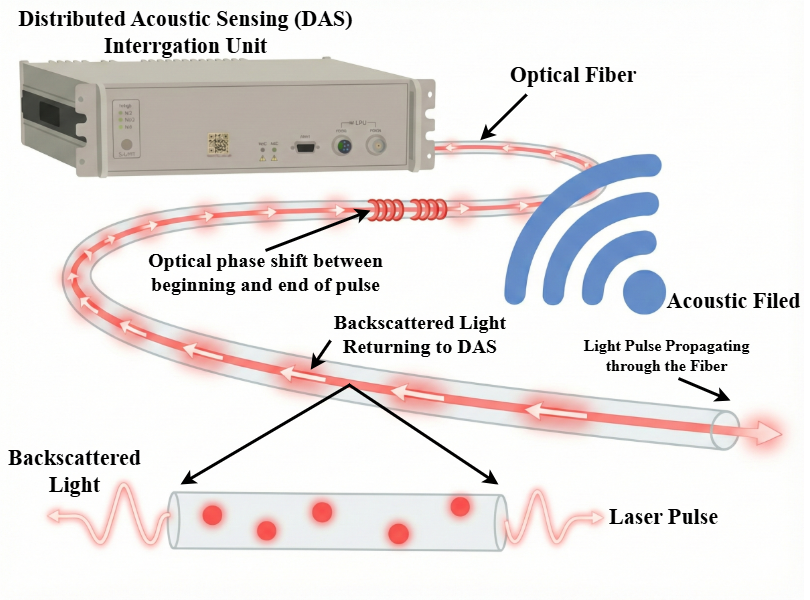
\includegraphics[width=0.85\textwidth]{Figures/fig01_DAS.png}
\caption{Distributed acoustic sensing system.}
\label{fig:das-system}
\end{figure}

For analysis, DAS measurements are commonly represented as spatio-temporal distance--time maps or as time--frequency matrices from which descriptors are derived~\cite{kandamali2022ml}. This representation underpins the multi-domain design adopted in this thesis, in which one window is described simultaneously in the time, frequency, time--frequency, and spatial domains. The breadth of DAS applications has also motivated dedicated reviews of DAS methodologies and deep-learning approaches, including in subsurface settings~\cite{shahabudin2025review}.

\subsection{DAS Signal Processing}
\label{sec:chap2DASsignal}
\autoBookmark{subsec}{DAS Signal Processing}
Raw $\Phi$-OTDR signals are high-dimensional and noisy, and front-end processing therefore aims to raise the signal-to-noise ratio, mitigate coherent fading, and convert backscatter into representations suitable for classification~\cite{kandamali2022ml}. Typical pipelines apply temporal and spatial band-pass filtering, amplitude normalisation, and channel selection or aggregation. To address the non-stationarity of footsteps, vehicles, and excavation, STFT- or wavelet-based time--frequency analysis is widely used. The choice and ordering of these operations are consequential, because any component of the raw measurement that survives preprocessing is absorbed into the descriptors as though it were information about the event.

Early long-perimeter intrusion systems combined handcrafted features such as energy, spectral amplitude, and variance with fixed thresholds and spatial-consistency checks; these systems performed adequately in controlled settings but degraded under environmental variability, which motivated adaptive, learning-based methods~\cite{juarez2005intrusion}. Learned denoising has since been proposed, for example with densely connected residual convolutional networks~\cite{huang2024noise}. The preprocessing chain in this thesis follows the same principles, combining DC-offset removal, Butterworth band-pass filtering, and z-score normalisation, with the normalisation step additionally serving as a leakage control (\refss{sec:chap3Normalisation}).

\subsection{Event Classification Using Classical Machine Learning}
\label{sec:chap2DASclassicalML}
\autoBookmark{subsec}{Classical ML for DAS}
A substantial body of work pairs handcrafted features with classical models, following the general workflow illustrated in \reff{fig:das_machine_learning}. Bublin demonstrated that knowledge-based features combined with classical ML and deep learning could exceed $99.9\%$ accuracy on binary excavator detection, using Fourier and RMS descriptors together with image-derived features~\cite{bublin2021event}, and had earlier compared classical, image-based, and deep approaches more broadly~\cite{bublin2019ml}. Cao et al.\ released an open six-class $\Phi$-OTDR dataset with SVM and CNN baselines, the SVM operating on 16 handcrafted statistical and spectral features~\cite{caoxin2023opendataset}. For urban traffic, Min et al.\ extracted vehicle signals by filtering and scaling ahead of a radial-basis-function SVM~\cite{min2024vehicle}. Shen et al.\ reduced time-domain statistics and fed them, together with a convolutional-recurrent encoder, into a gradient-boosting classifier for imbalanced fibre-vibration data~\cite{shen2024abnormal}, and Kozmin et al.\ combined wavelet packet decomposition and PCA with a hybrid logistic-regression and residual-CNN model~\cite{kozmin2025wavelet}. These studies establish that carefully engineered descriptors combined with lightweight classifiers are effective for DAS event discrimination, particularly when the number of classes is small.

\begin{figure}[!htbp]
\centering
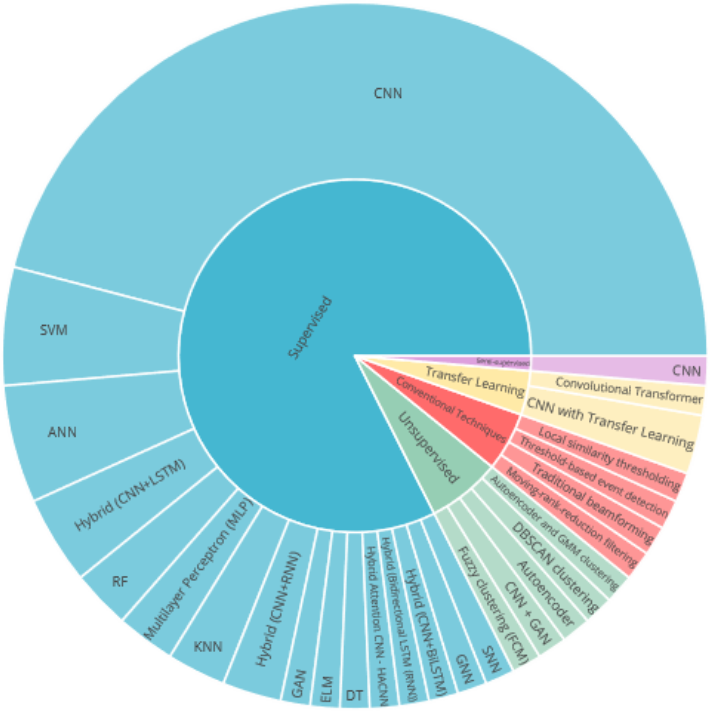
\includegraphics[width=0.68\textwidth]{Figures/fig02_ML_classification.png}
\caption{Machine learning workflow for event detection and classification \cite{shahabudin2025review}.}
\label{fig:das_machine_learning}
\end{figure}

\subsection{Event Classification Using Deep Learning and Graph Models}
\label{sec:chap2DASdeepLearning}
\autoBookmark{subsec}{Deep Learning for DAS}
More recent work applies supervised deep learning directly to DAS spectrograms or distance--time representations~\cite{tomasov2023enhancing,tomasov2025perimeter}. Convolutional long short-term memory networks have been used for temporal modelling in railway intrusion detection~\cite{li2020convlstm}, and deep models have been deployed for intrusion detection and impulsive-event classification across operational telecommunications networks~\cite{han2024intrusion}. Semi-supervised learning has been explored to reduce annotation demands, for example for rock-slope failure monitoring~\cite{kang2024semisupervised}.

Transformer and graph architectures now set the reported state of the art on the public campus benchmark used in this thesis. Dione et al.\ introduced DASViT1D, a one-dimensional vision transformer over multi-domain (MFCC, RDFT, DWT) inputs, reporting $93.5\%$ accuracy on the nine-class taxonomy~\cite{dione2025intrusion}, and later DAStatFormer, a multi-branch transformer that integrates 24 statistical features per channel, reporting $99.93\%$~\cite{dione2026dastatformer}. Jeong et al.\ proposed S2-DyGNN, a spectro-spatial dynamic graph neural network that treats the channel axis as a graph and reports $94.0\%$, alongside graph attention and graph convolutional baselines~\cite{jeong2026s2dygnn}; graph neural networks have also been applied to microseismic event detection in DAS data~\cite{shahabudin2024gnn}. A benchmark comparing convolutional, recurrent, transformer, state-space, and classical models found no single architecture best under all conditions~\cite{shi2025benchmarking}. These figures are not directly comparable with one another, because each is obtained under its own partition, window density, and taxonomy; \refs{sec:chap2RelatedWorks} records the protocol alongside each result for that reason.

\subsection{Real-Time and Deployment Considerations}
\label{sec:chap2DASdeployment}
\autoBookmark{subsec}{Real-Time and Deployment Considerations}
Recognition accuracy is necessary but insufficient for operational monitoring, which imposes constraints on latency, throughput, bandwidth, and energy consumption across sensing, transport, storage, and inference~\cite{deng2025roadtraffic}. Deep networks tailored to DAS can achieve high accuracy but often require hardware accelerators and further optimisation to satisfy deployment constraints; they also remain susceptible to dataset shift and calibration drift~\cite{shi2025benchmarking}. These considerations have motivated both efficient deep architectures and feature-engineered pipelines for which the cost of each processing stage can be quantified explicitly. Production studies of DAS road-traffic systems identify inference-pipeline design and buffered pre-computation as key engineering challenges~\cite{deng2025roadtraffic}, while hybrid ensembles have demonstrated reliable real-time hazard detection on railways~\cite{yurekli2025railway}. Few studies report the online computational cost of the complete pipeline rather than that of the classifier alone; those that provide timing data generally report only inference cost.

Lightness is therefore claimed more often than it is measured. A model may be light in one respect and heavy in another: a network with few parameters may still require many hours of GPU training, and a classifier that predicts within microseconds may depend on an input transform that dominates the processing time per window. A complete account of the footprint of a model requires four quantities: the stored size of the trained model, the per-window inference latency, the end-to-end latency including the preparation of the input, and the training time together with the hardware it requires. Only a comparison of models on all four quantities, on the same hardware, allows a claim of lightness to be verified. This thesis adopts that account (\refs{sec:ResearchBackground}) and applies it to the pipeline and to every baseline.

\subsection{Evaluation Protocols and Data Leakage}
\label{sec:chap2Leakage}
\autoBookmark{subsec}{Evaluation Protocols and Data Leakage}
Data leakage is the unintended transfer of information from evaluation data into model training, so that a model is assessed with information it could not legitimately possess at deployment~\cite{kaufman2012leakage}. It is a recognised cause of overly optimistic and irreproducible results in applied machine learning: a review of machine-learning-based science found leakage in at least 294 published studies across seventeen fields and organised it into a taxonomy whose forms include preprocessing and feature selection fitted on training and test data together, temporal leakage, and non-independence between training and test samples~\cite{kapoor2023leakage}. Three families of leakage are relevant to DAS event classification: leakage through dependent samples, leakage through the modelling pipeline, and leakage into the statistical comparison of methods. The subsections below review the controls that the literature recommends for each family, and Table~\ref{tab:leakage_controls} relates every control to its implementation in Chapter~\ref{chap:methodology}.

\begin{table}[!htbp]
	\centering
	\caption{Leakage pathways relevant to DAS event classification, the controls recommended in the literature, and their implementation in this thesis.}
	\label{tab:leakage_controls}
	\footnotesize
	\setlength{\tabcolsep}{4pt}
	\renewcommand{\arraystretch}{1.15}
	\begin{tabularx}{\textwidth}{@{}>{\raggedright\arraybackslash}p{2.3cm} >{\raggedright\arraybackslash}X >{\raggedright\arraybackslash}X >{\raggedright\arraybackslash}X@{}}
		\toprule
		\textbf{Pathway} & \textbf{Mechanism} & \textbf{Recommended control} & \textbf{Implementation in this thesis}\\
		\midrule
		Overlapping windows & Random window-level splits place near-duplicate windows in training and test & Blocked partitions with a gap between training and test blocks~\cite{burman1994hblock,racine2000hvblock,bergmeir2012timeseries,dehghani2019windows} & Blocked segments with one-window guard bands; raw-sample disjointness asserted (Sec.~\ref{sec:chap3Partitioning})\\
		\addlinespace[3pt]
		Recording or session dependence & Samples from one recording appear in both training and test & Partitioning by subject, session, or recording~\cite{saeb2017usecase,roberts2017crossvalidation} & Session-grouped (Cao) and recording-segment (Tomasov) partitions; leave-one-date-out and leave-one-recording-out evaluation (Secs.~\ref{sec:chap3Partitioning} and~\ref{sec:chap3ConfoundDesign})\\
		\addlinespace[3pt]
		Feature selection outside the training fold & Selection uses rows that are later used for evaluation & Selection repeated inside every training fold~\cite{ambroise2002selection} & Selectors fitted on training rows and refitted per fold (Sec.~\ref{sec:chap3FeatureSelection})\\
		\addlinespace[3pt]
		Model selection on evaluation data & Configurations are chosen on the data used to report performance & Separate validation data or nested cross-validation~\cite{varma2006bias,cawley2010overfitting} & Selection on the validation set; test scores reported once (Sec.~\ref{sec:chap3ModelReady})\\
		\addlinespace[3pt]
		Resampling before partitioning & Synthetic samples interpolate across the split & Resampling inside the training fold only~\cite{santos2018imbalanced} & Resamplers inside the training pipeline (Sec.~\ref{sec:chap3Balancing})\\
		\addlinespace[3pt]
		Preprocessing fitted on all data & Scaling statistics include evaluation rows & Preprocessing fitted on training data alone~\cite{kapoor2023leakage} & Stateless per-window preprocessing; scaler inside the training pipeline (Secs.~\ref{sec:chap3Preprocessing} and~\ref{sec:chap3ModelReady})\\
		\addlinespace[3pt]
		Dependent units in statistics & Tests and intervals treat dependent results as independent & Independent replicates, corrected tests, and cluster resampling~\cite{dietterich1998tests,nadeau2003inference,field2007clustered} & Repeated partitions, group bootstrap, and paired tests over held-out acquisitions (Sec.~\ref{sec:chap3Statistics})\\
		\bottomrule
	\end{tabularx}
\end{table}

\subsubsection{Leakage Through Dependent Samples}
\label{sec:chap2LeakDependent}
\autoBookmark{subsubsec}{Leakage Through Dependent Samples}
The first family arises when training and test samples are not independent. Roberts et al.~\cite{roberts2017crossvalidation} demonstrate that, for temporally, spatially, and hierarchically structured data, random cross-validation systematically overestimates predictive performance, and they recommend blocked partitions whose boundaries follow the dependence structure of the data. For serially dependent observations, h-block cross-validation removes a band of observations on either side of each test observation so that no training observation lies close to it~\cite{burman1994hblock}, hv-block cross-validation extends the idea to consistent model selection~\cite{racine2000hvblock}, and blocked schemes of this kind give more reliable error estimates for time-series predictors than random partitioning~\cite{bergmeir2012timeseries}. When several samples are drawn from one subject, the corresponding requirement is that the split be made by subject rather than by record: in clinical sensor data, record-wise cross-validation substantially overestimates the accuracy that subject-wise cross-validation measures~\cite{saeb2017usecase}. Sliding-window segmentation compounds the problem, because overlapping windows from one stream are near-duplicates, and the apparent benefit of overlapping windows in human activity recognition has been traced to evaluation schemes that do not keep the windows of one subject together~\cite{dehghani2019windows}.

These findings transfer directly to DAS. Overlapping analysis windows are serially dependent observations in the sense of h-block cross-validation, so a gap of at least one window length between training and test windows plays the role of the removed band. A recording session plays the role of the clinical subject, so the session or recording, rather than the window, is the natural unit of partitioning. The partitions of Chapter~\ref{chap:methodology} apply both principles, grouping Cao records by session and dividing each Tomasov recording into blocked segments separated by guard bands.

\subsubsection{Leakage Through the Modelling Pipeline}
\label{sec:chap2LeakPipeline}
\autoBookmark{subsubsec}{Leakage Through the Modelling Pipeline}
The second family arises when a fitted component of the pipeline is exposed to data that are later used for evaluation. Feature selection performed on the full dataset before cross-validation is the best-known case: in microarray classification it severely underestimates the error rate, and an unbiased estimate requires selection to be repeated within every training fold~\cite{ambroise2002selection}. Using cross-validation both to tune a model and to estimate its error introduces a comparable optimistic bias~\cite{varma2006bias}, and selecting among many configurations on the data used to report performance overfits the selection criterion itself~\cite{cawley2010overfitting}. Resampling for class imbalance creates a further pathway, because oversampling before partitioning places synthetic samples derived from evaluation instances in the training data and yields over-optimistic estimates~\cite{santos2018imbalanced}. The common remedy is to treat every data-dependent operation, including scaling, feature selection, and resampling, as part of the model, fitting it on training data alone and applying it unchanged to evaluation data~\cite{kapoor2023leakage}. Chapter~\ref{chap:methodology} adopts this principle throughout and also measures the bias that feature selection outside the cross-validation loop would introduce.

\subsubsection{Leakage into Statistical Comparison}
\label{sec:chap2LeakStatistics}
\autoBookmark{subsubsec}{Leakage into Statistical Comparison}
The third family concerns the statistics used to compare methods, which assume that the units over which they are computed are independent. Dietterich~\cite{dietterich1998tests} showed that several widely used tests for comparing classifiers, including the resampled paired $t$-test, have an elevated Type~I error because their samples share data, and Nadeau and Bengio~\cite{nadeau2003inference} showed that the overlap between training sets in repeated resampling causes the variance of the estimated generalisation error to be underestimated, and proposed a corrected test. For comparing several classifiers across several datasets, Dem\v{s}ar~\cite{demsar2006statistical} recommends the Friedman test with post-hoc Nemenyi analysis, with the datasets serving as independent blocks, together with step-down procedures such as Holm's for families of pairwise comparisons~\cite{holm1979simple}. Where observations are clustered, as windows are within recordings, resampling should operate on whole clusters so that bootstrap intervals reflect the dependence between observations~\cite{field2007clustered}. The statistical procedures of Chapter~\ref{chap:methodology} follow these principles by replicating over independently generated partitions and independent acquisitions rather than over configurations of a single partition.

\subsubsection{Leakage in Published DAS Benchmarks}
\label{sec:chap2LeakDAS}
\autoBookmark{subsubsec}{Leakage in Published DAS Benchmarks}
In DAS, the dependence structure that makes these controls necessary is physical rather than incidental. Overlapping analysis windows share raw interrogator samples, and all samples from a given recording session share the fibre state, coupling, interrogator configuration, and ambient conditions~\cite{tomasov2025dataset,caoxin2023opendataset}. Distributing such dependent samples across partitions enables a model to exploit recording-specific structure rather than event characteristics. The public datasets used in this thesis illustrate both mechanisms. Cao et al.~\cite{caoxin2023opendataset} release a fixed $8{:}2$ partition of $15{,}419$ pre-segmented records and report SVM and CNN baselines on it. Tomasov et al.~\cite{tomasov2025perimeter} generate classification vectors by sliding an $8{,}192$-sample window with a 256-sample stride, a $96.9\%$ overlap, and evaluate with random 10-fold cross-validation. Neither protocol constrains samples from one continuous recording to one side of the partition. Later studies adopt partial controls: Dione et al.~\cite{dione2025intrusion} fit their scaler on training folds only but do not address window or recording overlap, and Jeong et al.~\cite{jeong2026s2dygnn} use a chronological split with a five-window guard band, which removes window overlap at the boundary but still places segments of every recording on both sides. No study in Table~\ref{tab:relatedworks} groups its partition by recording, session, or acquisition date, and none reports verifying that its test set is disjoint from its training set at the level of raw measurements.

Reporting practice compounds the problem. A study that evaluates only within the campaign that produced its training data characterises performance at a site already represented in training, not at a new site. Both quantities are useful, but they answer different questions and, as Chapter~\ref{chap:ResultsAndDiscussion} shows, differ substantially in magnitude. This gap is methodological rather than algorithmic. It cannot be closed by improved features or larger models; it requires partitioning that respects the dependence structure, verification that the partition achieves what it claims, and reporting that states which protocol produced which result.

\subsubsection{Evaluation as a Software Engineering Concern}
\label{sec:chap2LeakSoftware}
\autoBookmark{subsubsec}{Evaluation as a Software Engineering Concern}
Software-engineering research on machine-learning systems offers a means of making such verification routine. Sculley et al.~\cite{sculley2015debt} describe how data dependencies and pipeline complexity accumulate as hidden technical debt that conventional code review does not reveal, and Breck et al.~\cite{breck2017mltest} respond with a rubric of concrete tests for the data, model, and infrastructure of a production system. The NeurIPS reproducibility programme applies a similar principle to research by requiring that published claims be accompanied by code and a checklist~\cite{pineau2021reproducibility}. The common principle is that a property of a machine-learning system should be tested rather than asserted. This principle has not yet been adopted in DAS event classification, where the validity of an evaluation is stated in a sentence of prose, if it is stated at all. This thesis adopts it directly by implementing its leakage controls as assertions within the pipeline (\refss{sec:chap3Partitioning}), which converts a protocol description into a property that a reader can verify.

\section{Summary of Related Works}
\label{sec:chap2RelatedWorks}
\autoBookmark{sec}{Summary of Related Works}
Table~\ref{tab:relatedworks} consolidates the most relevant prior studies, recording for each the event taxonomy, feature representation, model, reported accuracy, evaluation protocol, and whether leakage was controlled. Because the protocols, datasets, and taxonomies differ, the reported accuracies provide context rather than a ranking, and this thesis draws no comparison between them. Two observations emerge. High accuracies are most often reported for tasks with few, well-separated classes, and the strongest recent results on the nine-class campus benchmark are obtained by high-capacity transformer and graph models evaluated under random or chronological partitions of overlapping windows.

\begin{landscape}
\begin{table}[p]
\centering
\caption{Summary of related works on DAS event classification, with the evaluation protocol of each study.}
\label{tab:relatedworks}
\scriptsize
\setlength{\tabcolsep}{4pt}
\renewcommand{\arraystretch}{1.2}
\begin{tabular}{@{}>{\raggedright\arraybackslash}p{2.3cm} >{\raggedright\arraybackslash}p{2.8cm} >{\raggedright\arraybackslash}p{3.7cm} >{\raggedright\arraybackslash}p{4.2cm} >{\raggedright\arraybackslash}p{3.4cm} >{\raggedright\arraybackslash}p{3.7cm}@{}}
\toprule
\textbf{Study (Year)} & \textbf{Dataset (labels)} & \textbf{Feature representation} & \textbf{Model and reported accuracy} & \textbf{Evaluation protocol} & \textbf{Leakage control}\\
\midrule
Bublin (2021)~\cite{bublin2021event} & Own; 2 (excavator vs.\ none) & FFT; RMS windows; Sobel image features & kNN 99.96\%, RF 99.95\%, CNN 99.91\% & Random split & Not reported\\
Cao et al.\ (2023)~\cite{caoxin2023opendataset} & Cao; 6 & 16 handcrafted statistical/spectral (1D); raw time--space matrices (2D) & SVM, CNN & Random 8:2 over pre-segmented records & No; 423 of 441 sessions contribute to both folders\\
Tomasov et al.\ (2023)~\cite{tomasov2023enhancing} & Tomasov; 7 & Hann window; oversampled DFT; band-limited power (50--500\,Hz) & CNN, 91.4\% & Random 8:2 over pre-segmented records & No\\
Han et al.\ (2024)~\cite{han2024intrusion} & Own; 2 (intrusion, impulsive events) & HPF, STFT, mel spectrogram, MFCC & ConvNets, ViT, RF; 95\% & Random split & Not reported\\
Min et al.\ (2024)~\cite{min2024vehicle} & Own; 2 (vehicle vs.\ noise) & Low-pass, FK/FX/dip filters, scaling & SVM (RBF); 80\% & Random split & Not reported\\
Shen et al.\ (2024)~\cite{shen2024abnormal} & Own; 2 (human vs.\ natural) & 16-D time statistics reduced to 6-D & ConvLSTM encoder + XGBoost; 99.1\% & Random split & Not reported\\
Kozmin et al.\ (2025)~\cite{kozmin2025wavelet} & Own; 3 (digging, footsteps, noise) & WPD features; PCA & Logistic regression + ResNet CNN; 98\% & Random split & Not reported\\
Shi \& Zong (2025)~\cite{shi2025benchmarking} & Own; 4 & CSDM phase maps; VAE compression & ResNet 95.8\%, MLP 95.3\%, others & Random split & Not reported\\
Tomasov et al.\ (2025)~\cite{tomasov2025perimeter} & Tomasov; 9 & FFT, RDFT, DWT, MFCC & 1D CNN, XGBoost; MFCC 85.61\%, RDFT 85.47\% & Random 10-fold CV, 80/10/10, 8{,}192-sample windows at 256-sample stride (96.9\% overlap) & No; 100\% of test windows share raw samples with training (\refs{sec:resLeakage})\\
Dione et al.\ (2025)~\cite{dione2025intrusion} & Tomasov; 9. Cao; 6 & Multi-domain fusion (MFCC, RDFT, DWT) & DASViT1D; 93.5\% & Fixed 80/10/10 into ``non-overlapping subsets'' & Partial; scaler fitted on training folds only, window and recording overlap not addressed\\
Jeong et al.\ (2026)~\cite{jeong2026s2dygnn} & Tomasov; 9. Cao; 6 & STFT spectrograms; 2D frequency--time CNN features & S2-DyGNN; 94.0\% (GAT 81.2\%, GCN 85.3\%) & Chronological 80/10/10 with a 5-window guard band & Windows yes, recordings no; split is chronological within the stream, not grouped by recording\\
Dione et al.\ (2026)~\cite{dione2026dastatformer} & Tomasov; 9. Cao; 6 & 24 analysis-of-variance statistical features per channel & DAStatFormer; 99.93\% (Tomasov), 99.48\% (Cao) & Stratified random 80/20 per class & No; no grouping by recording\\
\midrule
\textbf{This study} & Tomasov; 9 (primary). Cao; 6 (evaluation) & 1{,}002 multi-domain features (time 112, frequency 90, time--frequency 739, spatial 61) & LightGBM (proposed); XGBoost, LR, and others; CNN, GNN, and transformer baselines on identical partitions & Blocked segments with guard bands (Tomasov); session-grouped (Cao) & Yes; verified programmatically before training\\
\bottomrule
\end{tabular}
\end{table}
\end{landscape}

Table~\ref{tab:feature-domain-coverage} compares the feature-domain coverage of these studies. A check mark indicates that the study explicitly uses an input representation or engineered descriptor from that domain; for the spatial column, only methods that retain or derive information across DAS channels or from a space--time representation are counted. No prior study covers all four domains: eleven of the twelve combine two or three, and only Han et al.~\cite{han2024intrusion} pair time-domain descriptors with both time--frequency and spatial information. The complementarity of the four domains has therefore not been tested on these benchmarks, which motivates RQ2.

\begin{table}[H]
\centering
\caption{Feature-domain coverage in related DAS event-classification studies.}
\label{tab:feature-domain-coverage}
\footnotesize
\setlength{\tabcolsep}{4pt}
\renewcommand{\arraystretch}{1.25}
\begin{tabular}{@{}>{\raggedright\arraybackslash}p{4.0cm} >{\centering\arraybackslash}p{1.8cm} >{\centering\arraybackslash}p{2.1cm} >{\centering\arraybackslash}p{2.4cm} >{\centering\arraybackslash}p{3.0cm}@{}}
\toprule
\textbf{Author (Year)} & \textbf{Time domain} & \textbf{Frequency domain} & \textbf{Time--frequency domain} & \textbf{Spatial/spatio-temporal domain}\\
\midrule
Bublin (2021)~\cite{bublin2021event} & $\checkmark$ & $\checkmark$ & $\times$ & $\checkmark$\\
Cao et al.\ (2023)~\cite{caoxin2023opendataset} & $\checkmark$ & $\checkmark$ & $\times$ & $\checkmark$\\
Tomasov et al.\ (2023)~\cite{tomasov2023enhancing} & $\times$ & $\checkmark$ & $\times$ & $\times$\\
Han et al.\ (2024)~\cite{han2024intrusion} & $\checkmark$ & $\times$ & $\checkmark$ & $\checkmark$\\
Min et al.\ (2024)~\cite{min2024vehicle} & $\checkmark$ & $\checkmark$ & $\times$ & $\checkmark$\\
Shen et al.\ (2024)~\cite{shen2024abnormal} & $\checkmark$ & $\times$ & $\times$ & $\checkmark$\\
Kozmin et al.\ (2025)~\cite{kozmin2025wavelet} & $\times$ & $\times$ & $\checkmark$ & $\checkmark$\\
Shi \& Zong (2025)~\cite{shi2025benchmarking} & $\times$ & $\checkmark$ & $\times$ & $\checkmark$\\
Tomasov et al.\ (2025)~\cite{tomasov2025perimeter} & $\times$ & $\checkmark$ & $\checkmark$ & $\times$\\
Dione et al.\ (2025)~\cite{dione2025intrusion} & $\times$ & $\checkmark$ & $\checkmark$ & $\times$\\
Jeong et al.\ (2026)~\cite{jeong2026s2dygnn} & $\times$ & $\times$ & $\checkmark$ & $\checkmark$\\
Dione et al.\ (2026)~\cite{dione2026dastatformer} & $\checkmark$ & $\times$ & $\times$ & $\checkmark$\\
\midrule
\textbf{Proposed pipeline} & $\checkmark$ & $\checkmark$ & $\checkmark$ & $\checkmark$\\
\bottomrule
\end{tabular}
\end{table}

\section{Research Gap}
\label{sec:chap2ResearchGap}
\autoBookmark{sec}{Research Gap}
The review identifies three research gaps, each of which motivates one research question.

The first gap concerns the computational footprint of DAS classifiers (RQ1). The strongest recent results are obtained by high-capacity transformer and graph models whose computational demands and limited interpretability are poorly matched to the resource-constrained, audit-sensitive requirements of perimeter security. Where the reviewed studies report computational cost, they report the inference time of the classifier (\refss{sec:chap2DASdeployment}); the stored model size, the training time and hardware, and the cost of preparing the input are rarely given, and seldom for several models on the same embedded platform. The properties that make a DAS classifier lightweight have therefore been asserted rather than measured, and a lightweight alternative to the recent architectures has no defined target to satisfy.

The second gap concerns representation (RQ2). Individual feature domains have been studied extensively, but no prior study covers all four (Table~\ref{tab:feature-domain-coverage}), and systematic comparisons of multi-domain fusion with single domains, of consensus feature selection, and of class balancing remain scarce, particularly on more than one acquisition system. Nor has feature selection been assessed for its effect on the footprint of a model as well as on its accuracy.

The third gap concerns evaluation (RQ3). The general literature on leakage prescribes controls for dependent samples, for pipeline fitting, and for statistical comparison (\refss{sec:chap2Leakage}), and in DAS data the dependence that makes these controls necessary is physical. Yet no study in Table~\ref{tab:relatedworks} groups its partition by recording, session, or acquisition date; only one separates training and test windows with a guard band; and none verifies disjointness at the level of raw measurements. Because protocol leakage confounds the merit of a model with the leniency of its partition, published figures cannot be compared with one another, and a new pipeline cannot be assessed fairly until its own evaluation has been shown to be free of leakage. Chapter~\ref{chap:ResultsAndDiscussion} confirms the problem in both benchmarks used in this thesis. The recent architectures have likewise not been compared with lightweight feature pipelines on identical partitions under a single protocol, and none of the reviewed studies tests whether a fitted model generalises to unseen recordings, acquisition campaigns, or a second sensing system.

Table~\ref{tab:position} expresses the gaps as properties that can be counted across the twelve studies of Table~\ref{tab:relatedworks}, and it indicates where the novelty of this thesis lies: most of these properties are entirely absent from the reviewed work. The first gap is not included in the table, because the reviewed papers report cost too inconsistently to be tabulated property by property; \refs{sec:resEfficiency} measures it directly instead.

\begin{table}[!htbp]
	\centering
	\caption{Properties of the twelve reviewed studies, by research gap, compared with this thesis.}
	\label{tab:position}
	\footnotesize
	\setlength{\tabcolsep}{4pt}
	\renewcommand{\arraystretch}{1.2}
	\begin{tabularx}{\textwidth}{@{}l >{\raggedright\arraybackslash}X >{\centering\arraybackslash}p{1.5cm} >{\raggedright\arraybackslash}p{5.0cm}@{}}
		\toprule
		\textbf{Gap} & \textbf{Property} & \textbf{Studies with it} & \textbf{This thesis}\\
		\midrule
		RQ2 & Descriptors from all four feature domains & 0 of 12 & Yes\\
		RQ2 & Selection by consensus across selector families & 0 of 12 & Yes, eight selectors\\
		\addlinespace[3pt]
		RQ3 & Partition grouped by recording, session, or date & 0 of 12 & Yes: session (Cao) and recording segment (Tomasov), with hold-out of whole acquisitions\\
		RQ3 & Guard band between training and test windows & 1 of 12 & Yes\\
		RQ3 & Disjointness verified at the level of raw measurements & 0 of 12 & Yes, asserted in code\\
		RQ3 & Effect of the protocol isolated by changing only the partition & 0 of 12 & Yes, for a CNN, five architectures, and the pipeline\\
		RQ3 & Evaluation on more than one sensing system & 3 of 12 & Yes\\
		RQ3 & Fitted model tested on a second sensing system & 0 of 12 & Yes, in both directions\\
		\bottomrule
	\end{tabularx}
\end{table}

This thesis addresses the three gaps in turn. It defines a lightweight classifier by four measured quantities, namely model size, inference latency, end-to-end latency, and training cost, and measures them for the pipeline and for every baseline on a single embedded platform (RQ1). It develops a feature-driven pipeline that combines multi-domain descriptors, consensus selection, and class balancing with classifiers that train and predict on CPU cores, and it measures the contribution of each component (RQ2). It then establishes verified group-aware partitions as its evaluation basis, measures the effect of the protocol by varying only the partition, compares the pipeline with the CNN published with each dataset and with five recent architectures, and tests the extent to which its performance generalises beyond the recordings and the sensing system on which it was trained (RQ3). No claim of superiority over the studies in Table~\ref{tab:relatedworks} under their own protocols is made.

\section{Chapter Summary}
\label{sec:chap2Summary}
\autoBookmark{sec}{Chapter Summary}
This chapter reviewed the literature relevant to feature-driven DAS event classification, including the leakage controls that valid evaluation requires (Table~\ref{tab:leakage_controls}). The synthesis of prior studies (Table~\ref{tab:relatedworks}) revealed three gaps: the footprint that makes a DAS classifier lightweight has been claimed rather than measured; four-domain fusion, consensus selection, and class balancing have not been evaluated systematically; and no published protocol on these benchmarks has been verified to be free of leakage, so that lightweight feature pipelines have been neither compared with recent architectures nor tested for generalisation beyond their training recordings under a single verified protocol. The review also established the distinction between white-box and black-box models, to which the discussion of Chapter~\ref{chap:ResultsAndDiscussion} returns. Chapter~\ref{chap:methodology} describes the methodology developed to address these gaps.


%Chapter 3
\pagestyle{plain}\cleardoublepage %To add an empty page and start on an odd number (SOFTBOUND)%%
\chapter{METHODOLOGY}\label{chap:methodology}
\autoBookmark{chap}{METHODOLOGY}
\section{Overview}%
\label{sec:chap3Overview}
\autoBookmark{sec}{Overview}
This chapter describes how the DAS event-classification artefact was designed, built, demonstrated, and evaluated. The artefact is a feature-driven pipeline that turns a raw DAS window into an event label through window-level conditioning, multi-domain feature engineering, ensemble feature selection, class-imbalance treatment, and lightweight classification. Every learning component runs on CPU cores, and the footprint of the whole pipeline, model size, latency, and training cost, is measured on the embedded platform on which it is meant to run. Its evaluation protocol is treated as part of the artefact rather than as neutral context: an accuracy that a deployment could not reproduce does not meet the design objectives, however good the individual components are.

The pipeline was designed on the Tomasov perimeter-security dataset, the primary dataset of the thesis, and then applied without modification to the Cao dataset, which serves as an independent evaluation dataset. Both datasets pass through every stage described below with the same settings. Where a stage has to treat them differently because their data are structured differently, the chapter says so explicitly.

The research follows the Design Science Research Methodology (DSRM) of Peffers et al.~\cite{peffers2007dsrm}. \refs{sec:chap3DSRMFramework} justifies that choice, presents the activity flow (\reff{fig:dsrm_flow}), and maps each research question and objective to a DSRM activity (Table~\ref{tab:dsrm_mapping}). \refs{sec:chap3DSRMProblem} to \refs{sec:chap3DSRMCommunication} then take the six activities in turn. Activity~3, the largest, contains the technical design: the datasets and how their samples are defined, the leakage found in their released protocols, the group-aware partitions that replace them, signal preprocessing, the extraction and fusion of $1{,}002$ features, the preparation of model-ready data, consensus feature selection and class balancing, classifier configuration, and the baseline models. Activity~4 describes the demonstration setting and the realised partitions. Activity~5 defines the metrics, the diagnostics, the statistical procedures, the generalisation tests, and the efficiency and lightweight-footprint measurements, and Activity~6 states how the results are communicated.

\section{Research Design: The DSRM Framework}
\label{sec:chap3DSRMFramework}
\autoBookmark{sec}{Research Design: The DSRM Framework}

\subsection{Rationale for Adopting DSRM}
\label{sec:chap3DSRMRationale}
\autoBookmark{subsec}{Rationale for Adopting DSRM}
Design science research produces and evaluates purposeful artefacts that address identified organisational or technical problems~\cite{hevner2004design}. Peffers et al.~\cite{peffers2007dsrm} operationalise this approach as a six-activity process with four possible entry points, and Gregor and Hevner~\cite{gregor2013positioning} classify the resulting knowledge contribution by the novelty of the problem and of the solution. DSRM suits the present study for three reasons. First, its principal output is a constructed artefact, a classification pipeline together with the protocol under which it is evaluated, rather than a description or explanation of a phenomenon. Second, the study is problem-centred: it starts from the operational limitations of DAS event classification (\refs{sec:ResearchProblemStatement}) and from a measurable deficiency in prevailing evaluation practice, and proceeds through design objectives and construction to assessment. Third, DSRM demands rigorous evaluation and the communication of reusable knowledge. Both demands are central here, because the most durable findings of the study concern how DAS benchmarks should be evaluated rather than which classifier wins on one of them. In Gregor and Hevner's terms, the evaluation protocol is an exaptation, known solutions carried into a field that had not applied them, and the pipeline with its diagnostics is an improvement, a new solution to a known problem (\refs{sec:chap5Contributions}).

DSRM has been applied to comparable machine-learning artefacts in engineering and information-systems research, where the artefact is a data pipeline or predictive system whose utility is established empirically. Its activities align with the three research questions of \refs{sec:ResearchQuestions}: RQ1 analyses the footprint a lightweight classifier must meet and so shapes the problem and the objectives; RQ2 guides the design and development of the pipeline and its components; and RQ3 evaluates it under a verified leakage-controlled protocol, benchmarks it against alternatives, and tests how far its performance generalises.

\subsection{DSRM Activity Flow}
\label{sec:chap3DSRMFlow}
\autoBookmark{subsec}{DSRM Activity Flow}
\reff{fig:dsrm_flow} shows the six activities as executed in this study, with the entry point, the input each activity received, the output it produced, and the section in which it is documented. The process was iterative, as Peffers et al.\ anticipate, and evidence from Activity~5 fed back into Activity~3 on three occasions. The first blocked partition of the Tomasov data balanced zone counts rather than window mass, left one class with no test samples, and was redesigned. The Friedman analysis first used to compare classifiers was withdrawn once its blocking assumption was found to be violated, and was replaced by tests over independent acquisitions. The set of baselines was widened from the two published CNNs to five architectures published from 2024 onwards. Every refinement was decided on training and validation evidence; the held-out test sets were not consulted until the final evaluation.

\begin{figure}[!htbp]
\centering
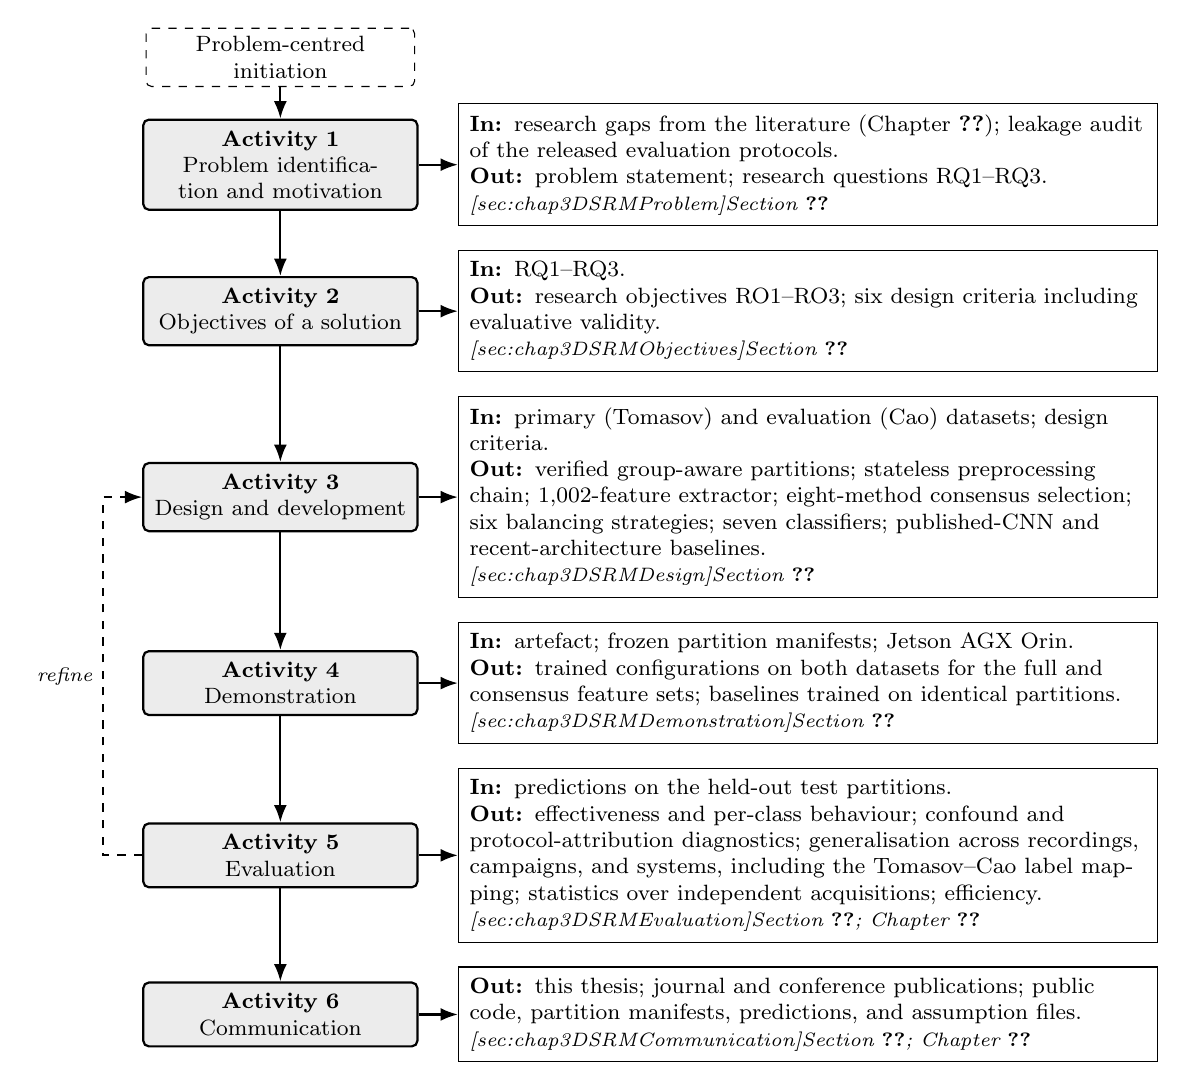
\begin{tikzpicture}[
	font=\footnotesize,
	node distance=3mm and 5mm,
	act/.style={draw, thick, rounded corners=2pt, fill=gray!15, text width=3.2cm, align=center, inner sep=4pt},
	io/.style={draw, fill=white, text width=8.6cm, align=left, inner sep=4pt},
	ref/.style={font=\scriptsize\itshape},
	arr/.style={-{Latex[length=2.2mm]}, thick},
	iter/.style={-{Latex[length=2.2mm]}, thick, dashed},
]
\node[io] (o1) {\textbf{In:} research gaps from the literature (Chapter~\ref{chap:LR}); leakage audit of the released evaluation protocols.\\\textbf{Out:} problem statement; research questions RQ1--RQ3.\\{\scriptsize\itshape \refs{sec:chap3DSRMProblem}}};
\node[io, below=of o1] (o2) {\textbf{In:} RQ1--RQ3.\\\textbf{Out:} research objectives RO1--RO3; six design criteria including evaluative validity.\\{\scriptsize\itshape \refs{sec:chap3DSRMObjectives}}};
\node[io, below=of o2] (o3) {\textbf{In:} primary (Tomasov) and evaluation (Cao) datasets; design criteria.\\\textbf{Out:} verified group-aware partitions; stateless preprocessing chain; $1{,}002$-feature extractor; eight-method consensus selection; six balancing strategies; seven classifiers; published-CNN and recent-architecture baselines.\\{\scriptsize\itshape \refs{sec:chap3DSRMDesign}}};
\node[io, below=of o3] (o4) {\textbf{In:} artefact; frozen partition manifests; Jetson AGX Orin.\\\textbf{Out:} trained configurations on both datasets for the full and consensus feature sets; baselines trained on identical partitions.\\{\scriptsize\itshape \refs{sec:chap3DSRMDemonstration}}};
\node[io, below=of o4] (o5) {\textbf{In:} predictions on the held-out test partitions.\\\textbf{Out:} effectiveness and per-class behaviour; confound and protocol-attribution diagnostics; generalisation across recordings, campaigns, and systems, including the Tomasov--Cao label mapping; statistics over independent acquisitions; efficiency.\\{\scriptsize\itshape \refs{sec:chap3DSRMEvaluation}; Chapter~\ref{chap:ResultsAndDiscussion}}};
\node[io, below=of o5] (o6) {\textbf{Out:} this thesis; journal and conference publications; public code, partition manifests, predictions, and assumption files.\\{\scriptsize\itshape \refs{sec:chap3DSRMCommunication}; Chapter~\ref{chap:Conclusion}}};

\node[act, left=of o1] (a1) {\textbf{Activity 1}\\Problem identification and motivation};
\node[act, left=of o2] (a2) {\textbf{Activity 2}\\Objectives of a solution};
\node[act, left=of o3] (a3) {\textbf{Activity 3}\\Design and development};
\node[act, left=of o4] (a4) {\textbf{Activity 4}\\Demonstration};
\node[act, left=of o5] (a5) {\textbf{Activity 5}\\Evaluation};
\node[act, left=of o6] (a6) {\textbf{Activity 6}\\Communication};
\node[draw, dashed, rounded corners=2pt, above=4mm of a1, text width=3.2cm, align=center, inner sep=3pt] (entry) {Problem-centred initiation};

\draw[arr] (entry) -- (a1);
\draw[arr] (a1) -- (a2);
\draw[arr] (a2) -- (a3);
\draw[arr] (a3) -- (a4);
\draw[arr] (a4) -- (a5);
\draw[arr] (a5) -- (a6);
\foreach \i in {1,...,6} {\draw[arr] (a\i) -- (o\i);}
\draw[iter] (a5.west) -- ++(-0.5,0) |- node[pos=0.25, left, ref] {refine} (a3.west);
\end{tikzpicture}
\caption{DSRM activity flow followed in this study, adapted from Peffers et al.~\cite{peffers2007dsrm}. Each activity lists its principal inputs and outputs and the section in which it is reported. The dashed return path marks the design refinements triggered by evaluation evidence.}
\label{fig:dsrm_flow}
\end{figure}

\subsection{Mapping of Research Questions, Objectives, and Activities}
\label{sec:chap3DSRMMapping}
\autoBookmark{subsec}{Mapping of Research Questions, Objectives, and Activities}
Table~\ref{tab:dsrm_mapping} maps each research question to its objective and DSRM activities. It is the contract against which Chapter~\ref{chap:Conclusion} judges whether each objective was met. RO1 is analytical: it draws on the review of Chapter~\ref{chap:LR} to set the lightweight requirement in Activities~1 and~2, and on the footprint measurements of Activity~5 to check it. RO2 is constructive and is met by the artefact built in Activity~3 and run in Activity~4. RO3 is evaluative. It includes the design of the leakage-controlled partitions in Activity~3, since a protocol that has not been verified cannot support an evaluation.

\begin{table}[!htbp]
\centering
\caption{Mapping of research questions, research objectives, and DSRM activities.}
\label{tab:dsrm_mapping}
\footnotesize
\setlength{\tabcolsep}{4pt}
\renewcommand{\arraystretch}{1.2}
\begin{tabularx}{\textwidth}{@{}>{\raggedright\arraybackslash}X >{\raggedright\arraybackslash}X >{\raggedright\arraybackslash}p{2.4cm}@{}}
\toprule
\textbf{Research question} & \textbf{Research objective} & \textbf{DSRM activity}\\
\midrule
\textbf{RQ1.} What computational footprint do current approaches to event classification in DAS data carry, and what makes a classification pipeline lightweight? &
\textbf{RO1.} To analyse the computational footprint of event classification in Distributed Acoustic Sensing data and establish what makes a classification pipeline lightweight. &
1 (problem), 2 (objectives), 5 (evaluation)\\
\addlinespace
\textbf{RQ2.} How can multi-domain fusion, consensus feature selection, and class balancing be combined into a lightweight pipeline for event classification in DAS data? &
\textbf{RO2.} To develop a multi-domain machine learning pipeline for event classification in Distributed Acoustic Sensing data. &
3 (design), 4 (demonstration)\\
\addlinespace
\textbf{RQ3.} How does the pipeline compare with published deep-learning baselines on identical leakage-controlled partitions in classification performance, computational cost, and generalisation? &
\textbf{RO3.} To evaluate the multi-domain machine learning pipeline for event classification in Distributed Acoustic Sensing data. &
3 (design), 4 (demonstration), 5 (evaluation)\\
\bottomrule
\end{tabularx}
\end{table}

\section{DSRM Activity 1: Problem Identification and Motivation}
\label{sec:chap3DSRMProblem}
\autoBookmark{sec}{DSRM Activity 1: Problem Identification and Motivation}
The first activity establishes the practical problem that the artefact must solve. \refs{sec:ResearchProblemStatement} set out the established difficulties: raw DAS streams are noisy and high-dimensional, engineered feature sets are redundant and costly to compute, class imbalance is severe, and the deep models that lead on accuracy are expensive to run on edge hardware. These difficulties defined the initial aim of the research, a feature-driven pipeline that is accurate, interpretable, and cheap enough to run alongside the interrogator. Analysing what ``cheap enough'' means (RO1) showed that the literature offers no common measure of it: where cost is reported it is usually an inference time, which says nothing about how large the model is, what hardware trains it, or how long its input takes to prepare (\refs{sec:chap2ResearchGap}). The lightweight requirement therefore had to be defined before it could be designed for.

A further problem emerged as the work progressed. The pipeline was first evaluated on the Tomasov dataset alone, and extending it to the Cao dataset required its evaluation protocol to be specified for data with a different structure. Doing so showed that the protocols used with both datasets allow information to pass between training and test data. The mechanism is structural. DAS event datasets are built by sliding a window along a continuous stream, so neighbouring windows share raw samples whenever the hop is shorter than the window, and every window from one recording session shares the fibre state, coupling, interrogator settings, weather, and often the operator. A partition that ignores this dependence measures how well a model recognises a recording it has already seen, which is not the quantity that matters in deployment. \refss{sec:chap3LeakageAudit} describes how the problem was identified and shows that it is real: 423 of 441 Cao sessions span the released partition, and every test window of a random Tomasov split shares raw samples with a training window. Because a published accuracy obtained under such a protocol mixes the method with the protocol, verified leakage-controlled partitions became part of the artefact and the evaluation basis for all three research questions.

\section{DSRM Activity 2: Objectives of a Solution}
\label{sec:chap3DSRMObjectives}
\autoBookmark{sec}{DSRM Activity 2: Objectives of a Solution}
The second activity translates the problem into objectives. In line with RO1 to RO3 (\refs{sec:ResearchObjectives}), the artefact must (i) meet a lightweight footprint defined by measured quantities, (ii) classify DAS events interpretably through multi-domain fusion, consensus selection, and class balancing whose effects are exposed, and (iii) withstand comparison with published baselines on identical, verified leakage-controlled partitions.

Six design criteria follow from these objectives. \emph{Effectiveness} is measured by macro-$F_1$ and balanced accuracy on held-out data. \emph{Lightweight footprint} is measured by four quantities on embedded hardware: the stored size of the trained model, per-window inference latency, per-window end-to-end latency including feature extraction, and training time together with the hardware it needs. The target is CPU-only training and inference, a model of a few megabytes, sub-millisecond classification, and an online cost that fits the window-arrival interval on a few CPU cores. Of the remaining criteria, \emph{interpretability} is measured by the traceability of every selected feature to a named descriptor and signal domain; \emph{robustness} by stability under class imbalance, repeated partitioning, and held-out acquisitions; and \emph{reproducibility} by fixed seeds, frozen partition manifests, and released code. The sixth criterion, \emph{evaluative validity}, is the property that a reported metric is measured under conditions a deployment could reproduce. It is the criterion that distinguishes this design cycle from earlier work on the same benchmarks, and it is enforced by assertions in code rather than by statements in text.

\section{DSRM Activity 3: Design and Development}
\label{sec:chap3DSRMDesign}
\autoBookmark{sec}{DSRM Activity 3: Design and Development}
The artefact is an end-to-end, feature-driven pipeline built in six phases, each documented in its own subsection: data acquisition, leakage identification, and partitioning (\refss{sec:chap3Phase1}); signal preprocessing (\refss{sec:chap3Preprocessing}); multi-domain feature extraction and fusion (\refss{sec:chap3Phase2}); preparation of model-ready data (\refss{sec:chap3ModelReady}); feature selection and class balancing (\refss{sec:chap3Phase3}); and classifier design (\refss{sec:chap3Phase4}). The baselines against which the artefact is compared, two published CNNs and five recent architectures, are described in \refss{sec:chap3Baselines}. \reff{fig:methodology_framework} draws the complete workflow as a flowchart with standard symbols, from the two datasets through partitioning, the feature pipeline, and the baseline branch to evaluation. Every phase runs on the primary Tomasov dataset and then, unchanged, on the Cao evaluation dataset; the few steps that must differ between them are marked in the figure. Its two decision points mark where the workflow branches or loops: a partition that fails verification is redesigned, and models are trained both with and without feature selection, with the validation set guiding the choice of balancing strategy, classifier, and hyperparameters. The order of the workflow is itself a control: the leakage audit and the group-aware partition come first, before any signal is processed, and every component that learns from data (feature selection, resampling, and feature scaling) is fitted on training rows only.

\clearpage
\begin{figure}[p]
\centering
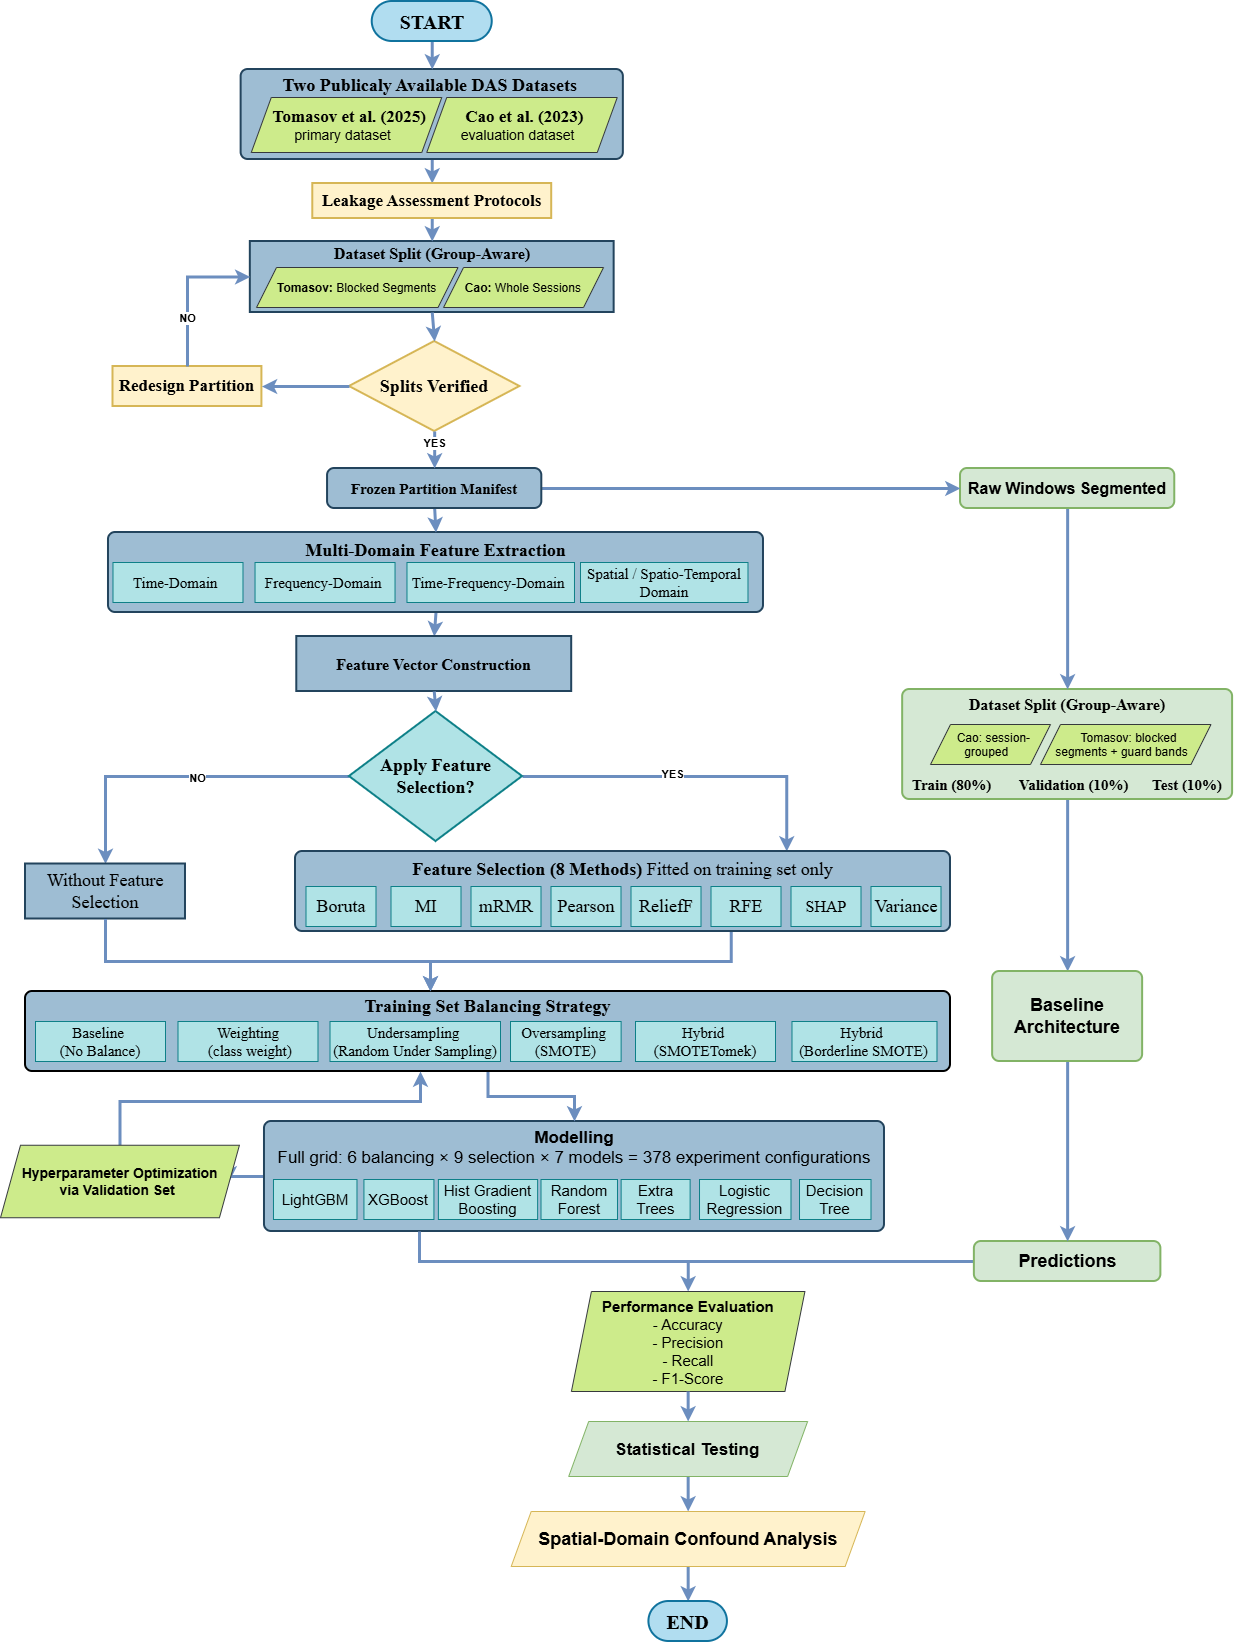
\includegraphics[width=\textwidth,height=0.80\textheight,keepaspectratio]{Figures/fig03_EC_pineline.png}
\caption[Complete workflow of the study]{Complete workflow of the study. Tomasov (primary) and Cao (evaluation) pass through the same pipeline; the branch on the right trains the baseline architectures on raw windows from the same group-aware partitions.}
\label{fig:methodology_framework}
\end{figure}
\clearpage

\subsection{Data Acquisition, Leakage Identification, and Partitioning}
\label{sec:chap3Phase1}
\autoBookmark{subsec}{Data Acquisition, Leakage Identification, and Partitioning}

\subsubsection{Dataset Description}
\label{sec:chap3Dataset}
\autoBookmark{subsubsec}{Dataset Description}
Two public DAS datasets are used, with distinct roles. The Tomasov perimeter-security dataset~\cite{tomasov2025dataset} is the primary dataset: the pipeline was designed on it, and it carries the main results. The Cao dataset~\cite{caoxin2023opendataset} is the evaluation dataset, used to test whether the design and its conclusions hold on an independent acquisition system. The two share no hardware, sensing principle, channel geometry, or event taxonomy, and that is the point of using both: a conclusion that holds on each can be attributed to the method rather than to one installation. They also arrive in different forms. Tomasov is released as continuous interrogator streams with hand-drawn annotations and no partition, whereas Cao is released as pre-segmented records already divided into fixed training and test folders. This difference governs how each is turned into labelled samples (\refss{sec:chap3Manifests}) and how its dependence structure must be controlled (\refss{sec:chap3Partitioning}). Table~\ref{tab:dataset_comparison} summarises both.

\begin{table}[!htbp]
	\centering
	\caption{The two public DAS datasets used in this study.}
	\label{tab:dataset_comparison}
	\small
	\begin{tabular}{@{}lll@{}}
		\toprule
		\textbf{Property} & \textbf{Tomasov \etal\ 2025} & \textbf{Cao \etal\ 2023}\\
		\midrule
		Role in this study  & Primary dataset            & Evaluation dataset \\
		Sensing principle   & Phase-sensitive OTDR       & Intensity $\Phi$-OTDR \\
		Interrogator        & OptaSense ODH-F            & Not specified \\
		Event classes       & 9                          & 6 \\
		Spatial channels    & 1{,}700                    & 12 \\
		Channel spacing     & 1.02\,m                    & 10\,m \\
		Sampling rate       & 20\,kHz                    & 8--12.5\,kHz (nominal) \\
		Sample unit         & Continuous stream          & Pre-segmented record \\
		Analysis windows    & 439{,}754                  & 15{,}418 \\
		Independent groups  & 16 recordings              & 441 sessions \\
		Imbalance (max:min) & 30.9:1                     & 1.3:1 \\
		\bottomrule
	\end{tabular}
\end{table}

\paragraph[Tomasov \etal\ (2025): Primary Dataset]{Tomasov \etal\ (2025): Primary Dataset.}
The perimeter-security dataset~\cite{tomasov2025dataset} was acquired with an OptaSense ODH-F interrogator on a university campus, with the fibre buried about 1\,m beneath the pavement, and is released as HDF5 files. The interrogator samples $1{,}700$ loci at 1.02\,m spacing with a 20\,kHz pulse rate. Nine event classes were annotated by hand on band-limited power maps and distributed as a Boolean mask over (time-block, locus) cells. Applying the published $8{,}192$-sample window with a $2{,}048$-sample hop yields $439{,}754$ annotated windows across 16 recordings. \reff{fig:campus_map} shows the campus layout and label points, and Table~\ref{tab:dataset} and \reff{fig:tomasov_counts} give the class-wise statistics.

\paragraph[Cao \etal\ (2023): Evaluation Dataset]{Cao \etal\ (2023): Evaluation Dataset.}
The intensity-based $\Phi$-OTDR release~\cite{caoxin2023opendataset} contains six event classes as $15{,}419$ pre-segmented MATLAB records of $10{,}000$ time samples across 12 adjacent spatial points at 10\,m spacing. Two fibre spans (5.1\,km and 10.1\,km) were used, so the same $10{,}000$ samples cover either 0.8\,s or 1.25\,s; the release carries no per-file marker distinguishing them, so a nominal sampling rate is adopted and recorded as an assumption. One zero-byte record in the released test folder, belonging to the background class, is excluded, leaving $15{,}418$ usable records: background $2{,}945$, digging $2{,}512$, knocking $2{,}530$, watering $2{,}253$, shaking $2{,}728$, and walking $2{,}450$.

\begin{table}[!htbp]
	\centering
	\caption{Class-wise statistics of the Tomasov perimeter-security dataset.}
	\label{tab:dataset}
	\small
	\begin{tabular}{@{}lrrr@{}}
		\toprule
		\textbf{Class} & \textbf{Windows} & \textbf{Recordings} & \textbf{Share (\%)}\\
		\midrule
		Regular      & 210{,}023 & 1 & 47.76\\
		Car          & 58{,}017  & 4 & 13.19\\
		Construction & 54{,}832  & 1 & 12.47\\
		Fence        & 43{,}981  & 3 & 10.00\\
		Walk         & 19{,}155  & 2 & 4.36\\
		Manipulation & 17{,}710  & 1 & 4.03\\
		Longboard    & 15{,}367  & 2 & 3.49\\
		Running      & 13{,}877  & 1 & 3.16\\
		Openclose    & 6{,}792   & 1 & 1.54\\
		\bottomrule
	\end{tabular}
\end{table}

\begin{figure}[!htbp]
\centering
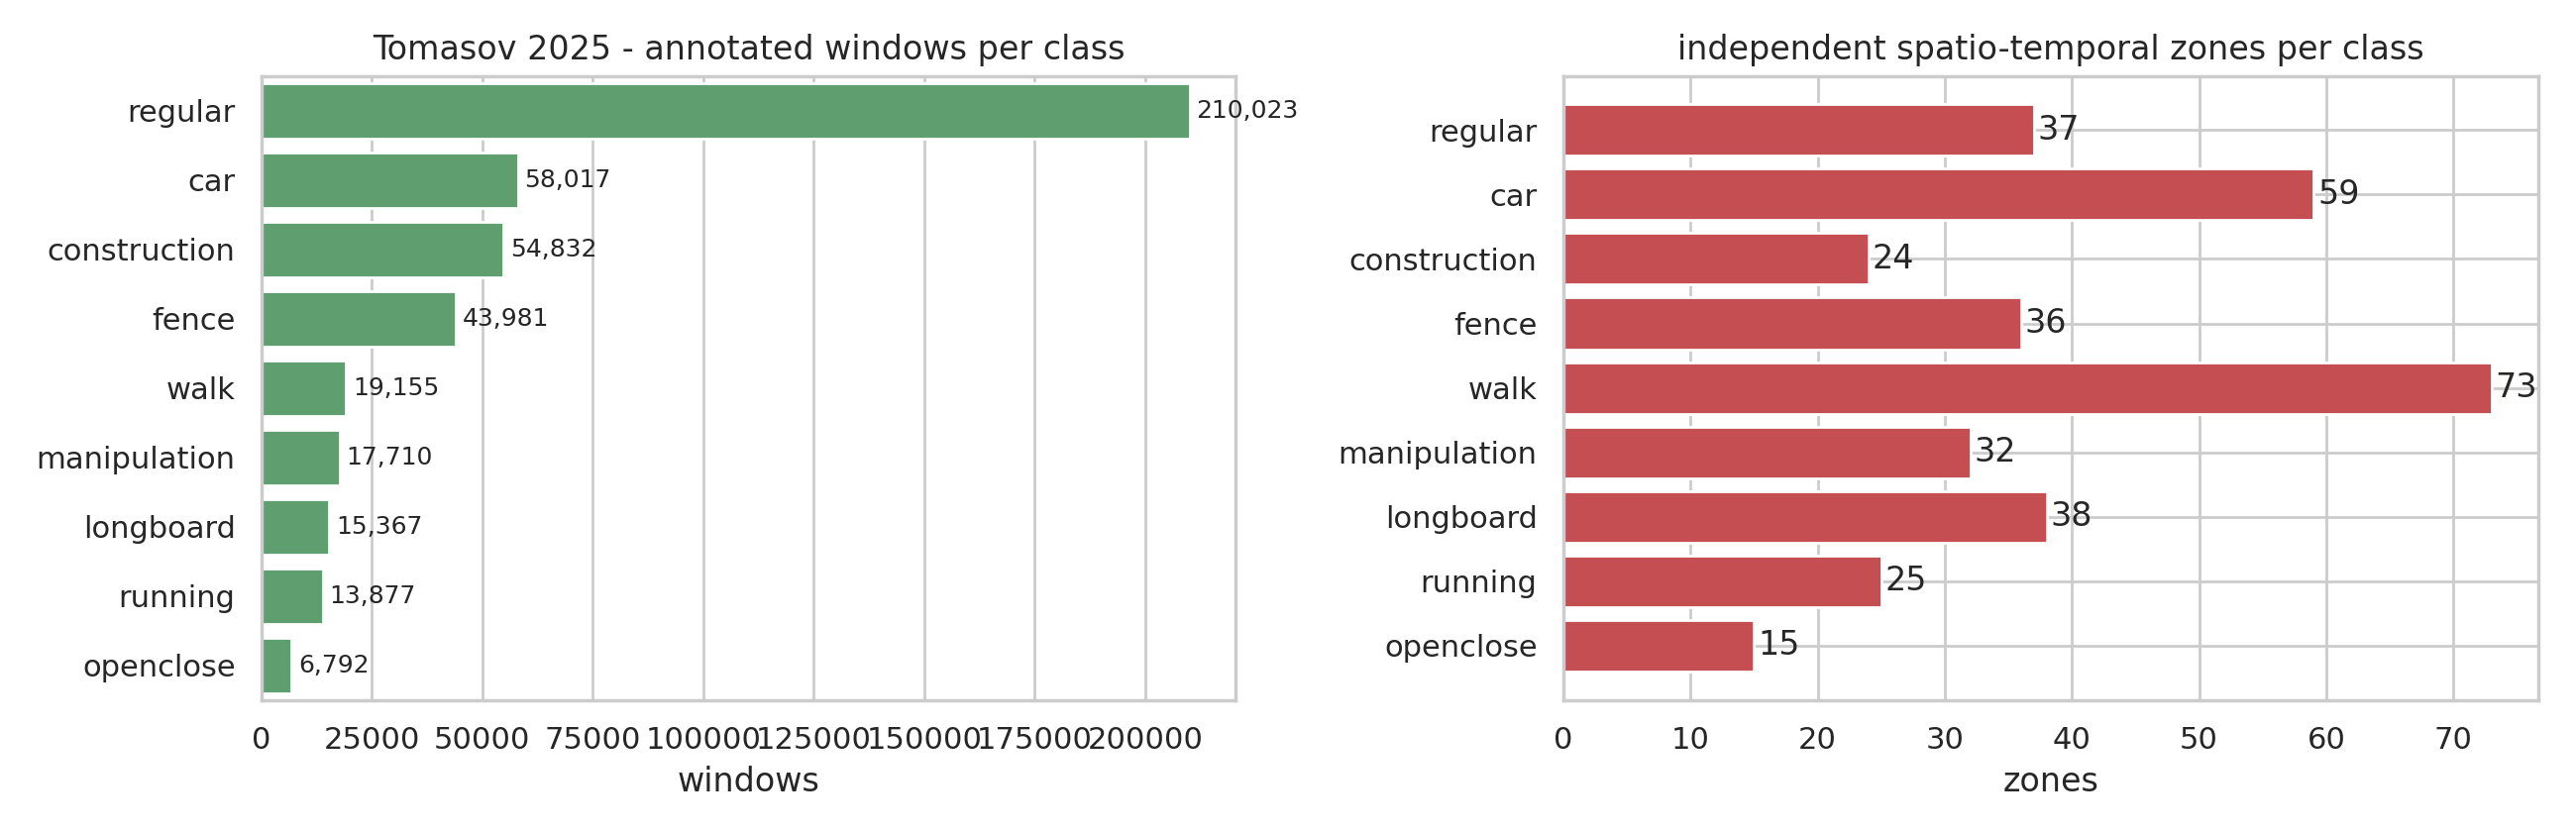
\includegraphics[width=0.95\textwidth,keepaspectratio]{Figures/fig27_tomasov_class_zone_counts.png}
\caption{Tomasov dataset inventory: annotated windows per class (left) and independent spatio-temporal zones per class (right). The zone count is the number of contiguous annotated regions and bounds how many independent groups any partition can draw on.}
\label{fig:tomasov_counts}
\end{figure}

Table~\ref{tab:dataset} records a fact that governs the whole analysis. Five of the nine Tomasov classes (\emph{construction}, \emph{manipulation}, \emph{openclose}, \emph{regular}, and \emph{running}) come from exactly one recording each, so for those classes recording identity and class identity are the same variable. No partition of this dataset can separate them; \refss{sec:chap3ConfoundDesign} describes the diagnostic designed to measure the consequence rather than assume it away.

\begin{figure}[!htbp]
\centering
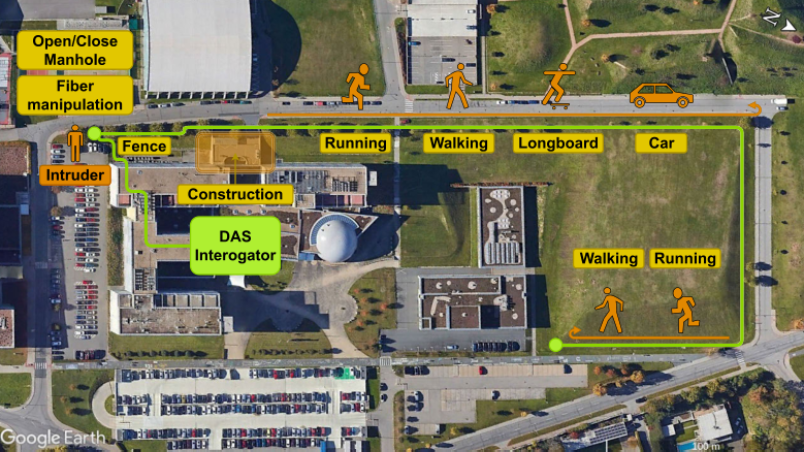
\includegraphics[width=0.85\textwidth]{Figures/fig04_campus_map.png}
\caption{Perimeter-security DAS setup and event labels along the monitored fibre path.}
\label{fig:campus_map}
\end{figure}

\subsubsection{Construction of Sample Manifests}
\label{sec:chap3Manifests}
\autoBookmark{subsubsec}{Construction of Sample Manifests}
Before any signal is read, each dataset is converted into a \emph{sample manifest}: a table with one row per analysis window that records the window's class label, its physical provenance, and the identifiers of every dependence group to which it belongs. The manifest is built from metadata alone (the annotation masks and the filenames), so it can be constructed, audited, and partitioned in seconds without loading the raw interrogator data. Every later stage, from feature extraction to final evaluation, is joined to the manifest through a unique sample identifier, which makes the manifest the single authoritative record of what each sample is and where it came from. Table~\ref{tab:manifest} lists the fields recorded for each dataset.

For Tomasov, labels are derived from the released annotation mask, a Boolean array over (time-block, locus) cells in which one block spans $H = 2{,}048$ raw samples. Each annotated cell whose block index $b$ leaves room for a complete window, $b \le n_{\mathrm{blocks}} - L/H$, becomes one manifest row, labelled with the event class of the recording in which it lies. The row stores the recording identifier, the block index, the locus, and the raw-sample interval $[bH,\, bH + L)$ that the window will read. Recording this interval explicitly is what later allows the leakage audit and the guard bands to be computed exactly rather than approximately. Acquisition parameters are read from the attributes of each HDF5 file rather than assumed, and all 16 recordings were confirmed to share a 20\,kHz pulse rate and $1{,}700$ loci. Because the annotations mark many loci within each block, the manifest is dense in space as well as in time: the \emph{regular} recording alone contributes $210{,}023$ windows drawn from 738 blocks and 622 loci.

For Cao, each \texttt{.mat} record becomes one manifest row, labelled by the class folder in which it is stored. The filename is parsed into acquisition date, operator, event token, session token, and record index, and the session identifier concatenates date, operator, class, and session token, because a session token is unique only within that combination. The acquisition date is kept separately as the grouping unit for the leave-one-date-out evaluation of \refss{sec:chap3ConfoundDesign}. The released folder, training or test, is also recorded, but only so that the released protocol can be audited; it plays no part in the partition used in this study. The zero-byte record noted in \refss{sec:chap3Dataset} is flagged at this stage and excluded, leaving $15{,}418$ rows.

\begin{table}[!htbp]
	\centering
	\caption{Contents of the sample manifests. The Tomasov split group is assigned during partitioning (\refss{sec:chap3Partitioning}); every other field is derived from the released metadata.}
	\label{tab:manifest}
	\small
	\setlength{\tabcolsep}{4pt}
	\begin{tabularx}{\textwidth}{@{}>{\raggedright\arraybackslash}p{2.7cm} >{\raggedright\arraybackslash}X >{\raggedright\arraybackslash}X@{}}
		\toprule
		\textbf{Field} & \textbf{Tomasov \etal\ 2025} & \textbf{Cao \etal\ 2023}\\
		\midrule
		Unit (one row)   & One annotated (time-block, locus) cell & One pre-segmented \texttt{.mat} record\\
		Label source     & Event class of the annotated recording & Class folder of the record\\
		Provenance       & Recording, block index, locus, raw-sample interval & Date, operator, session token, record index\\
		Split group      & Contiguous recording segment (154) & Recording session (441)\\
		Robustness group & Recording (16) & Acquisition date (10)\\
		Exclusions       & Blocks too close to the end of a stream to hold a full window & One zero-byte record\\
		Rows             & $439{,}754$ & $15{,}418$\\
		\bottomrule
	\end{tabularx}
\end{table}

\subsubsection{Identification of Leakage in the Released Protocols}
\label{sec:chap3LeakageAudit}
\autoBookmark{subsubsec}{Identification of Leakage in the Released Protocols}

\paragraph[Origin of the Investigation]{Origin of the Investigation.}
The leakage examined in this thesis was not anticipated at the outset. In the first design cycle, the pipeline was evaluated on the Tomasov dataset alone under a stratified random $80/10/10$ partition of analysis windows, the form of protocol used by the dataset's own authors and by several later studies (\refs{sec:chap2RelatedWorks}). Under that protocol the pipeline scored well across the whole taxonomy, including an $F_1$ of $0.72$ with $70\%$ recall on \emph{openclose}, the smallest class and one captured in a single recording. When the second design cycle added the Cao dataset to evaluate the design, the protocol had to be specified for data with a different structure, and this prompted a re-examination of the assumption on which the first cycle rested: that individual analysis windows are independent samples. The re-examination asked one question of each dataset, namely what the smallest unit of data is that can be treated as statistically independent of every other unit, and it answered that question from the way the data were generated rather than from model behaviour. It proceeded in five steps, and only the last required a model to be trained.

\paragraph[Step 1: Overlap Between Windows]{Step 1: Overlap Between Windows.}
The first step compared the window geometry with the annotation grid of the Tomasov release. A window of $L = 8{,}192$ samples spans $L/H = 4$ annotation blocks, so a window advanced by one block of $H = 2{,}048$ samples shares $L - H = 6{,}144$ samples, or $75\%$, with its predecessor; at the 256-sample stride adopted by the dataset's authors the shared fraction rises to $96.9\%$ (\reff{fig:window_overlap}). The overlap is spatial as well as temporal. Two windows annotated at the same block and at neighbouring loci read the same time interval, their 32-channel patches share 31 channels, and the loci themselves lie 1.02\,m apart and observe the same physical disturbance. A window-level random partition scatters these near-duplicates across training, validation, and test, so a test window can be matched to a training window that contains most of its raw samples, the same mechanism that inflates accuracy in sensor-based activity recognition~\cite{dehghani2019windows}.

\begin{figure}[!htbp]
\centering
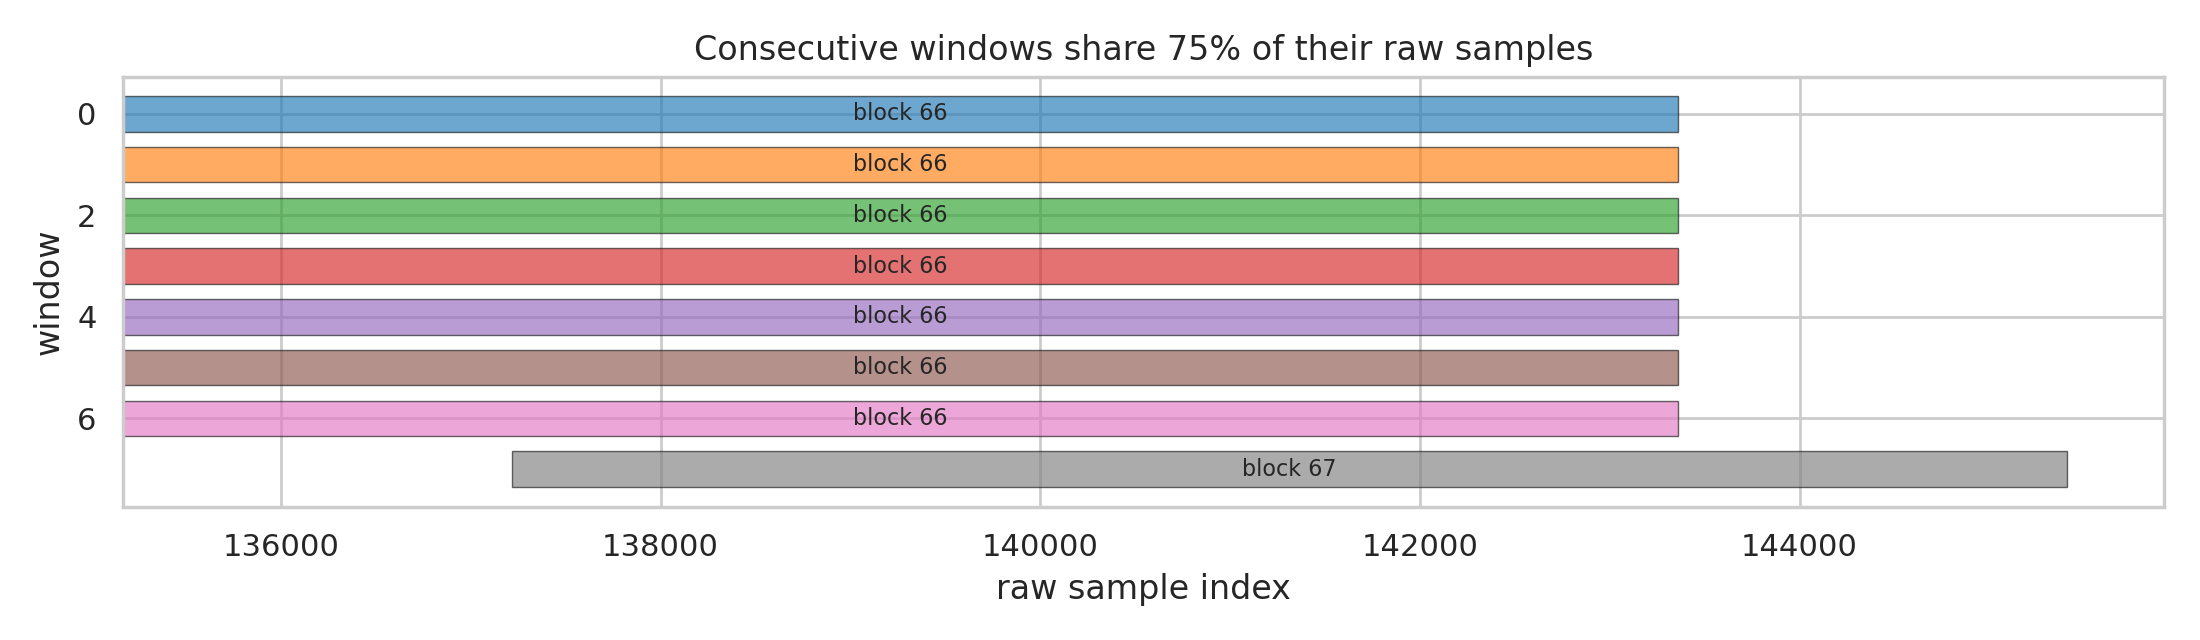
\includegraphics[width=0.9\textwidth,keepaspectratio]{Figures/fig14_window_overlap.png}
\caption{Consecutive analysis windows in the Tomasov dataset share $6{,}144$ of their $8{,}192$ raw samples. Under a random split these overlapping windows are distributed across training, validation, and test.}
\label{fig:window_overlap}
\end{figure}

\paragraph[Step 2: The Recording Inventory]{Step 2: The Recording Inventory.}
The second step tabulated the Tomasov windows by class and by recording (Table~\ref{tab:dataset}). The $439{,}754$ windows come from only 16 recordings, and five of the nine classes, \emph{openclose} among them, are each drawn from a single recording. For these classes the event label and the recording identity are the same variable, so any property of the recording, such as its noise floor, coupling, or local fibre geometry, predicts the label perfectly. This observation explained why the first-cycle result for \emph{openclose} deserved suspicion. All $6{,}792$ of its windows come from one recording spanning only 128 annotated blocks, about 13\,s of signal, so under a random partition almost every test window had near-duplicates from the same few seconds of the same recording in the training set.

\paragraph[Step 3: The Session Structure of the Cao Release]{Step 3: The Session Structure of the Cao Release.}
The Cao release seems at first to avoid the problem, because it ships as pre-segmented, non-overlapping records already divided into fixed training and test folders. Its filenames, however, follow the pattern \texttt{date\_operator\_event\_session\_data\_N}, which shows that many records were cut from each continuous recording session. Every record from one session shares the fibre state, coupling, background-noise realisation, and operator of that session, so the session rather than the record is the unit of independence, just as the subject rather than the record is the unit of independence in clinical sensor data~\cite{saeb2017usecase}. Whether the released partition respects that unit cannot be read from the folder structure; it had to be measured.

\paragraph[Step 4: Quantifying the Contamination]{Step 4: Quantifying the Contamination.}
Two audits turned these observations into measurements, and both operate on the manifests without reading any signal data. For Tomasov, which has no released partition, the audit applies the first-cycle protocol, a stratified random $80/10/10$ partition, to all $439{,}754$ annotated windows under the study's fixed seed. For every recording it marks each raw-sample block read by any training window and counts the test windows whose read interval intersects that training footprint. For Cao, the audit counts, for each of the 441 sessions recovered from the filenames, the records it contributes to each released folder, and flags a session as contaminated when both counts are non-zero. The Tomasov audit finds that all $43{,}976$ test windows (100\%) share raw samples with at least one training window. The Cao audit finds 423 of 441 sessions (95.9\%) contaminated, which places $3{,}083$ of the $3{,}084$ records in the released test folder in a session that also supplies training records. \refs{sec:resLeakage} reports both audits in full.

\paragraph[Step 5: Linking Contamination to Performance]{Step 5: Linking Contamination to Performance.}
Contamination shows that a protocol can be exploited, but not that reported accuracy was actually inflated. The final step tested that link directly through controlled comparisons in which a model is trained twice with every factor held fixed except the partition: once under the leakage-controlled partition developed below, and once under a random partition of the same windows. Any difference between the two arms is attributable to the protocol alone. These protocol-attribution experiments, defined in \refss{sec:chap3ConfoundDesign}, are applied to the reconstructed Tomasov CNN, to every feature configuration of the pipeline, and to five recent architectures. Chapter~\ref{chap:ResultsAndDiscussion} reports their results, together with the change in per-class performance once the leak is removed.

\paragraph[Leakage Pathways and Their Controls]{Leakage Pathways and Their Controls.}
The investigation established two leakage pathways that originate in the data. Three further pathways do not depend on the data at all: they arise in the modelling pipeline whenever a fitted component, whether a feature selector, a resampler, or a scaler, is exposed to rows that are later used for evaluation (\refss{sec:chap2LeakPipeline}). The controls applied to all five follow the recommendations summarised in Table~\ref{tab:leakage_controls}, and Table~\ref{tab:leak_pathways} lists each pathway with its control. The partitioning scheme of \refss{sec:chap3Partitioning} closes the two data pathways, and confining every fitted component to training rows (\refss{sec:chap3ModelReady}) closes the three pipeline pathways. Each control is enforced by the structure of the code or by an assertion that halts execution, not by convention.

\begin{table}[!htbp]
	\centering
	\caption{Leakage pathways addressed in this study and the control applied to each.}
	\label{tab:leak_pathways}
	\small
	\setlength{\tabcolsep}{4pt}
	\begin{tabularx}{\textwidth}{@{}>{\raggedright\arraybackslash}p{2.2cm} >{\raggedright\arraybackslash}X >{\raggedright\arraybackslash}X >{\raggedright\arraybackslash}p{1.9cm}@{}}
		\toprule
		\textbf{Pathway} & \textbf{Source} & \textbf{Control} & \textbf{Section}\\
		\midrule
		Sample level    & Overlapping Tomasov windows share raw samples in time and across adjacent loci & Blocked segments with guard bands; raw-sample disjointness asserted & \ref{sec:chap3Partitioning}\\
		Recording level & Windows from one session or recording share acquisition conditions & Whole-group assignment (Tomasov: recording segment; Cao: session); group disjointness asserted & \ref{sec:chap3Partitioning}\\
		Selection level & Feature selectors fitted on rows later used for evaluation & Selectors fitted on training rows only and refitted inside every cross-validation fold & \ref{sec:chap3FeatureSelection}\\
		Resampling level & Synthetic samples interpolated across partition boundaries & Resamplers fitted inside the training pipeline and bypassed at prediction & \ref{sec:chap3Balancing}\\
		Scaling level   & Scaling statistics computed on evaluation rows & Scaler fitted inside the training pipeline & \ref{sec:chap3ModelReady}\\
		\bottomrule
	\end{tabularx}
\end{table}

\subsubsection{Group-Aware Partitioning}
\label{sec:chap3Partitioning}
\autoBookmark{subsubsec}{Group-Aware Partitioning}
The partitioning scheme replaces both released protocols. It follows four rules, in the spirit of the blocked cross-validation that Roberts et al.\ recommend for data with temporal, spatial, or hierarchical structure~\cite{roberts2017crossvalidation}, of the subject-wise partitioning required when several samples come from one source~\cite{saeb2017usecase}, and of h-block and hv-block cross-validation, which remove a band of observations between training and test data~\cite{burman1994hblock,racine2000hvblock}. First, a partition boundary may fall only between whole groups of dependent samples, never inside one. Second, each dataset targets an approximate $80/10/10$ division into training, validation, and test sets. Third, every class must be present in every split, since per-class metrics are otherwise undefined. Fourth, the partition is computed once from the manifest, before any feature is extracted, and frozen to disk; every later experiment joins against the stored assignment and none re-derives it. Because the two datasets have different dependence structures, the first rule is implemented differently for each.

\paragraph[Tomasov: Blocked Partitioning by Equal-Mass Segments]{Tomasov: Blocked Partitioning by Equal-Mass Segments.}
Two simpler alternatives were ruled out first. Leave-one-recording-out partitioning cannot cover the full taxonomy, because each single-recording class would vanish from training whenever its recording is held out. Stratified group $k$-fold over fixed-duration zones balances the number of groups per fold rather than the number of windows, and a zone in this dataset holds anywhere from 30 to $8{,}000$ windows depending on how many loci the event touches; the resulting $92/5/2$ partition left \emph{openclose} with no test samples at all. The adopted scheme therefore partitions each recording internally along its timeline (Algorithm~\ref{alg:blocked}). The windows of a recording are ordered by block index and divided at the deciles of that ordering into ten contiguous segments of approximately equal \emph{window mass}, and each segment boundary is moved to a block boundary so that no block is shared between segments. A random offset $o_r \in \{0, \dots, 9\}$, drawn for each recording from a generator seeded with the study seed, selects segment $o_r$ for validation and segment $(o_r + 1) \bmod 10$ for test, and the remaining eight segments form the training set. Rotating the offset prevents the held-out data from always lying at the start or end of a recording, where acquisition drift would otherwise be confounded with the split. Each recording--segment pair is one split group, giving 154 groups in total.

\begin{algorithm}[!htbp]
	\caption{Blocked partitioning of one Tomasov recording with guard bands.}
	\label{alg:blocked}
	\DontPrintSemicolon
	\KwIn{Manifest rows of recording $r$ with block indices $b_i$; number of segments $S = 10$; window span $B = L/H = 4$ blocks; guard width $G = 4$ blocks; seeded generator $\rho$}
	\KwOut{Split tag and retention flag for every row of $r$}
	Sort the rows by $b_i$ and compute the rank quantile $q_i \in [0, 1)$ of each row\;
	$s_i \leftarrow \lfloor S\, q_i \rfloor$, then $s_i \leftarrow \min\{s_j : b_j = b_i\}$ so that no block spans two segments\;
	Draw an offset $o_r$ uniformly from $\{0, \dots, S - 1\}$ using $\rho$\;
	Tag segment $o_r$ as \textit{val}, segment $(o_r + 1) \bmod S$ as \textit{test}, and every other segment as \textit{train}\;
	\ForEach{split $k \in \{\textit{train}, \textit{val}, \textit{test}\}$}{
		$F_k \leftarrow \bigcup_{i \in k} \{b_i, \dots, b_i + B - 1\}$ \tcp*{footprint of $k$}
		$\hat{F}_k \leftarrow \{\, b : |b - b'| \le G \text{ for some } b' \in F_k \,\}$ \tcp*{dilate by $G$}
	}
	\ForEach{row $i$ assigned to split $k$}{
		$\mathrm{keep}_i \leftarrow \bigl[\, \{b_i, \dots, b_i + B - 1\} \cap \bigcup_{k' \neq k} \hat{F}_{k'} = \emptyset \,\bigr]$\;
	}
\end{algorithm}

\paragraph[Guard Bands]{Guard Bands.}
Assigning whole segments makes the split groups disjoint, but not the raw samples, because a training window that begins up to three blocks before a test segment reads blocks inside it. For each recording and split, the footprint of the split is therefore computed as the set of blocks read by any of its windows at any locus, and that footprint is dilated by a guard of $G = L/H = 4$ blocks, one full window length. Any window whose read interval intersects the dilated footprint of a different split is removed. Taking the footprint over all loci makes the guard conservative: after removal, windows in different splits share no time sample at any channel, which also eliminates the spatial near-duplicates identified in Step~1. Guard-band removal deletes $39{,}560$ windows, $9.00\%$ of the annotated set, and shifts the realised division from $79.98/9.96/10.06$ to $84.63/7.61/7.75$. The shift arises because every boundary costs each adjacent split a similar number of windows, which is a much larger fraction of a single validation or test segment than of the eight-segment training block. \reff{fig:split_timeline} shows the resulting assignment along each recording, with the guard bands visible as gaps.

\begin{figure}[!htbp]
\centering
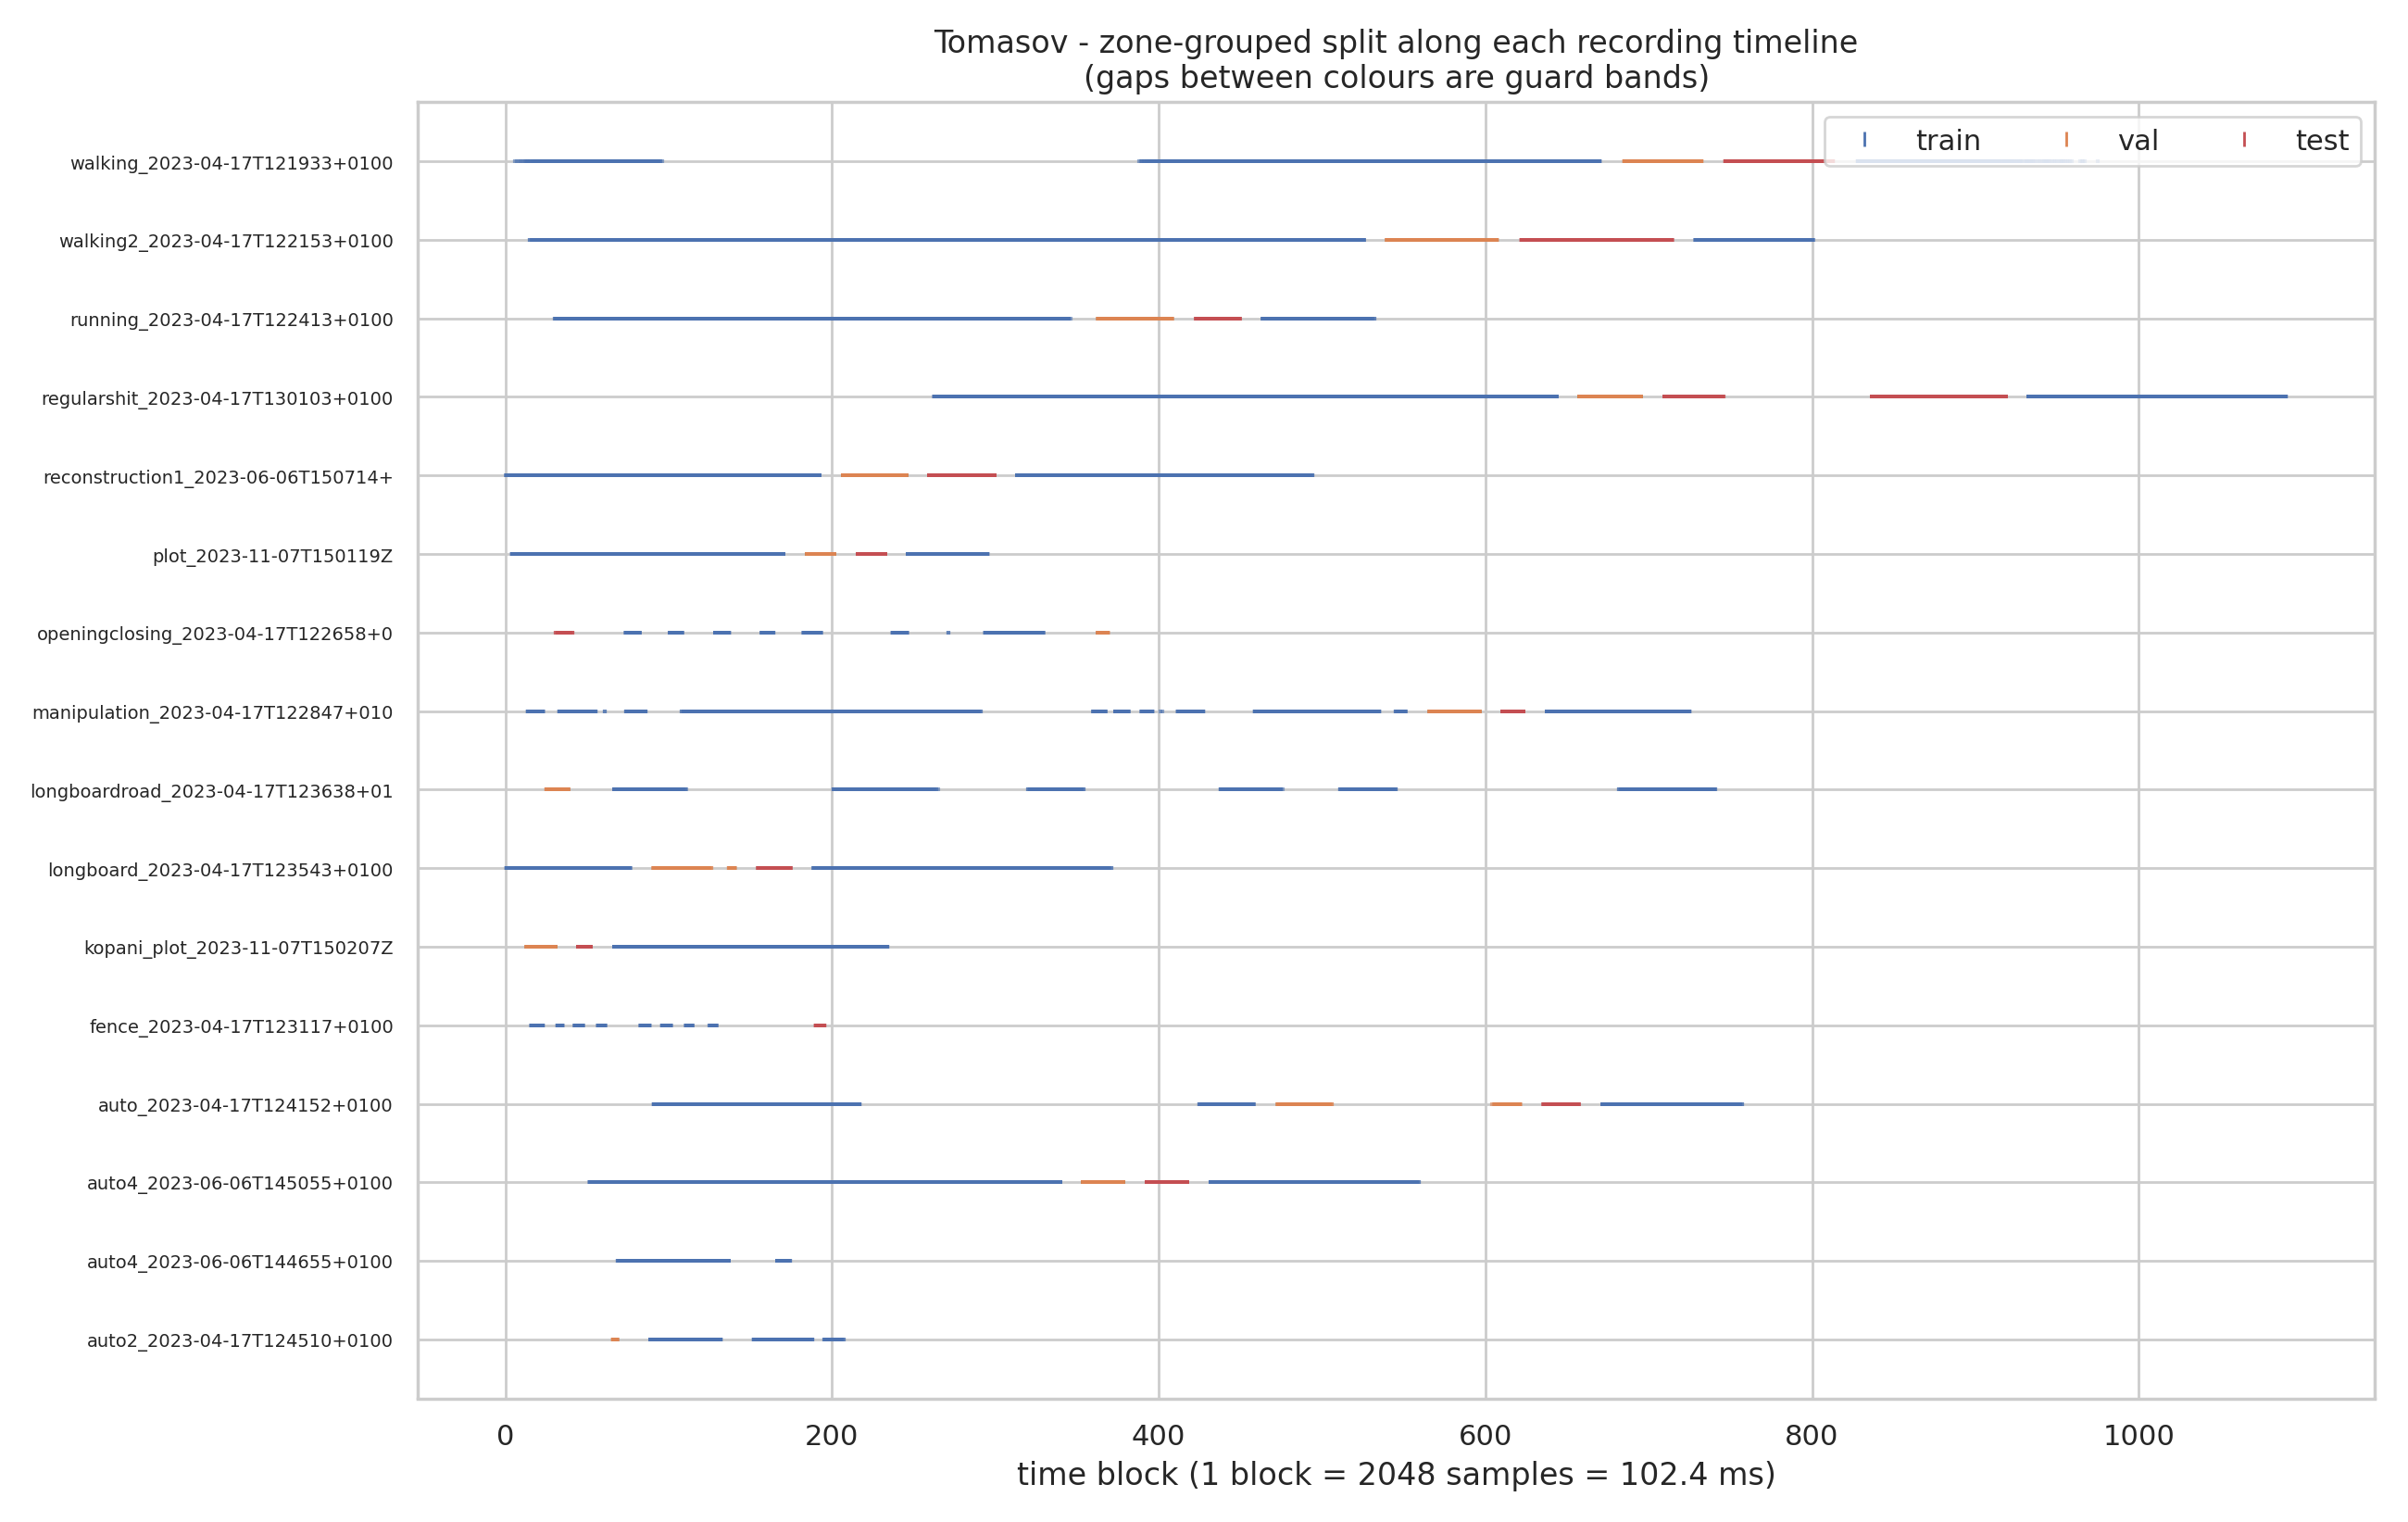
\includegraphics[width=0.95\textwidth,keepaspectratio]{Figures/fig15_split_timeline.png}
\caption{Blocked partitioning of the Tomasov dataset. Each row is one recording and colour denotes split; gaps are guard bands, removed so that no raw sample is shared between splits.}
\label{fig:split_timeline}
\end{figure}

\paragraph[Class Decimation After Partitioning]{Class Decimation After Partitioning.}
Three classes dominate the Tomasov annotations, and \emph{regular} alone accounts for $47.8\%$ of all windows. To stop these classes from dominating training, they are capped at $12{,}350$ (\emph{regular}), $29{,}010$ (\emph{car}), and $27{,}420$ (\emph{construction}) windows, the targets used in the first design cycle, retained for comparability. The first cycle decimated before partitioning; here decimation follows partitioning and guard-band removal, so that the split geometry cannot depend on which windows survive. Within every (class, split) cell the same fraction of windows is drawn at random under the fixed seed, which preserves each class's split proportions. Decimation removes a further $227{,}736$ windows and reduces the imbalance ratio from $30.9{:}1$ in the annotated set to $6.6{:}1$, leaving the $172{,}458$ windows on which features are extracted and every Tomasov result is computed. Because decimation only deletes whole windows, it can shrink but never enlarge the raw-sample footprint of any split, so it cannot reintroduce overlap. Cao is balanced to $1.3{:}1$ as released and is not decimated.

\paragraph[Cao: Session-Grouped Partitioning]{Cao: Session-Grouped Partitioning.}
For Cao the split group is the recording session. Sessions are distributed over ten folds by stratified group $k$-fold with shuffling under the fixed seed, which places each session in exactly one fold while keeping the class distribution of each fold as close to the overall distribution as indivisible sessions allow. Eight folds are merged into the training set, and the remaining two become the validation and test sets. Each record is a separate, non-overlapping segment, so no two records share raw samples and no guard band is needed. Sessions vary in size, so moving whole sessions cannot meet the target exactly; the realised division is $78.84/9.47/11.69$, with 351, 46, and 44 sessions in the three splits. The same operator or acquisition date may still appear in more than one split. This is deliberate, since forbidding it would leave several classes without training data, and the stricter question of generalisation to an unseen acquisition date is answered separately by the leave-one-date-out evaluation of \refss{sec:chap3ConfoundDesign}.

\paragraph[Verification]{Verification.}
Four properties are asserted in code before any model is trained, and the pipeline halts if any of them fails: (i) no split group appears in more than one split; (ii) no sample identifier is duplicated; (iii) for Tomasov, the sets of raw-sample blocks read by the three splits are pairwise disjoint within every recording; and (iv) every class is present in every split. The fourth property is checked rather than assumed. Aligning segments with blocks can merge neighbouring segments, and the guard bands can empty a short segment entirely, so an individual recording may contribute to fewer than three splits. In the final partition, two of the four \emph{car} recordings and one of the two \emph{longboard} recordings contribute no test windows, yet every class remains represented in every split. The full verification is run after guard-band removal and repeated on the decimated manifest, so the guarantees hold on the exact windows used for training and evaluation rather than on a superset of them. \refss{sec:chap3RealisedPartitions} reports the realised sizes at each stage.

\subsection{Signal Preprocessing}
\label{sec:chap3Preprocessing}
\autoBookmark{subsec}{Signal Preprocessing}
Preprocessing turns raw interrogator output into a quantity that a feature extractor can describe meaningfully. It matters more in DAS than in many sensing modalities, because the raw measurement carries several contaminants on different timescales, and any left in place would be absorbed into the descriptors as though it were information about the event. This subsection states what each operation removes, why the operations are ordered as they are, and what the chain costs. \reff{fig:example_window} shows one annotated Tomasov window before and after conditioning.

\begin{figure}[!htbp]
\centering
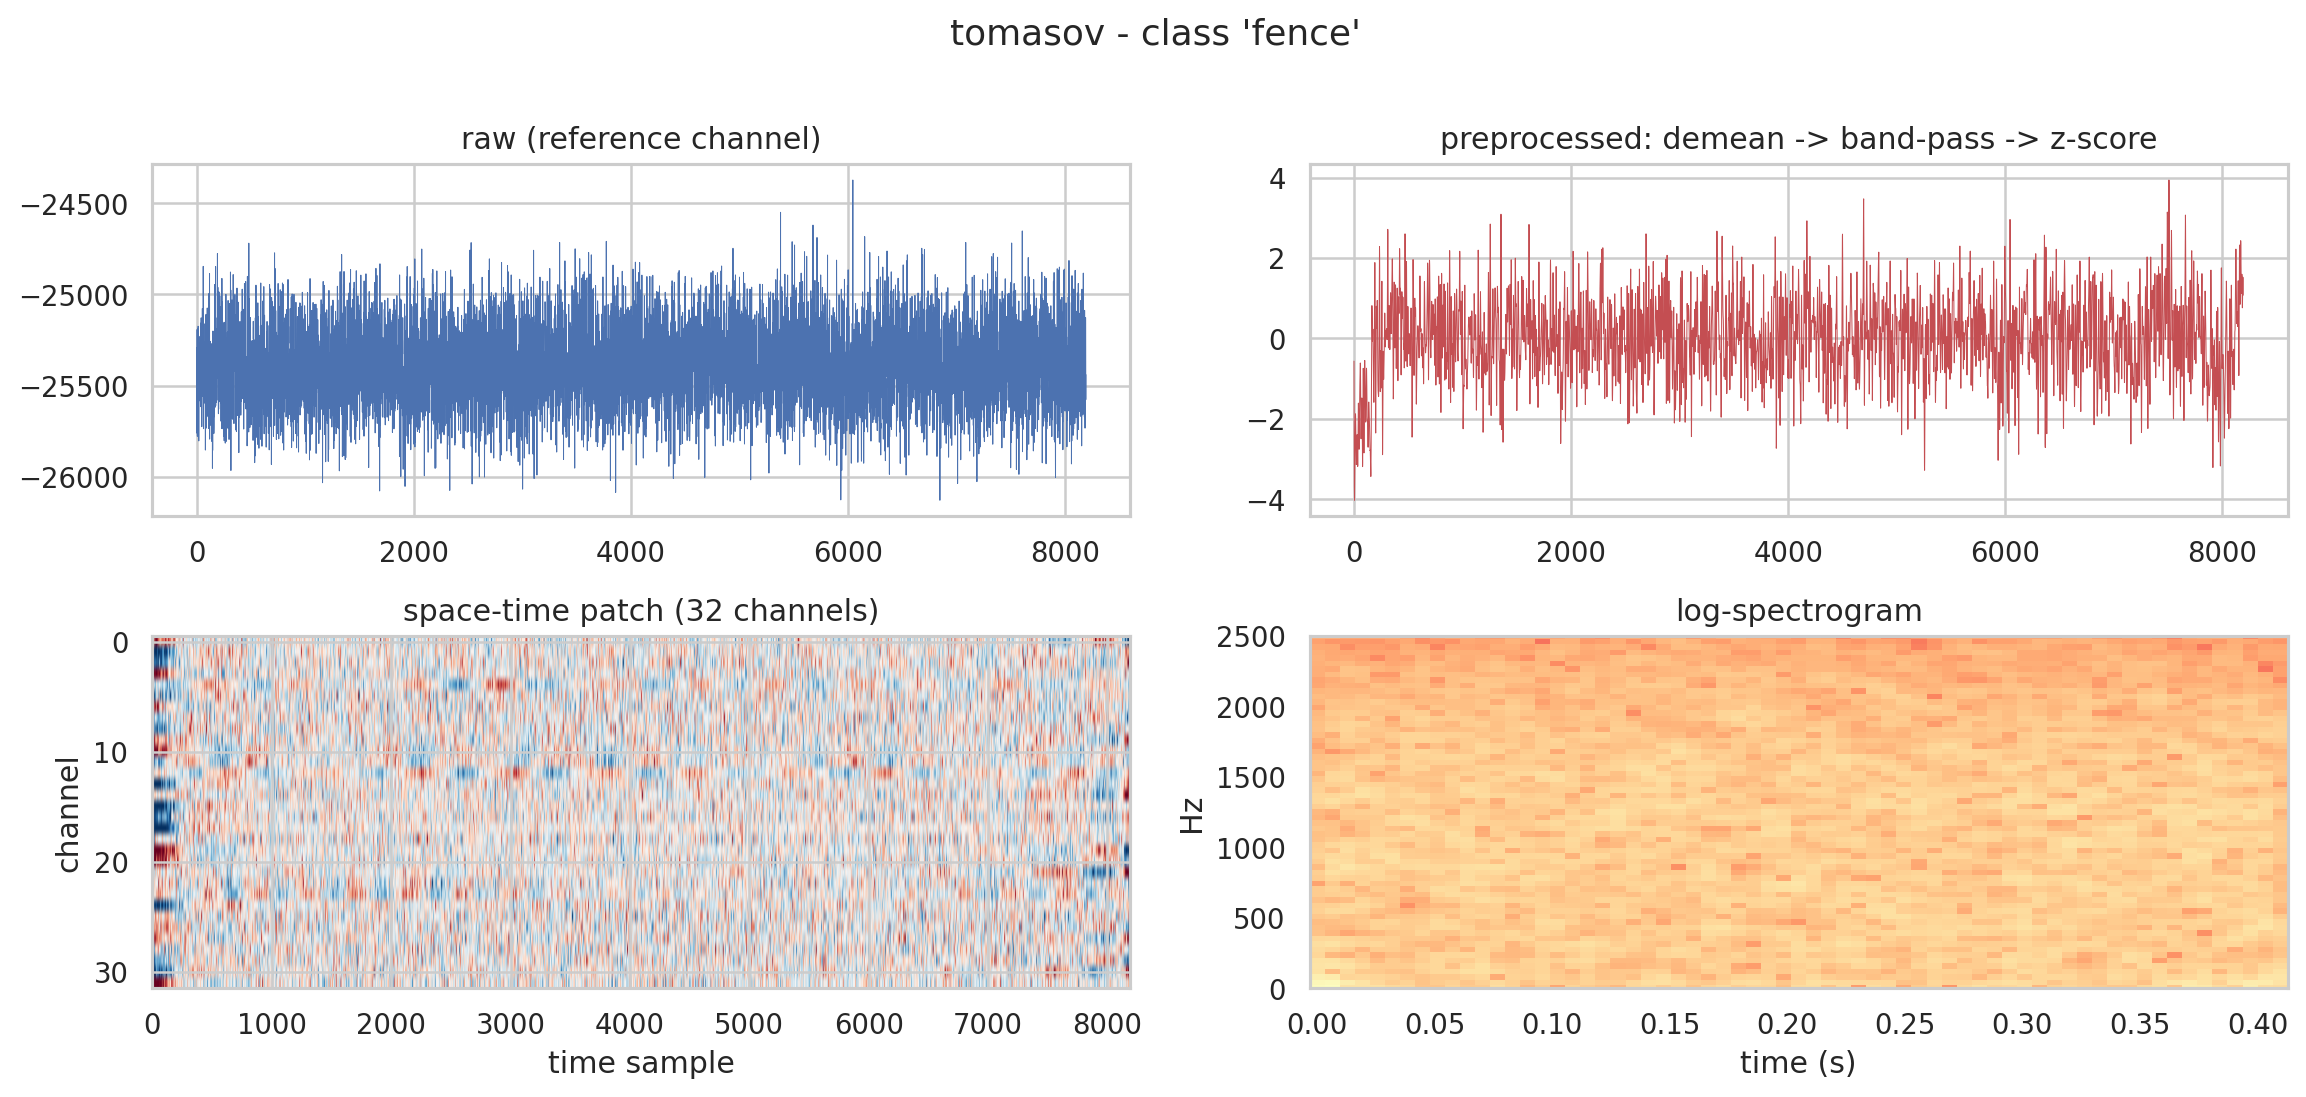
\includegraphics[width=0.95\textwidth,keepaspectratio]{Figures/fig28_example_window_fence.png}
\caption{One annotated \emph{fence} window from the Tomasov dataset: raw reference channel (top left), the same channel after demeaning, band-pass filtering, and z-scoring (top right), the 32-channel space--time patch used by the spatial extractor (bottom left), and the log-spectrogram used by the time--frequency extractor (bottom right).}
\label{fig:example_window}
\end{figure}

\subsubsection{The Raw Signal in DAS}
\label{sec:chap3RawSignal}
\autoBookmark{subsubsec}{The Raw Signal in DAS}
A single DAS channel records the optical phase, or the backscattered intensity, at one point along the fibre, and the recorded quantity superimposes four components on the vibration of interest. They operate on different timescales and call for different treatment, which is why the conditioning chain has three stages rather than one.

\begin{enumerate}[label=(\roman*), leftmargin=*, itemsep=3pt]
	\item \textbf{A large, slowly varying offset and drift.} Thermal expansion, laser wavelength drift, and slow strain accumulation produce a low-frequency component that often exceeds the event in magnitude. Left in place, it dominates every amplitude statistic and every low-frequency spectral bin.
	\item \textbf{Broadband instrument and shot noise.} Detector and digitisation noise extend across the full band, contributing energy unrelated to any event and varying with interrogator settings.
	\item \textbf{Coherent fading.} Backscatter from a given locus can interfere destructively, so that the channel intermittently loses sensitivity. This is a channel-specific, time-varying gain effect rather than additive noise, and it is one reason the spatial descriptors must be read with care.
	\item \textbf{Acquisition-specific gain.} The absolute amplitude scale depends on interrogator configuration, fibre coupling, and burial conditions, all fixed within a recording and different between recordings.
\end{enumerate}

Demeaning and band-pass filtering address components (i) and (ii), and amplitude normalisation addresses component (iv), for reasons given in \refss{sec:chap3Normalisation}. Component (iii) is a time-varying, channel-specific gain that cannot be estimated from a single window, so it is carried as a known limitation in the interpretation of the spatial domain rather than corrected. The subsections below define the unit of analysis and then take the three operations in the order in which they are applied.

\subsubsection{Windowing}
\label{sec:chap3Windowing}
\autoBookmark{subsubsec}{Windowing}
Both datasets are reduced to a common unit of analysis before conditioning. For Tomasov, the continuous stream is divided into windows of $T = 8{,}192$ samples advanced by $H = 2{,}048$ samples, matching the geometry on which the released annotation mask is defined: the mask marks (time-block, locus) cells where a block is $H$ raw samples, so a window beginning at block $b$ reads blocks $b$ to $b + L/H - 1$. This correspondence is what makes the guard-band computation of \refss{sec:chap3Partitioning} exact.

For Cao, records are already segmented at $10{,}000$ samples, and each record yields exactly one window. A centre crop of $8{,}192$ samples is taken, discarding 904 samples at each end, so that every window in the study has the same length and a single extractor serves both datasets. Because the authors clipped each record with the disturbance positioned mostly at its centre, the crop keeps the event and removes only the record margins. One window per record also means that Cao windows never overlap, which is why the sample-level pathway of Table~\ref{tab:leak_pathways} applies to Tomasov alone.

Two objects are produced per window and carried forward: a one-dimensional signal $x \in \mathbb{R}^{T}$, used by the time, frequency, and time--frequency extractors, and a two-dimensional space--time patch $X \in \mathbb{R}^{C \times T}$, used by the spatial extractor. For Tomasov, $C = 32$ loci centred on the annotated channel, and the one-dimensional signal is the centre channel of that patch. For Cao, $C = 12$ (all loci of the record), and the one-dimensional signal is the highest-energy channel, which corresponds to the disturbance location.

\subsubsection{Direct-Current Removal}
\label{sec:chap3DCRemoval}
\autoBookmark{subsubsec}{Direct-Current Removal}
The first operation subtracts the window mean:
\begin{equation}
	x^{(1)} = x - \mu_x, \qquad \mu_x = \frac{1}{T}\sum_{t=1}^{T} x_t .
	\label{eq:dcremoval}
\end{equation}
Demeaning precedes filtering for a practical reason. The band-pass filter is applied by forward--backward recursion, and a large constant offset at the boundaries of a finite window produces a transient that contaminates the first and last several hundred samples. Removing the offset first reduces that transient by roughly the size of the offset.

\subsubsection{Band-Pass Filtering}
\label{sec:chap3Filtering}
\autoBookmark{subsubsec}{Band-Pass Filtering}
A fourth-order Butterworth band-pass filter with cut-offs $f_{\mathrm{low}} = 20$\,Hz and $f_{\mathrm{high}} = 2000$\,Hz is applied next. The Butterworth response is chosen for its maximally flat passband, which avoids imposing ripple on the spectral shape that the frequency-domain descriptors are meant to measure. Fourth order gives a $-24$\,dB/octave roll-off, enough to suppress drift while keeping the transition band narrow enough not to attenuate the low end of the event band.

The band limits follow the physics of the events. The 20\,Hz lower edge sits above thermal and slow-strain drift and below the fundamental of footstep and vehicle excitation. The 2000\,Hz upper edge keeps the transient content of impacts and digging while discarding a region of the spectrum that, in these recordings, carries mainly instrument noise. The upper edge is clipped to $0.99$ times the Nyquist frequency of whichever dataset is being processed, so one specification serves both the 20\,kHz Tomasov stream and the slower Cao acquisition.

Filtering uses a second-order-sections implementation applied forward and backward. The cascaded biquad form stays numerically stable at these cut-off ratios, where a direct-form fourth-order filter would be poorly conditioned, and forward--backward application yields zero phase distortion. That matters because several descriptors (burst structure, envelope moments, spatial-centroid trajectory) depend on the temporal position of signal features. The cost is a doubling of the effective filter order, which is accounted for in the stated roll-off. Writing $\mathcal{H}_{\mathrm{BP}}(\cdot)$ for this operation,
\begin{equation}
	x^{(2)} = \mathcal{H}_{\mathrm{BP}}\!\left(x^{(1)}\right).
	\label{eq:bandpass}
\end{equation}

\subsubsection{Amplitude Normalisation}
\label{sec:chap3Normalisation}
\autoBookmark{subsubsec}{Amplitude Normalisation}
The final operation standardises the filtered window to zero mean and unit variance:
\begin{equation}
	\tilde{x} = \frac{x^{(2)} - \mu_{\mathcal{H}}}{\sigma_{\mathcal{H}}},
	\label{eq:zscore}
\end{equation}
where $\mu_{\mathcal{H}}$ and $\sigma_{\mathcal{H}}$ are the mean and standard deviation of the filtered signal. The implementation evaluated in this thesis adds $\epsilon = 10^{-12}$ to the denominator as a guard against silent channels, a choice whose side effect is examined in \refss{sec:chap5LimResidue}. Combining Equations~\eqref{eq:dcremoval}--\eqref{eq:zscore} gives the complete chain:
\begin{equation}
	\tilde{x} = \frac{\mathcal{H}_{\mathrm{BP}}(x - \mu_x) - \mu_{\mathcal{H}}}{\sigma_{\mathcal{H}}}.
	\label{eq:preprocess}
\end{equation}

This step needs justification, because discarding absolute amplitude discards real information: a passing vehicle does excite the fibre more strongly than a footstep. The decision rests on the group structure of \refss{sec:chap3Dataset}. Absolute amplitude in DAS is set by interrogator gain and fibre coupling, constant within a recording and different between recordings. With five of nine Tomasov classes drawn from a single recording each, an amplitude-preserving representation would hand the classifier a near-perfect recording fingerprint, and with it a shortcut to the label that no deployment could reproduce. Per-window normalisation is designed to remove that shortcut. It is therefore a leakage control first and a numerical convenience second, and its measured cost is accepted.

Two consequences follow. A few amplitude descriptors become constant by construction, since after normalisation the window mean is zero and the standard deviation one; the variance filter in the selection ensemble (\refss{sec:chap3Phase3}) removes them, which is one of the roles that filter serves. A ratio descriptor defined as the coefficient of variation would divide by a mean that is now zero, so its slot in the time-domain vector is taken by the scale-invariant ratio of root-mean-square to median absolute deviation, which measures the same notion of peakedness without the singularity.

\subsubsection{Properties of the Chain}
\label{sec:chap3PreprocProperties}
\autoBookmark{subsubsec}{Properties of the Chain}
Three properties of the chain matter for the validity of the evaluation. It is \textbf{stateless}: every parameter used to transform a window is computed from that window alone, so preprocessing cannot transfer information between samples or splits and may safely be applied before partitioning, whereas classifier feature scaling may not and is placed inside the training pipeline. It is \textbf{identical across datasets}: the same three operations with the same parameters, apart from Nyquist clipping, are applied to both acquisitions, so any difference in outcome is attributable to the data. And it is \textbf{applied per channel} for the two-dimensional patch: Equations~\eqref{eq:dcremoval}--\eqref{eq:zscore} are applied independently to each of the $C$ channels, which removes the per-channel gain differences caused by coupling variation and fading. It also gives every channel the same total energy, a consequence taken up in \refss{sec:chap3SpatialFeatures}.

\subsubsection{Computational Cost}
\label{sec:chap3PreprocCost}
\autoBookmark{subsubsec}{Computational Cost}
Preprocessing is cheap relative to feature extraction. The dominant term is the forward--backward filter, $\mathcal{O}(T)$ per channel with a small constant, applied $C$ times for the patch. On the target embedded platform conditioning takes a negligible fraction of the per-window budget reported in \refss{sec:chap3Efficiency}, which the time--frequency descriptors dominate by two orders of magnitude. The preprocessing parameters were therefore chosen on signal-quality grounds without a runtime constraint.

\subsection{Multi-Domain Feature Extraction and Fusion}
\label{sec:chap3Phase2}
\autoBookmark{subsec}{Multi-Domain Feature Extraction and Fusion}
Feature extraction builds a compact, discriminative description of each preprocessed window. Instead of relying on one representation, handcrafted descriptors are drawn from four complementary domains (\reff{fig:feature_extraction}). Time-domain descriptors capture amplitude and morphology, frequency-domain descriptors capture spectral structure, time--frequency descriptors capture non-stationary behaviour, and spatial and spatio-temporal descriptors exploit how energy localises and propagates across channels. Each family is defined below, and Table~\ref{tab:dimensionality} collects the counts.

\WarningFilter[frameworkfloat]{latex}{Float too large for page}
\ActivateWarningFilters[frameworkfloat]
\clearpage
\begin{landscape}
\makeatletter
\def\LS@rot{%
    \setbox\@outputbox\vbox{\hbox{\rotatebox[origin=c]{-90}{\box\@outputbox}}}%
}
\PLS@Rotate{270}
\makeatother
\begin{figure}[p]
    \centering
    \vspace*{-2.5cm}
    \makebox[\linewidth][c]{%
        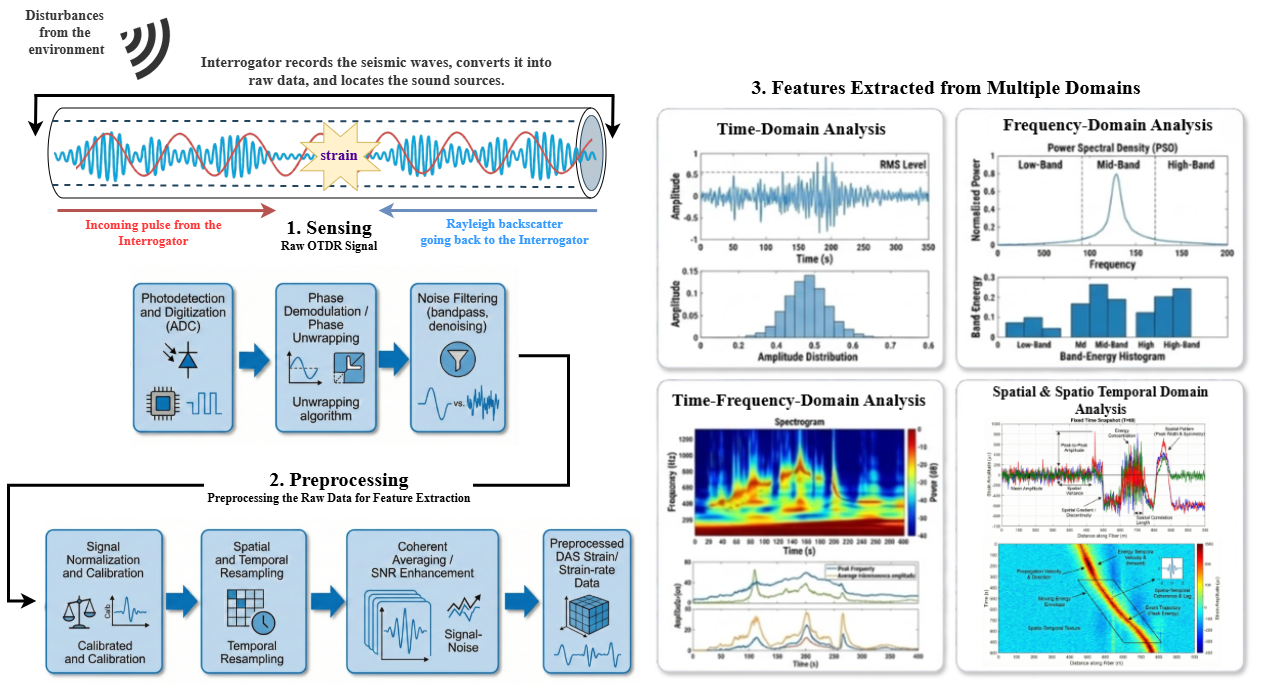
\includegraphics[
            width=0.88\paperheight,
            height=0.84\paperwidth,
            keepaspectratio
        ]{Figures/fig05_FE_pipeline.png}%
    }
    \caption{Feature extraction pipeline for DAS, spanning the time, frequency, time--frequency, and spatial/spatio-temporal domains.}
    \label{fig:feature_extraction}
\end{figure}
\end{landscape}
\DeactivateWarningFilters[frameworkfloat]
\clearpage

\subsubsection{Time-Domain Features}
\label{sec:chap3TimeFeatures}
\autoBookmark{subsubsec}{Time-Domain Features}
Time-domain features summarise amplitude, variability, and temporal morphology, and their low cost makes them attractive for real-time pipelines. A total of 112 are computed per window in eight groups: basic statistics, energy and power, temporal activity, slope and derivative measures, nonlinear descriptors, envelope metrics, burst structure, and histogram descriptors (Table~\ref{tab:timefeatures}). Let $x = [x_1, \ldots, x_N]$ denote a preprocessed window.

The standard moments, mean ($\mu$), variance ($\sigma^2$), skewness ($\gamma_1$), and kurtosis ($\gamma_2$), are
\begin{equation}
	\mu = \frac{1}{N}\sum_{i=1}^{N} x_i, \qquad \sigma^2 = \frac{1}{N}\sum_{i=1}^{N}(x_i - \mu)^2,
	\label{eq:meanvar}
\end{equation}
\begin{equation}
	\gamma_1 = \frac{\frac{1}{N}\sum_{i=1}^{N}(x_i - \mu)^3}{(\sigma^2)^{3/2}}, \qquad
	\gamma_2 = \frac{\frac{1}{N}\sum_{i=1}^{N}(x_i - \mu)^4}{(\sigma^2)^2}.
	\label{eq:skewkurt}
\end{equation}
Further statistics include percentiles, the interquartile range, the median absolute deviation, and the zero fraction. Energy features quantify signal strength through the root-mean-square value and the signal energy,
\begin{equation}
	\mathrm{RMS} = \sqrt{\frac{1}{N}\sum_{i=1}^{N} x_i^2}, \qquad E_{\mathrm{signal}} = \sum_{i=1}^{N} x_i^2,
	\label{eq:rmsenergy}
\end{equation}
and shape factors such as the crest factor detect transient peaks:
\begin{equation}
	\mathrm{CF} = \frac{\max(|x|)}{\mathrm{RMS}}.
	\label{eq:crest}
\end{equation}
The window is also divided into $K = 10$ segments to compute segment energies together with their entropy, centroid, spread, and Gini coefficient. Temporal activity is described by the zero-crossing rate, peak and valley counts, activity factors, and autocorrelation statistics, where
\begin{equation}
	\mathrm{ZCR} = \frac{1}{2(N-1)}\sum_{i=1}^{N-1} \bigl|\operatorname{sgn}(x_{i+1}) - \operatorname{sgn}(x_i)\bigr| \times f_s .
	\label{eq:zcr}
\end{equation}
Slope features include the mean and variance of the first difference ($\Delta x_i = x_{i+1} - x_i$) and of the second difference, together with slope-sign changes and waveform length. The Hjorth parameters, activity ($A$), mobility ($M$), and complexity ($C$), capture signal dynamics:
\begin{equation}
	A = \operatorname{var}(x), \qquad
	M = \sqrt{\frac{\operatorname{var}(\Delta x)}{\operatorname{var}(x)}}, \qquad
	C = \frac{\sqrt{\operatorname{var}(\Delta^2 x)/\operatorname{var}(\Delta x)}}{M}.
	\label{eq:hjorth}
\end{equation}
The Katz fractal dimension, from the curve length $L$ and maximum displacement $d$, is
\begin{equation}
	D_K = \frac{\log_{10}(N)}{\log_{10}(N) + \log_{10}(d/L)},
	\label{eq:katz}
\end{equation}
and the Higuchi fractal dimension and Teager--Kaiser energy complete the nonlinear group. Hilbert-envelope statistics describe modulation, and thresholding the envelope yields burst count, rate, duration, gap, and occupancy.

\begin{table}[!htb]
	\centering
	\caption{Summary of time-domain feature groups.}
	\label{tab:timefeatures}
	\small
	\setlength{\tabcolsep}{4pt}
	\renewcommand{\arraystretch}{0.95}
	\begin{tabularx}{\textwidth}{@{}>{\raggedright\arraybackslash}p{3.1cm} c >{\raggedright\arraybackslash}X@{}}
		\toprule
		\textbf{Feature Group} & \textbf{Count} & \textbf{Description}\\
		\midrule
		Basic statistical   & 26       & Central tendency, dispersion, percentiles, distribution shape, zero fraction.\\
		Energy \& power     & $13 + K$ & RMS, energy, shape factors, and $K = 10$ segment energies with their entropy, centroid, spread, and Gini coefficient.\\
		Temporal patterns   & 19       & Zero crossings, peak and valley statistics, activity factors, autocorrelation.\\
		Slope \& derivative & 7        & First and second differences, slope-sign changes, waveform length.\\
		Nonlinear descriptors & 7      & Hjorth parameters, Katz and Higuchi fractal dimensions, Teager--Kaiser energy.\\
		Envelope-based      & 6        & Moments, entropy, and crest of the Hilbert envelope.\\
		Burst structure     & 6        & Burst count, rate, duration, gap, and occupancy.\\
		Histogram-based     & 18       & 16-bin amplitude histogram with entropy and contrast.\\
		\midrule
		\textbf{Total}      & \textbf{112} & \\
		\bottomrule
	\end{tabularx}
\end{table}

\subsubsection{Frequency-Domain Features}
\label{sec:chap3FreqFeatures}
\autoBookmark{subsubsec}{Frequency-Domain Features}
Frequency-domain features summarise how vibration energy is distributed across frequencies and separate events with distinct spectral signatures. Each window is transformed with the real-valued FFT and 90 descriptors are extracted (Table~\ref{tab:freqfeatures}). The spectrum of a window $x[n]$ is
\begin{equation}
	X[k] = \sum_{n=0}^{N-1} x[n]\, e^{-j 2\pi k n / N}, \qquad k = 0, 1, \ldots, \tfrac{N}{2},
	\label{eq:fft}
\end{equation}
from which the magnitude spectrum $M[k] = |X[k]|$ and the power spectrum $P[k] = |X[k]|^2$ follow. The spectral centroid $C$ and spread $S$ are
\begin{equation}
	C = \frac{\sum_{k=0}^{K} f_k \, M[k]}{\sum_{k=0}^{K} M[k]}, \qquad
	S = \sqrt{\frac{\sum_{k=0}^{K} (f_k - C)^2 \, M[k]}{\sum_{k=0}^{K} M[k]}},
	\label{eq:centroid}
\end{equation}
where $f_k$ is the frequency at bin $k$. The Shannon spectral entropy of the normalised power spectrum $p_k = P[k] / \sum P[k]$ is
\begin{equation}
	H = -\sum_{k=0}^{K} p_k \log_2 (p_k + \epsilon),
	\label{eq:entropy}
\end{equation}
with $\epsilon$ a small constant that prevents a logarithmic singularity. Band powers are computed in absolute and relative form over seven bands: $[0,50]$, $[50,100]$, $[100,200]$, $[200,400]$, $[400,800]$, $[800,1600]$, and $[1600, f_s/2]$\,Hz.

\begin{table}[!htbp]
	\centering
	\caption{Summary of frequency-domain feature groups.}
	\label{tab:freqfeatures}
	\small
	\begin{tabularx}{\textwidth}{@{}>{\raggedright\arraybackslash}p{3.4cm} c >{\raggedright\arraybackslash}X@{}}
		\toprule
		\textbf{Feature Group} & \textbf{Count} & \textbf{Description}\\
		\midrule
		Basic spectral statistics & 8  & Mean, std, min, max, and range of magnitude and power.\\
		Spectral shape            & 8  & Centroid, spread, roll-off, flatness, skewness, kurtosis, slope.\\
		Peak-related              & 6  & Dominant and secondary peak frequency and amplitude; peak count and ratio.\\
		Band powers               & 14 & Absolute and relative power in seven bands.\\
		DAS band ratios           & 7  & Low/mid/high energy ratios, fractions, and high-tail ratio.\\
		Spectral entropy          & 3  & Shannon entropy, R\'enyi entropy, spectral decrease.\\
		PSD statistics            & 3  & Max, min, and range of power spectral density.\\
		Histogram features        & 33 & 32-bin magnitude histogram and its entropy.\\
		Cepstral coefficients     & 8  & First eight real cepstral coefficients.\\
		\midrule
		\textbf{Total}            & \textbf{90} & \\
		\bottomrule
	\end{tabularx}
\end{table}

\subsubsection{Time--Frequency-Domain Features}
\label{sec:chap3TFFeatures}
\autoBookmark{subsubsec}{Time--Frequency-Domain Features}
DAS event signatures are often non-stationary, so time--frequency representations are used to model temporal evolution and spectral content jointly. A hybrid set of 739 features combines STFT statistics, wavelet decompositions, texture and geometry descriptors of a quantised log-spectrogram, and DAS-specific indices (Table~\ref{tab:tffeatures}). The magnitude spectrogram $S(m,k)$ is computed with a Hann window, $N_{\mathrm{FFT}} = 512$, and a hop of 128 samples,
\begin{equation}
	S(m,k) = \left| \sum_{n=0}^{N_{\mathrm{FFT}}-1} x[n]\, w[n - mH]\, e^{-j 2\pi k n / N_{\mathrm{FFT}}} \right|,
	\label{eq:stft}
\end{equation}
which gives a $257 \times 61$ spectrogram per window. A coarser $4096/2048$ setting was rejected because it yields only about five frames, too few for the texture descriptors that follow. From $S(m,k)$ are derived global power statistics, temporal-envelope and spectral-marginal descriptors, inter-frame dynamics (flux, divergence, coherence, novelty), a modulation spectrum over 12 critical bands, and the energy in five DAS-relevant bands. Multi-resolution transient behaviour is captured by the discrete wavelet transform (up to level 6) and the wavelet packet transform (full decomposition to level 4, 16 sub-bands), both with the Daubechies-4 wavelet. For each coefficient set $c_i$, statistical moments and the Teager--Kaiser energy
\begin{equation}
	\Psi\bigl[c_i[n]\bigr] = c_i[n]^2 - c_i[n-1]\cdot c_i[n+1]
	\label{eq:tkeo}
\end{equation}
are computed. The log-spectrogram is then quantised to 32 levels, and grey-level co-occurrence statistics, local binary patterns, histogram-of-oriented-gradient features, and morphological descriptors of the binarised time--frequency mask are extracted. Four DAS-specific indices (tonal, transient, cyclostationary, and low--high band ratio) complete the set.

\begin{table}[!htbp]
	\centering
	\caption{Summary of time--frequency feature groups.}
	\label{tab:tffeatures}
	\small
	\begin{tabularx}{\textwidth}{@{}>{\raggedright\arraybackslash}p{3.6cm} >{\raggedright\arraybackslash}X c@{}}
		\toprule
		\textbf{Feature Group} & \textbf{Description} & \textbf{Count}\\
		\midrule
		STFT global power      & Distributional descriptors of spectrogram power (statistics, quantiles, shape moments, entropy). & 16\\
		Temporal envelope ($E_t$) & Statistics of the frequency-integrated power envelope. & 13\\
		Spectral marginal ($E_f$) & Descriptors of the time-integrated spectral distribution. & 21\\
		Spectral dynamics      & Inter-frame flux, divergence, coherence, and novelty. & 8\\
		Modulation spectrum    & Modulation centroid, spread, and entropy across 12 critical bands. & 36\\
		Band power             & Energy in five DAS-relevant bands (0--20, 20--50, 50--150, 150--300, 300--500\,Hz). & 5\\
		DWT features           & Daubechies-4 DWT (levels 0--6): coefficient statistics and TKEO summaries. & 140\\
		WPT features           & Wavelet packet descriptors (level 4, 16 sub-bands): statistics, energy, entropy, ratios. & 357\\
		GLCM texture           & Grey-level co-occurrence statistics over multiple distances and orientations. & 80\\
		LBP histogram          & 32-bin local binary pattern histogram of the quantised spectrogram. & 32\\
		HOG-like features      & 16-bin histogram of oriented gradients of time--frequency edges. & 16\\
		TF geometry            & Morphological descriptors of the binarised time--frequency mask. & 8\\
		TF distribution        & Occupancy and anisotropy measures. & 3\\
		DAS-specific metrics   & Tonal, transient, and cyclostationary indices; low--high band ratio. & 4\\
		\midrule
		\textbf{Total}         & & \textbf{739}\\
		\bottomrule
	\end{tabularx}
\end{table}

\subsubsection{Spatial and Spatio-Temporal Features}
\label{sec:chap3SpatialFeatures}
\autoBookmark{subsubsec}{Spatial and Spatio-Temporal Features}
Unlike a single-channel acoustic sensor, DAS records synchronised measurements across many channels. Each window is modelled as a patch $X \in \mathbb{R}^{C \times T}$, and 61 descriptors quantify how energy localises, spreads, and fragments across channels (Table~\ref{tab:spatialfeatures}). Let $E_c$ denote the energy of channel $c$,
\begin{equation}
	E_c = \sum_{t=1}^{T} |X_{c,t}|^2, \qquad c = 1, \ldots, C,
	\label{eq:channelenergy}
\end{equation}
with total energy $E_{\mathrm{tot}} = \sum_{c} E_c$ and normalised weights $w_c = E_c / (E_{\mathrm{tot}} + \epsilon)$, $\epsilon = 10^{-12}$. The spatial centroid and spread are
\begin{equation}
	\mu_{sp} = \sum_{c=1}^{C} c\, w_c, \qquad
	\sigma_{sp} = \sqrt{\sum_{c=1}^{C} (c - \mu_{sp})^2\, w_c},
	\label{eq:spatialcentroid}
\end{equation}
and the inequality of the channel-energy distribution is the Gini coefficient of the sorted energies $E_{(k)}$:
\begin{equation}
	\mathrm{Gini}(E) = \frac{C + 1 - 2\left(\dfrac{\sum_{k=1}^{C}(C + 1 - k)\, E_{(k)}}{\sum_{k=1}^{C} E_k}\right)}{C}.
	\label{eq:gini}
\end{equation}
Further descriptors capture spatial gradient and roughness (inter-channel differences, edge density, smoothness) and the clustering of active channels. The spatio-temporal group tracks the spatial-centroid trajectory across coarse temporal bins and reports its velocity, directionality, linearity, and variance, together with global patch statistics, the temporal activity profile, gradient and texture measures, and coarse histogram statistics.

\begin{table}[!htb]
	\centering
	\caption{Summary of spatial and spatio-temporal feature groups.}
	\label{tab:spatialfeatures}
	\small
	\setlength{\tabcolsep}{4pt}
	\renewcommand{\arraystretch}{0.95}
	\begin{tabularx}{\textwidth}{@{}>{\raggedright\arraybackslash}p{3.1cm} >{\raggedright\arraybackslash}X c@{}}
		\toprule
		\textbf{Feature Group} & \textbf{Description} & \textbf{Count}\\
		\midrule
		\multicolumn{3}{@{}l}{\textit{Spatial-domain features (from the channel-energy distribution)}}\\[2pt]
		Localisation \& extent     & Centroid, spread, width, argmax, and active-channel counts at thresholds. & 7\\
		Distribution \& shape      & Quantiles, skewness, kurtosis, Gini, entropy, flatness, top-channel fractions. & 10\\
		Gradient \& roughness      & Inter-channel gradient statistics, edge density, smoothness, total variation. & 7\\
		Clustering                 & Cluster count, mean/max/std cluster size, coverage ratio. & 5\\[4pt]
		\multicolumn{3}{@{}l}{\textit{Spatio-temporal features (from the 2D space--time patch)}}\\[2pt]
		Global 2D statistics       & Moments, total energy, and entropy over the patch. & 6\\
		Temporal activity profile  & Active duration, temporal centroid, spread, burstiness, entropy, skew. & 7\\
		Motion \& propagation      & Centroid-trajectory velocity, direction, linearity, variance, range, drift. & 7\\
		Gradient \& texture        & Temporal and channel derivatives, anisotropy, edge densities, gradient correlation. & 8\\
		Coarse texture statistics  & Histogram energy, entropy, contrast, uniformity. & 4\\
		\midrule
		\textbf{Total}             & & \textbf{61}\\
		\bottomrule
	\end{tabularx}
\end{table}

One property of these definitions matters for everything that follows. Because the patch is z-scored per channel (\refss{sec:chap3PreprocProperties}), every channel has the same energy in exact arithmetic, $E_c = T$, and the channel-energy profile is flat. The 29 descriptors in the upper part of Table~\ref{tab:spatialfeatures} are therefore constant by construction, and the spatial information proper lies in the 32 spatio-temporal descriptors, which follow how energy moves between channels within the window. In floating-point execution the 29 are not exactly constant, and \refss{sec:chap5LimResidue} reports what that residue does to the results.

\subsubsection{Multi-Domain Feature Fusion}
\label{sec:chap3Fusion}
\autoBookmark{subsubsec}{Multi-Domain Feature Fusion}
The four domain matrices are fused at feature level by concatenation. This preserves interpretability, because each feature keeps a domain prefix (\texttt{TIME:}, \texttt{FREQ:}, \texttt{TF:}, \texttt{SPAT:}) that remains traceable through selection and attribution. Let $X_{\mathrm{time}} \in \mathbb{R}^{N \times d_t}$, $X_{\mathrm{freq}} \in \mathbb{R}^{N \times d_f}$, $X_{\mathrm{tf}} \in \mathbb{R}^{N \times d_{tf}}$, and $X_{\mathrm{spat}} \in \mathbb{R}^{N \times d_s}$ be the domain matrices for $N$ samples. Once sample counts, identifier order, and label order have been verified identical across the four, the fused matrix is
\begin{equation}
	X_{\mathrm{multi}} = \bigl[\, X_{\mathrm{time}} \oplus X_{\mathrm{freq}} \oplus X_{\mathrm{tf}} \oplus X_{\mathrm{spat}} \,\bigr] \in \mathbb{R}^{N \times D},
	\label{eq:fusion}
\end{equation}
where $\oplus$ denotes concatenation along the feature axis and $D = d_t + d_f + d_{tf} + d_s = 1{,}002$ (Table~\ref{tab:dimensionality}). The fused matrix is then joined to the frozen split manifest by sample identifier, so that the partition is never re-derived downstream. Algorithm~\ref{alg:fusion} gives the procedure.

\begin{table}[!htb]
	\centering
	\caption{Dimensionality of the extracted features per domain.}
	\label{tab:dimensionality}
	\small
	\setlength{\tabcolsep}{4pt}
	\renewcommand{\arraystretch}{0.95}
	\begin{tabular}{@{}lcc@{}}
		\toprule
		\textbf{Signal-Processing Domain} & \textbf{Count} & \textbf{Notation}\\
		\midrule
		Time domain                       & 112  & $d_t$\\
		Frequency domain                  & 90   & $d_f$\\
		Time--frequency domain            & 739  & $d_{tf}$\\
		Spatial \& spatio-temporal domain & 61   & $d_s$\\
		\midrule
		\textbf{Total (multi-domain)}     & \textbf{1{,}002} & $D$\\
		\bottomrule
	\end{tabular}
\end{table}

\begin{algorithm}[!htbp]
	\caption{Multi-domain feature fusion procedure.}
	\label{alg:fusion}
	\DontPrintSemicolon
	\KwIn{Domain feature stores $D_{\mathrm{time}}, D_{\mathrm{freq}}, D_{\mathrm{tf}}, D_{\mathrm{spat}}$; split manifest $\mathcal{M}$}
	\KwOut{Fused matrix $X_{\mathrm{multi}}$, labels $Y$, feature names $F_{\mathrm{multi}}$}
	Load features $X_i$, labels $Y_i$, sample identifiers $s_i$, and names $F_i$ for each domain $i \in \{\mathrm{time, freq, tf, spat}\}$\;
	Prefix feature names: $F_i \leftarrow \{\textsc{domain}_i\!:\!f \mid f \in F_i\}$\;
	Assert $|X_{\mathrm{time}}| = |X_{\mathrm{freq}}| = |X_{\mathrm{tf}}| = |X_{\mathrm{spat}}|$\;
	Assert $s_{\mathrm{time}} \equiv s_i$ and $Y_{\mathrm{time}} \equiv Y_i$ for every domain $i$\;
	$X_{\mathrm{multi}} \leftarrow \mathrm{concat}(X_{\mathrm{time}}, X_{\mathrm{freq}}, X_{\mathrm{tf}}, X_{\mathrm{spat}};\ \mathrm{axis}=1)$\;
	$F_{\mathrm{multi}} \leftarrow F_{\mathrm{time}} + F_{\mathrm{freq}} + F_{\mathrm{tf}} + F_{\mathrm{spat}}$\;
	Join $X_{\mathrm{multi}}$ to $\mathcal{M}$ on sample identifier to attach the split assignment\;
	Save $X_{\mathrm{multi}}$, $Y$, and $F_{\mathrm{multi}}$ to the output directory\;
\end{algorithm}

\paragraph[Single-Pass Extraction]{Single-Pass Extraction.}
Extraction runs in one pass: a window is read once and all four extractors are applied to it, instead of reading and preprocessing the same window once per domain. Work is chunked by recording so that each HDF5 file is opened exactly once, and completed chunks are written as shards so that an interrupted run resumes rather than restarts. Shards are reassembled in a recorded deterministic order, and row counts, column counts, and identifier uniqueness are asserted at assembly.

\subsection{Preparation of Data for Model Training}
\label{sec:chap3ModelReady}
\autoBookmark{subsec}{Preparation of Data for Model Training}
This phase turns the frozen partition manifest and the extracted features into the matrices on which models are fitted and evaluated. Table~\ref{tab:data_objects} traces each dataset from manifest to model input and gives the size of the object produced at every stage. Two decisions govern the path. Extraction is driven by the final partition manifest rather than by the raw files, so features are computed only for windows that survived partitioning, guard-band removal, and decimation, and the $267{,}296$ Tomasov windows removed at those stages are never processed. And no operation that learns from data is applied before the split tags are attached, so the matrices that leave this phase contain raw descriptor values and nothing fitted to any subset of them.

\begin{table}[!htbp]
	\centering
	\caption{Data objects produced between manifest construction and model training, with their sizes for each dataset.}
	\label{tab:data_objects}
	\small
	\setlength{\tabcolsep}{4pt}
	\begin{tabularx}{\textwidth}{@{}>{\raggedright\arraybackslash}p{2.6cm} >{\raggedright\arraybackslash}X >{\raggedleft\arraybackslash}p{2.9cm} >{\raggedleft\arraybackslash}p{2.6cm}@{}}
		\toprule
		\textbf{Stage} & \textbf{Object} & \textbf{Tomasov} & \textbf{Cao}\\
		\midrule
		Manifest       & One row per annotated window & $439{,}754$ & $15{,}418$\\
		Partitioning   & Split manifest after guard bands & $400{,}194$ & $15{,}418$\\
		Decimation     & Final partition manifest & $172{,}458$ & $15{,}418$\\
		Extraction     & Four domain matrices (112, 90, 739, and 61 columns) & $172{,}458$ rows & $15{,}418$ rows\\
		Fusion         & Fused matrix aligned with the manifest & $172{,}458 \times 1{,}002$ & $15{,}418 \times 1{,}002$\\
		Split tagging  & Training rows   & $148{,}229$ & $12{,}155$\\
		               & Validation rows & $12{,}895$  & $1{,}460$\\
		               & Test rows       & $11{,}334$  & $1{,}803$\\
		Selection      & Unanimous consensus columns & 52 & 53\\
		\bottomrule
	\end{tabularx}
\end{table}

Fusion joins the four domain matrices to the partition manifest by sample identifier (Algorithm~\ref{alg:fusion}), and the join is followed by three assertions: every extracted identifier exists in the manifest, no identifier is duplicated, and row $i$ of the fused matrix describes the same window as row $i$ of the aligned manifest. Each row therefore carries, besides its $1{,}002$ features and its label, the split tag, the split group, and the robustness group of its window, so that any later experiment can select rows by these attributes without consulting the raw data. Features are stored in single precision; the Tomasov matrix occupies about 0.69\,GB, comfortably within the unified memory of the embedded platform.

The fused matrix is deliberately left untransformed. Descriptors differ in scale by several orders of magnitude, from ratios near unity to raw spectral energies, but tree ensembles are invariant to monotone rescaling of individual features, and the one scale-sensitive model, logistic regression, receives a scaler inside its training pipeline. Nine features are exactly constant in these matrices, because per-window z-scoring fixes the mean and standard deviation of every window (\refss{sec:chap3Normalisation}); they are kept at this stage and removed later by the variance selector fitted on training data. No row is removed or modified after fusion, so the test set on which results are reported is exactly the test set recorded in the partition manifest.

The split tags then divide the fused matrix into training, validation, and test matrices, and every component that learns from data is fitted on the training matrix alone, in a fixed order. When the consensus subset is used, feature selection is fitted first, on training rows or on class-proportional subsamples drawn from them, and the resulting column mask is applied unchanged to all three matrices. The remaining components form a single imbalanced-learning pipeline in which a scaler, when the model needs one, precedes a resampler, when the balancing strategy uses one, and both precede the classifier. Fitting the pipeline estimates the scaling statistics and synthesises or removes samples using training rows only; at prediction time the fitted scaler is applied and the resampler is bypassed, so validation and test rows are never resampled. Class labels are kept as strings throughout, except for XGBoost, whose labels are integer-encoded by an encoder fitted on the training labels and decoded immediately after prediction, so that every metric is computed in the same label space.

The validation and test matrices play different roles. Every (classifier, balancing strategy) configuration is fitted on the training matrix and scored on both, but only the validation macro-$F_1$ is used to make choices: it selects the balancing strategy retained for each classifier and, across classifiers, the selected configuration. Test scores are reported for the retained configuration of every classifier so that the learners can be compared, but no choice is made on them, and this ordering is enforced in code. Cross-validated estimates are computed on the training matrix alone, with five-fold stratified group $k$-fold over the same split groups as the partition, so that no session or recording segment is divided between folds, and the selection ensemble is refitted inside every fold whenever selection is part of the estimate. Guard bands are not re-applied between folds inside the training set, so windows at the boundary of two adjacent Tomasov training segments placed in different folds may share raw samples. Cross-validated figures are therefore used only for comparisons made within the training data, such as the selection-bias analysis of \refss{sec:chap3ConfoundDesign}, and every headline result is taken from the guarded test partition.

\subsection{Feature Selection, Dimensionality Reduction, and Class Balancing}
\label{sec:chap3Phase3}
\autoBookmark{subsec}{Feature Selection, Dimensionality Reduction, and Class Balancing}

\subsubsection{Ensemble Feature Selection}
\label{sec:chap3FeatureSelection}
\autoBookmark{subsubsec}{Ensemble Feature Selection}
Eight selectors spanning the filter, wrapper, embedded, and explainability families are combined by consensus voting: variance threshold, one-vs-rest Pearson correlation, mutual information, ReliefF~\cite{li2022relieff}, mRMR~\cite{peng2005mrmr}, recursive feature elimination~\cite{guyon2002rfe}, Boruta~\cite{kursa2010boruta}, and SHAP~\cite{lundberg2017shap} (Table~\ref{tab:fsmethods}). Every selector is fitted on training data only, and the expensive methods (mutual information, ReliefF, mRMR, Boruta, and SHAP) use class-proportional subsamples of the training split. Each selector retains its top 50\% of features, and a strict $8/8$ unanimity rule keeps only the features selected by all eight. The selectors embody different criteria (linear and non-linear filters, a redundancy-penalised filter, a tree-based wrapper, a linear-model wrapper, and model attribution), so a unanimous selection has support that does not depend on any one assumption. Pairwise agreement between selectors is measured with the Jaccard index.

\begin{table}[H]
	\centering
	\caption{Feature-selection methods used in the ensemble.}
	\label{tab:fsmethods}
	\scriptsize
	\setlength{\tabcolsep}{3pt}
	\renewcommand{\arraystretch}{0.9}
	\begin{tabularx}{\textwidth}{@{}>{\raggedright\arraybackslash}p{2.45cm} >{\raggedright\arraybackslash}p{2.55cm} >{\raggedright\arraybackslash}X@{}}
		\toprule
		\textbf{Method} & \textbf{Category} & \textbf{Key implementation}\\
		\midrule
		Variance threshold  & Filter, unsupervised & Removes constant or near-constant features, including those made constant by normalisation.\\
		Pearson correlation & Filter, linear & One-vs-rest mean absolute correlation with the label.\\
		Mutual information  & Filter, non-linear & Scaled $k$-NN estimator ($k = 3$) on a $20{,}000$-row training subsample.\\
		ReliefF             & Filter, distance-based & 10 nearest neighbours on a $6{,}000$-row training subsample.\\
		mRMR                & Filter, redundancy-aware & Greedy max-relevance min-redundancy with MI scores, $k = 400$, $20{,}000$ rows.\\
		RFE                 & Wrapper & Logistic regression (LBFGS, 300 iterations, balanced weights), step 0.1.\\
		Boruta              & Wrapper & Balanced random forest, 800 trees, depth 8, 60 iterations, $8{,}000$ rows.\\
		SHAP                & Embedded / explainability & TreeExplainer on a 200-tree random forest of depth 12, $6{,}000$ rows.\\
		\bottomrule
	\end{tabularx}
\end{table}

\paragraph[Fold-Wise Refitting]{Fold-Wise Refitting.}
Whenever a cross-validated estimate is reported, the whole selection ensemble is refitted inside every fold rather than once on the full training split. Fitting selection once and then cross-validating on the same split biases the estimate upward even when the test set is untouched, because each fold has been influenced by the rows it is later asked to predict~\cite{ambroise2002selection,varma2006bias}. \refss{sec:chap3ConfoundDesign} describes the controlled comparison used to measure that bias, and \refss{sec:resSelectionBias} reports it.

\subsubsection{Feature Selection for a Lightweight Model}
\label{sec:chap3LightweightSelection}
\autoBookmark{subsubsec}{Feature Selection for a Lightweight Model}
Feature selection is the stage of the pipeline at which the lightweight requirement of RO1 meets the representation. The fused vector of $1{,}002$ descriptors is chosen for coverage, so that no domain that might separate the events is left out, and every descriptor in it costs something at each later stage: it must be computed for every incoming window, held in memory, searched by the learner at every split during training, and read at every prediction. Unanimous consensus is the most aggressive reduction the design allows, and it is evaluated as a second feature configuration beside the full vector rather than as a replacement for it, so that its effect on the footprint and its cost in accuracy are measured on the same partitions.

Selection can lighten the pipeline in four places, and each is measured rather than assumed. The first is \emph{dimensionality}: the number of descriptors the learner sees, and with it the memory of a stored feature vector at four bytes per value. The second is \emph{training cost}: the time to fit the selected classifier, measured on the same platform and training rows for both configurations. The third is \emph{inference cost and model size}: the per-window prediction time and the stored size of the fitted model, defined as in \refss{sec:chap3Efficiency}. The fourth is \emph{extraction cost}, the largest online cost, which falls only if the extractor computes the retained descriptors alone. The extractor of \refss{sec:chap3Phase2} computes each domain in full, so this saving is not realised in the reported runtimes, and it is treated as future work (\refss{sec:chap5FutureCost}).

Against these savings stand two costs. Selection itself is a one-time offline computation whose time is dominated by the wrapper and attribution methods, and it is reported per selector. Removing descriptors can also lower accuracy, and that loss is reported in macro-$F_1$ for every classifier, together with the curve of validation performance against the number of retained features, so that an intermediate operating point can be chosen when the unanimous subset is too costly in accuracy. \refss{sec:resSelectionLightweight} reports the measured trade-off.

\subsubsection{Dataset Balancing Strategies}
\label{sec:chap3Balancing}
\autoBookmark{subsubsec}{Dataset Balancing Strategies}
Six strategies are evaluated: no balancing, cost-sensitive class weighting, random undersampling, SMOTE~\cite{chawla2002smote}, Borderline-SMOTE~\cite{han2005borderline}, and SMOTE-Tomek~\cite{batista2004balancing}. Class weighting keeps the empirical distribution and raises the penalty for minority-class errors; undersampling reduces the prevalence of the majority classes at the cost of discarding data; and the SMOTE family synthesises minority samples by interpolating between neighbours, with Borderline-SMOTE restricting synthesis to boundary regions and SMOTE-Tomek also removing overlapping pairs. Each strategy is crossed with all seven classifiers, so that it is judged by its effect across models rather than by one favourable pairing.

Every resampler is wrapped with the estimator in an imbalanced-learning pipeline, so it is refitted on the training fold each time the pipeline is fitted and bypassed at prediction time, as recommended for imbalanced data~\cite{santos2018imbalanced}. This is a structural safeguard rather than a procedural one: SMOTE interpolates between neighbouring samples, and if it ran before partitioning, a synthetic training point could be a blend of two points that later land in validation. Validation and test distributions are never resampled, since altering them would change what the metrics mean.

\subsection{Classification Model Design}
\label{sec:chap3Phase4}
\autoBookmark{subsec}{Classification Model Design}
Seven lightweight classifiers are benchmarked: LightGBM~\cite{ke2017lightgbm}, XGBoost~\cite{chen2016xgboost}, histogram-based gradient boosting, random forest~\cite{breiman2001randomforests}, extremely randomised trees~\cite{geurts2006extremely}, logistic regression, and a decision tree. They span boosted ensembles, bagged ensembles, and a linear model, with a single tree as an interpretability reference. They are lightweight in the sense of \refs{sec:ResearchBackground}: each trains and predicts on CPU cores without a GPU, each has a size fixed in advance by its configuration (LightGBM, for instance, grows at most 500 rounds of one tree per class with at most 64 leaves each), and each makes its decisions through splits or weights on named descriptors. Shared hyperparameters are fixed across models, so the comparison isolates the learning algorithm rather than the tuning budget. Cost-sensitive learning uses the estimator's class-weight parameter where one exists, and sample weights for XGBoost, which does not expose one. Feature scaling, needed only by logistic regression, sits in the same pipeline as the resampler, so its statistics come from training folds alone.

Table~\ref{tab:config} gathers the complete configuration: the random seed, the window geometry and filter settings, the deterministic construction of the partitions, and the full parameterisation of every classifier, resampler, and selector. Every value is taken from the configuration of the reported run, so no setting reported in this thesis depends on a library default. The same configuration is applied to both datasets without per-dataset tuning, which keeps the comparison between the primary and evaluation datasets a comparison of data rather than of tuning effort.

\begin{table}[!htbp]
	\centering
	\caption{Complete experimental configuration.}
	\label{tab:config}
	\scriptsize
	\setlength{\tabcolsep}{4pt}
	\renewcommand{\arraystretch}{1.1}
	\begin{tabularx}{\textwidth}{@{}>{\raggedright\arraybackslash}p{3.0cm} >{\raggedright\arraybackslash}X@{}}
		\toprule
		\textbf{Component} & \textbf{Setting}\\
		\midrule
		Seed & 42, applied to every estimator, sampler, and selector\\
		Window / hop & $8{,}192$ / $2{,}048$ samples\\
		Band-pass & Butterworth order 4, 20--2{,}000\,Hz, upper edge clipped to $0.99\,f_s/2$\\
		STFT & $N_{\mathrm{FFT}} = 512$, hop 128, Hann window\\
		Wavelet & db4; DWT 6 levels; WPT 4 levels (16 sub-bands); 32 grey levels for GLCM and LBP\\
		Partition & Tomasov: 10 contiguous equal-mass segments per recording (8/1/1), seeded offset per recording; guard band 4 blocks (one window length). Cao: stratified group $k$-fold, 10 folds merged 8/1/1. Target fractions 0.8/0.1/0.1\\
		Split group & Tomasov: contiguous recording segment (recording $\times$ segment; 154 groups). Cao: recording session (date, operator, class, session; 441 groups)\\
		Decimation & Tomasov only, after partitioning: \emph{regular} $12{,}350$, \emph{car} $29{,}010$, \emph{construction} $27{,}420$ windows; equal sampling fraction in every split\\
		LightGBM & 500 estimators, learning rate 0.05, max depth 15, 64 leaves, subsample 0.8 (frequency 1), column sample 0.8\\
		XGBoost & 500 estimators, learning rate 0.05, max depth 15, subsample 0.8, column sample 0.8, \texttt{tree\_method=hist}, \texttt{eval\_metric=mlogloss}; class weighting through sample weights\\
		HistGradientBoosting & 500 iterations, learning rate 0.05, max depth 15\\
		RandomForest / ExtraTrees & 300 estimators, max depth 15\\
		LogisticRegression & LBFGS, 1{,}000 iterations, standard scaling inside the pipeline\\
		DecisionTree & Max depth 15\\
		Balancing & class weight (balanced); random undersampling; SMOTE ($k = 5$); Borderline-SMOTE ($k = 5$); SMOTE-Tomek. All fitted inside each fold on training rows only\\
		Selection & Variance; Pearson; mutual information ($k = 3$, $n = 20{,}000$); ReliefF ($k = 10$, $n = 6{,}000$); mRMR (greedy, $k = 400$, $n = 20{,}000$); RFE (logistic, 300 iterations, step 0.1); Boruta (RF 800 trees, depth 8, 60 iterations, $n = 8{,}000$); SHAP (RF 200 trees, depth 12, $n = 6{,}000$)\\
		Consensus & A feature must be selected by all eight methods\\
		Cross-validation & 5-fold stratified group $k$-fold on training rows over the split groups above; selection refitted per fold\\
		\bottomrule
	\end{tabularx}
\end{table}

\subsection{Baseline Models}
\label{sec:chap3Baselines}
\autoBookmark{subsec}{Baseline Models}
Two groups of baselines are trained on the same leakage-controlled partitions as the feature pipeline. The first is the convolutional network published by each dataset's own authors, reimplemented so that the comparison is like-for-like rather than against a generic architecture chosen here. The second is a set of five architectures published from 2024 onwards, which represent the current state of the art on these benchmarks.

\subsubsection{Tomasov Convolutional Network}
\label{sec:chap3TomasovCNN}
\autoBookmark{subsubsec}{Tomasov Convolutional Network}
No implementation was released for the primary dataset, so the architecture is transcribed from the published description~\cite{tomasov2025perimeter}: two one-dimensional convolutions with 64 and 256 filters and kernel size 7, each followed by LeakyReLU and max pooling of size 4, then flattening, a dense layer with sigmoid activation, and a softmax output. The source states that raw time-domain input is inadequate and recommends a redundant discrete Fourier transform (RDFT) front end, which is therefore used: the window is zero-padded by a redundancy factor, transformed, converted to log-magnitude, mean-subtracted, and truncated to $2{,}048$ bins spanning $0$--$833$\,Hz. The redundancy factor is not stated and is derived from those two quantities as $20000 \times 2048 / 833 \approx 49152 = 6 \times 8192$, giving a factor of six; this inference is recorded as an assumption. Both a 256-unit dense layer, as specified, and a $1{,}024$-unit variant are evaluated, with $8{,}375{,}561$ and $33{,}155{,}849$ parameters. Training uses Adam and class-weighted cross-entropy on the same $148{,}229$ training windows as the feature pipeline, so neither method is advantaged by data volume.

\subsubsection{Cao Convolutional Network}
\label{sec:chap3CaoCNN}
\autoBookmark{subsubsec}{Cao Convolutional Network}
The Cao network is taken verbatim from the released implementation. It is a two-dimensional network over the full $10{,}000 \times 12$ record, comprising a convolution mapping $1 \to 5$ channels with a $200 \times 3$ kernel at stride $50 \times 1$, ReLU, and $2 \times 2$ max pooling; a second convolution mapping $5 \to 10$ channels with a $20 \times 2$ kernel at stride $4 \times 1$, again followed by ReLU and pooling; and a linear layer over the resulting 400 activations. It has $7{,}421$ trainable parameters. Its preprocessing deliberately differs from \refss{sec:chap3Preprocessing}: the record is min-max scaled per sample to $0$--$255$ with no filtering and no z-scoring, exactly as the released dataset class specifies. Training follows the released script: Adam with learning rate $10^{-4}$ and weight decay $10^{-5}$, unweighted cross-entropy, batch size 100, and 50 epochs. Because this network is evaluated under both the released partition and the session-grouped partition, it also provides a controlled measurement of how much leakage a low-capacity architecture exploits.

\subsubsection{Recent Architectures}
\label{sec:chap3SOTA}
\autoBookmark{subsubsec}{Recent Architectures}
Five models published from 2024 onwards are reimplemented from their source descriptions: S2-DyGNN, a spectro-spatial dynamic graph neural network that operates directly on the channel axis~\cite{jeong2026s2dygnn}; the graph attention (GAT) and graph convolutional (GCN) baselines reported alongside it~\cite{jeong2026s2dygnn,shahabudin2024gnn}; DASViT1D, a one-dimensional vision transformer over multi-domain inputs~\cite{dione2025intrusion}; and DAStatFormer, a multi-branch transformer with statistical feature integration~\cite{dione2026dastatformer}. When a publication omits an implementation detail, the adopted choice is documented in a model-specific assumptions file rather than tuned. All five models use identical training rows, test rows, and raw inputs, and each is trained to convergence with early stopping based on validation loss. Each is also retrained on a random partition of the same windows, with every other factor held constant, so that the protocol effect can be quantified for each architecture.

\section{DSRM Activity 4: Demonstration}
\label{sec:chap3DSRMDemonstration}
\autoBookmark{sec}{DSRM Activity 4: Demonstration}
The fourth activity demonstrates the artefact in a controlled setting. The complete pipeline is applied to the primary and evaluation datasets with the frozen partitions of \refss{sec:chap3Partitioning}, training-only selection and balancing, and one hardware and software environment. Two feature configurations are demonstrated, the full $1{,}002$-dimensional representation and the unanimous consensus subset, alongside the baselines of \refss{sec:chap3Baselines}. The artefact and every baseline are trained on identical rows of the same frozen partition, so differences between them reflect the models rather than the data they were given.

\subsection{Experimental Setup}
\label{sec:chap3ExperimentalSetup}
\autoBookmark{subsec}{Experimental Setup}
The benchmark, the baselines, and every runtime in this thesis were run on an NVIDIA Jetson AGX Orin. The choice is deliberate: it is the class of edge hardware on which a DAS monitoring system would realistically be deployed, so the runtimes in \refss{sec:chap3Efficiency} and Chapter~\ref{chap:ResultsAndDiscussion} are directly meaningful rather than extrapolated from a workstation. Running every model on the same platform, including the neural baselines, also removes hardware as a source of difference between the timings of different methods. Within the platform the two families use different processors, and this is part of what the footprint measures: feature extraction, selection, resampling, and the seven classifiers run on the Orin's CPU cores, whereas the CNNs and the five recent architectures are trained and run on its integrated GPU through PyTorch, as their designs assume. Table~\ref{tab:setup} summarises the environment.

\begin{table}[!htbp]
	\centering
	\caption{Hardware, software, and experimental configuration.}
	\label{tab:setup}
	\small
	\begin{tabularx}{\textwidth}{@{}>{\raggedright\arraybackslash}p{3.6cm} >{\raggedright\arraybackslash}X@{}}
		\toprule
		\multicolumn{2}{@{}l@{}}{\textbf{A: Hardware}}\\
		\midrule
		Platform            & NVIDIA Jetson AGX Orin\\
		Accelerator         & Integrated NVIDIA GPU (CUDA), unified memory\\
		Operating system    & Linux (aarch64)\\
		\midrule
		\multicolumn{2}{@{}l@{}}{\textbf{B: Software}}\\
		\midrule
		Python              & 3.10 (Anaconda distribution)\\
		Core libraries      & NumPy, SciPy, pandas, scikit-learn\\
		Signal processing   & PyWavelets, scikit-image\\
		Classifiers         & LightGBM, XGBoost, scikit-learn\\
		Selection           & Boruta, skrebate, mrmr-selection, SHAP\\
		Balancing           & imbalanced-learn\\
		Deep learning       & PyTorch (CUDA)\\
		Storage             & h5py, PyArrow\\
		\midrule
		\multicolumn{2}{@{}l@{}}{\textbf{C: Experimental parameters}}\\
		\midrule
		Datasets            & 2 (Tomasov 2025, primary; Cao 2023, evaluation)\\
		Window / hop        & 8{,}192 / 2{,}048 samples\\
		Band-pass           & 20--2000\,Hz, 4th-order Butterworth\\
		Partition           & 80\% / 10\% / 10\% target, group-aware\\
		Total features      & 1{,}002\\
		Selection methods   & 8\\
		Balancing strategies& 6\\
		Classifiers         & 7\\
		Baselines           & 2 published CNNs; 5 architectures from 2024 onwards\\
		Cross-validation    & 5-fold stratified group $k$-fold\\
		Random seed         & 42\\
		\bottomrule
	\end{tabularx}
\end{table}

On each dataset and for each of the two feature configurations, all 42 (classifier, balancing strategy) combinations are trained under the protocol of \refss{sec:chap3ModelReady}, giving 168 trained configurations in the main benchmark. Training and inference times come from wall-clock timers placed around the fit and predict calls on the platform above. For each dataset and feature configuration, the strategy with the highest validation macro-$F_1$ is retained for every classifier, and the retained configuration with the highest validation macro-$F_1$ overall becomes the selected model. Test metrics are reported for all seven retained configurations, so that per-class behaviour can be compared across learners, but every choice is made on validation data alone, an ordering enforced in code rather than by convention.

\subsection{Realised Partitions}
\label{sec:chap3RealisedPartitions}
\autoBookmark{subsec}{Realised Partitions}
Table~\ref{tab:split_summary} reports the partitions as realised. The Tomasov partition passes through three stages. Blocked segment assignment targets $80/10/10$ and realises $79.98/9.96/10.06$ over $439{,}754$ windows. Guard-band removal deletes $39{,}560$ boundary windows, $9.00\%$ of the annotated set, leaving $400{,}194$ in an $84.63/7.61/7.75$ split; this is the stage at which sample disjointness is established and at which the leakage audit of \refs{sec:resLeakage} is performed. Class decimation of the three most populous classes follows and removes a further $227{,}736$ windows, leaving $172{,}458$ in an $85.95/7.48/6.57$ split. Every reported Tomasov result is computed on the $11{,}334$ test windows of that final stage. Decimation deletes whole windows and can only shrink the raw-sample footprint of the test set, so it cannot reintroduce overlap; the verification is nonetheless repeated on the final manifest. The Cao session-grouped partition gives $78.84/9.47/11.69$ over its $15{,}418$ records.

\begin{table}[!htbp]
	\centering
	\caption{Realised partitions under the leakage-controlled protocol.}
	\label{tab:split_summary}
	\small
	\begin{tabular}{@{}llrrr@{}}
		\toprule
		\textbf{Dataset} & \textbf{Stage} & \textbf{Train} & \textbf{Validation} & \textbf{Test}\\
		\midrule
		Tomasov \etal\ 2025 & Segment assignment                   & 351{,}721 & 43{,}804 & 44{,}229\\
		Tomasov \etal\ 2025 & After guard bands (pre-decimation)   & 338{,}692 & 30{,}474 & 31{,}028\\
		Tomasov \etal\ 2025 & Post-decimation (final)              & 148{,}229 & 12{,}895 & 11{,}334\\
		\midrule
		Cao \etal\ 2023     & Session-grouped (final)              & 12{,}155  & 1{,}460  & 1{,}803\\
		\bottomrule
	\end{tabular}
\end{table}

Table~\ref{tab:class_split} breaks the final partitions down by class and shows that the realised proportions depend on the group structure of each class. On Tomasov the test share ranges from $3.4\%$ for \emph{openclose} to $9.2\%$ for \emph{walk}. Every class falls below the $10\%$ target, because the guard bands remove a fixed number of blocks at each boundary and that loss is a larger fraction of a short segment; \emph{openclose}, whose single recording spans only 128 annotated blocks, is affected most and retains 198 test windows. On Cao the test share ranges from $4.9\%$ for \emph{shaking} to $24.6\%$ for \emph{knocking}, because sessions are indivisible and differ in size, so stratification over sessions can only approximate the class distribution of each split. Macro-averaged metrics weight every class equally whatever these differences, which is one reason they are the primary metrics of this study (\refss{sec:chap3Metrics}).

\begin{table}[!htbp]
	\centering
	\caption{Class composition of the final leakage-controlled partitions. Test share is the percentage of each class's windows assigned to the test split.}
	\label{tab:class_split}
	\small
	\begin{tabular}{@{}lrrrr@{}}
		\toprule
		\textbf{Class} & \textbf{Train} & \textbf{Validation} & \textbf{Test} & \textbf{Test share (\%)}\\
		\midrule
		\multicolumn{5}{@{}l}{\textit{Tomasov \etal\ 2025, blocked with guard bands, post-decimation}}\\[2pt]
		Regular      & 10{,}272  & 966      & 1{,}111  & 9.0\\
		Car          & 25{,}303  & 1{,}934  & 1{,}772  & 6.1\\
		Construction & 23{,}041  & 2{,}147  & 2{,}232  & 8.1\\
		Fence        & 33{,}432  & 2{,}700  & 1{,}983  & 5.2\\
		Walk         & 14{,}900  & 1{,}540  & 1{,}661  & 9.2\\
		Manipulation & 13{,}519  & 1{,}163  & 867      & 5.6\\
		Longboard    & 11{,}671  & 1{,}052  & 581      & 4.4\\
		Running      & 10{,}811  & 1{,}057  & 929      & 7.3\\
		Openclose    & 5{,}280   & 336      & 198      & 3.4\\
		\textbf{Total} & \textbf{148{,}229} & \textbf{12{,}895} & \textbf{11{,}334} & \textbf{6.6}\\
		\midrule
		\multicolumn{5}{@{}l}{\textit{Cao \etal\ 2023, session-grouped}}\\[2pt]
		Background   & 2{,}311   & 407      & 227      & 7.7\\
		Digging      & 1{,}931   & 211      & 370      & 14.7\\
		Knocking     & 1{,}802   & 106      & 622      & 24.6\\
		Watering     & 1{,}734   & 301      & 218      & 9.7\\
		Shaking      & 2{,}533   & 61       & 134      & 4.9\\
		Walking      & 1{,}844   & 374      & 232      & 9.5\\
		\textbf{Total} & \textbf{12{,}155} & \textbf{1{,}460} & \textbf{1{,}803} & \textbf{11.7}\\
		\bottomrule
	\end{tabular}
\end{table}

\subsection{Implementation and Reproducibility}
\label{sec:chap3Implementation}
\autoBookmark{subsec}{Implementation and Reproducibility}
The artefact is implemented as a shared Python library, \texttt{dasfe}, of about $4{,}500$ lines, orchestrated by a numbered notebook series. Table~\ref{tab:modules} lists its modules. Each owns one responsibility, and a single configuration module holds the paths, seeds, window geometry, and split policy, so no notebook can carry its own copy of a setting. Each stage reads its inputs from disk and writes its outputs there, and nothing is passed between stages in memory, so any stage can be executed independently and the whole study reproduced from stored intermediates.

\begin{table}[!htbp]
	\centering
	\caption{Modules of the \texttt{dasfe} library.}
	\label{tab:modules}
	\small
	\setlength{\tabcolsep}{4pt}
	\renewcommand{\arraystretch}{1.1}
	\begin{tabularx}{\textwidth}{@{}>{\raggedright\arraybackslash}p{3.6cm} >{\raggedright\arraybackslash}X@{}}
		\toprule
		\textbf{Module} & \textbf{Responsibility}\\
		\midrule
		\texttt{config}     & Paths, seeds, window geometry, and split policy, defined in one place\\
		\texttt{manifests}  & Sample manifests: one row per analysis window, with provenance and dependence groups\\
		\texttt{splits}     & Group-aware partitions, guard bands, and the assertions that verify them\\
		\texttt{preprocess} & Window loading and the three-stage conditioning chain\\
		\texttt{features\_time}, \texttt{features\_freq}, \texttt{features\_tf}, \texttt{features\_spatial} & The 112, 90, 739, and 61 descriptors of the four domains\\
		\texttt{extract}    & Chunked, resumable, parallel extraction over a manifest\\
		\texttt{fusion}     & Concatenation of the domain matrices and alignment with the manifest\\
		\texttt{selection}  & The eight selectors and consensus voting, on training rows only\\
		\texttt{balancing}  & Resamplers wrapped with the estimator, so that they act on training folds only\\
		\texttt{models}     & The seven classifiers and their fixed configuration\\
		\texttt{evaluate}   & Metrics and the benchmarking loop\\
		\texttt{robust}     & Repeated partitions, group bootstrap, and paired tests\\
		\texttt{baselines}  & The two published CNNs\\
		\texttt{sota}       & The five recent architectures\\
		\bottomrule
	\end{tabularx}
\end{table}

Three engineering decisions carry the validity claims of this chapter into the code. The manifest is the single source of truth: the frozen partition is released as a manifest keyed by sample identifier that flags each window's presence before guard-band removal, after guard-band removal, and after decimation, and every experiment, including all baseline models, joins against it rather than re-deriving the partition. Checks fail fast: the disjointness and alignment assertions halt execution, so a violation cannot reach a results table. And long computations are resumable: extraction writes shards in a recorded order, so an interrupted run on the embedded platform continues rather than restarts. Per-experiment predictions, full-precision metrics, an experiment registry, per-model assumption files, and a deterministic script that regenerates every table are stored alongside the code (Appendix~\ref{app:implementation}).

\section{DSRM Activity 5: Evaluation}
\label{sec:chap3DSRMEvaluation}
\autoBookmark{sec}{DSRM Activity 5: Evaluation}
The fifth activity evaluates the artefact for predictive effectiveness, robustness under imbalance, dimensionality reduction, comparative validity against the baselines, computational efficiency and lightweight footprint, generalisation beyond the recordings and the system it was trained on, and, specific to this design cycle, the extent to which measured performance depends on acquisition-specific structure. Except where a procedure explicitly constructs a stricter or alternative partition, every evaluation uses the frozen partition and the training protocol of \refss{sec:chap3ModelReady}. The procedures are defined here, and Chapter~\ref{chap:ResultsAndDiscussion} reports their outcomes.

\subsection{Performance Metrics}
\label{sec:chap3Metrics}
\autoBookmark{subsec}{Performance Metrics}
Models are evaluated with accuracy, balanced accuracy, macro-averaged precision, recall, and $F_1$, weighted $F_1$, and one-vs-rest AUC-ROC. With $TP$, $TN$, $FP$, and $FN$ the usual counts,
\begin{align}
	\mathrm{Accuracy}  &= \frac{TP + TN}{TP + TN + FP + FN},\\[1ex]
	\mathrm{Precision} &= \frac{TP}{TP + FP},\\[1ex]
	\mathrm{Recall}    &= \frac{TP}{TP + FN},\\[1ex]
	F_1                &= 2 \cdot \frac{\mathrm{Precision} \cdot \mathrm{Recall}}{\mathrm{Precision} + \mathrm{Recall}},
\end{align}
and
\begin{equation}
	\mathrm{Balanced\ Accuracy} = \frac{1}{C}\sum_{c=1}^{C}\mathrm{Recall}_c ,
\end{equation}
where $C$ is the number of classes. Because both datasets are imbalanced, macro-$F_1$ and balanced accuracy are the primary metrics; accuracy alone is dominated by the majority class. For Cao the two operational rates defined by its authors are also reported for the CNN: the nuisance alarm rate (the proportion of raised alarms that are false) and the false negative rate (the proportion of genuine events missed). Metrics are tabulated to two or three decimal places, and every difference quoted in the text is computed from unrounded scores, so a difference recomputed from displayed values may differ from the quoted one by up to $0.01$.

\subsection{Confound, Attribution, and Generalisation Diagnostics}
\label{sec:chap3ConfoundDesign}
\autoBookmark{subsec}{Confound, Attribution, and Generalisation Diagnostics}
Because five Tomasov classes come from a single recording, partitioning alone cannot establish whether measured performance reflects event recognition or recording recognition, and a sample-disjoint partition says nothing about how much a published figure owed to its own protocol. The evaluation therefore includes five diagnostic procedures followed by generalisation protocols of increasing strictness. The first three diagnostics examine what the features encode, the fourth measures the optimism introduced by the modelling pipeline, and the fifth measures the optimism introduced by the partition. The recording-identity probe and the protocol-attribution design were developed for this study, while the others adapt established practice.

\subsubsection{Leave-One-Domain-Out}
\label{sec:chap3LODO}
\autoBookmark{subsubsec}{Leave-One-Domain-Out}
Each feature domain is removed in turn from the fused representation, with the model (LightGBM), the balancing strategy (class weighting), and the partition held fixed, so only the feature columns vary. The change in macro-$F_1$ quantifies each domain's contribution: a large loss indicates that the removed domain carries information the others cannot supply, and a negligible loss indicates redundancy. The diagnostic measures contribution but cannot say whether that contribution is event information or recording structure, which is the question the next probe addresses.

\subsubsection{Recording-Identity Probe}
\label{sec:chap3Probe}
\autoBookmark{subsubsec}{Recording-Identity Probe}
For each class with two or more recordings, the class label is held fixed and each domain is asked to predict which recording a window came from. Since the class is constant within a probe, accuracy above the majority baseline measures the domain's ability to identify nuisance structure rather than event type. Probes with fewer than three groups, or with a majority baseline above $70\%$, are excluded as degenerate, and each domain is scored on its mean margin above chance and on its margin over the best competing domain.

\subsubsection{Leave-One-Recording-Out}
\label{sec:chap3LORO}
\autoBookmark{subsubsec}{Leave-One-Recording-Out}
For the four classes with two or more recordings (\emph{car}, \emph{fence}, \emph{longboard}, and \emph{walk}), each recording is held out in turn while the model is trained on the remaining data, once with and once without the spatial domain. The logic is a test by contradiction. If a domain were purely a recording fingerprint, it could carry no information about a recording whose fingerprint was never seen in training, so discarding it could not degrade performance on that recording; a measurable loss therefore indicates transferable event information.

\subsubsection{Selection-Bias Comparison}
\label{sec:chap3SelectionBias}
\autoBookmark{subsubsec}{Selection-Bias Comparison}
The identical model is evaluated over the same grouped folds of the training set in two configurations that differ only in when feature selection occurs. In the first, the selection ensemble is fitted once on the full training split and the folds are then cross-validated on the selected columns; in the second, the ensemble is refitted inside every fold on that fold's training rows. The difference between the two estimates is the optimism attributable to selection performed outside the cross-validation loop, measured rather than assumed.

\subsubsection{Protocol Attribution}
\label{sec:chap3ProtocolAttribution}
\autoBookmark{subsubsec}{Protocol Attribution}
To attribute a reproduction gap to the protocol rather than to the model, the reconstructed Tomasov CNN is trained three times with architecture, seed, front end, and training recipe held fixed and only the partition varied: (A) the blocked leakage-controlled partition; (B) a random partition of the same $2{,}048$-hop windows; and (C) a random partition of windows re-cut at the authors' 256-sample stride, which reproduces their window density. The same two-arm comparison (blocked versus random, same windows) is applied to every feature configuration of the pipeline and to each of the five recent architectures, so that protocol sensitivity is measured across independent models rather than inferred from one.

\subsubsection{Generalisation Under Stricter Protocols}
\label{sec:chap3StricterProtocols}
\autoBookmark{subsubsec}{Generalisation Under Stricter Protocols}
The frozen partition measures generalisation to unseen segments of recordings that are represented in training, which is weaker than generalisation to new acquisitions. Three stricter protocols are therefore applied. Leave-one-recording-out on Tomasov, described above, holds out each recording of a class recorded more than once. Leave-one-date-out on Cao holds out all records of one acquisition date in turn, across the ten dates, so the model must classify events recorded on a day it has never seen. Cross-dataset transfer, described next, trains on one sensing system and tests on the other.

\subsubsection{Cross-Dataset Label Mapping and Transfer}
\label{sec:chap3Mapping}
\autoBookmark{subsubsec}{Cross-Dataset Label Mapping and Transfer}
The two taxonomies were designed independently, so a model trained on one dataset cannot be scored on the other until their labels are put into correspondence. The mapping was built from the physical mechanism by which each event excites the fibre, using the class definitions published with each dataset, and only one-to-one correspondences were accepted, so that each harmonised class contains exactly one annotated class from each side. Four event types qualify: \emph{background} (Tomasov \emph{regular}, Cao \emph{background}), the ambient state of the fibre with no target event; \emph{walk} (\emph{walk}, \emph{walking}), the footfall of a pedestrian; \emph{impact} (\emph{fence}, \emph{knocking}), short impulsive strikes transmitted to the fibre through a nearby structure or the ground; and \emph{excavation} (\emph{construction}, \emph{digging}), tools or machinery working the ground near the cable. The remaining classes (\emph{car}, \emph{longboard}, \emph{running}, \emph{manipulation}, and \emph{openclose} on Tomasov; \emph{shaking} and \emph{watering} on Cao) have no unambiguous counterpart and are excluded rather than merged. \refs{sec:resMapping} tabulates the mapping and the number of samples it covers.

Transfer uses only the 941 time, frequency, and time--frequency features. The 61 spatial descriptors are excluded because they depend on channel count and spacing, which differ between the systems (32 channels at 1.02\,m against 12 at 10\,m), so transferring them would be meaningless rather than merely difficult. Features are mapped to a normal distribution by a quantile transform fitted on the training system alone, and LightGBM with class weighting is trained on every harmonised window of one dataset and tested on every harmonised window of the other, in both directions. A within-dataset reference on the same four classes is obtained by training and testing on the frozen partition of each dataset, so that the cost of crossing systems can be read directly against the cost of the reduced taxonomy.

\subsection{Statistical Testing over Independent Units}
\label{sec:chap3Statistics}
\autoBookmark{subsec}{Statistical Testing over Independent Units}
The comparison of classifiers and balancing strategies initially used the Friedman test with post-hoc Nemenyi analysis, as recommended by Dem\v{s}ar~\cite{demsar2006statistical}, with the six balancing strategies as blocks and the seven classifiers as treatments. That design was withdrawn during the evaluation activity because its blocks are not independent replicates: they resample the same training rows, are scored on the same test rows, and share one partition and one feature matrix, which is the form of dependence that inflates the significance of standard tests~\cite{dietterich1998tests,nadeau2003inference}. A near-maximal Friedman statistic under such blocking reflects that dependence, not a strong effect. Three procedures whose units of replication are genuinely independent replace it.

\subsubsection{Partition Variance}
\label{sec:chap3PartitionVariance}
\autoBookmark{subsubsec}{Partition Variance}
A single partition gives no estimate of how far a result would move if the boundaries fell elsewhere. The leakage-controlled partition is therefore regenerated with five seeds: on Tomasov the equal-mass segments are re-cut and the guard bands re-applied, and on Cao the sessions are redrawn into new folds. Because features exist only for windows that survived the original partition, each repeat re-partitions that fixed population rather than re-extracting features, which isolates partition variance but slightly understates it. LightGBM, random forest, and logistic regression, each with class weighting, are retrained on every partition, with the Tomasov population capped at $8{,}000$ windows per class for tractability, and the resulting mean and standard deviation of macro-$F_1$ accompany every headline figure.

\subsubsection{Group Bootstrap Intervals}
\label{sec:chap3Bootstrap}
\autoBookmark{subsubsec}{Group Bootstrap Intervals}
Confidence intervals on the reported test set are obtained by bootstrap resampling~\cite{efron1979bootstrap} with $2{,}000$ resamples at three levels: individual windows; spatio-temporal zones on Tomasov or sessions on Cao; and whole recordings on Tomasov or acquisition dates on Cao. Resampling whole acquisitions respects the dependence between their windows~\cite{field2007clustered}, whereas the window-level interval treats overlapping windows as independent observations and is computed only to show how far it understates the uncertainty. A level is marked not estimable for macro-$F_1$ when a resample routinely omits entire classes.

\subsubsection{Paired Comparison over Held-Out Acquisitions}
\label{sec:chap3PairedComparison}
\autoBookmark{subsubsec}{Paired Comparison over Held-Out Acquisitions}
This procedure directly replaces the withdrawn Friedman design. The six balancing strategies are compared under LightGBM using blocks that are independent by construction: each block is one held-out acquisition, eleven recordings on Tomasov and ten dates on Cao, and the model is trained on all the others, with the Tomasov population capped at $3{,}000$ windows per class for tractability. Pairwise differences between strategies are tested with the Wilcoxon signed-rank test~\cite{wilcoxon1945individual}, and the family of pairwise comparisons is corrected with the Holm procedure~\cite{holm1979simple,demsar2006statistical}.

\subsection{Computational Efficiency and Lightweight Footprint}
\label{sec:chap3Efficiency}
\autoBookmark{subsec}{Computational Efficiency and Lightweight Footprint}
This procedure answers RO1. Efficiency is separated into a one-time offline phase (feature extraction over the corpus, selector fitting, and model training) and an online phase (per-window extraction and inference). Training and prediction times are
\begin{align}
	T_{\mathrm{train}} &= t^{\mathrm{train}}_{\mathrm{end}} - t^{\mathrm{train}}_{\mathrm{start}},\\[1ex]
	T_{\mathrm{test}}  &= t^{\mathrm{test}}_{\mathrm{end}} - t^{\mathrm{test}}_{\mathrm{start}}.
\end{align}
Per-window extraction cost is measured for each domain, and inference cost per window is compared with the window-arrival interval $H / f_s$ implied by the acquisition geometry. For neural baselines that operate on raw windows, online cost is inference alone. The two phases are reported separately because they have different computational implications and because, as Chapter~\ref{chap:ResultsAndDiscussion} shows, feature extraction rather than inference sets the real-time budget of the feature pipeline.

The lightweight footprint of every model, the pipeline and each baseline, is reported as the four quantities defined in \refs{sec:ResearchBackground}, all measured on the platform of Table~\ref{tab:setup}:
\begin{enumerate}[label=(\roman*), leftmargin=*, itemsep=3pt]
	\item \textbf{Model size.} The stored parameters of the fitted model and their size at 32 bits per parameter. For a network these are its trainable weights, so the size equals its fp32 weight file. For a gradient-boosted ensemble the parameters are one feature index and one threshold for every split node and one output value for every leaf, counted on the fitted booster. The same convention is applied to every model so that sizes can be compared directly. LightGBM's own text model file, which also stores training statistics such as split gains and node counts, is larger and is reported alongside.
	\item \textbf{Inference latency.} The time to classify one window, $T_{\mathrm{test}}$ divided by the number of test windows, measured on the CPU for the classifiers and on the GPU for the networks.
	\item \textbf{End-to-end latency.} Inference latency plus the per-window cost of turning a raw window into the model's input. For the feature pipeline this adds feature extraction; for the networks, which read raw or lightly transformed windows, it equals the inference latency.
	\item \textbf{Training cost.} $T_{\mathrm{train}}$ on the full training split, together with the processor it requires.
\end{enumerate}
Inference latency is amortised over the test set, which is how a monitoring system that buffers windows would run. It is not the latency of a single isolated call, which would add a fixed overhead per call to every model.

\section{DSRM Activity 6: Communication}
\label{sec:chap3DSRMCommunication}
\autoBookmark{sec}{DSRM Activity 6: Communication}
The sixth activity communicates the artefact and the knowledge gained in building and evaluating it. This thesis documents the problem and objectives, the leakage assessment and partition design, the architecture of the artefact, the definitions of its preprocessing chain and features, the implementation and experimental controls, and the resulting performance, confound, generalisation, and efficiency evidence. Chapter~\ref{chap:ResultsAndDiscussion} reports the evaluation against RQ1 to RQ3, and Chapter~\ref{chap:Conclusion} consolidates the contributions, limitations, and future work. The work has been communicated to the research community through the publications listed at the end of the thesis, and the code, partition manifests, predictions, and assumption files are released publicly so that the study can be audited and extended (Appendix~\ref{app:implementation}).

\section{Summary}
\label{sec:chap3Summary}
\autoBookmark{sec}{Summary}
This chapter organised the research around the six DSRM activities of Peffers et al.~\cite{peffers2007dsrm} and mapped each research question and objective to an activity and a section of the thesis. Activity~1 identified the need for an accurate, interpretable, and lightweight DAS classifier, found that lightness had no common measure in the literature, and added the requirement that the evaluation protocol be verified rather than assumed. Activity~2 turned that need into objectives and six design criteria, among them a lightweight footprint defined by model size, inference and end-to-end latency, and training cost, and evaluative validity. Activity~3 built the artefact in six phases, on the primary Tomasov dataset and unchanged on the Cao evaluation dataset. The first phase converted both datasets into sample manifests, traced the leakage in their released protocols to window overlap and session structure, and replaced those protocols with blocked, guard-banded and session-grouped partitions that are verified in code and decimated only after partitioning. The remaining phases comprise a stateless three-stage preprocessing chain, the extraction and fusion of $1{,}002$ features, model-ready matrices with every fitted component confined to training rows, consensus selection designed and measured as the lightweight configuration, class balancing, and a single fixed configuration of seven CPU-only classifiers, together with the reimplementation of each dataset's published CNN and of five recent architectures. Activity~4 specified the demonstration on embedded hardware and reported the realised partitions, and Activity~5 defined the metrics, the confound and protocol-attribution diagnostics, the generalisation protocols including the Tomasov--Cao label mapping, the statistics over independent acquisitions, and the measurement of each model's size, latency, and training cost. Chapter~\ref{chap:ResultsAndDiscussion} reports what this process found.


%Chapter 4
\pagestyle{plain}\cleardoublepage%To add an empty page and start on an odd number (SOFTBOUND)%%
\chapter{RESULTS AND DISCUSSION}\label{chap:ResultsAndDiscussion}
\autoBookmark{chap}{RESULTS AND DISCUSSION}
\section{Overview}%
\label{sec:chap4Overview}
\autoBookmark{sec}{Overview}
This chapter reports the results of the demonstration and evaluation activities, Activities~4 and~5 in \reff{fig:dsrm_flow}. The results follow the workflow of \reff{fig:methodology_framework}, so that each stage of the pipeline is evaluated at the point where it acts on the data, and each result is given first for the primary Tomasov dataset and then for the Cao evaluation dataset.

The chapter answers the three research questions. \refs{sec:resLeakage} first reports the leakage audit of the released protocols and the verified partitions that replace them, which form the evaluation basis for all subsequent results. For RQ2, the development of the pipeline, \refs{sec:resDomains} evaluates multi-domain fusion, \refs{sec:resSelection} consensus feature selection and its effect on the footprint, \refs{sec:resBalancing} class balancing, and \refs{sec:resFinal} the choice of classifier, with the pipeline developed on Tomasov applied unchanged to Cao. For RQ1, the lightweight footprint, \refs{sec:resEfficiency} measures the model size, latency, and training cost of the pipeline and of every baseline on the same embedded platform. For RQ3, the evaluation, \refs{sec:resPerformance} and \refs{sec:resStats} examine per-class behaviour and test whether the observed differences exceed the variation expected from the data. \refs{sec:resConfound}, \refs{sec:resGeneralisationAll}, and \refs{sec:resMapping} examine the extent to which performance generalises beyond the recordings and the system on which the pipeline was trained, the last through a mapping between the two event taxonomies. \refs{sec:resDiscussion} compares the pipeline with the CNN published with each dataset and with five recent architectures on identical partitions, measures the extent to which the partition alone changes the score of a model, and contrasts the white-box character of the pipeline with the black-box character of the deep baselines.

\section{Datasets and Leakage Assessment}
\label{sec:resLeakage}
\autoBookmark{sec}{Datasets and Leakage Assessment}
Every subsequent result depends on the first stages of \reff{fig:methodology_framework}, in which both datasets undergo the leakage audit, group-aware partitioning, and class decimation. Before any model was trained, the audit of \refss{sec:chap3LeakageAudit} was applied to each dataset and its released protocol. The audit examined whether overlapping windows allow raw samples to be shared between the training and test data, and whether recording sessions contribute to both. Both questions are important because a score measured on dependent partitions may reflect the recognition of a recording, or of signal already encountered in training, rather than generalisation to new event instances.

\subsection{Leakage in the Tomasov Protocol}
\label{sec:resLeakageTomasov}
\autoBookmark{subsec}{Leakage in the Tomasov Protocol}
A reconstruction of the raw-sample blocks read by each split under a random stratified $80/10/10$ partition shows that $43{,}976$ of $43{,}976$ test windows ($100.0\%$) share raw samples with at least one training window. Under a random partition, every test window thus has a corresponding training window that contains part of its raw signal, and test accuracy measures the recognition of previously observed signal as much as the recognition of events. Under the blocked partition with guard bands the same measurement returns $0$ of $31{,}028$ ($0.0\%$).

\subsection{Leakage in the Released Cao Partition}
\label{sec:resLeakageCao}
\autoBookmark{subsec}{Leakage in the Released Cao Partition}
Of the 441 recording sessions recovered from the Cao filenames, 423 ($95.9\%$) contribute records to both the released training and test folders, and only 18 are confined to a single folder. Almost the entire released test set is therefore drawn from sessions that the model has already encountered in training, and accuracies measured on it, including those of the SVM and CNN baselines distributed with the dataset, consequently reflect within-recording recognition as much as event recognition. Table~\ref{tab:leakage_audit} summarises both audits.

\begin{table}[!htbp]
	\centering
	\caption{Leakage assessment of the released and leakage-controlled evaluation protocols.}
	\label{tab:leakage_audit}
	\small
	\resizebox{\textwidth}{!}{%
\begin{tabular}{@{}llr@{}}
		\toprule
		\textbf{Dataset / protocol} & \textbf{Contamination measure} & \textbf{Value}\\
		\midrule
		Tomasov, random 80/10/10          & Test windows sharing raw samples with training & $100.0\%$\\
		Tomasov, blocked + guard (proposed) & Test windows sharing raw samples with training & $0.0\%$\\
		\midrule
		Cao, released 8:2                 & Sessions spanning train and test & 423 / 441\\
		Cao, session-grouped (proposed)   & Sessions spanning train and test & 0 / 441\\
		\bottomrule
	\end{tabular}}
\end{table}

\subsection{Class-Balance Decimation and Group-Aware Split}
\label{sec:resDecimationSplit}
\autoBookmark{subsec}{Class-Balance Decimation and Group-Aware Split}
The group-aware split and the class-balance decimation of \reff{fig:methodology_framework} together determine the populations on which every subsequent result is computed. For Tomasov, the two test populations quoted in this thesis, $31{,}028$ in \refs{sec:resLeakageTomasov} and $11{,}334$ in Table~\ref{tab:split_summary}, are two stages of a single partition rather than two partitions. The audit is performed immediately after blocked assignment and guard-band removal, because that is the stage at which sample disjointness is established. Class decimation, which caps the three most populous classes so that none dominates training, follows and removes a further $19{,}694$ test windows ($63.5\%$), leaving the $11{,}334$ on which every reported result is computed. Decimation deletes whole windows and can only reduce the raw-sample footprint of the test set; the verification was nonetheless repeated on the final test set, and none of its $11{,}334$ windows shares a raw sample with any training window. For Cao, the session-grouped split places each of the 441 sessions in exactly one split, so no session contributes to both training and test (Table~\ref{tab:leakage_audit}).

These measurements explain why several results in this chapter are lower than previously published values for the same benchmarks. A lower score in this chapter does not in itself indicate a weaker method; it reflects the same class of method measured under a protocol that is free of contamination. The verified partitions are the evaluation basis for every accuracy reported under RQ2 and RQ3 and for the training times of RQ1, and the protocol-attribution experiments of \refs{sec:resDiscussion} quantify the effect of leakage on reported accuracy.

\section{Multi-Domain Feature Extraction and Fusion}
\label{sec:resDomains}
\autoBookmark{sec}{Multi-Domain Feature Extraction and Fusion}
The extraction stage of \reff{fig:methodology_framework} produces four domain-specific feature sets, which the feature-vector construction step concatenates into a single $1{,}002$-dimensional representation. Table~\ref{tab:domain_comparison} reports the best configuration for each individual domain and for the fused representation, each selected from the same reduced search space so that the feature set is the only variable. Fusion yields the highest performance on both datasets, exceeding the best single domain by $6.26$ macro-$F_1$ points on Tomasov and $3.46$ on Cao. The four domains therefore carry complementary information, which answers the first part of \textbf{RQ2}. Because this search space is restricted rather than exhaustive, the fused values differ from the headline results of Table~\ref{tab:main_results} by $0.16$ and $0.01$ points; the domain ordering is unaffected.

\begin{table}[H]
	\centering
	\caption{Best configuration by feature domain (test macro-$F_1$, \%), selected from a common reduced search space and ordered as in the feature-extraction sequence of Chapter~\ref{chap:methodology}.}
	\label{tab:domain_comparison}
	\small
	\begin{tabular*}{\textwidth}{@{\extracolsep{\fill}}lrrrl@{}}
		\toprule
		\textbf{Domain} & \textbf{Features} & \textbf{Tomasov} & \textbf{Cao} & \textbf{Reference}\\
		\midrule
		Time              & 112     & 54.82          & 90.69          & Table~\ref{tab:timefeatures}\\
		Frequency         & 90      & 55.23          & 79.51          & Table~\ref{tab:freqfeatures}\\
		Time--frequency   & 739     & 58.98          & 92.51          & Table~\ref{tab:tffeatures}\\
		Spatial           & 61      & 75.56          & 95.42          & Table~\ref{tab:spatialfeatures}\\
		\bottomrule
		Multi-domain      & 1{,}002 & \textbf{81.82} & \textbf{98.89} & Table~\ref{tab:dimensionality}\\
		\bottomrule
	\end{tabular*}
\end{table}

The domain ordering is almost identical on the two systems, with a Spearman rank correlation of $\rho = 0.90$ (\reff{fig:domain_agreement}). Because the two acquisitions share no hardware or taxonomy, this agreement suggests that the relative value of the representations is a property of the method rather than of a single site. One result, however, is contrary to expectation. The spatial domain is the strongest single domain on both datasets, and on Tomasov its 61 features outperform the 739 time--frequency features by $16.58$ points. \refs{sec:resConfound} therefore examines the extent to which this result reflects recording-specific structure rather than event information.

\begin{figure}[!htbp]
\centering
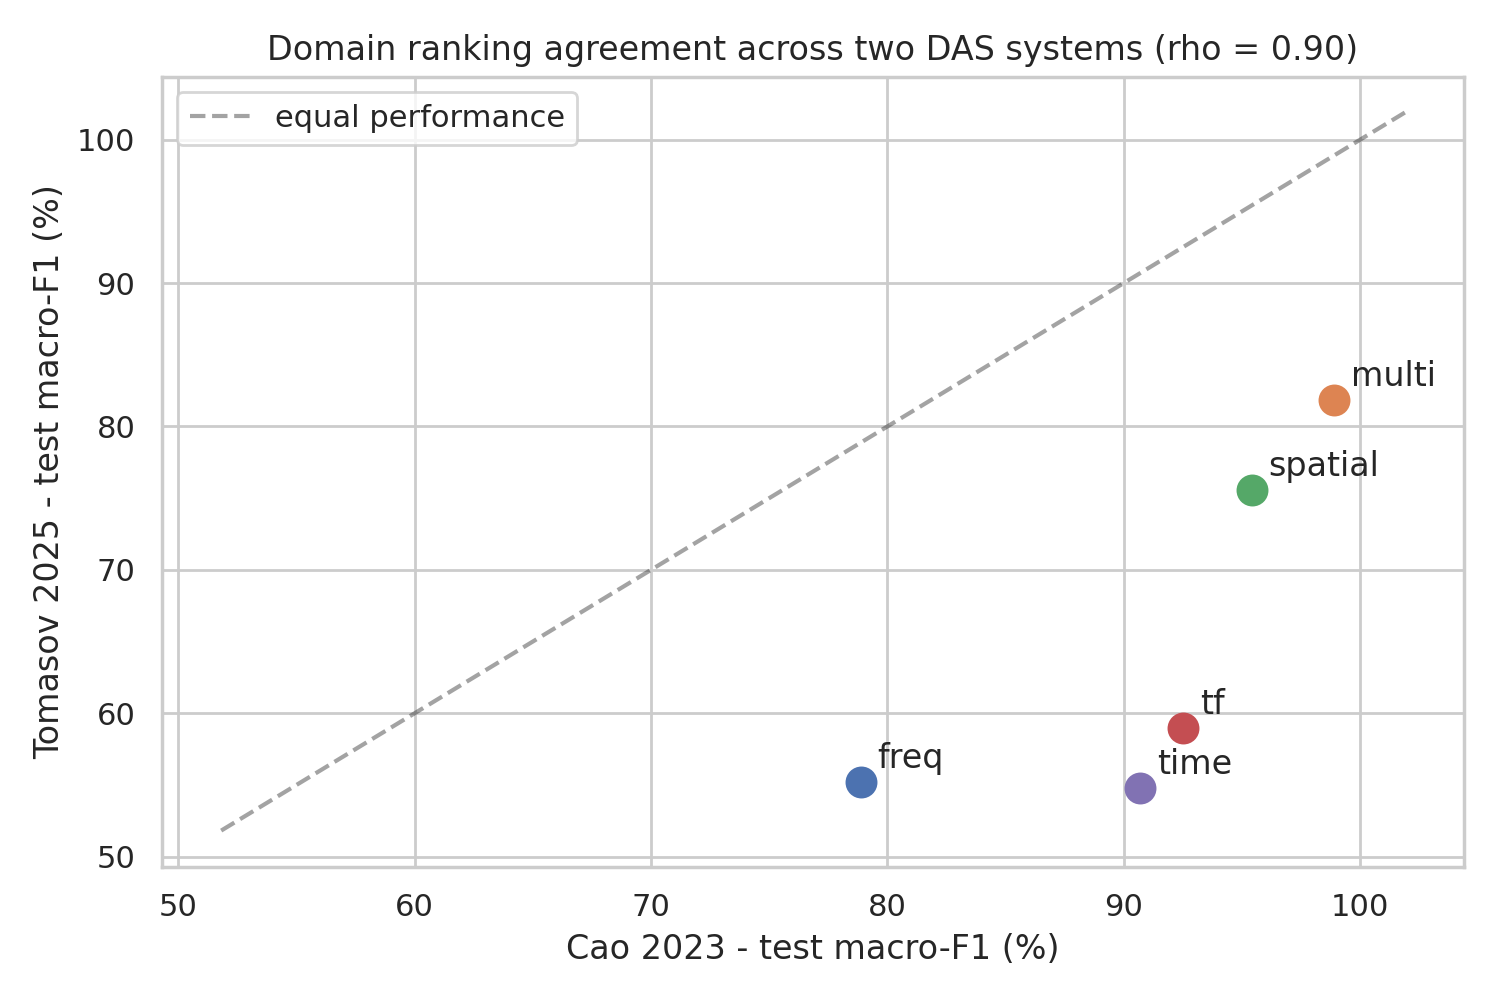
\includegraphics[width=0.75\textwidth,keepaspectratio]{Figures/fig24_domain_agreement.png}
\caption{Agreement in feature-domain performance across the two DAS systems ($\rho = 0.90$).}
\label{fig:domain_agreement}
\end{figure}

\section{Feature Selection}
\label{sec:resSelection}
\autoBookmark{sec}{Feature Selection}
After the group-aware split, \reff{fig:methodology_framework} branches on the feature set: models are trained either on the full fused vector or on the subset retained by the eight-method ensemble, which is fitted on the training set only. The requirement that all eight selectors agree produces compact subsets of 52 of the $1{,}002$ features on Tomasov and 53 on Cao, reductions of $94.8\%$ and $94.7\%$. \reff{fig:consensus_votes} shows the vote distribution on Tomasov and the domain composition of the retained set, and Table~\ref{tab:consensus} gives the composition for both datasets. Time--frequency descriptors constitute $67\%$ and $72\%$ of the two subsets even though that domain is not the strongest in isolation, which indicates that its contribution is complementary rather than redundant.

\begin{figure}[!htbp]
\centering
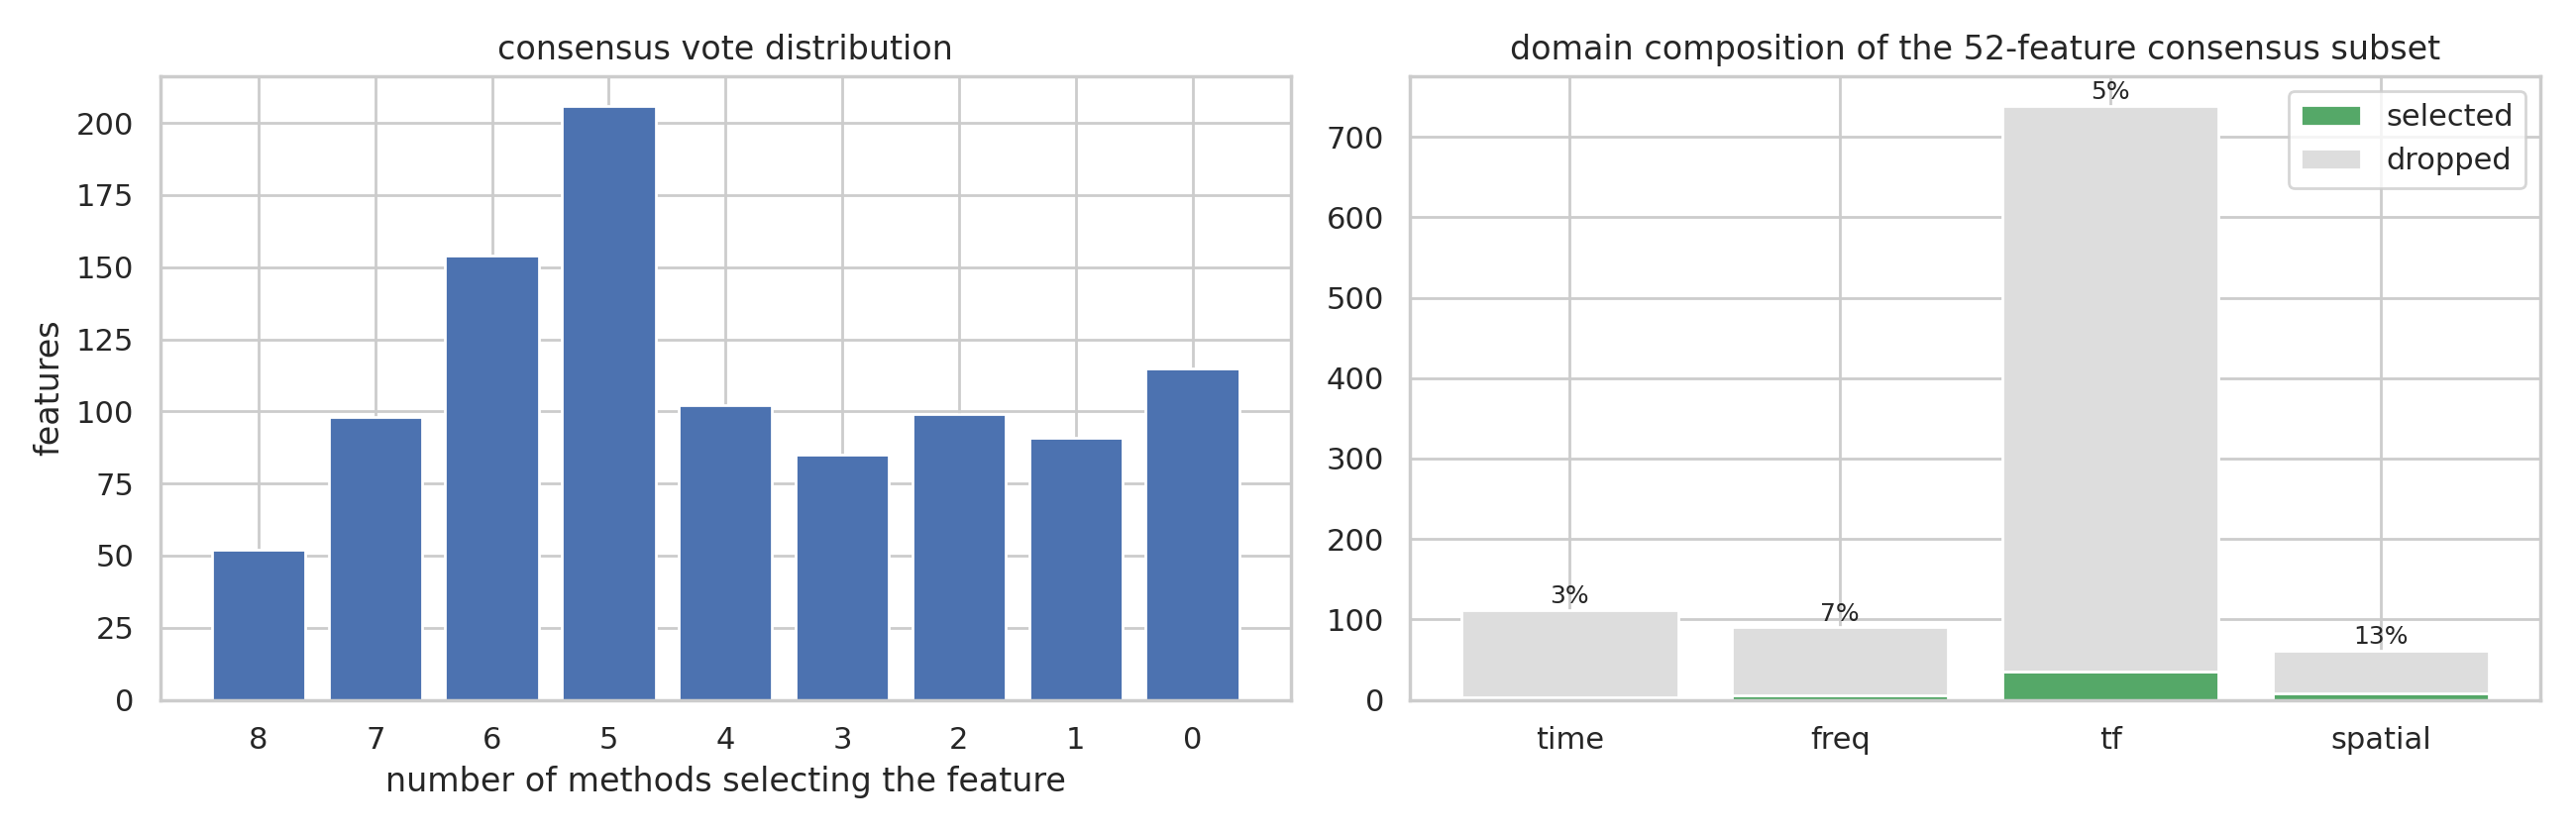
\includegraphics[width=0.95\textwidth,keepaspectratio]{Figures/fig30_consensus_votes_tomasov.png}
\caption{Consensus voting on the Tomasov dataset: number of features selected by $k$ of the eight methods (left) and the domain composition of the 52-feature unanimous subset (right).}
\label{fig:consensus_votes}
\end{figure}

\begin{table}[H]
	\centering
	\caption{Domain composition of the unanimous consensus subsets. Retained is the percentage of that domain's features kept.}
	\label{tab:consensus}
	\small
	\begin{tabular}{@{}lrrrr@{}}
		\toprule
		& \multicolumn{2}{c}{\textbf{Tomasov}} & \multicolumn{2}{c}{\textbf{Cao}}\\
		\cmidrule(lr){2-3}\cmidrule(lr){4-5}
		\textbf{Domain} & \textbf{Selected} & \textbf{Retained} & \textbf{Selected} & \textbf{Retained}\\
		\midrule
		Time            & 3  & 2.7\%  & 12 & 10.7\%\\
		Frequency       & 6  & 6.7\%  & 2  & 2.2\%\\
		Time--frequency & 35 & 4.7\%  & 38 & 5.1\%\\
		Spatial         & 8  & 13.1\% & 1  & 1.6\%\\
		\midrule
		\textbf{Total}  & \textbf{52} & \textbf{5.2\%} & \textbf{53} & \textbf{5.3\%}\\
		\bottomrule
	\end{tabular}
\end{table}

\reff{fig:jaccard} shows the pairwise Jaccard agreement between selectors. Agreement is moderate, and the variance threshold overlaps least with the relevance-based methods, as expected of an unsupervised criterion. This diversity is what makes the unanimity rule meaningful: a feature retained by all eight selectors has simultaneous support from linear correlation, information content, neighbourhood separability, redundancy penalisation, tree importance, and model attribution.

\begin{figure}[!htbp]
\centering
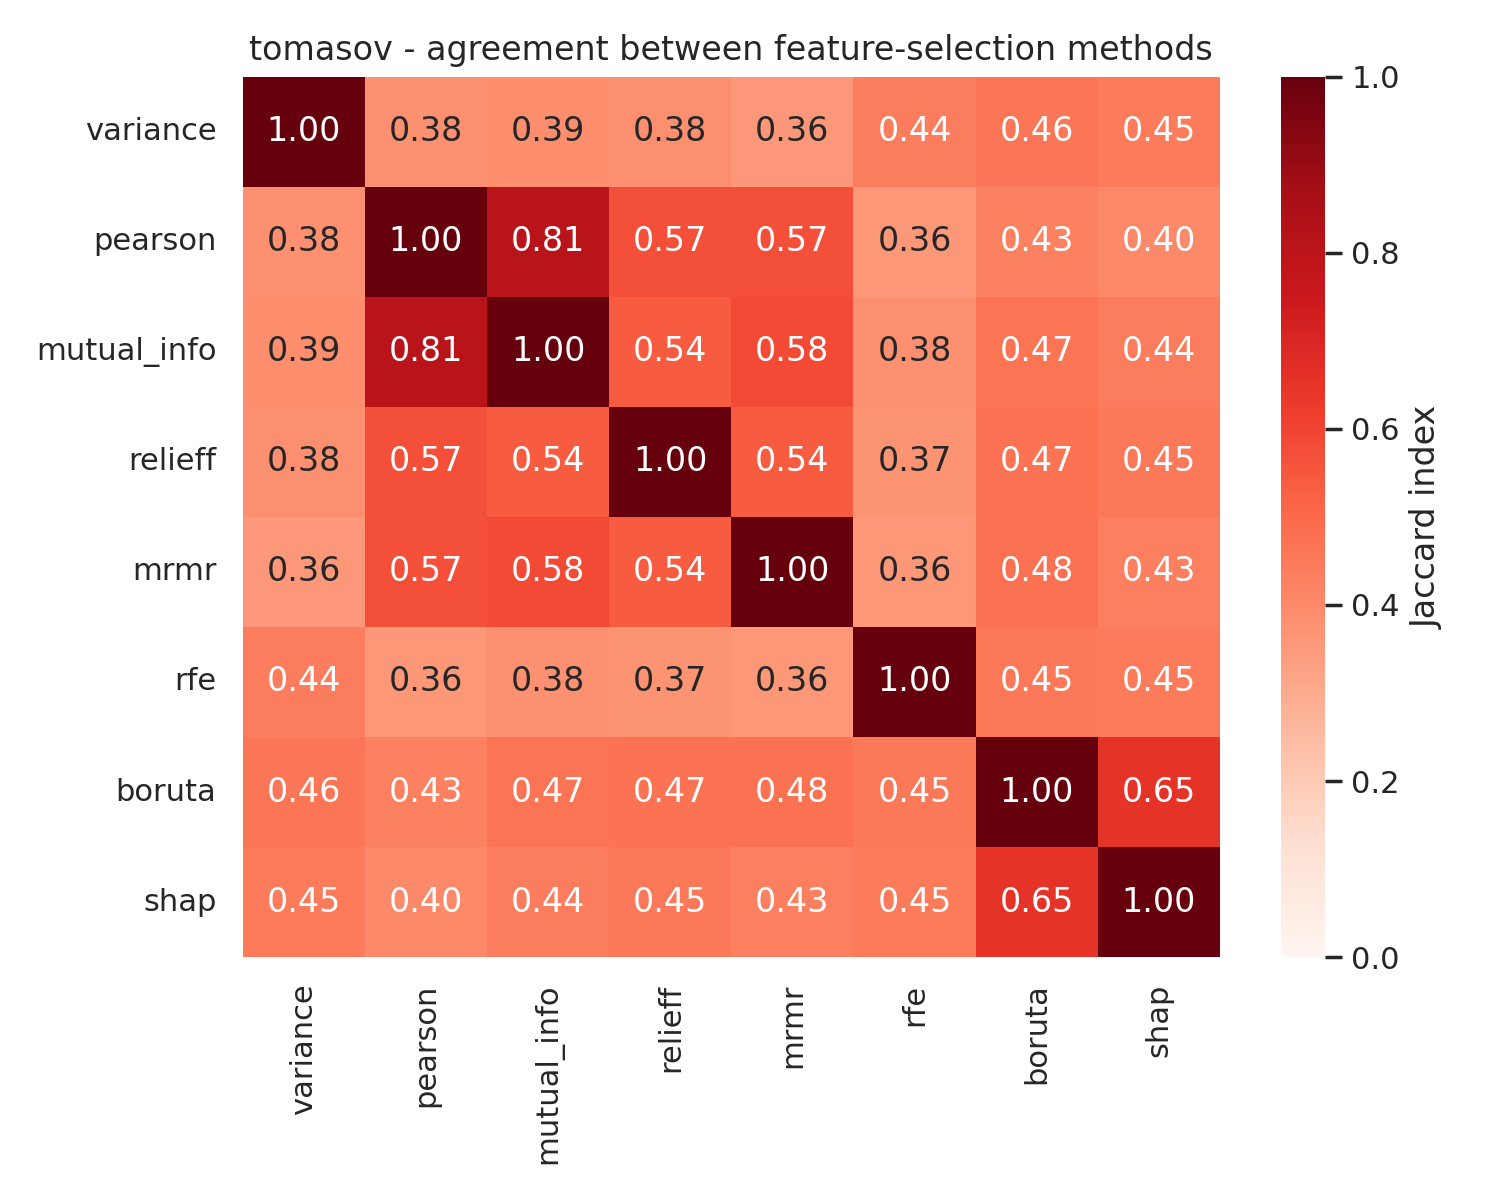
\includegraphics[width=0.48\textwidth,keepaspectratio]{Figures/fig16a_jaccard_tomasov.png}
\hfill
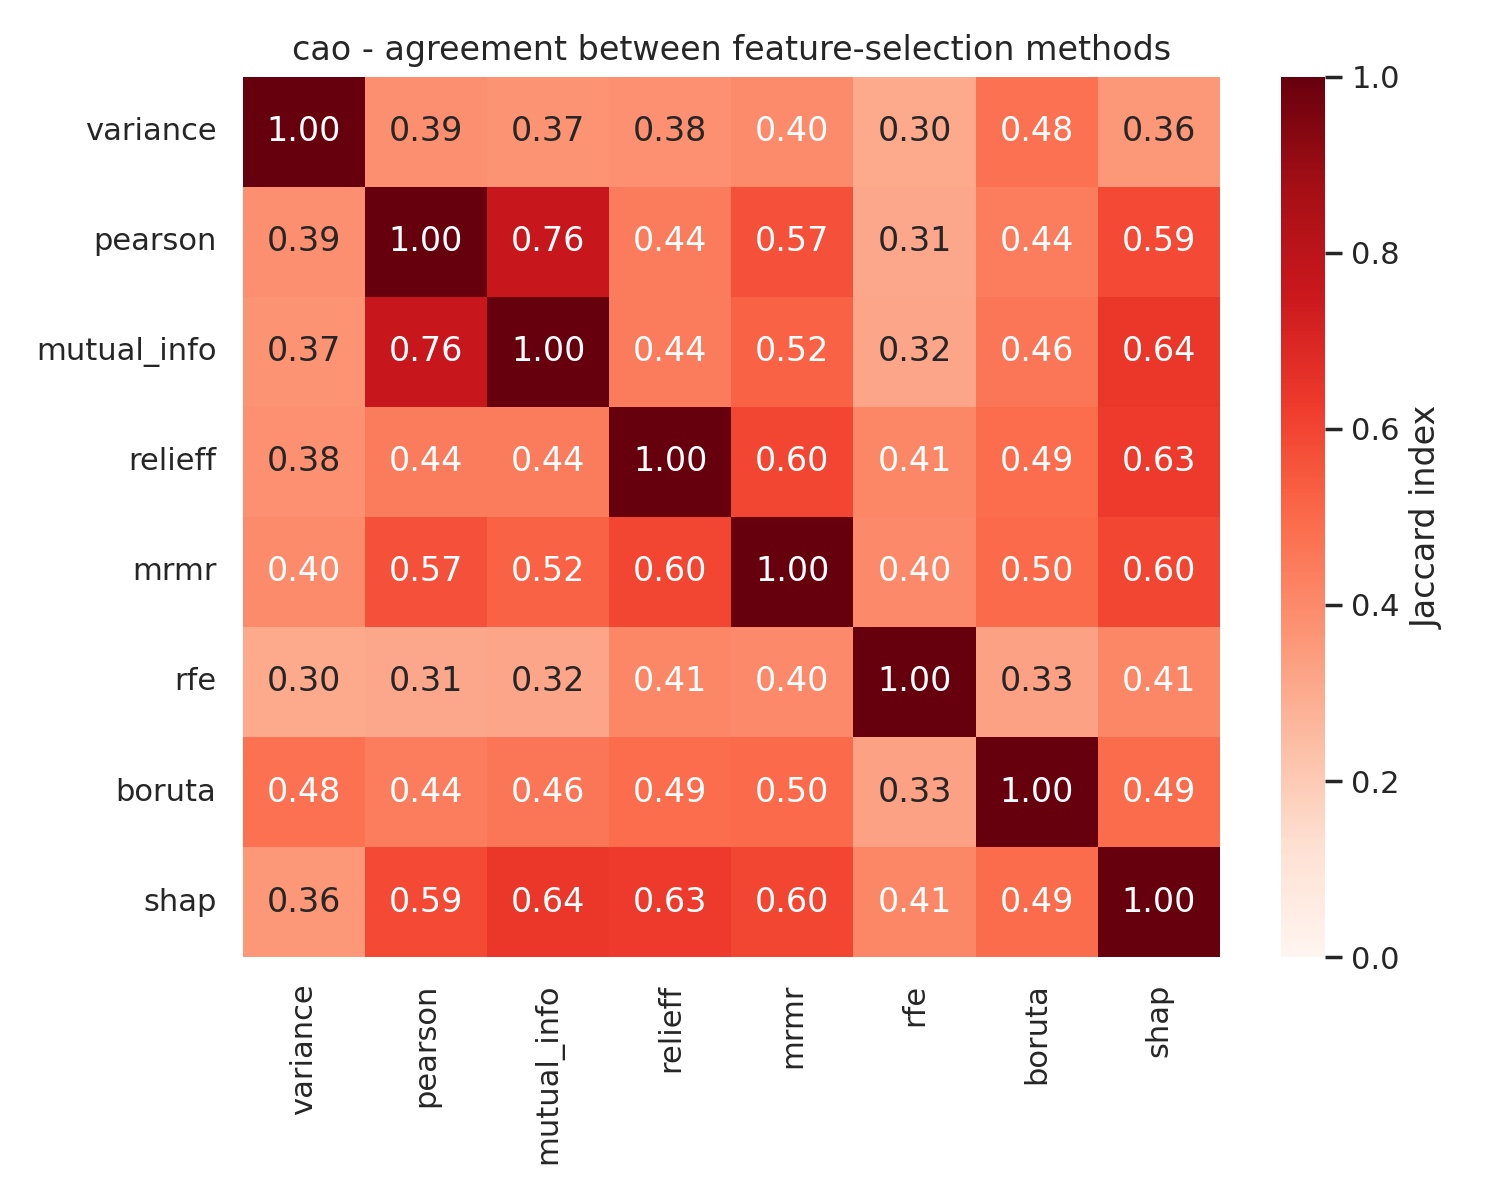
\includegraphics[width=0.48\textwidth,keepaspectratio]{Figures/fig16b_jaccard_cao.png}
\caption{Pairwise Jaccard agreement between the eight feature-selection methods: Tomasov (left) and Cao (right).}
\label{fig:jaccard}
\end{figure}

Compactness is obtained at a cost in accuracy. \reff{fig:reduction} plots validation performance against the number of retained features: the consensus subsets reduce macro-$F_1$ by $8.39$ points on Tomasov ($81.98$ to $73.59$) and by $5.81$ on Cao ($98.90$ to $93.08$). These losses are considerably larger than the sub-point penalty reported in earlier single-dataset work on this benchmark, and they alter the practical recommendation. Unanimous consensus is appropriate when efficiency or interpretability requirements are stringent; otherwise an intermediate operating point on the reduction curve is preferable. This finding answers the feature-selection part of \textbf{RQ2}.

\begin{figure}[!htbp]
\centering
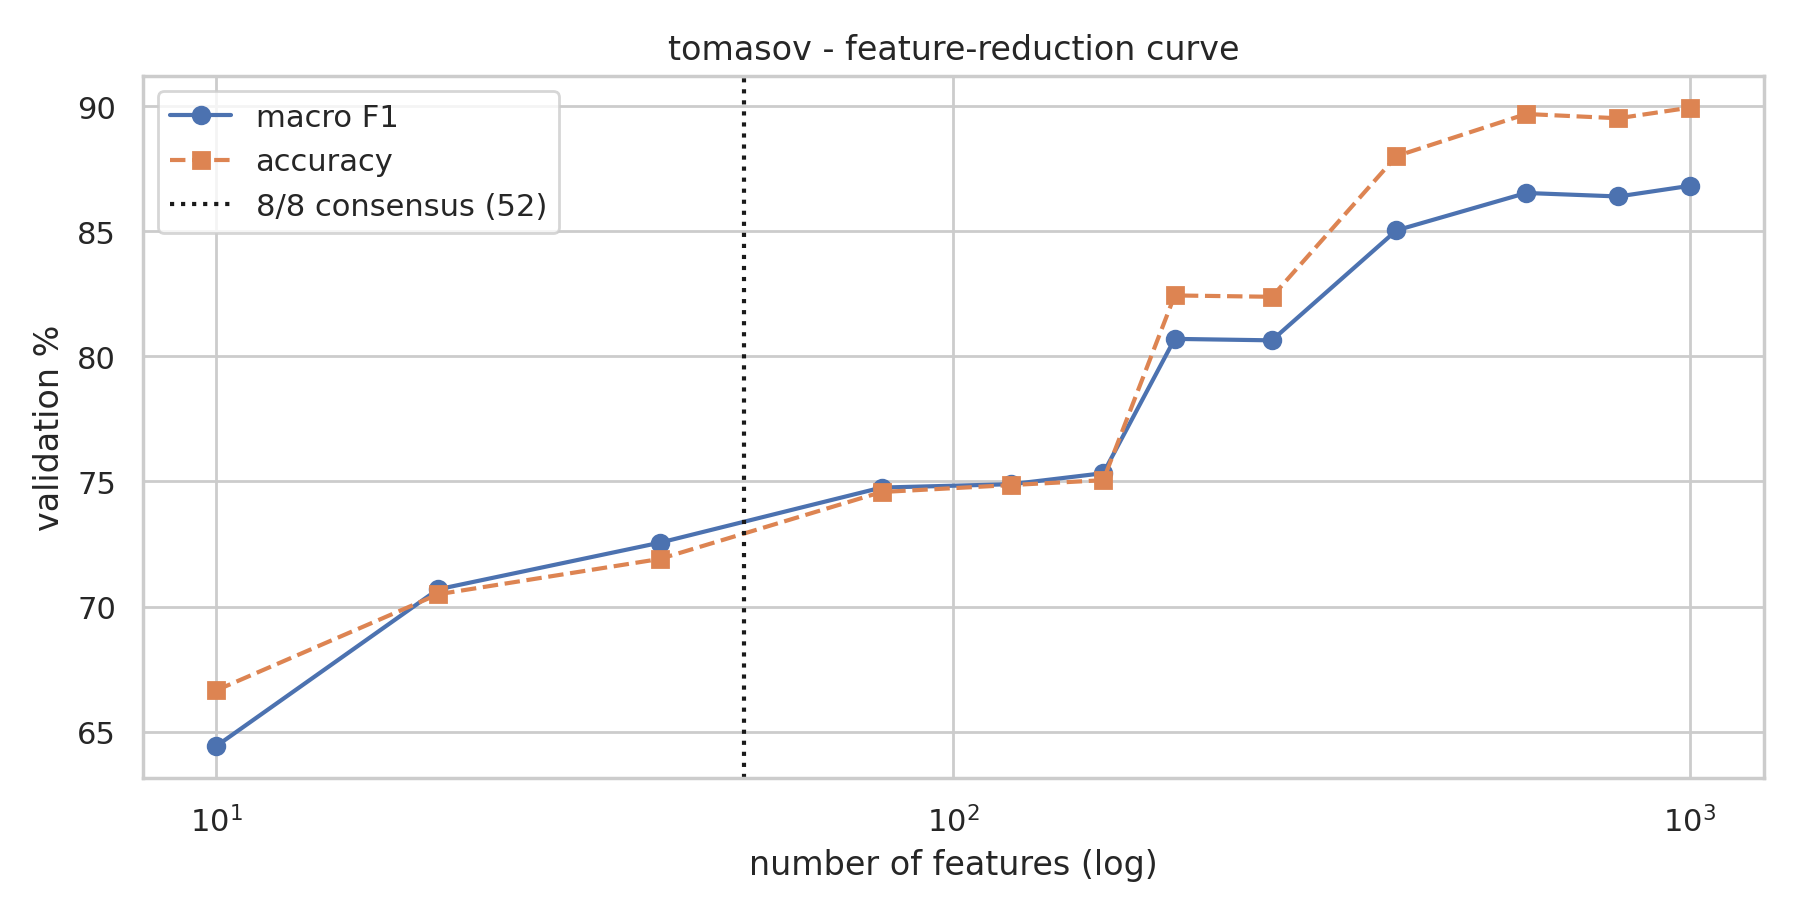
\includegraphics[width=0.48\textwidth,keepaspectratio]{Figures/fig17a_reduction_tomasov.png}
\hfill
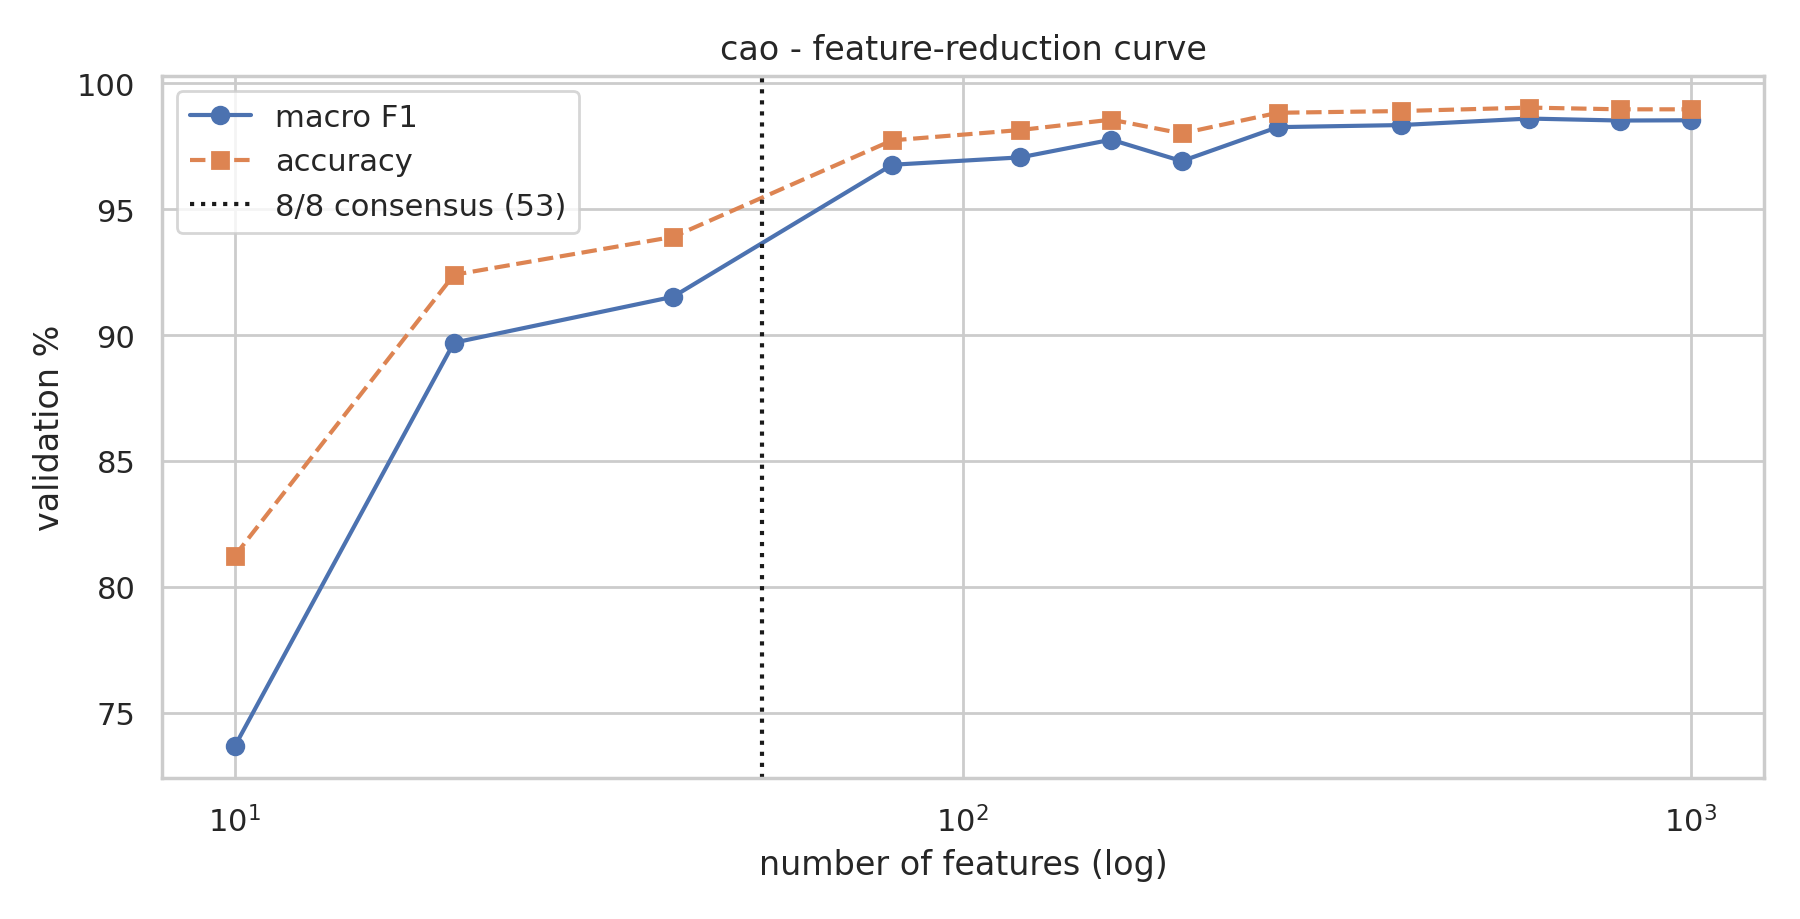
\includegraphics[width=0.48\textwidth,keepaspectratio]{Figures/fig17b_reduction_cao.png}
\caption{Validation performance against the number of retained features: Tomasov (left) and Cao (right).}
\label{fig:reduction}
\end{figure}

\subsection{Lightweight Effect of Feature Selection}
\label{sec:resSelectionLightweight}
\autoBookmark{subsec}{Lightweight Effect of Feature Selection}
\refss{sec:chap3LightweightSelection} identified four respects in which selection can reduce the cost of the pipeline. Table~\ref{tab:selection_footprint} reports each of them for the validation-selected LightGBM configuration on the full and the consensus feature sets. Model size follows the convention of \refss{sec:chap3Efficiency}: stored parameters at 32 bits each.

\begin{table}[!htbp]
	\centering
	\caption{Footprint of the selected LightGBM configuration with the full $1{,}002$-feature vector and with the unanimous consensus subset, on the Jetson AGX Orin. Training and inference run on the CPU. Each configuration uses its own validation-selected balancing strategy, so the training times include different resamplers.}
	\label{tab:selection_footprint}
	\footnotesize
	\setlength{\tabcolsep}{3.5pt}
	\begin{tabular}{@{}lrrrr@{}}
		\toprule
		& \multicolumn{2}{c}{\textbf{Tomasov}} & \multicolumn{2}{c}{\textbf{Cao}}\\
		\cmidrule(lr){2-3}\cmidrule(lr){4-5}
		\textbf{Measure} & \textbf{Full} & \textbf{Consensus} & \textbf{Full} & \textbf{Consensus}\\
		\midrule
		Descriptors per window      & 1{,}002 & 52 & 1{,}002 & 53\\
		Feature vector (bytes)      & 4{,}008 & 208 & 4{,}008 & 212\\
		Fused feature matrix (MB)   & 691.2 & 35.9 & 61.8 & 3.3\\
		Balancing strategy          & Borderline-SMOTE & SMOTE & Undersampling & Borderline-SMOTE\\
		Training time (s)           & 1{,}357.4 & \textbf{63.0} & 41.4 & \textbf{7.9}\\
		Inference (ms per window)   & 0.172 & \textbf{0.145} & \textbf{0.062} & 0.070\\
		Trees                       & 4{,}500 & 4{,}500 & 3{,}000 & 3{,}000\\
		Leaves                      & 288{,}000 & 288{,}000 & 71{,}526 & 121{,}130\\
		Stored parameters           & 855{,}000 & 855{,}000 & 208{,}578 & 357{,}390\\
		Model size, 32-bit (MB)            & 3.42 & 3.42 & \textbf{0.83} & 1.43\\
		Test macro-$F_1$                   & \textbf{81.98} & 73.59 & \textbf{98.90} & 93.08\\
		\bottomrule
	\end{tabular}
\end{table}

Selection substantially reduces the data and training costs of the pipeline. Each window is described by about $95\%$ fewer descriptors; a stored feature vector consequently decreases from $4{,}008$ to approximately 210 bytes and the Tomasov feature store from $691$\,MB to $36$\,MB. Training of the selected model is $21.5$ times faster on Tomasov ($1{,}357$ to $63$\,s) and $5.3$ times faster on Cao ($41$ to $8$\,s), which means that a consensus model can be retrained on the CPU of the embedded board in about one minute when a site or its mix of events changes.

Selection does not, however, make the fitted model smaller or faster to query, and the reason lies in the way in which the size of a boosted ensemble is determined. LightGBM grows one tree per class in each of 500 rounds, with at most 64 leaves per tree, irrespective of the number of input features. On Tomasov every one of the $4{,}500$ trees reaches 64 leaves with either feature set, so both models hold $855{,}000$ parameters ($3.42$\,MB), and inference changes only from $0.172$ to $0.145$\,ms. On Cao the consensus model is the larger of the two ($1.43$ against $0.83$\,MB), because its trees grow more leaves ($121{,}130$ against $71{,}526$), which is consistent with its having been trained on an oversampled rather than an undersampled training set. A smaller model would be obtained by reducing the number of rounds or leaves, not the number of features.

Nor does selection yet reduce the time required for feature extraction, the largest online cost. The extractor computes every domain in full, and the consensus subsets still draw on all four domains (Table~\ref{tab:consensus}), so the reported extraction time of \refs{sec:resEfficiency} applies to both configurations. Computing only the 52 or 53 retained descriptors is the step that would convert the saving in dimensionality into a saving in latency (\refss{sec:chap5FutureCost}).

Selection also incurs a one-time offline cost, $1{,}580$\,s on Tomasov and $1{,}260$\,s on Cao for all eight methods, most of which is attributable to Boruta, and a recurring cost in accuracy of $8.39$ and $5.81$ macro-$F_1$ points. The unanimous subset is therefore the lightweight operating point for storage, transmission, and retraining, the full vector is the operating point for accuracy, and the reduction curve of \reff{fig:reduction} provides the intermediate points between them.

\subsection{Fold-Wise Feature Selection}
\label{sec:resSelectionBias}
\autoBookmark{subsec}{Fold-Wise Feature Selection}
A recurrent criticism of feature-engineering pipelines is that fitting selection once on the training split and then cross-validating on that split inflates the estimate. The controlled comparison of \refss{sec:chap3ConfoundDesign} measured this effect directly by evaluating the identical model on the same grouped folds, once with selection fitted before cross-validation and once with selection refitted in every fold. At this data scale the effect is negligible: the optimism is $+0.02$ points on Tomasov and $-0.19$ on Cao, both within the confidence intervals. With $148{,}229$ and $12{,}155$ training rows, the eight-method consensus is sufficiently stable that its position relative to the fold boundary does not measurably change the estimate. Fold-wise selection remains the correct practice, particularly for smaller datasets, but in this setting the optimism of earlier results is attributable to partition leakage rather than to the placement of feature selection.

\section{Training Set Balancing Strategies}
\label{sec:resBalancing}
\autoBookmark{sec}{Training Set Balancing Strategies}
Each of the six balancing strategies is applied to the training set alone, after feature selection and immediately before modelling, which leaves the validation and test distributions unaltered. \reff{fig:heatmaps} shows the validation macro-$F_1$ for every (classifier, strategy) pair, and two patterns are evident. The gradient-boosting family occupies the top three rows on both datasets by a clear margin, and within any row the six columns differ by a fraction of that margin. Averaged over the seven classifiers, the range of test macro-$F_1$ across strategies is $1.94$ points on Tomasov and $0.44$ on Cao, the former well within the $\pm 4.42$-point partition standard deviation reported in \refs{sec:resStats}. Validation selects Borderline-SMOTE for Tomasov and random undersampling for Cao, but the second- and third-ranked strategies are lower by only a few tenths of a point.

\begin{figure}[!htbp]
\centering
\begin{subfigure}[b]{0.49\textwidth}
	\centering
	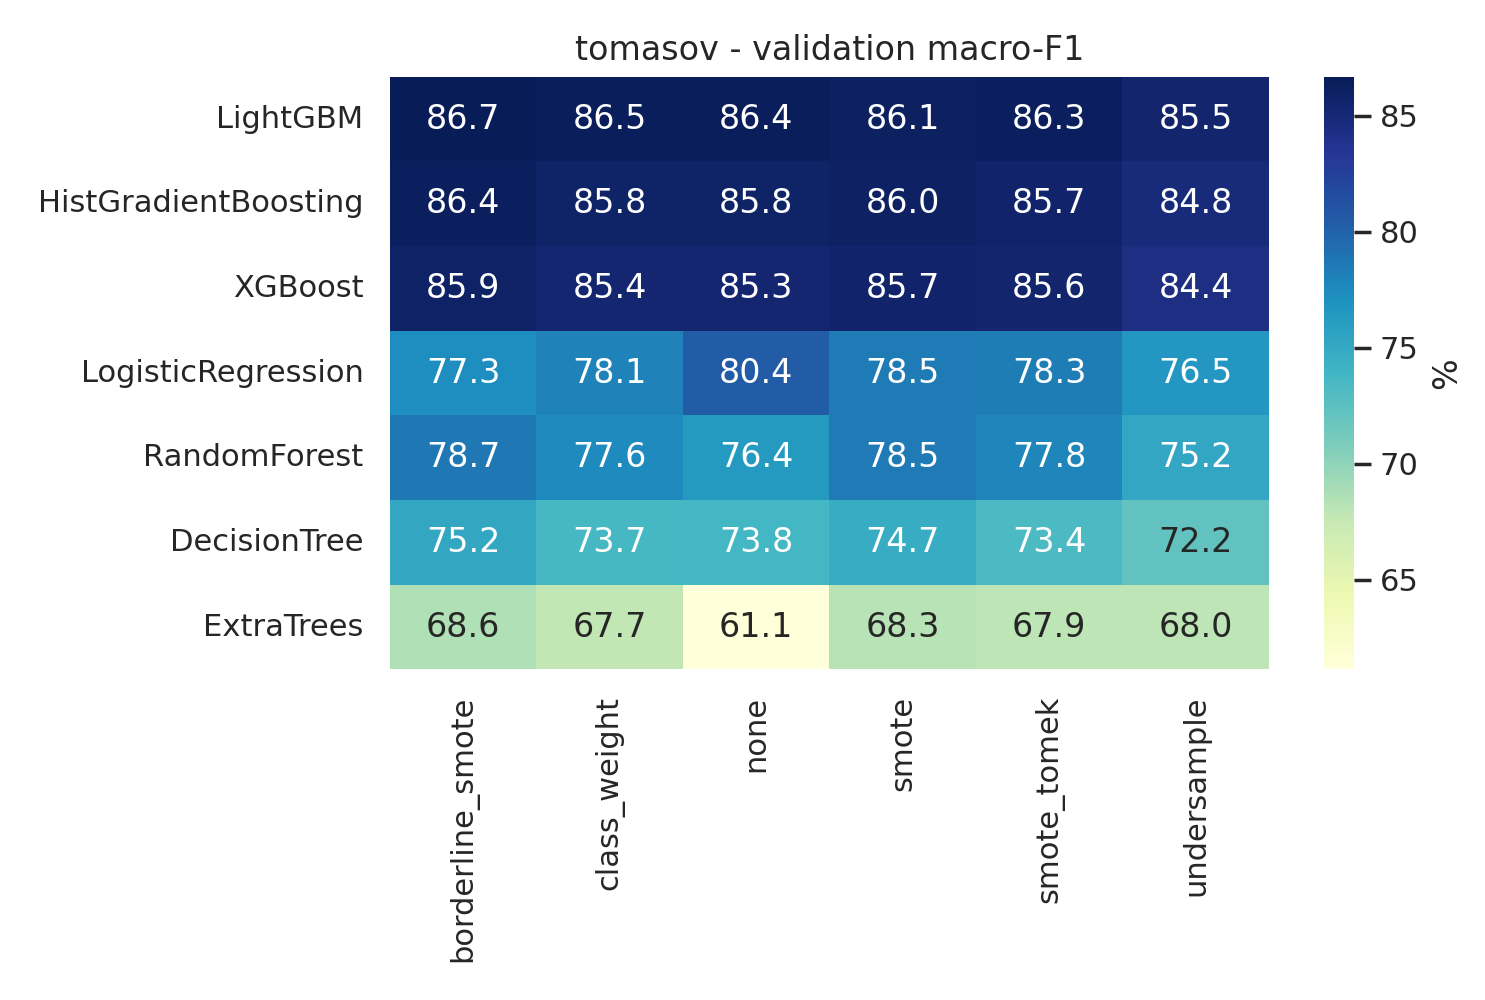
\includegraphics[width=\textwidth,keepaspectratio]{Figures/fig29a_heatmap_tomasov.png}
	\caption{Tomasov 2025}
\end{subfigure}\hfill
\begin{subfigure}[b]{0.49\textwidth}
	\centering
	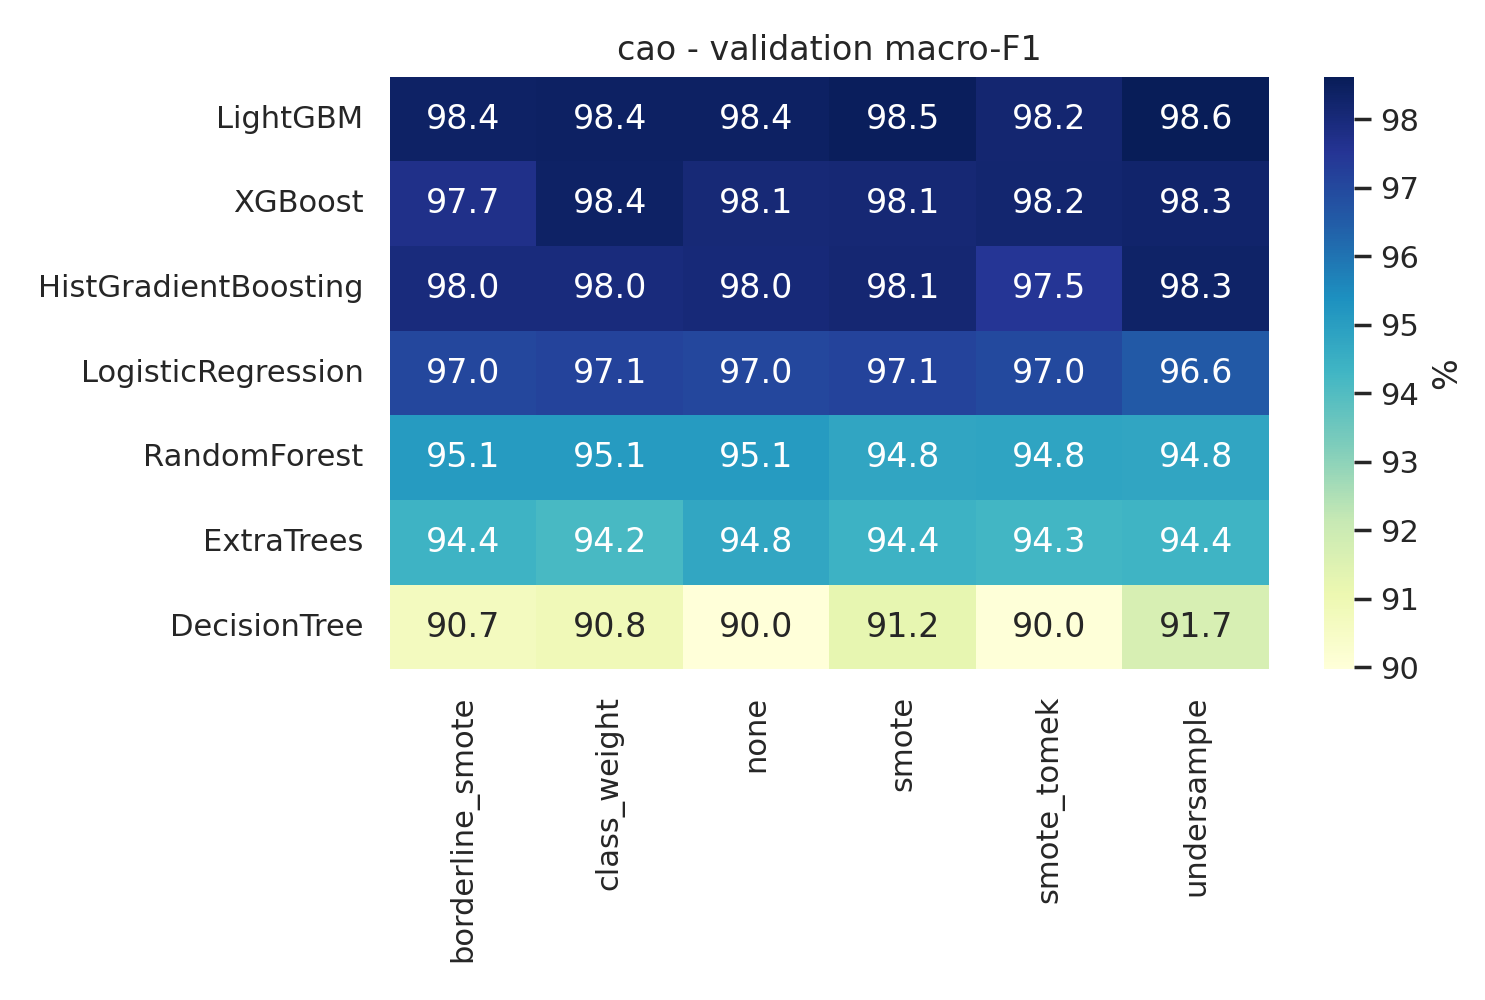
\includegraphics[width=\textwidth,keepaspectratio]{Figures/fig29b_heatmap_cao.png}
	\caption{Cao 2023}
\end{subfigure}
\caption{Validation macro-$F_1$ (\%) for every classifier and balancing strategy on the full $1{,}002$-feature representation. Rows are ordered by mean performance.}
\label{fig:heatmaps}
\end{figure}

These results do not support a consistent advantage for cost-sensitive class weighting. When the strategies are compared over independent held-out acquisitions (\refs{sec:resStats}), two pairs can be distinguished on Tomasov, by a margin that reflects recall on single-class recordings rather than general classification quality, and no pair can be distinguished on Cao. Computational cost is therefore the more useful criterion. Class weighting and the no-balancing baseline both avoid the synthetic-sample generation and training-set inflation of the SMOTE family, which on Tomasov approximately doubles the fitting time ($1{,}756$\,s for Borderline-SMOTE against $798$\,s for class weighting) without a reliable gain. This result answers the class-balancing part of \textbf{RQ2}; together with \refs{sec:resDomains} and \refs{sec:resSelection} it establishes the representation and training components, and \refs{sec:resFinal} adds the choice of classifier.

\section{Modelling}
\label{sec:resFinal}
\autoBookmark{sec}{Modelling}
The modelling stage of \reff{fig:methodology_framework} trains seven classifiers on every combination of feature set and balancing strategy and uses the validation set to choose among them. Each classifier is represented by the balancing strategy that maximised its own validation macro-$F_1$, which yields one configuration per classifier chosen by the same rule, and the configuration with the highest validation macro-$F_1$ across classifiers is the selected model. \refss{sec:resAllModels} compares the seven classifiers on effectiveness and cost, and \refss{sec:resSelected} reports the selected configuration and its generalisation gap. \refs{sec:resPerformance} then examines the per-class behaviour of all seven.

\subsection{Classifier Comparison}
\label{sec:resAllModels}
\autoBookmark{subsec}{Classifier Comparison}
Table~\ref{tab:all_models} reports the seven classifiers on both datasets, on each of which they form the same three tiers. The gradient-boosting family (LightGBM, XGBoost, and histogram-based gradient boosting) occupies the top three positions, and its members lie within $0.62$ macro-$F_1$ points of one another on Tomasov and $0.84$ on Cao. Logistic regression forms a second tier, $3.38$ points behind LightGBM on Tomasov but only $1.06$ behind on Cao. The bagged ensembles and the single decision tree form the third tier. The best and worst classifiers differ by $14.32$ points on Tomasov and $7.34$ on Cao; the choice of learner is thus about twice as consequential on the more difficult dataset.

\begin{table}[!htbp]
	\centering
	\caption{All seven classifiers on the full $1{,}002$-feature representation, each at the balancing strategy that maximised its own validation macro-$F_1$, ordered by validation macro-$F_1$. Test metrics in \%. The consensus column gives test macro-$F_1$ on the unanimous subset, again at each classifier's own validation-selected strategy. Times are from the benchmark run on the Jetson AGX Orin and can differ slightly from the final-model timings of Table~\ref{tab:main_results}.}
	\label{tab:all_models}
	\footnotesize
	\setlength{\tabcolsep}{3pt}
	\resizebox{\textwidth}{!}{%
	\begin{tabular}{@{}llrrrrrrrr@{}}
		\toprule
		\textbf{Classifier} & \textbf{Balancing} & \textbf{Val.\ $F_1$} & \textbf{Acc.} & \textbf{Bal.\ acc.} & \textbf{Macro-$F_1$} & \textbf{AUC} & \textbf{Train (s)} & \textbf{Infer.\ (ms)} & \textbf{Consensus $F_1$}\\
		\midrule
		\multicolumn{10}{@{}l}{\textit{Tomasov \etal\ 2025 (9 classes)}}\\[2pt]
		LightGBM             & Borderline-SMOTE & \textbf{86.69} & \textbf{90.71} & \textbf{81.97} & 81.98 & 97.46 & 1{,}393.1 & 0.183  & 73.59\\
		HistGradientBoosting & Borderline-SMOTE & 86.35 & 90.50 & 81.96 & \textbf{82.12} & \textbf{97.52} & 1{,}880.7 & 0.223  & 73.19\\
		XGBoost              & Borderline-SMOTE & 85.93 & 90.37 & 81.60 & 81.50 & 96.45 & 4{,}285.6 & 0.046  & \textbf{73.68}\\
		LogisticRegression   & None             & 80.41 & 84.38 & 77.68 & 78.59 & 96.95 & 1{,}070.6 & 0.011  & 67.76\\
		RandomForest         & Borderline-SMOTE & 78.67 & 82.72 & 75.63 & 75.63 & 94.66 & 914.7     & 0.030  & 72.09\\
		DecisionTree         & Borderline-SMOTE & 75.16 & 79.83 & 70.96 & 71.69 & 87.49 & 1{,}039.7 & 0.001  & 64.27\\
		ExtraTrees           & Borderline-SMOTE & 68.60 & 72.38 & 68.72 & 67.80 & 93.31 & 398.0     & 0.034  & 66.92\\
		\midrule
		\multicolumn{10}{@{}l}{\textit{Cao \etal\ 2023 (6 classes)}}\\[2pt]
		LightGBM             & Undersampling    & \textbf{98.62} & \textbf{99.06} & \textbf{98.98} & \textbf{98.90} & \textbf{99.99} & 40.2      & 0.067  & \textbf{93.08}\\
		XGBoost              & Class weighting  & 98.36 & 98.61 & 98.54 & 98.38 & 99.98 & 173.4     & 0.012  & 92.53\\
		HistGradientBoosting & Undersampling    & 98.32 & 98.45 & 98.13 & 98.06 & 99.96 & 44.5      & 0.019  & 92.17\\
		LogisticRegression   & Class weighting  & 97.14 & 98.23 & 98.16 & 97.84 & 99.96 & 8.6       & 0.025  & 88.09\\
		RandomForest         & None             & 95.08 & 97.50 & 97.58 & 97.21 & 99.90 & 12.6      & 0.074  & 91.50\\
		ExtraTrees           & None             & 94.76 & 97.00 & 96.95 & 96.51 & 99.89 & 3.9       & 0.079  & 91.20\\
		DecisionTree         & Undersampling    & 91.68 & 92.73 & 92.30 & 91.56 & 94.97 & 16.8      & 0.001  & 84.74\\
		\bottomrule
	\end{tabular}}
\end{table}

The validation rule selects LightGBM in all four combinations of dataset and feature set, but the test ordering within the boosting tier does not always agree with it. On the full Tomasov representation, histogram-based gradient boosting reaches a test macro-$F_1$ of $82.12$ against $81.98$ for LightGBM, and on the Tomasov consensus subset XGBoost reaches $73.68$ against $73.59$. These reversals of $0.14$ and $0.09$ points are a small fraction of the $\pm 4.42$-point partition standard deviation on Tomasov (\refs{sec:resStats}), so the three boosted learners cannot be distinguished on these data. The defensible conclusion for the development of the pipeline (\textbf{RQ2}) is therefore that it performs best with a gradient-boosting learner, with LightGBM as the member selected by the validation rule rather than a member shown to outperform the other two.

Logistic regression performs better than its linear form might suggest. On Cao it is only $1.06$ points below LightGBM while training in $8.6$\,s, which indicates that the fused descriptors render the six Cao classes close to linearly separable. It is, however, the learner that depends most strongly on the full representation: the consensus subsets reduce its score by $10.83$ points on Tomasov and $9.75$ on Cao, compared with $8.39$ and $5.81$ for LightGBM, which is consistent with a linear model that combines many weakly informative features that the unanimity rule discards. The bagged ensembles exhibit the opposite pattern. On the full Tomasov representation, extremely randomised trees fall below the single decision tree in macro-$F_1$ ($67.80$ against $71.69$) despite a higher one-vs-rest AUC ($93.31$ against $87.49$), which indicates that their probability rankings separate the classes better than their decisions do. On the 52-feature consensus subset the same model loses only $0.88$ points and random forest only $3.54$, against $8.39$ for LightGBM. Both observations indicate dilution by uninformative columns. The bagged ensembles consider only 31 randomly drawn features at each split, the square root of $1{,}002$, so on the full representation many candidate splits involve no informative feature, whereas the boosted learners search at least $80\%$ of the features at every split and are largely unaffected. The weaker learners are also more sensitive to the balancing strategy: across the six strategies, test macro-$F_1$ varies by $6.66$ points for extremely randomised trees on Tomasov but by only $0.63$ for LightGBM.

Within the top tier, computational cost distinguishes the classifiers more clearly than effectiveness does. On Tomasov, XGBoost requires $4{,}286$\,s to train compared with $1{,}393$\,s for LightGBM but predicts a window in $0.046$\,ms rather than $0.183$\,ms, and histogram-based gradient boosting is the slowest of the three at prediction. Every classifier predicts a window in well under a millisecond on the CPU of the Jetson AGX Orin, between two and five orders of magnitude below the window-arrival intervals of $102.4$\,ms (Tomasov) and $204.8$\,ms (Cao). Inference cost therefore does not discriminate between the learners in deployment; training cost does, and, as \refs{sec:resEfficiency} shows, so does feature extraction.

\subsection{Selection on the Validation Set}
\label{sec:resSelected}
\autoBookmark{subsec}{Selection on the Validation Set}
Table~\ref{tab:main_results} reports the configuration selected on validation for each dataset and feature set. LightGBM is selected in all four cases, subject to the qualification stated above, and this selected configuration is the one compared with the published and recent baselines in the Discussion (\refs{sec:resDiscussion}). With the full feature set it reaches $90.71\%$ accuracy and $81.98$ macro-$F_1$ on the nine-class Tomasov dataset and $99.06\%$ accuracy and $98.90$ macro-$F_1$ on the six-class Cao dataset, with inference below $0.2$\,ms per window. The pipeline designed on the primary dataset is thus applied unchanged to the evaluation dataset, with the same settings and without per-dataset tuning, which completes the development required by \textbf{RQ2}.

\begin{table}[!htbp]
	\centering
	\caption{Final results under the leakage-controlled protocol, measuring segment-level generalisation within represented recordings. Model and balancing strategy selected on validation; test metrics reported once.}
	\label{tab:main_results}
	\footnotesize
	\setlength{\tabcolsep}{3.5pt}
	\resizebox{\textwidth}{!}{%
\begin{tabular}{@{}lllrrrrrr@{}}
		\toprule
		\textbf{Dataset} & \textbf{Feature set} & \textbf{Balancing} & \textbf{Feat.} & \textbf{Acc. (\%)} & \textbf{Bal. acc.} & \textbf{Macro-$F_1$} & \textbf{CV $F_1$} & \textbf{Infer. (ms)}\\
		\midrule
		Tomasov (9 cls) & Multi-domain  & Borderline-SMOTE & 1{,}002 & \textbf{90.71} & \textbf{81.97} & \textbf{81.98} & 78.60 & 0.172\\
		Tomasov (9 cls) & Consensus 8/8 & SMOTE            & 52      & 77.29          & 72.88          & 73.59          & 66.25 & 0.145\\
		Cao (6 cls)     & Multi-domain  & Undersampling    & 1{,}002 & \textbf{99.06} & \textbf{98.98} & \textbf{98.90} & 98.51 & 0.062\\
		Cao (6 cls)     & Consensus 8/8 & Borderline-SMOTE & 53      & 94.40          & 93.36          & 93.08          & 93.93 & 0.070\\
		\bottomrule
	\end{tabular}}
\end{table}

For the full feature set, the held-out test macro-$F_1$ exceeds the cross-validated estimate by $3.38$ points on Tomasov and $0.38$ on Cao, which indicates that the $1{,}002$-dimensional representation does not overfit substantially; the larger Tomasov gap is consistent with the greater heterogeneity of its recordings. These figures measure generalisation to unseen segments of recordings that are represented in training. \refs{sec:resGeneralisation} reports the cross-recording measurement, which is available for the four Tomasov classes recorded more than once and yields $63.85\%$ accuracy. The figures also retain the numerical residue in the normalisation that a subsequent audit of the feature code identified; \refss{sec:chap5LimResidue} reports its magnitude, which is substantial on Tomasov and small on Cao.

\section{Performance Evaluation}
\label{sec:resPerformance}
\autoBookmark{sec}{Performance Evaluation}
The performance evaluation stage of \reff{fig:methodology_framework} scores every model with accuracy, precision, recall, and $F_1$ on the same test windows. \refs{sec:resFinal} compared the seven classifiers on aggregate metrics, and the Discussion (\refs{sec:resDiscussion}) compares them with the models of the baseline branch. This section examines per-class behaviour, in which the differences between learners and the limits of the representation become apparent. \refss{sec:resPerClass} reports the per-class $F_1$ of all seven classifiers, \refss{sec:resOpenclose} examines the class that no feature-based classifier recovers, and \refss{sec:resErrors} examines the remaining dominant error mode.

\subsection{Per-Class Performance}
\label{sec:resPerClass}
\autoBookmark{subsec}{Per-Class Performance}
Table~\ref{tab:per_class} gives the test $F_1$ of every class for all seven classifiers, and \reff{fig:confusion_tomasov} and \reff{fig:confusion_cao} show the confusion matrices of the selected LightGBM configuration. The per-class values were obtained by retraining each classifier at its validation-selected strategy on the frozen partition. The retrained models match the benchmark of Table~\ref{tab:all_models} to the second decimal place for every classifier except two, and in neither case is the difference sufficient to alter a comparison: logistic regression on Tomasov, whose L-BFGS solver stops at its iteration limit before formal convergence, differs by $0.16$ macro-$F_1$ points, and XGBoost differs by $0.14$ on Tomasov and by less than $0.01$ on Cao.

\begin{table}[!htbp]
	\centering
	\caption{Per-class test $F_1$ of all seven classifiers on the full $1{,}002$-feature representation, each at its validation-selected balancing strategy. The best value in each row is in bold; $n$ is the test support. LGBM: LightGBM; XGB: XGBoost; HGB: histogram-based gradient boosting; LR: logistic regression; RF: random forest; ET: extremely randomised trees; DT: decision tree.}
	\label{tab:per_class}
	\footnotesize
	\setlength{\tabcolsep}{4pt}
	\begin{tabular}{@{}lrrrrrrrr@{}}
		\toprule
		\textbf{Class} & \textbf{$n$} & \textbf{LGBM} & \textbf{XGB} & \textbf{HGB} & \textbf{LR} & \textbf{RF} & \textbf{ET} & \textbf{DT}\\
		\midrule
		\multicolumn{9}{@{}l}{\textit{Tomasov \etal\ 2025}}\\[2pt]
		Car           &   1{,}772 & 0.845 & 0.831 & \textbf{0.846} & 0.728 & 0.729 & 0.581 & 0.751\\
		Construction  &   2{,}232 & \textbf{0.996} & 0.994 & 0.995 & 0.971 & 0.963 & 0.929 & 0.969\\
		Fence         &   1{,}983 & \textbf{0.893} & 0.889 & 0.889 & 0.769 & 0.731 & 0.505 & 0.804\\
		Longboard     &       581 & 0.912 & 0.913 & 0.906 & 0.910 & \textbf{0.933} & 0.887 & 0.736\\
		Manipulation  &       867 & \textbf{0.993} & 0.986 & \textbf{0.993} & 0.967 & 0.935 & 0.881 & 0.817\\
		Openclose     &       198 & 0.044 & 0.018 & 0.074 & \textbf{0.189} & 0.000 & 0.035 & 0.042\\
		Regular       &   1{,}111 & 0.847 & \textbf{0.849} & 0.844 & 0.738 & 0.705 & 0.566 & 0.757\\
		Running       &       929 & 0.946 & \textbf{0.948} & 0.944 & 0.945 & 0.947 & 0.933 & 0.787\\
		Walk          &   1{,}661 & \textbf{0.903} & 0.897 & 0.900 & 0.871 & 0.863 & 0.784 & 0.790\\
		\midrule
		\multicolumn{9}{@{}l}{\textit{Cao \etal\ 2023}}\\[2pt]
		Background    &       227 & \textbf{0.996} & \textbf{0.996} & \textbf{0.996} & 0.989 & 0.987 & 0.983 & 0.965\\
		Digging       &       370 & \textbf{0.988} & 0.987 & \textbf{0.988} & 0.985 & 0.967 & 0.973 & 0.911\\
		Knocking      &       622 & \textbf{0.998} & 0.995 & 0.995 & 0.990 & 0.986 & 0.982 & 0.968\\
		Shaking       &       134 & \textbf{0.993} & 0.978 & 0.978 & 0.960 & 0.968 & 0.950 & 0.901\\
		Walking       &       232 & \textbf{0.976} & 0.963 & 0.955 & 0.969 & 0.950 & 0.938 & 0.847\\
		Watering      &       218 & \textbf{0.984} & \textbf{0.984} & 0.972 & 0.977 & 0.975 & 0.965 & 0.901\\
		\bottomrule
	\end{tabular}
\end{table}

The Tomasov dataset differentiates the learners far more than the Cao dataset does, and the per-class pattern shows where the differences arise. The boosted learners lead on seven of the nine classes, and that lead is shared among all three: LightGBM is best on four classes, XGBoost on two, and histogram-based gradient boosting on one, which is consistent with the conclusion of \refss{sec:resAllModels} that the three cannot be distinguished. Random forest is best on \emph{longboard} ($0.933$), and logistic regression is best on \emph{openclose}, although only at $0.189$. The learners differ most on \emph{fence}, \emph{regular}, and \emph{car}, with spreads of $0.388$, $0.282$, and $0.265$, and these are the three classes involved in the dominant confusions examined below. Three of the five single-recording classes, \emph{construction}, \emph{manipulation}, and \emph{running}, reach at least $0.88$ for every learner except the single decision tree; as \refs{sec:resConfound} shows, high scores on such classes cannot be separated from recognition of the recording itself. Table~\ref{tab:error_modes} traces the two dominant error modes across all seven learners, and both occur in every one of them.

On Cao the ranking of the classes is almost identical for every learner. The three boosted learners exceed an $F_1$ of $0.95$ on every class, and \emph{walking} is the weakest class for six of the seven classifiers, ranging from $0.847$ for the decision tree to $0.976$ for LightGBM. Its errors are assigned mainly to \emph{digging}, which receives between $1.3\%$ (LightGBM) and $6.9\%$ (decision tree) of the walking windows. Logistic regression is the exception: it misclassifies only $0.4\%$ of the walking windows in this way, and its weakest class is \emph{shaking} at $0.960$. The spread between the best and worst learner is smallest for \emph{background} and \emph{knocking} ($0.030$) and largest for \emph{walking} ($0.129$); the learners thus differ most on the class whose signature overlaps with those of other classes and least on the classes with distinctive signatures.

\begin{figure}[!htbp]
\centering
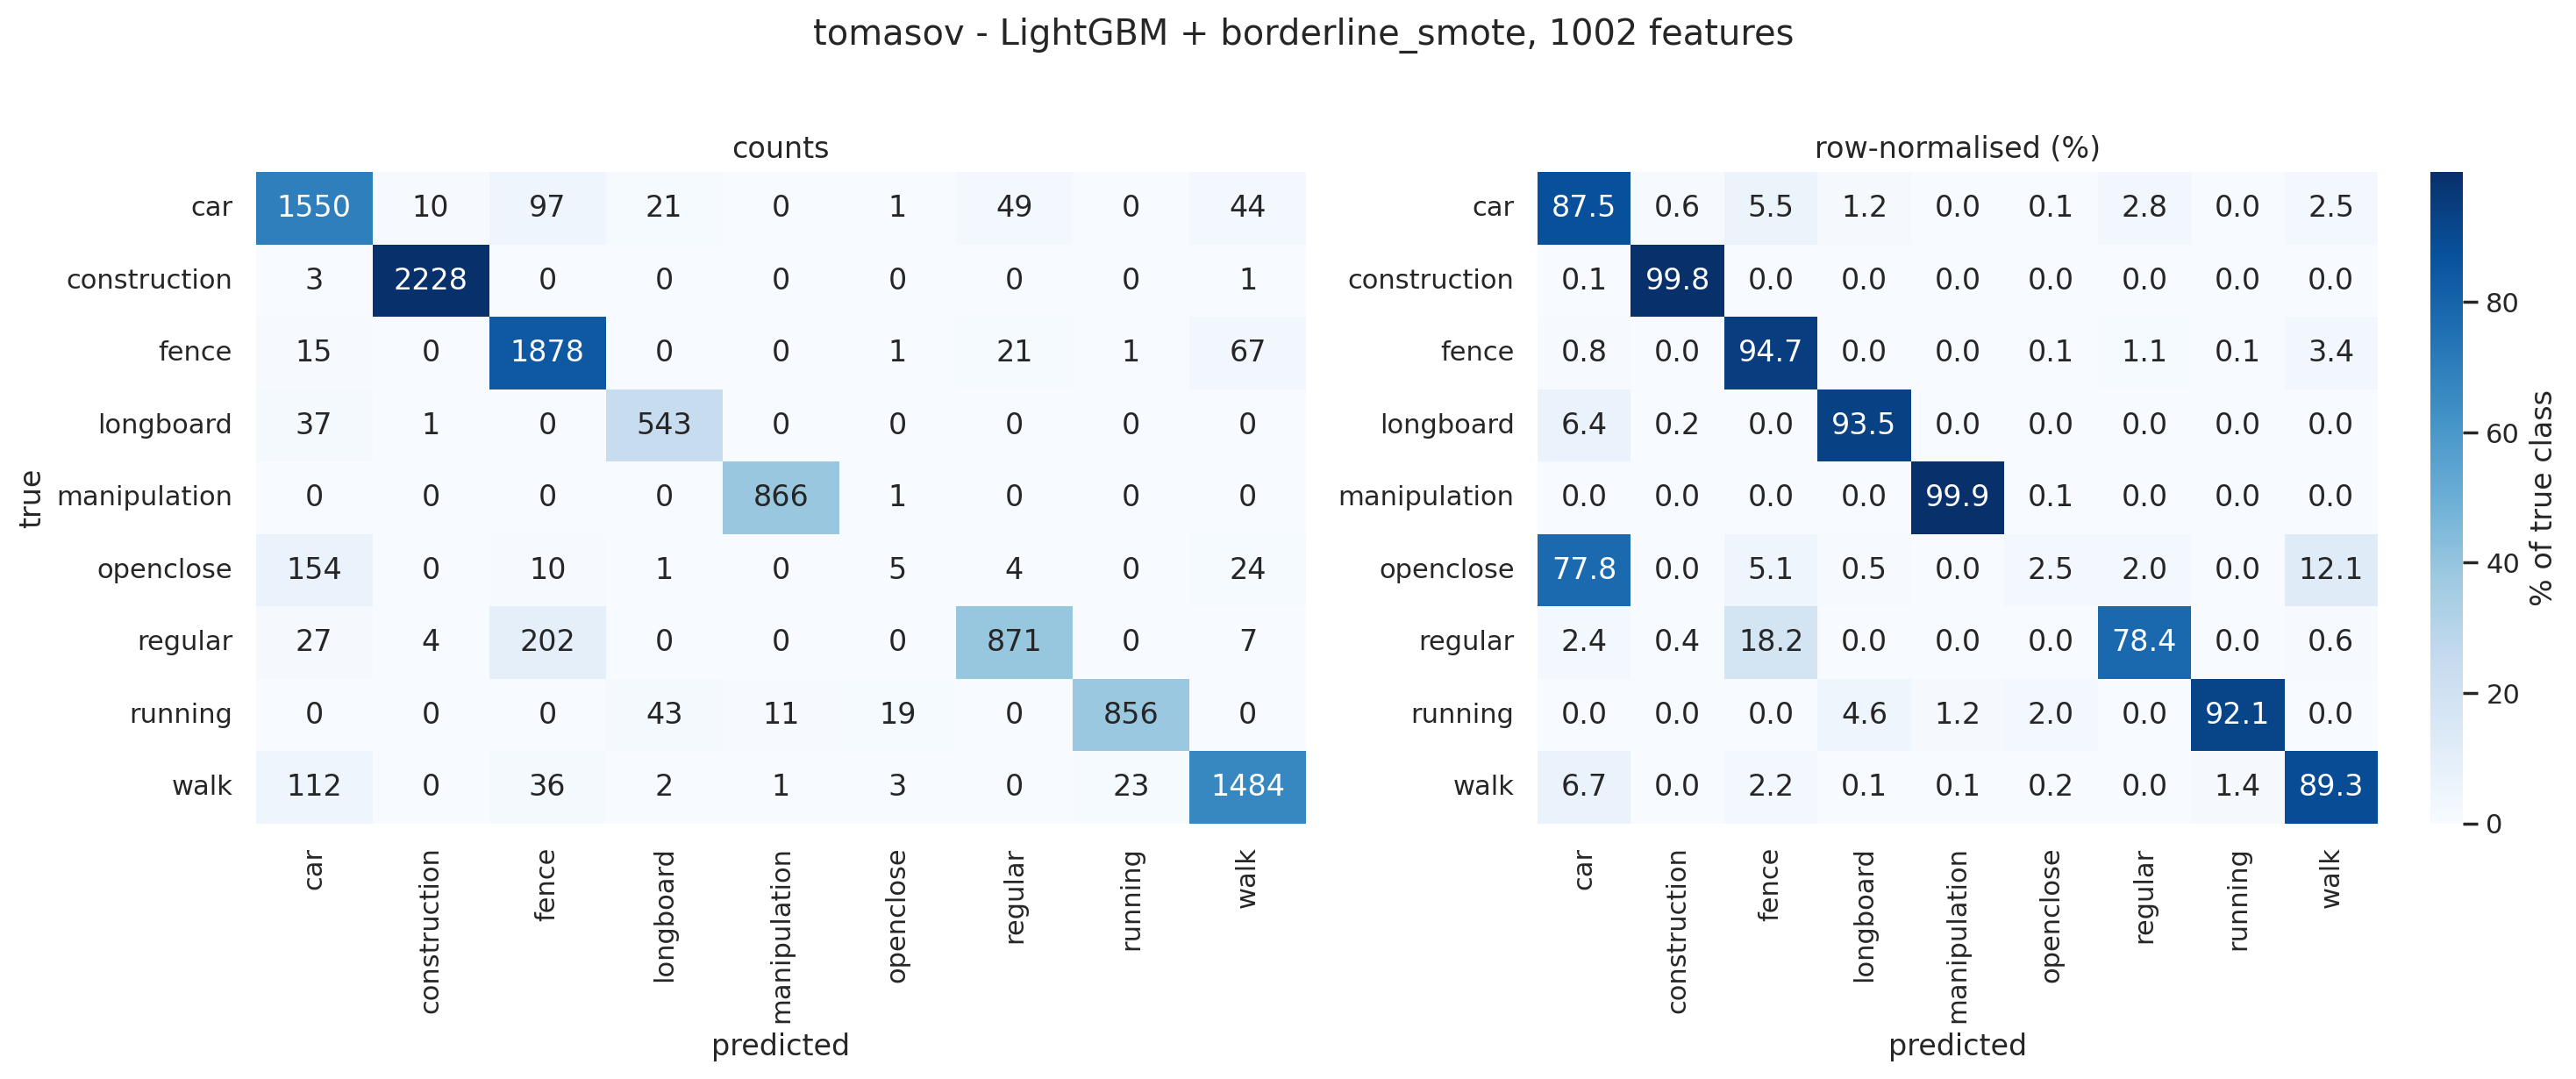
\includegraphics[width=0.9\textwidth,keepaspectratio]{Figures/fig19_confusion_tomasov.png}
\caption{Row-normalised confusion matrix of the selected LightGBM configuration, Tomasov 2025, multi-domain feature set.}
\label{fig:confusion_tomasov}
\end{figure}

\begin{figure}[!htbp]
\centering
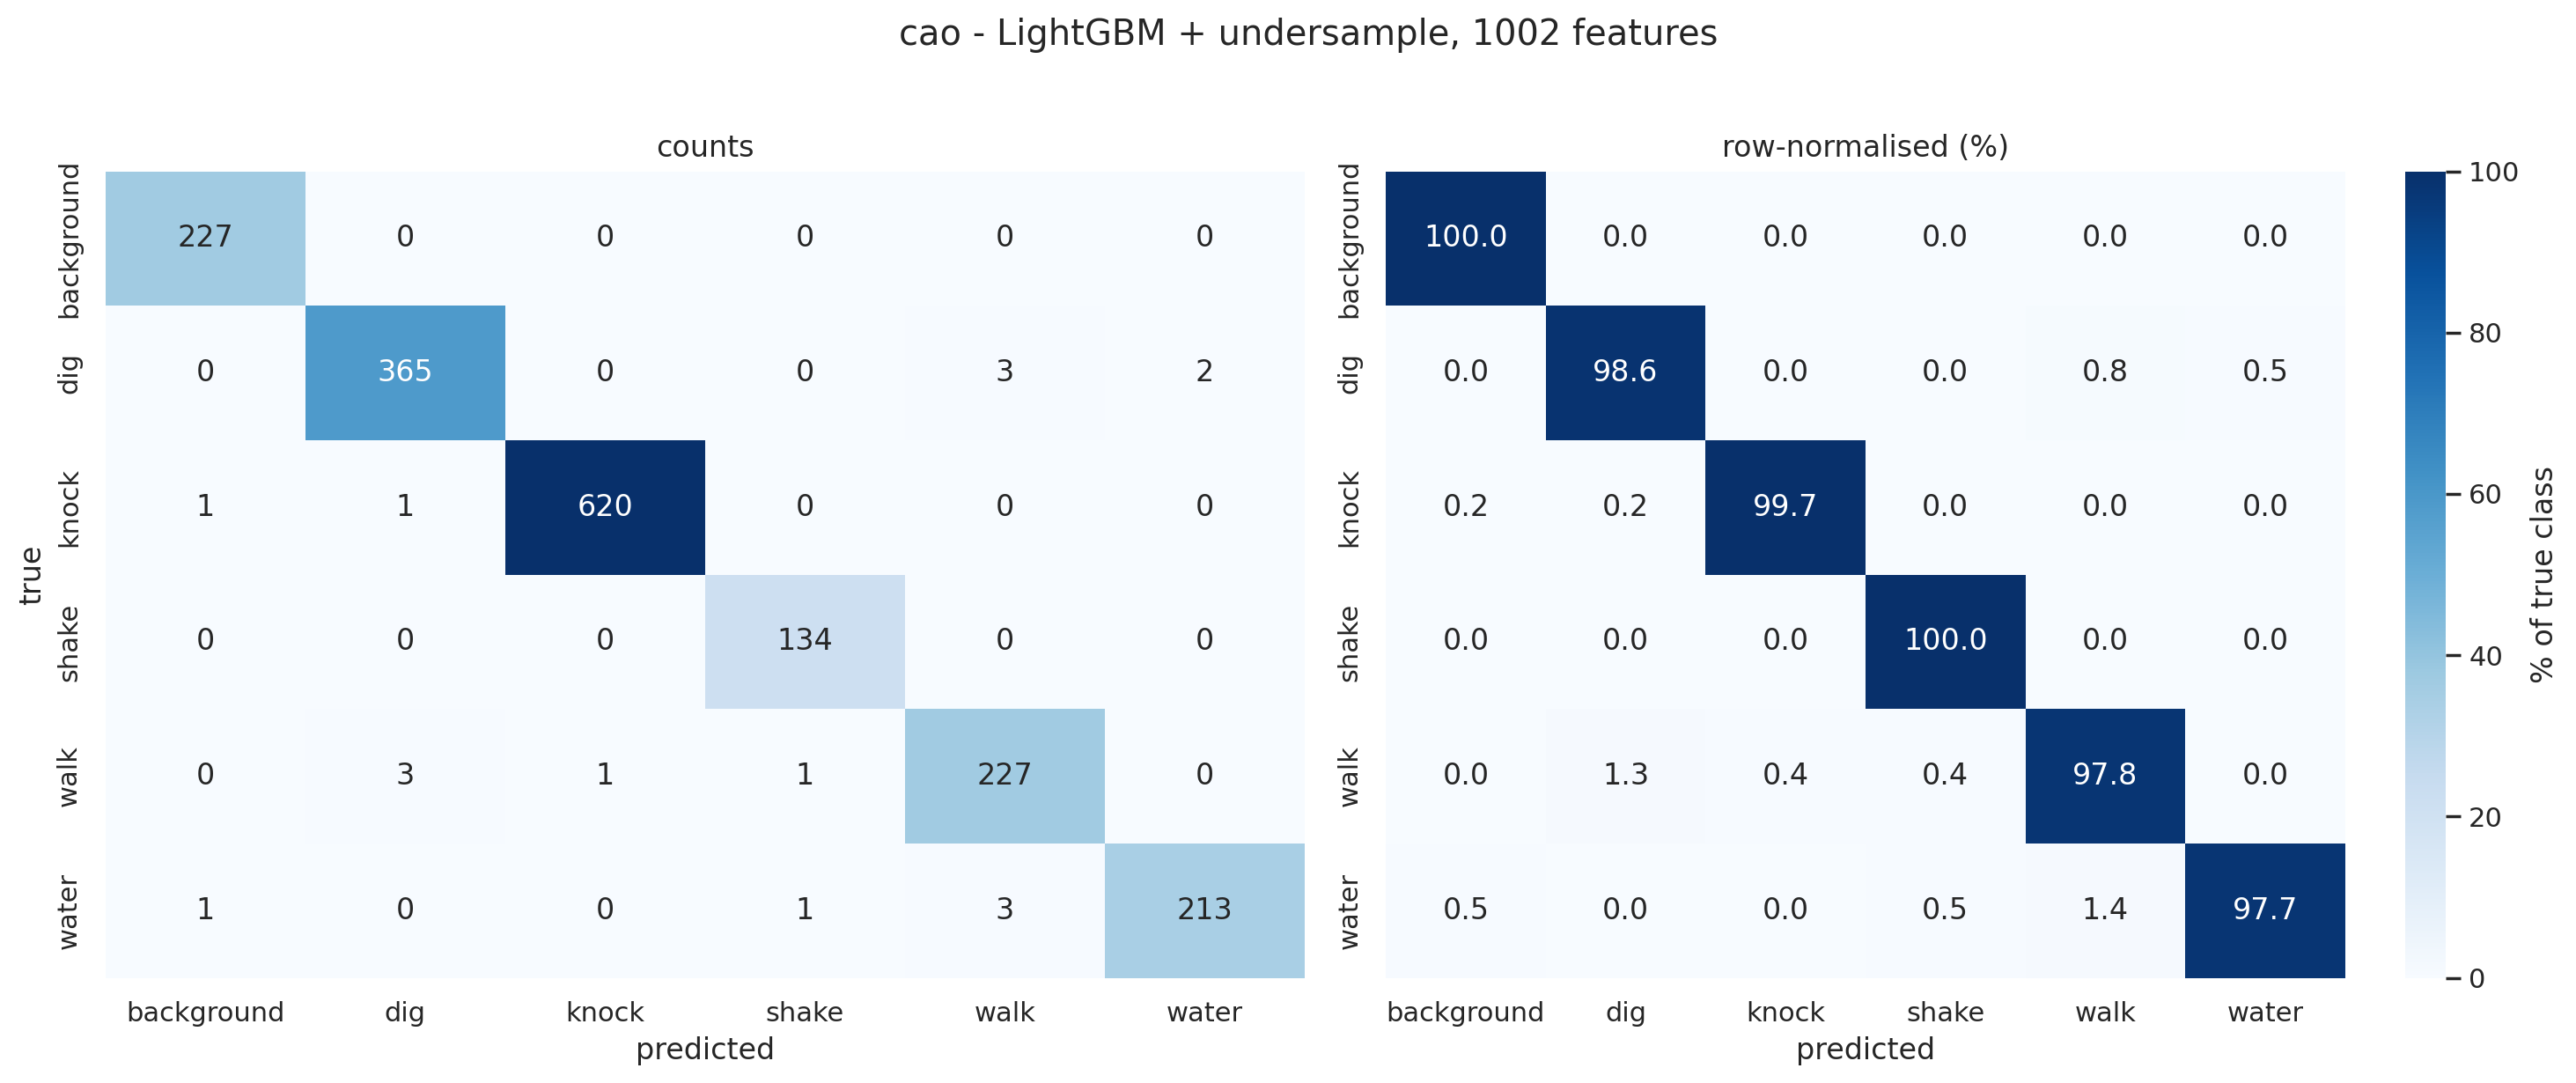
\includegraphics[width=0.9\textwidth,keepaspectratio]{Figures/fig20_confusion_cao.png}
\caption{Row-normalised confusion matrix of the selected LightGBM configuration, Cao 2023, multi-domain feature set.}
\label{fig:confusion_cao}
\end{figure}

\subsection{Performance on the \emph{Openclose} Class}
\label{sec:resOpenclose}
\autoBookmark{subsec}{Performance on the Openclose Class}
The most consequential single result is that none of the seven classifiers recognises \emph{openclose} (Table~\ref{tab:error_modes}). Its $F_1$ ranges from $0.000$ for random forest to $0.189$ for logistic regression; for the selected LightGBM it is $0.044$ with $2.5\%$ recall, with $77.8\%$ of its test windows classified as \emph{car} and a further $12.1\%$ as \emph{walk}. Every learner assigns the largest share of the class to \emph{car}, between $42.9\%$ (extremely randomised trees) and $91.4\%$ (random forest) of its windows, and all seven assign the next largest share to \emph{walk}. Under the previously published protocol the same class attained an $F_1$ of $0.72$ with $70\%$ recall.

\begin{table}[!htbp]
	\centering
	\caption{The two dominant Tomasov error modes across all seven classifiers. P, R, and $F_1$ refer to \emph{openclose}; the arrows give the percentage of a true class's test windows assigned to the named class; the last column is the recall of \emph{regular}.}
	\label{tab:error_modes}
	\footnotesize
	\setlength{\tabcolsep}{4pt}
	\begin{tabular}{@{}lrrrrrrr@{}}
		\toprule
		& \multicolumn{5}{c}{\textbf{\emph{Openclose}} ($n = 198$)} & \multicolumn{2}{c}{\textbf{\emph{Regular}} ($n = 1{,}111$)}\\
		\cmidrule(lr){2-6}\cmidrule(lr){7-8}
		\textbf{Classifier} & \textbf{P} & \textbf{R} & \textbf{$F_1$} & \textbf{$\rightarrow$ car (\%)} & \textbf{$\rightarrow$ walk (\%)} & \textbf{$\rightarrow$ fence (\%)} & \textbf{R}\\
		\midrule
		LightGBM             & 0.167 & 0.025 & 0.044 & 77.8 & 12.1 & 18.2 & 0.784\\
		XGBoost              & 0.077 & 0.010 & 0.018 & 83.3 & 9.1 & 16.9 & 0.793\\
		HistGradientBoosting & 0.205 & 0.045 & 0.074 & 76.3 & 9.1 & 18.4 & 0.779\\
		LogisticRegression   & 0.379 & 0.126 & 0.189 & 54.0 & 21.7 & 32.7 & 0.650\\
		RandomForest         & 0.000 & 0.000 & 0.000 & 91.4 & 5.1 & 21.9 & 0.767\\
		ExtraTrees           & 0.043 & 0.030 & 0.035 & 42.9 & 30.8 & 12.7 & 0.857\\
		DecisionTree         & 0.032 & 0.061 & 0.042 & 79.8 & 8.6 & 19.3 & 0.732\\
		\bottomrule
	\end{tabular}
\end{table}

The earlier result was made possible by contamination. \emph{Openclose} is the smallest class ($6{,}792$ windows, $1.54\%$ of the annotated set) and originates from a single recording. A random split places neighbouring windows from that recording in the training set and allows the model to exploit their similarity. Removing the overlap eliminates this shortcut, and without it none of the seven learners recovers the class from the $1{,}002$-feature representation.

The failure lies in the representation rather than in the data or in any single learner. It is common to a linear model, a single tree, bagged ensembles, and three boosting implementations, so the choice of classifier cannot be its cause. On the identical blocked partition and the same 198 test windows, all three graph baselines exceed every feature-based classifier (\refss{sec:resSOTA}): the reimplemented S2-DyGNN achieves an \emph{openclose} $F_1$ of $0.625$ with $0.88$ precision and $0.48$ recall, above the $0.557$ that it reports under its own protocol, GCN reaches $0.433$, and GAT $0.278$. These values are derived from single training runs on a small class and should therefore not be interpreted too precisely (\refss{sec:chap5LimMethod}), but the pattern is consistent: the class carries usable signal that 61 aggregate spatial scalars cannot express. The detection of unauthorised manhole entry on this dataset requires a model that operates on the channel axis directly rather than on descriptors pooled across it, and the class is retained in the evaluation so that the reported metrics reflect that fact.

The directional sensitivity of the fibre may contribute to the residual difficulty. A straight fibre is most sensitive to strain along its axis, and broadside disturbances induce comparatively little axial strain~\cite{he2021review,zhan2020das}. Events that act predominantly perpendicular to the local fibre segment, as the lifting of a manhole cover beside the cable may, produce weaker signatures with a lower signal-to-noise ratio that overlap with those of other classes. This is consistent with the low recall observed, and it would cause missed detections under any representation.

\subsection{Confusion Between Regular and Fence Events}
\label{sec:resErrors}
\autoBookmark{subsec}{Confusion Between Regular and Fence Events}
The second dominant confusion is that of \emph{regular} with \emph{fence}, which likewise occurs for every learner, affecting between $12.7\%$ (extremely randomised trees) and $32.7\%$ (logistic regression) of the \emph{regular} windows (Table~\ref{tab:error_modes}). For the selected LightGBM the proportion is $18.2\%$, which is consistent with overlapping low-amplitude vibration patterns and with the $12.2\%$ reported previously. Errors in this direction raise false fence-intrusion alerts and increase operator workload in the absence of a genuine security event, which makes this the error mode most relevant to nuisance-alarm budgeting. Extremely randomised trees also exhibit the reverse tendency, assigning $42.8\%$ of the \emph{fence} windows to \emph{regular}, which would instead suppress genuine intrusion alerts; the boosted learners limit that reverse confusion to about $1\%$. \emph{Car}, \emph{fence}, and \emph{regular} therefore form a confusable cluster, and the treatment of this cluster distinguishes the strong learners from the weak ones on this dataset more than any other factor.

\section{Statistical Testing}
\label{sec:resStats}
\autoBookmark{sec}{Statistical Testing}
Statistical testing follows the performance evaluation in \reff{fig:methodology_framework}, because a difference between configurations is meaningful only when it exceeds the variation expected from the data themselves. An earlier version of this analysis applied the Friedman test with the six balancing strategies as blocks and the seven classifiers as treatments, and obtained $\chi^2_F = 35.43$ against an attainable maximum of $36$. As \refss{sec:chap3Statistics} explains, those blocks are not independent replicates, and the near-maximal statistic reflects their dependence rather than a strong effect. That analysis was therefore withdrawn and replaced by the three tests reported below, whose units of replication are independent.

\paragraph[Partition Variance]{Partition Variance.}
Repeating the leakage-controlled partition with five seeds over the same population yields a macro-$F_1$ of $80.47 \pm 4.42$ on Tomasov (range $74.52$--$84.99$) and $99.13 \pm 0.30$ on Cao for the selected LightGBM configuration (\reff{fig:repeated_splits}). The single-partition headline values of $81.98$ and $98.90$ lie within those ranges, but the Tomasov range of $10.5$ points implies that every headline figure on that dataset must be accompanied by its partition standard deviation. The ranking of the classifiers is stable across all five partitions on both datasets even though the absolute level is not: LightGBM leads random forest and logistic regression on every seed.

\begin{figure}[!htbp]
\centering
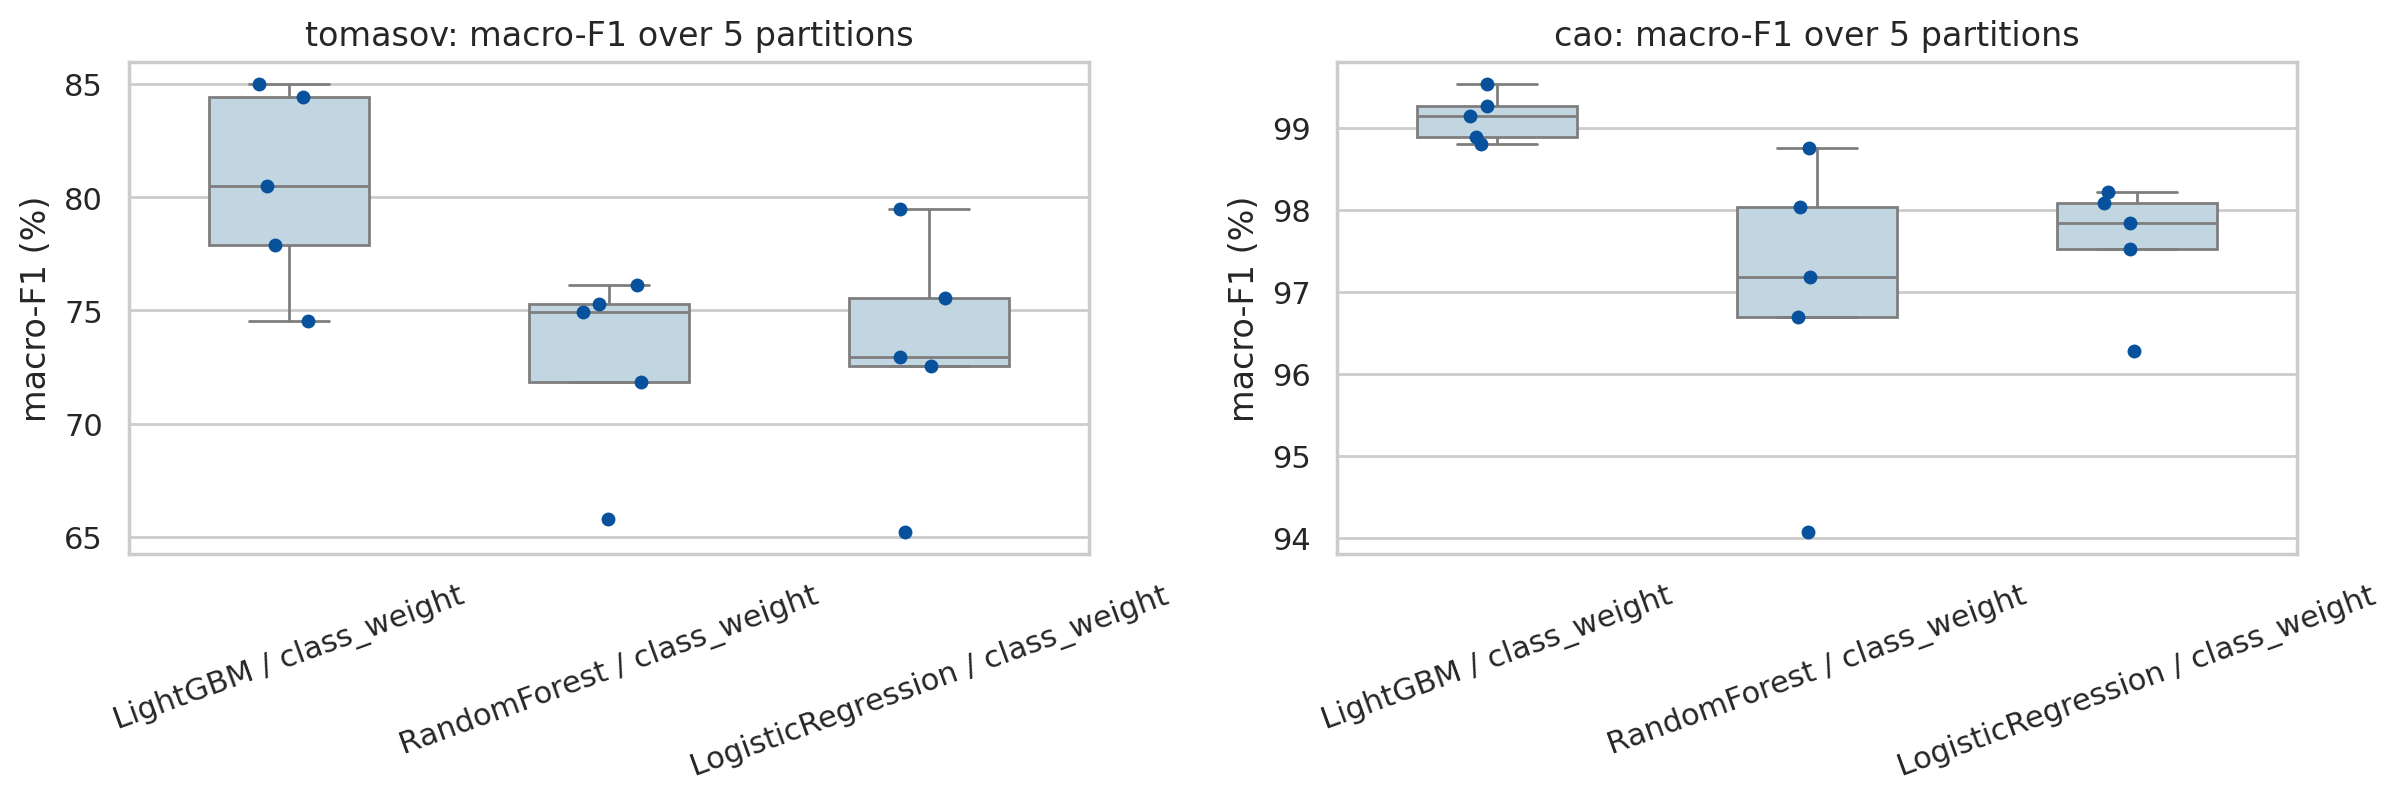
\includegraphics[width=0.95\textwidth,keepaspectratio]{Figures/fig36_repeated_splits.png}
\caption{Test macro-$F_1$ over five independently generated leakage-controlled partitions for three classifiers with class weighting: Tomasov (left) and Cao (right).}
\label{fig:repeated_splits}
\end{figure}

\paragraph[Group Bootstrap Intervals]{Group Bootstrap Intervals.}
Bootstrapping the reported test set over whole acquisitions rather than individual windows widens the $95\%$ interval by an order of magnitude on Tomasov: the interval on accuracy increases from $\pm 0.53$ at window level to $\pm 5.89$ by zone and $\pm 7.58$ by recording (\reff{fig:bootstrap_ci}). On Cao the interval changes only marginally ($\pm 0.42$ to $\pm 0.52$ by date), which indicates that the Cao acquisitions are homogeneous in accuracy whereas the Tomasov recordings are not. Window-level intervals treat overlapping windows as independent observations; as a result, they understate the uncertainty and are quoted only for comparison. Macro-$F_1$ is not estimable at the coarser levels on Tomasov, because a resample of thirteen recordings routinely omits entire classes; accuracy is therefore reported at recording level and macro-$F_1$ at zone level.

\begin{figure}[!htbp]
\centering
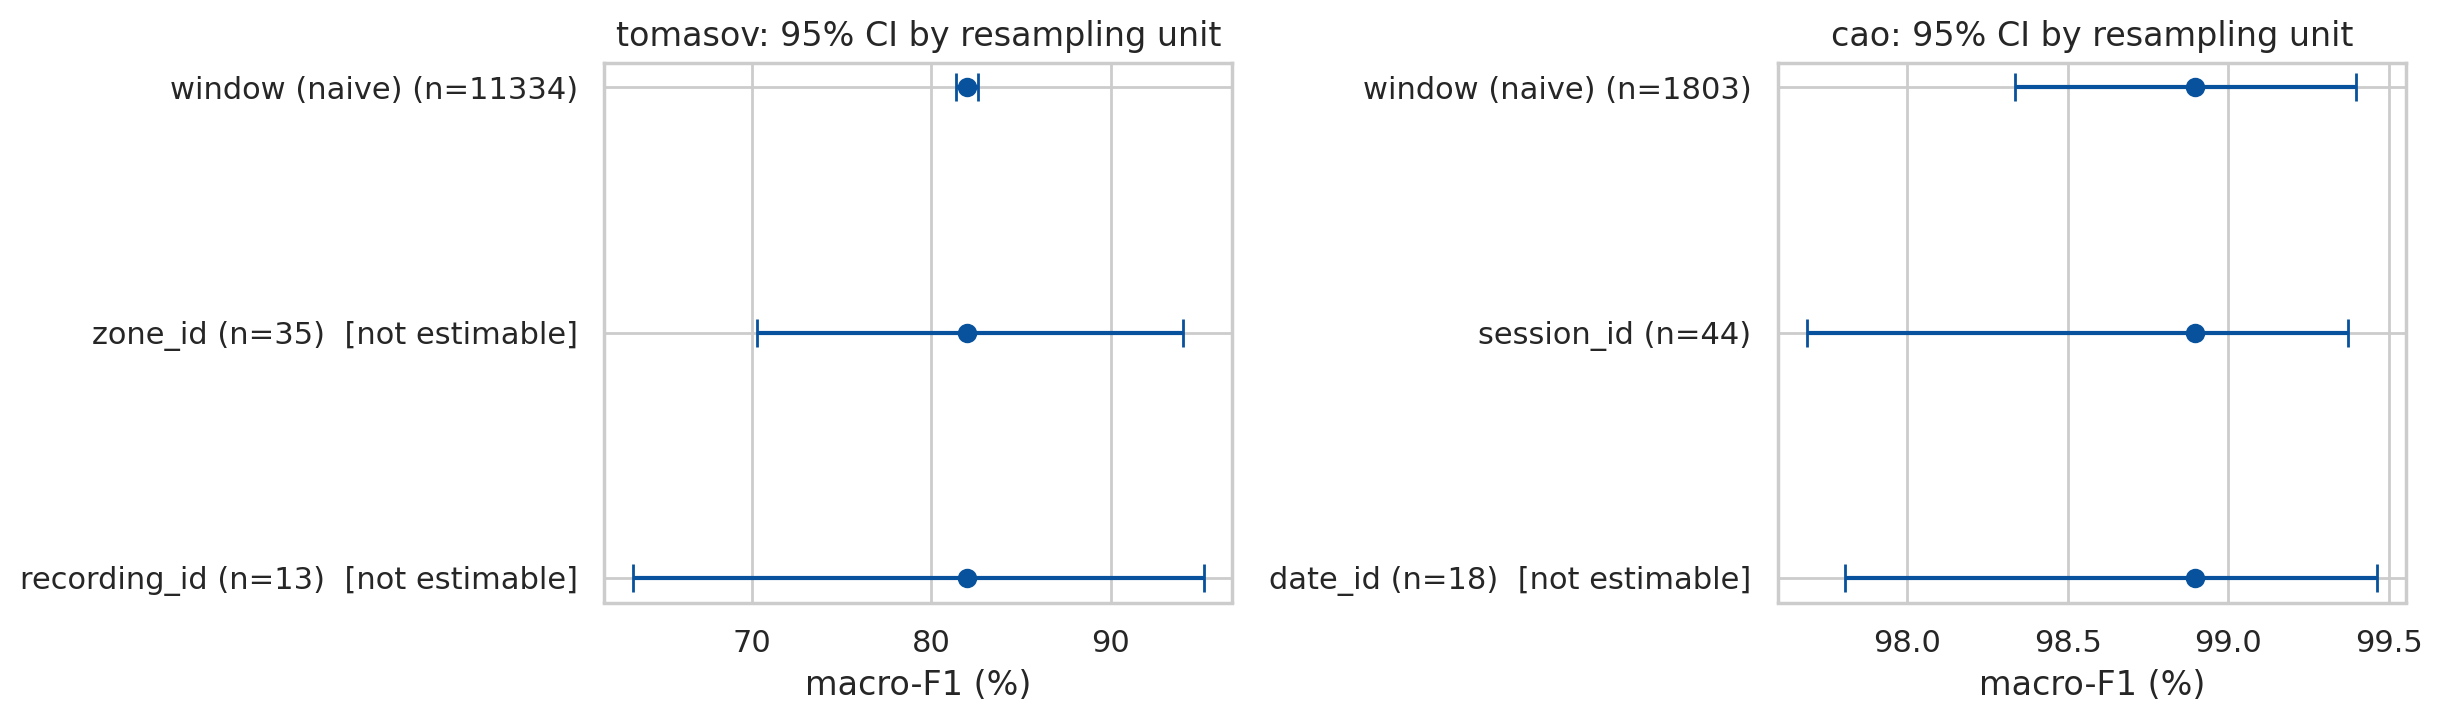
\includegraphics[width=0.95\textwidth,keepaspectratio]{Figures/fig37_group_bootstrap_ci.png}
\caption{$95\%$ bootstrap confidence intervals on test macro-$F_1$ by resampling unit: Tomasov (left) and Cao (right). Intervals marked not estimable are those in which resamples routinely omit entire classes.}
\label{fig:bootstrap_ci}
\end{figure}

\paragraph[Paired Comparison over Independent Acquisitions]{Paired Comparison over Independent Acquisitions.}
The six balancing strategies were compared again with each block consisting of a whole held-out acquisition, the model being trained on all the others, and with Holm correction across the family of pairwise comparisons~\cite{holm1979simple,demsar2006statistical}. On Tomasov, eleven held-out recordings distinguish two pairs: undersampling exceeds class weighting by $5.13$ points (corrected $p = 0.041$), and Borderline-SMOTE exceeds it by $1.44$ points (corrected $p = 0.029$). On Cao, ten held-out dates distinguish no pair of strategies on either metric (smallest corrected $p = 0.82$; the six strategies span $0.45$ accuracy points). The choice of strategy therefore has a modest effect on Tomasov and no detectable effect on Cao, in contrast to the uniform significance that the Friedman test had reported.

\section{Spatial-Domain Confound Analysis}
\label{sec:resConfound}
\autoBookmark{sec}{Spatial-Domain Confound Analysis}
High scores do not in themselves reveal what a model has learnt, and this section examines whether the measured performance reflects the events or the recordings in which they were captured. \refs{sec:resDomains} showed that 61 spatial features outperform 739 time--frequency features on Tomasov, which reverses the ordering reported in earlier single-dataset work. Spatial descriptors summarise fibre geometry, coupling, and the channel-to-channel energy structure, all of which are largely fixed within a recording, and five of the nine Tomasov classes each originate from a single recording. Part of the observed performance may therefore be attributable to recording identification rather than to event discrimination. The diagnostics of \refss{sec:chap3ConfoundDesign} test this possibility directly.

\subsection{Leave-One-Domain-Out Ablation}
\label{sec:resLODO}
\autoBookmark{subsec}{Leave-One-Domain-Out Ablation}
With the model and balancing strategy fixed at LightGBM with class weighting, so that only the feature set varies, removing the spatial block reduces macro-$F_1$ by $19.67$ points on Tomasov ($81.81$ to $62.13$) and by $5.14$ on Cao ($98.89$ to $93.75$). Removing any other domain reduces the Tomasov score by less than $0.3$ points (\reff{fig:domain_removal}). The spatial features therefore carry information that the other three domains cannot replace, whereas each of the other domains is largely redundant given the remainder. This asymmetry is the reason why the spatial domain warrants scrutiny: if its contribution were recording identity rather than event information, the Tomasov headline figure would overstate the performance that a deployment could achieve.

\begin{figure}[!htbp]
\centering
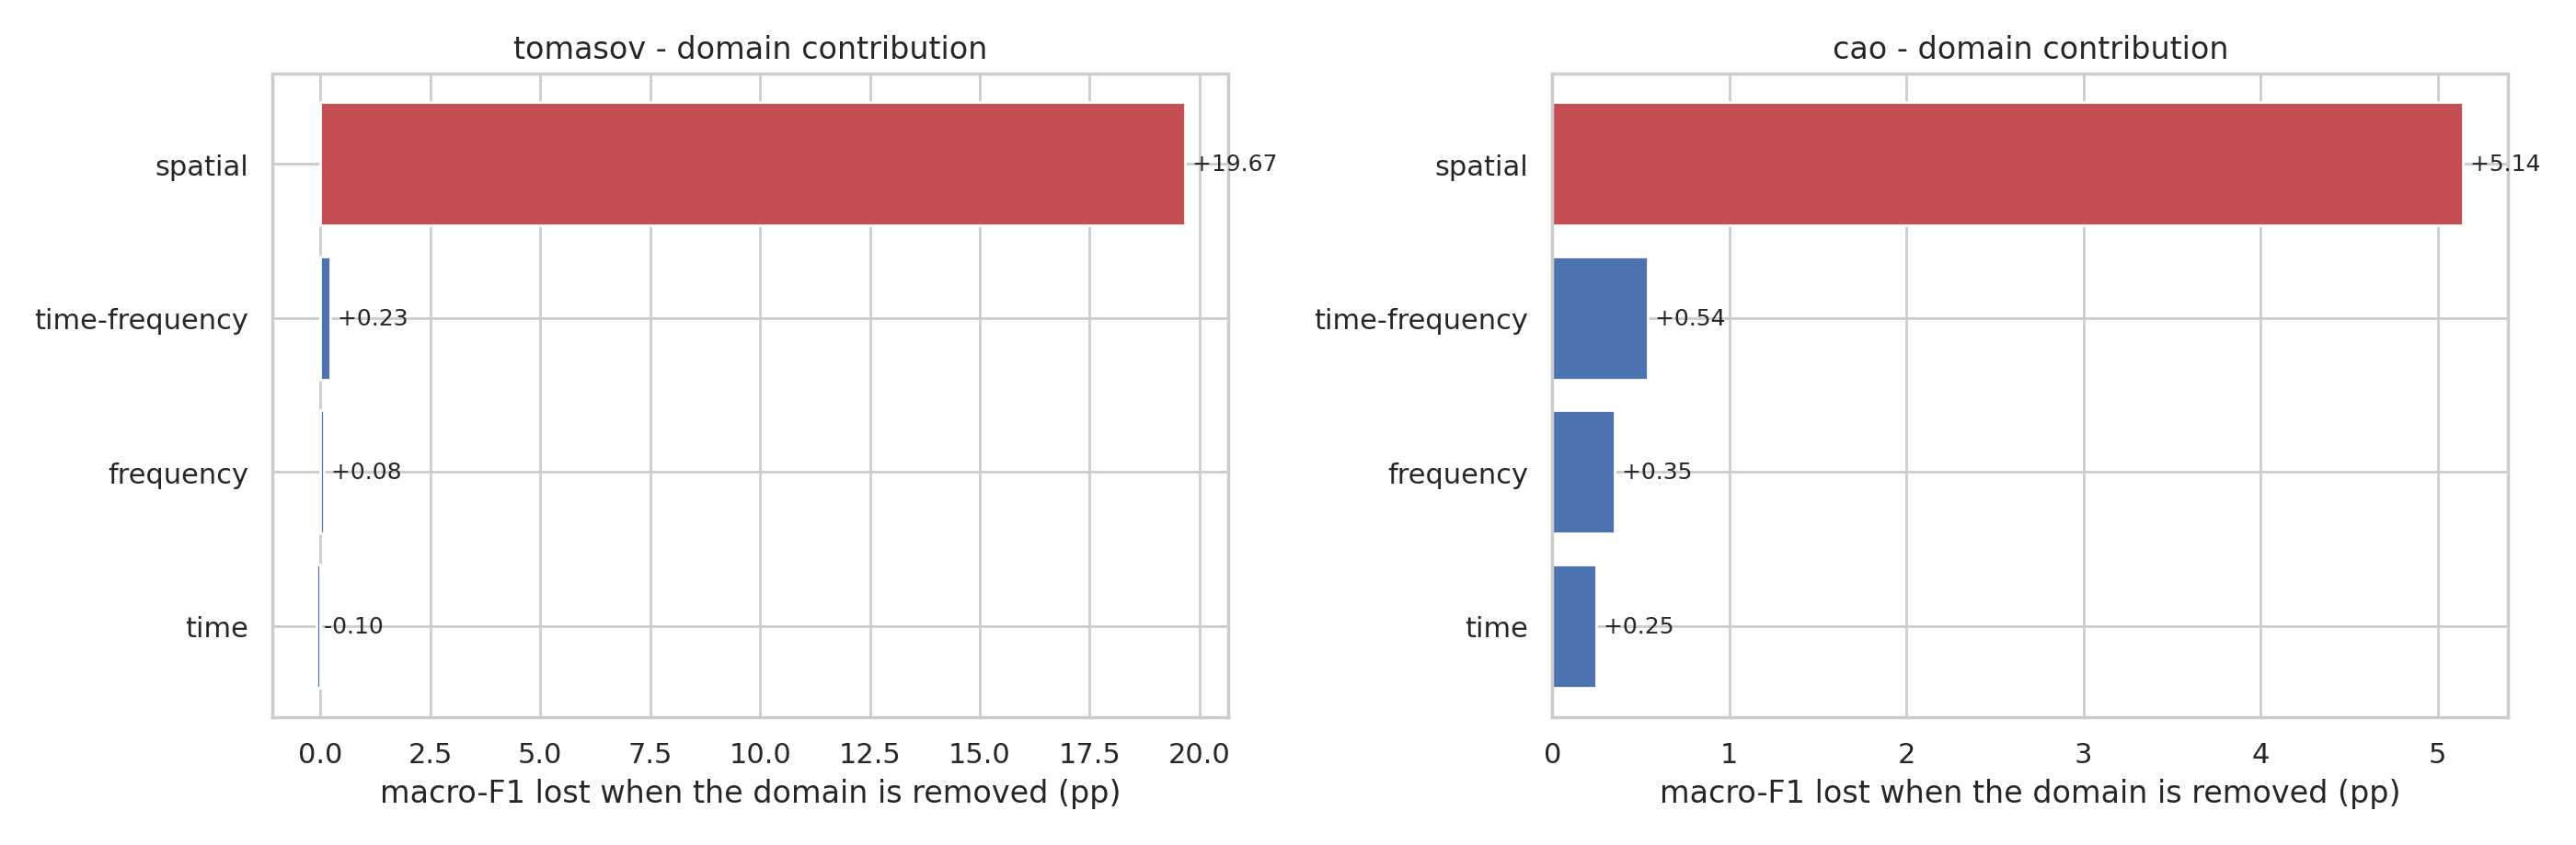
\includegraphics[width=0.9\textwidth,keepaspectratio]{Figures/fig21_domain_removal.png}
\caption{Macro-$F_1$ lost when each domain is removed from the fused representation.}
\label{fig:domain_removal}
\end{figure}

\subsection{Recording-Identity Probe}
\label{sec:resProbe}
\autoBookmark{subsec}{Recording-Identity Probe}
\reff{fig:recording_probe} presents the result of holding the event class fixed and using each domain to predict the source recording. On Tomasov, spatial features identify the recording $12.9$ points above chance, $11.1$ points more than the strongest alternative domain ($1.8$). On the \emph{car} class alone, spatial descriptors attain a recording-identification accuracy of $97.2\%$, whereas the time, frequency, and time--frequency domains remain within $0.4$ points of the majority baseline or fall below it. The spatial descriptors therefore act, at least in part, as a fingerprint of the recording in which an event was captured.

\begin{figure}[!htbp]
\centering
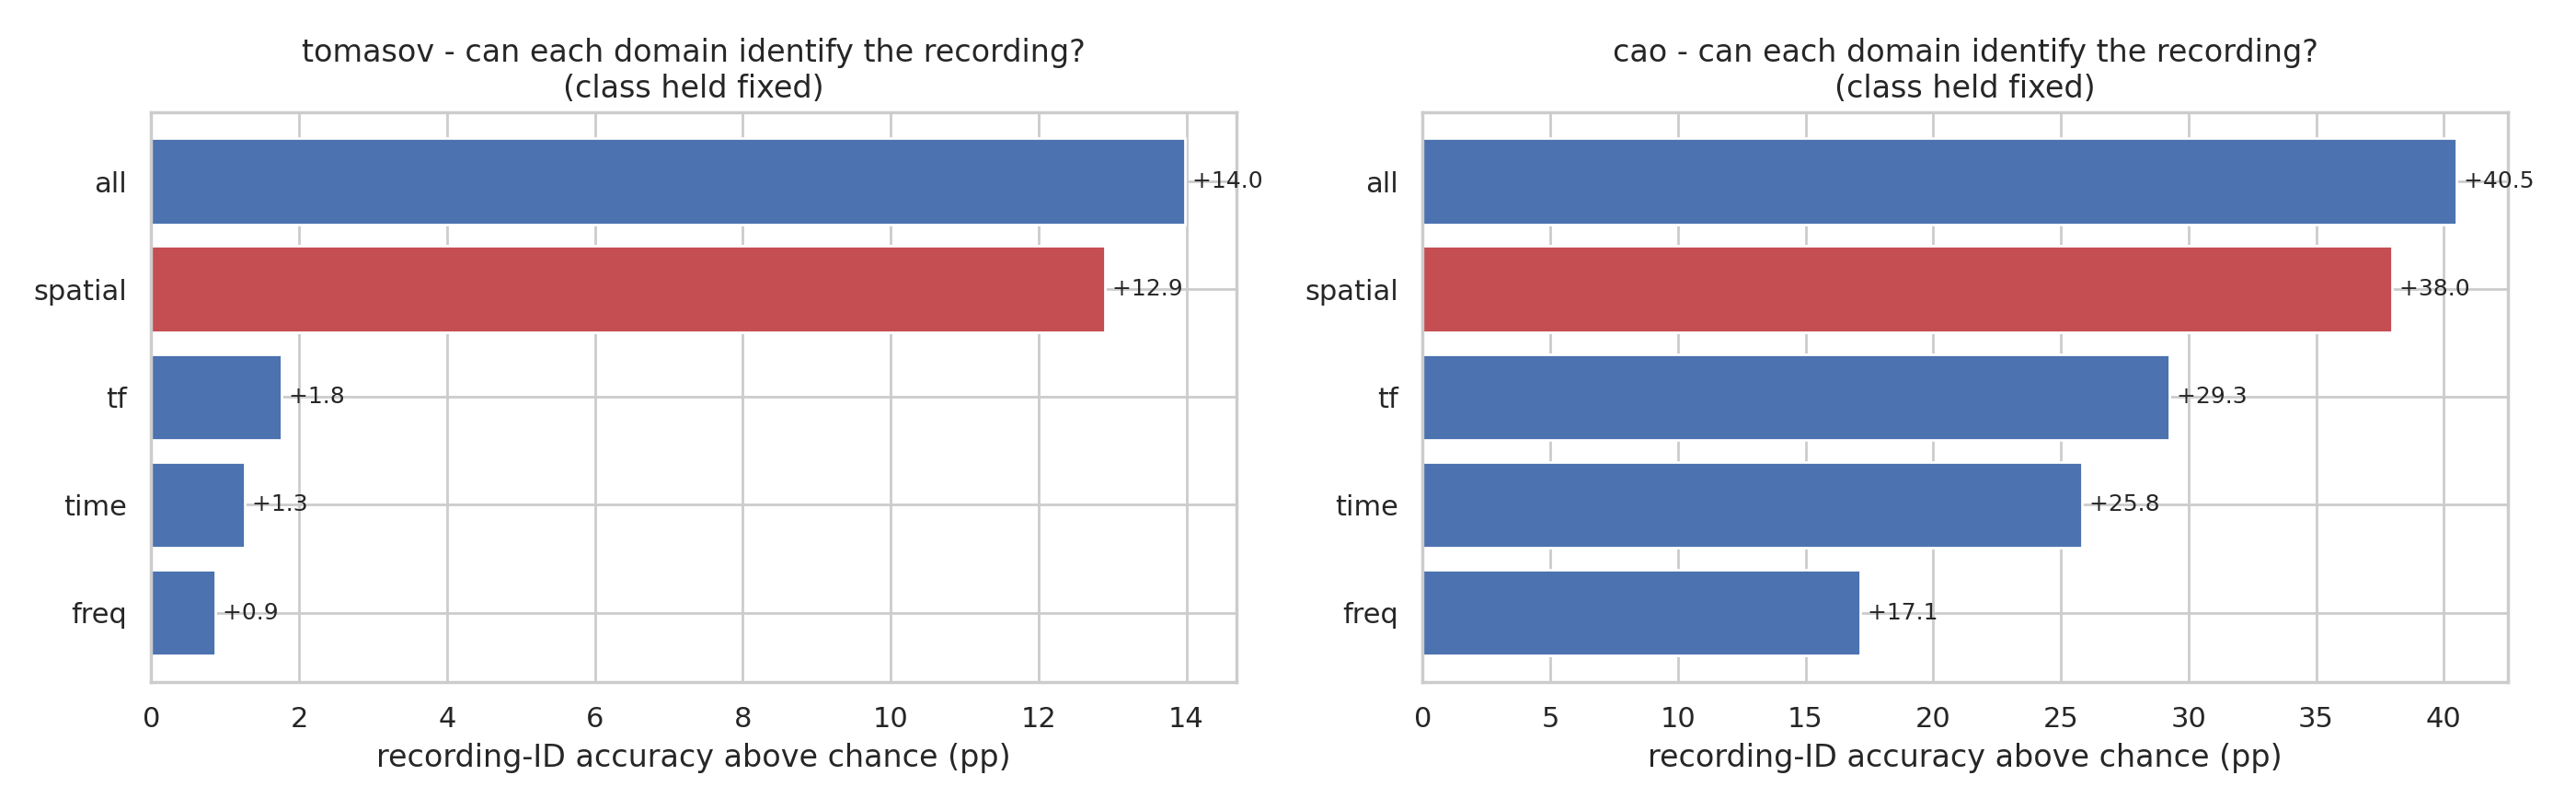
\includegraphics[width=0.9\textwidth,keepaspectratio]{Figures/fig22_recording_probe.png}
\caption{Recording-identification accuracy above chance, by feature domain, with the event class held fixed.}
\label{fig:recording_probe}
\end{figure}

\subsection{Leave-One-Recording-Out Evaluation}
\label{sec:resLORO}
\autoBookmark{subsec}{Leave-One-Recording-Out Evaluation}
The spatial features are not purely recording-specific, however. Under leave-one-recording-out evaluation, removing them reduces cross-recording accuracy by $19.08$ points on average, and only 4 of the 11 held-out recordings improve (\reff{fig:loro_spatial}). If the spatial block were purely a fingerprint, discarding it could not degrade generalisation to a recording whose fingerprint was never available during training. The motion and propagation descriptors plausibly capture physical characteristics of the events: a passing vehicle traces a spatial-centroid trajectory that remains informative across recordings.

\begin{figure}[!htbp]
\centering
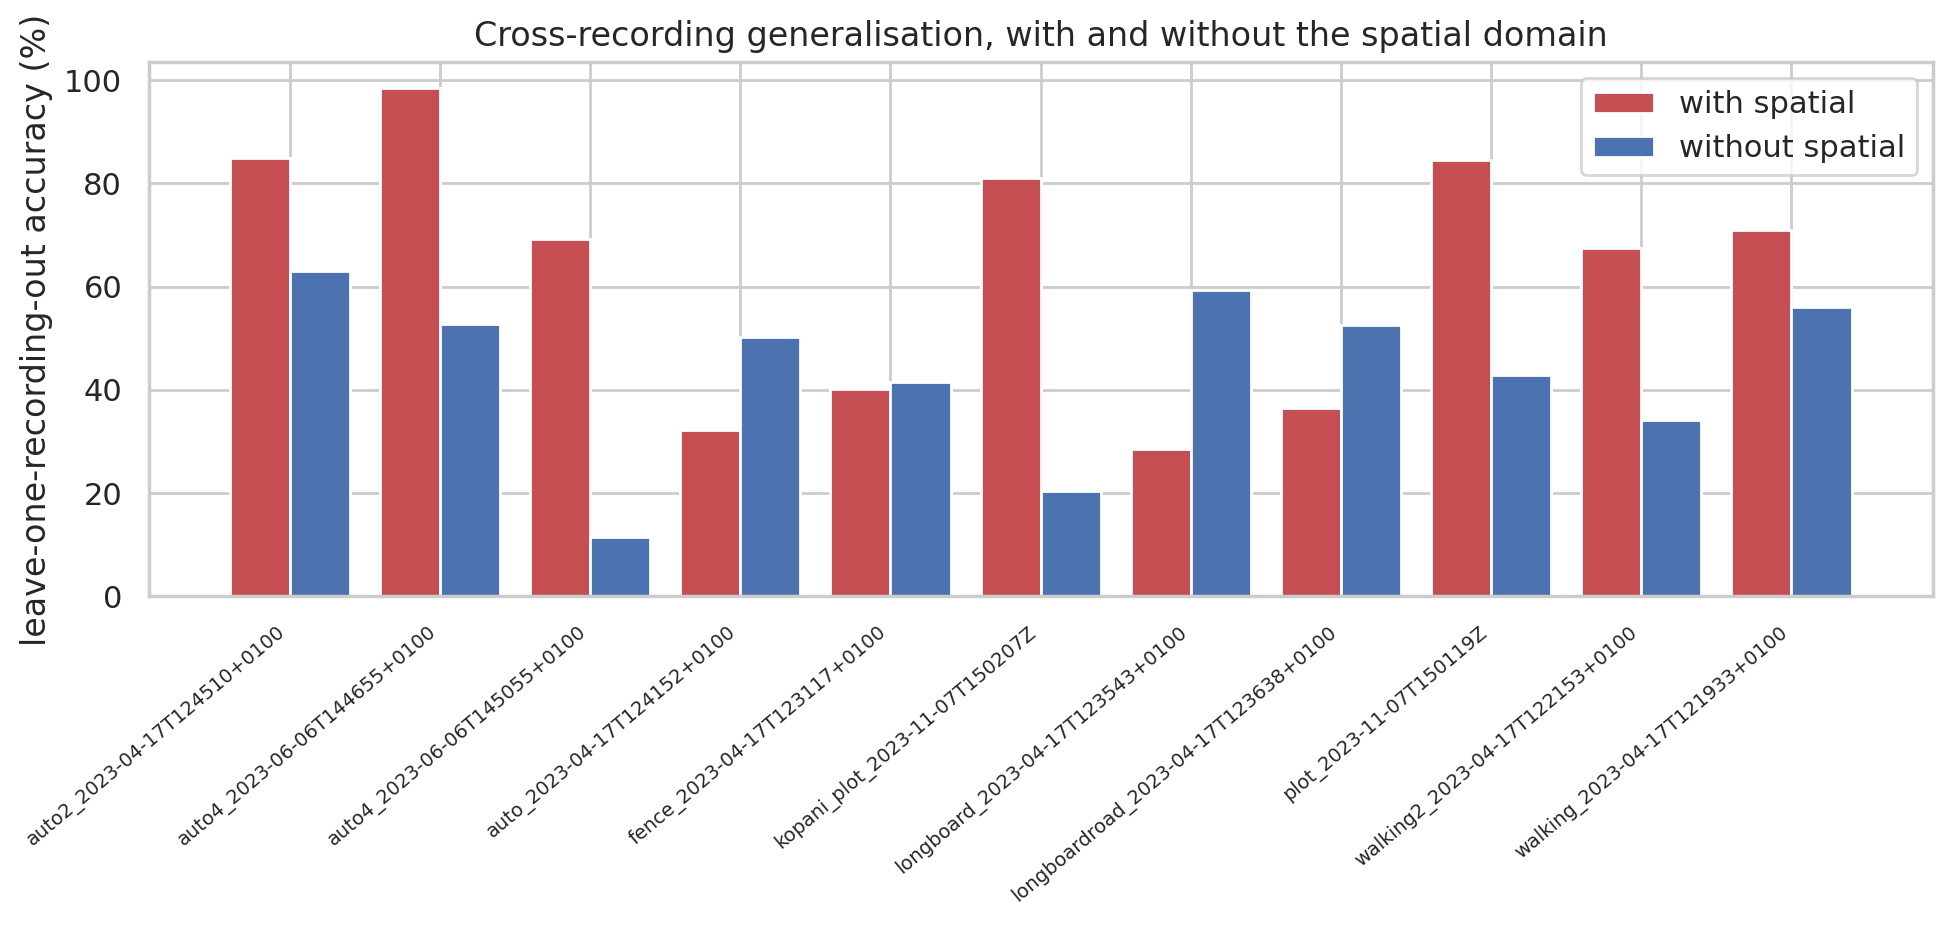
\includegraphics[width=0.9\textwidth,keepaspectratio]{Figures/fig23_loro_spatial.png}
\caption{Leave-one-recording-out accuracy with and without the spatial domain. The wide per-recording range of the difference ($-60.7$ to $+30.8$ points) indicates a mixture of transferable and recording-specific information.}
\label{fig:loro_spatial}
\end{figure}

\subsection{Implications for Reporting}
\label{sec:resConfoundVerdict}
\autoBookmark{subsec}{Implications for Reporting}
Spatial descriptors carry both transferable propagation information and recording-specific variation, and this dataset cannot separate the two, because for five of the nine classes the recording and the class are the same variable. Two figures are therefore reported for Tomasov. Where deployment recordings are represented in training, the selected configuration of Table~\ref{tab:main_results} reaches a macro-$F_1$ of $81.98$ with all features. Where they are not, a conservative figure of $62.13$ is reported, obtained by removing the spatial block. That figure is taken from the leave-one-domain-out ablation, whose all-feature reference under the same fixed configuration is $81.81$, so the cost attributable to the spatial descriptors is $19.67$ points rather than the $19.85$ that a comparison with Table~\ref{tab:main_results} would suggest.

The Cao dataset yields a different diagnosis. On this dataset the spatial margin is $8.7$ points, but every domain identifies the acquisition date well above chance ($38.0$ points for the spatial domain and $29.3$ for the strongest alternative). The confound is therefore not specific to the spatial domain but is a dataset-wide campaign confound: the entire feature space encodes acquisition conditions, which explains the decline in cross-campaign performance reported in \refs{sec:resGeneralisation}. The \emph{openclose} comparison of \refss{sec:resOpenclose} bounds the cost of aggregation over the channel axis, since a model that retains that axis recovers a class that the pooled descriptors cannot. Taken together, these findings show that the recording confound cannot be removed by partitioning alone, and they motivate the stricter generalisation tests that follow. \reff{fig:feature_importance} shows the importance distribution of the final Tomasov model by domain.

\begin{figure}[!htbp]
\centering
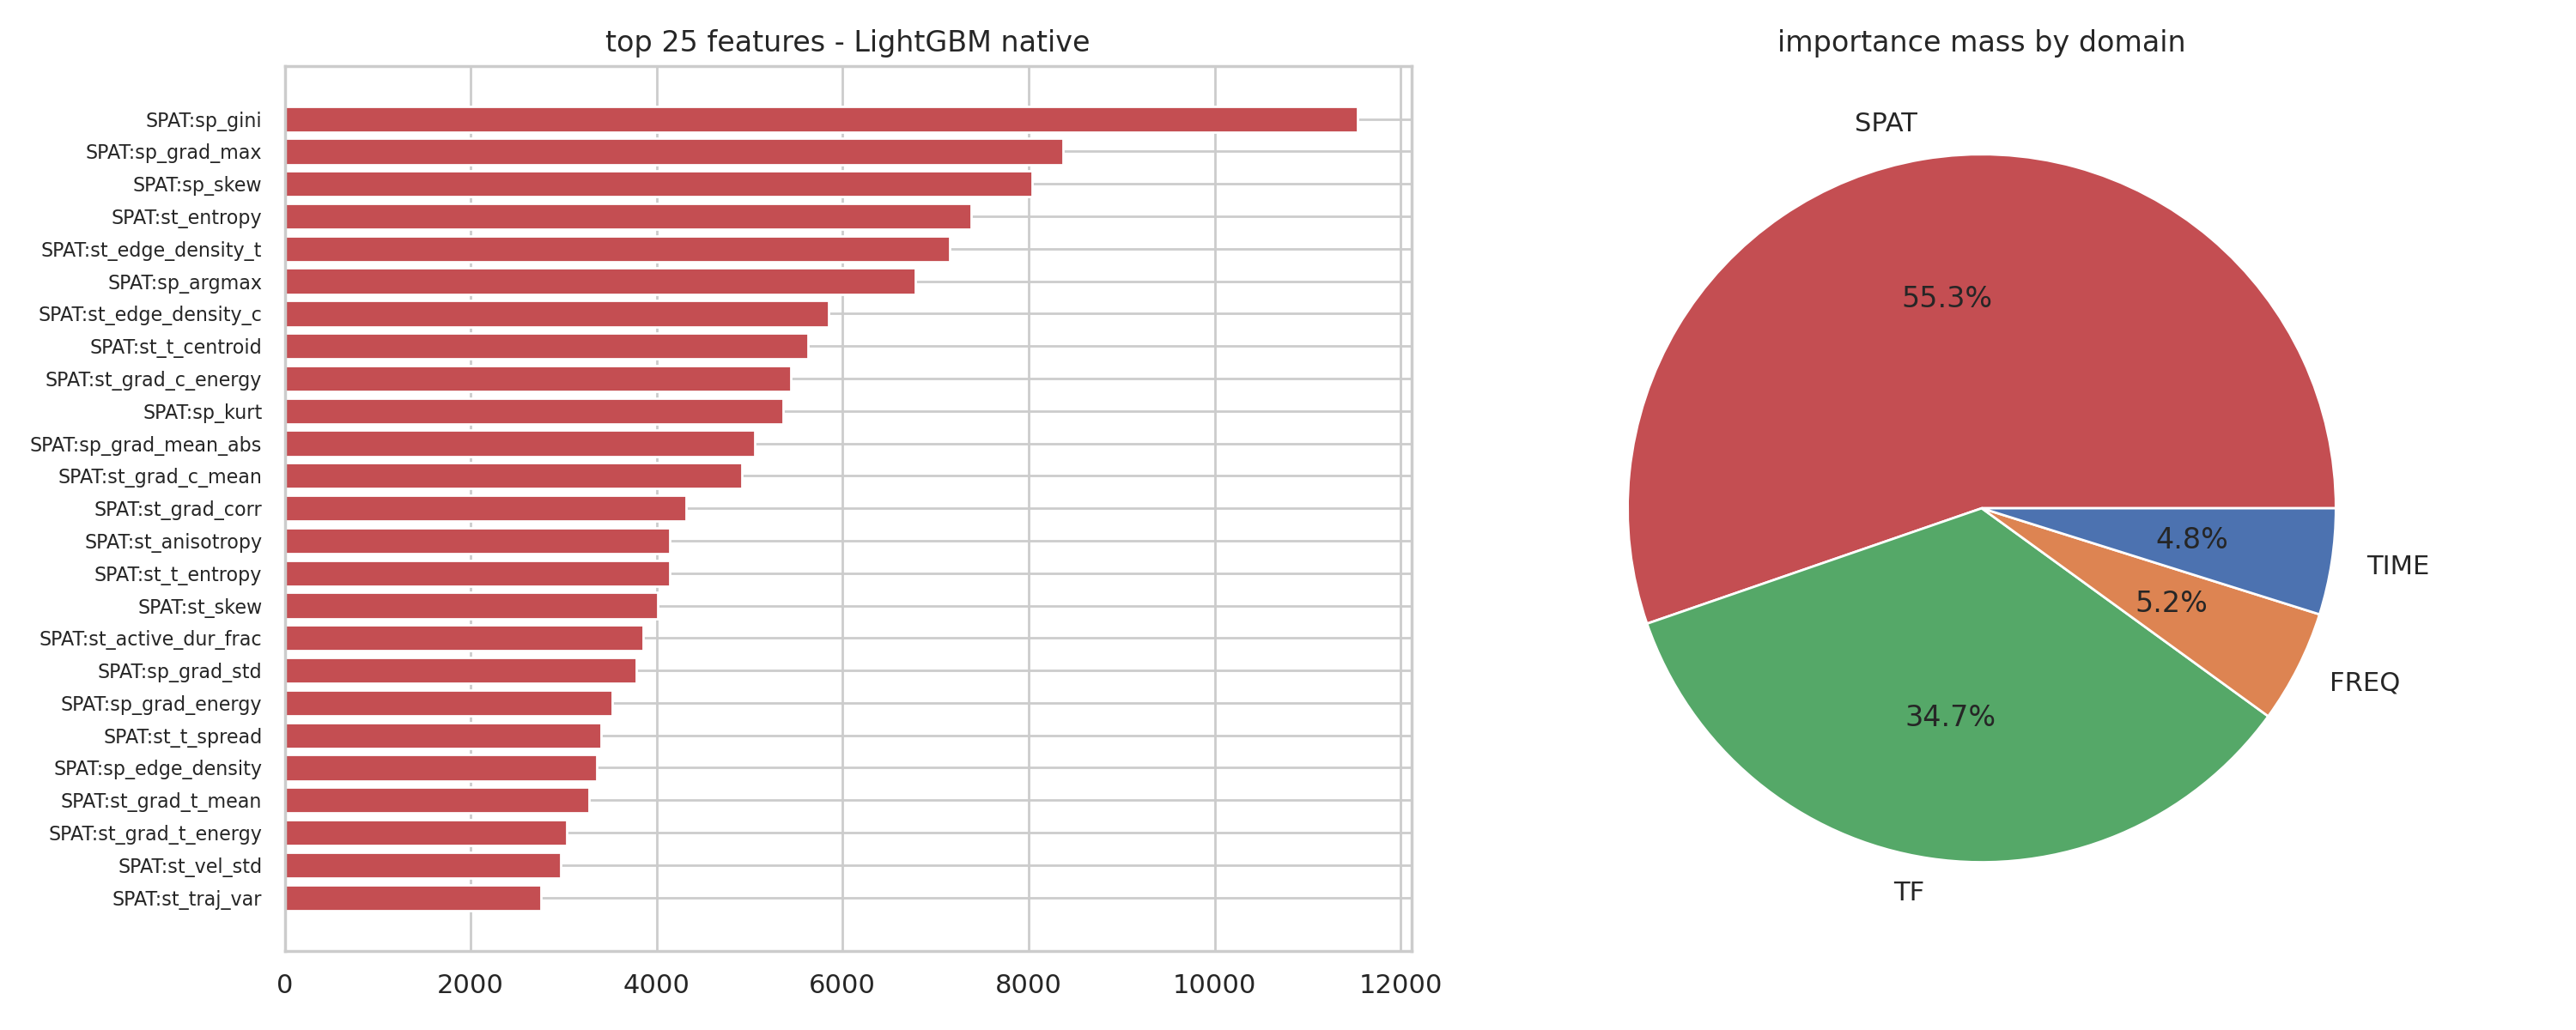
\includegraphics[width=0.95\textwidth,keepaspectratio]{Figures/fig26_feature_importance.png}
\caption{Feature importance for the final Tomasov model, coloured by domain.}
\label{fig:feature_importance}
\end{figure}

\section{Generalisation Evaluation}
\label{sec:resGeneralisationAll}
\autoBookmark{sec}{Generalisation Evaluation}
The partitions of \refs{sec:resLeakage} measure generalisation to unseen segments of recordings that are represented in training, which is a weaker requirement than generalisation to new acquisitions. This section and the next apply the stricter protocols of \refss{sec:chap3ConfoundDesign}. \refss{sec:resGeneralisation} holds out whole recordings and acquisition dates, and \refss{sec:resConsistency} examines whether the pipeline behaves consistently on the two systems. \refs{sec:resMapping} then maps the two event taxonomies onto each other and transfers a fitted model directly from one system to the other.

\subsection{Cross-Recording and Cross-Campaign Evaluation}
\label{sec:resGeneralisation}
\autoBookmark{subsec}{Cross-Recording and Cross-Campaign Evaluation}
On the four Tomasov classes recorded more than once, leave-one-recording-out accuracy averages $63.85\%$ (SD $29.31$), compared with $90.71\%$ within represented recordings, a reduction of $26.86$ points when generalising to an unseen recording. The per-recording range is wide, from $6.22\%$ to $99.05\%$ across the eleven held-out recordings, and the mean should therefore not be interpreted as a stable operating point.

On Cao, leave-one-date-out evaluation reduces accuracy from $99.06\%$ to $86.81\%$, with a range of $48.84\%$ to $100.00\%$ across the ten dates. The macro-$F_1$ figure requires careful interpretation and is not quoted. Every held-out date contains fewer than the six classes, and six of them contain only two, while macro-$F_1$ averaged over the union of true and predicted labels scores each absent class as zero: date 220113 combines $98.56\%$ accuracy with a macro-$F_1$ of $49.62$. The degradation is genuine but concentrated. Eight of the ten dates exceed $84\%$ accuracy, while two (220517 and 220518) fall below $52\%$; acquisition identity therefore remains a substantial source of variation, although a smaller one than an uncorrected macro-$F_1$ would suggest. Table~\ref{tab:generalisation} summarises both evaluations.

\begin{table}[!htbp]
	\centering
	\caption{Generalisation under progressively stricter protocols. Acc.: accuracy. Macro-$F_1$ is omitted where held-out units do not contain every class.}
	\label{tab:generalisation}
	\small
	\begin{tabular}{@{}lrrr@{}}
		\toprule
		\textbf{Evaluation} & \textbf{Classes} & \textbf{Acc. (\%)} & \textbf{Macro-$F_1$}\\
		\midrule
		Tomasov, blocked split             & 9 & 90.71 & 81.98\\
		Tomasov, leave-one-recording-out   & 4 & \textbf{63.85} & ---\\
		\midrule
		Cao, session-grouped               & 6 & 99.06 & 98.90\\
		Cao, leave-one-date-out            & 6 & \textbf{86.81} & ---\\
		\bottomrule
	\end{tabular}
\end{table}

\subsection{Consistency of Feature Behaviour Across the Two Systems}
\label{sec:resConsistency}
\autoBookmark{subsec}{Consistency of Feature Behaviour Across the Two Systems}
When the same pipeline is applied to both datasets, feature-domain performance correlates at $\rho = 0.90$ and per-feature selection rates at $\rho = 0.55$. Five features are selected unanimously on both: the minimum, lower quartile, and range of the STFT temporal envelope, the maximum spectral flux, and the Gini coefficient of the segment energies. Given the differences in sensing principle, interrogator, channel spacing, sampling rate, and taxonomy, this agreement is evidence that parts of the behaviour of the pipeline transfer between acquisition systems. The agreement is strong at the level of domains and moderate at the level of individual features, which is the pattern expected when two systems observe related physical phenomena at different spatial resolutions. Whether a model fitted on one system can classify the events of the other is a more demanding question, which is addressed in the next section.

\section{Mapping Between the Tomasov and Cao Event Taxonomies}
\label{sec:resMapping}
\autoBookmark{sec}{Mapping Between the Tomasov and Cao Event Taxonomies}
The two datasets were annotated by different groups for different purposes, and their taxonomies share only one label name, \emph{walk}. A test of whether a fitted model generalises from one system to the other therefore requires a mapping between their event classes that is based on the physical mechanism at the fibre rather than on the label names. This section presents that mapping (\refss{sec:resMappingTable}), reports the performance of the pipeline on the classes that the two datasets share (\refss{sec:resMappingWithin}), trains on one system and tests on the other (\refss{sec:resTransfer}), and considers the implications of the outcome for generalisability (\refss{sec:resMappingVerdict}). \refss{sec:chap3Mapping} describes the procedure.

\subsection{Correspondence Between the Event Classes}
\label{sec:resMappingTable}
\autoBookmark{subsec}{Correspondence Between the Event Classes}
\reff{fig:label_mapping} and Table~\ref{tab:label_mapping} present the correspondence. Four of the nine Tomasov classes and four of the six Cao classes map one-to-one onto a shared event type. \emph{Background} pairs the Tomasov \emph{regular} class, routine activity along the fibre route with no target event, with the Cao recordings in which no deliberate event takes place. \emph{Walk} pairs the only label that the two taxonomies already share. \emph{Impact} pairs the Tomasov \emph{fence} class, in which the fence beside the buried cable is struck or kicked, with the Cao \emph{knocking} class; both deliver short impulsive strikes that reach the fibre through a structure or the ground. \emph{Excavation} pairs the Tomasov \emph{construction} class with the Cao \emph{digging} class. Both disturb the ground near the cable, although at very different scales, namely construction machinery compared with manual digging.

\begin{figure}[!htbp]
\centering
\setstretch{1}%
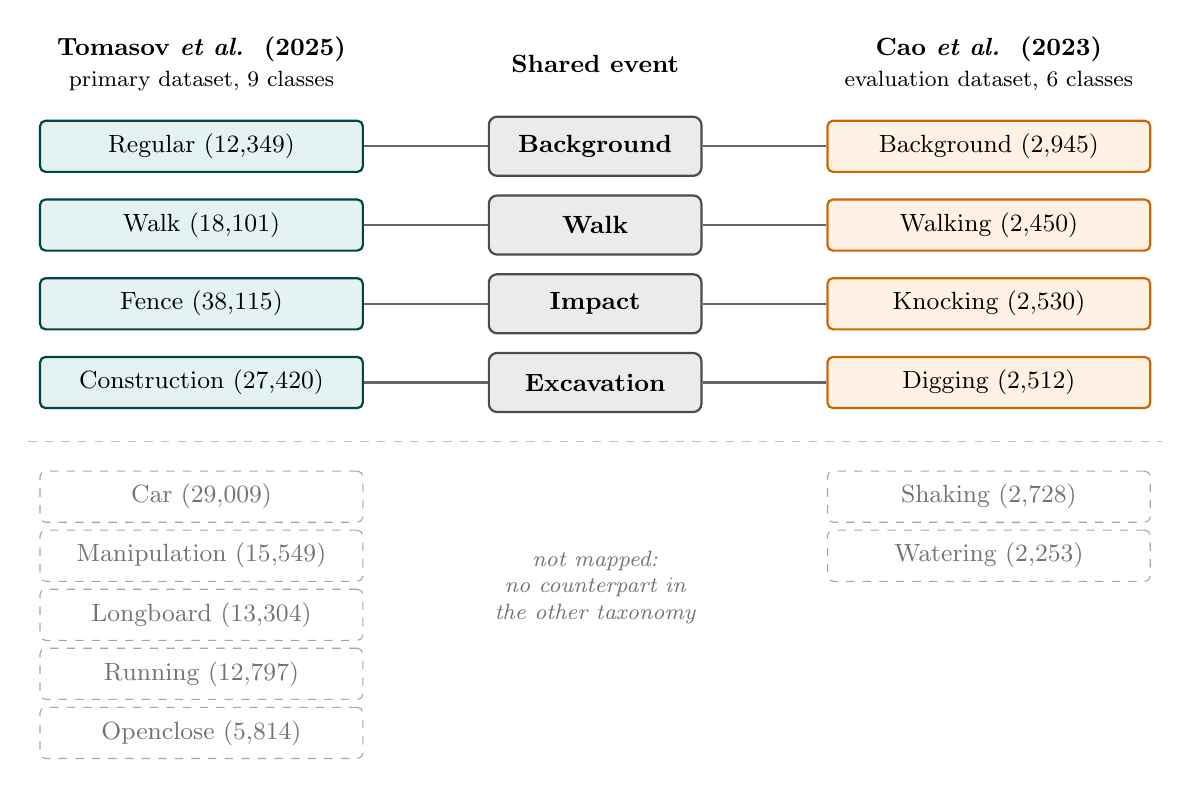
\begin{tikzpicture}[
	font=\small,
	cls/.style={rounded corners=2pt, minimum width=4.1cm, minimum height=6.5mm, inner sep=2pt, align=center, thick},
	tomC/.style={cls, draw=teal!55!black, fill=teal!10},
	caoC/.style={cls, draw=orange!80!black, fill=orange!10},
	harm/.style={draw=black!70, fill=black!8, thick, rounded corners=3pt, minimum width=2.7cm, minimum height=7.5mm, font=\small\bfseries},
	off/.style={cls, thin, draw=black!35, dashed, text=black!55, fill=white},
	link/.style={thick, black!60},
	hdr/.style={font=\small\bfseries, align=center},
]
\foreach \y/\t/\h/\c [count=\i] in {0/Regular (12{,}349)/Background/Background (2{,}945), -1/Walk (18{,}101)/Walk/Walking (2{,}450), -2/Fence (38{,}115)/Impact/Knocking (2{,}530), -3/Construction (27{,}420)/Excavation/Digging (2{,}512)} {
	\node[tomC] (t\i) at (0,\y) {\t};
	\node[harm] (h\i) at (5,\y) {\h};
	\node[caoC] (c\i) at (10,\y) {\c};
	\draw[link] (t\i.east) -- (h\i.west);
	\draw[link] (h\i.east) -- (c\i.west);
}
\draw[black!25, dashed] (-2.2,-3.75) -- (12.2,-3.75);
\foreach \y/\t [count=\i] in {-4.45/Car (29{,}009), -5.2/Manipulation (15{,}549), -5.95/Longboard (13{,}304), -6.7/Running (12{,}797), -7.45/Openclose (5{,}814)} {
	\node[off] (tu\i) at (0,\y) {\t};
}
\foreach \y/\t [count=\i] in {-4.45/Shaking (2{,}728), -5.2/Watering (2{,}253)} {
	\node[off] (cu\i) at (10,\y) {\t};
}
\node[font=\footnotesize\itshape, text=black!55, align=center] at (5,-5.6) {not mapped:\\no counterpart in\\the other taxonomy};
\node[hdr] at (0,1.05) {Tomasov \etal\ (2025)\\{\footnotesize\normalfont primary dataset, 9 classes}};
\node[hdr] at (5,1.05) {Shared event};
\node[hdr] at (10,1.05) {Cao \etal\ (2023)\\{\footnotesize\normalfont evaluation dataset, 6 classes}};
\end{tikzpicture}
\caption{Mapping between the Tomasov and Cao event taxonomies. Four classes on each side map one-to-one onto a shared event type; the remaining classes (dashed) have no counterpart and are excluded from the cross-system tests. Numbers in brackets are Tomasov windows in the final partition and Cao records.}
\label{fig:label_mapping}
\end{figure}

\begin{table}[!htbp]
	\centering
	\caption{Shared event types of the Tomasov and Cao datasets, the physical mechanism behind each, and the samples each covers. Tomasov counts are windows in the final partition; Cao counts are records.}
	\label{tab:label_mapping}
	\small
	\setlength{\tabcolsep}{4pt}
	\begin{tabularx}{\textwidth}{@{}l >{\raggedright\arraybackslash}X l r l r@{}}
		\toprule
		\textbf{Shared event} & \textbf{Mechanism at the fibre} & \textbf{Tomasov} & \textbf{Windows} & \textbf{Cao} & \textbf{Records}\\
		\midrule
		Background  & Ambient state, no target event & Regular      & 12{,}349 & Background & 2{,}945\\
		Walk        & Pedestrian footfall & Walk         & 18{,}101 & Walking    & 2{,}450\\
		Impact      & Impulsive strikes through a structure or the ground & Fence        & 38{,}115 & Knocking   & 2{,}530\\
		Excavation  & Ground worked by machinery or tools & Construction & 27{,}420 & Digging    & 2{,}512\\
		\midrule
		Mapped      & & 4 of 9 classes & 95{,}985 & 4 of 6 classes & 10{,}437\\
		Not mapped  & & 5 classes      & 76{,}473 & 2 classes      & 4{,}981\\
		\bottomrule
	\end{tabularx}
\end{table}

The mapping covers $95{,}985$ of the $172{,}458$ Tomasov windows ($55.7\%$) and $10{,}437$ of the $15{,}418$ Cao records ($67.7\%$). Seven classes are excluded. \emph{Car} and \emph{longboard} are vehicle events with no Cao counterpart. \emph{Running} also consists of footfall, but merging it into \emph{walk} would alter the composition of a class that already has a direct counterpart, for which reason it was excluded rather than merged. \emph{Manipulation} and \emph{openclose} describe interference with the installation at a manhole on the route, for which the Cao setup has no equivalent, and the Cao classes \emph{shaking} and \emph{watering} have no equivalent among the Tomasov classes.

\subsection{Performance on the Shared Classes}
\label{sec:resMappingWithin}
\autoBookmark{subsec}{Performance on the Shared Classes}
Restricting each dataset to its four mapped classes provides a within-system reference (Table~\ref{tab:transfer}). Using only the 941 non-spatial features, LightGBM trained on the $81{,}645$ Tomasov training windows of the four classes and tested on the $6{,}987$ test windows of the frozen partition reaches $73.02\%$ accuracy and a macro-$F_1$ of $70.01$. On Cao, with $7{,}888$ training and $1{,}451$ test records, it reaches $95.93\%$ and $94.45$. The Tomasov reference is lower than the nine-class headline because the spatial block is excluded: without it the nine-class macro-$F_1$ falls to $62.13$ (\refss{sec:resLODO}), and the four shared classes, at $70.01$, lie between the two values. Within each system, the shared events can thus be recognised from signal-agnostic features alone, which is the precondition for a meaningful transfer test.

\subsection{Cross-System Transfer}
\label{sec:resTransfer}
\autoBookmark{subsec}{Cross-System Transfer}
Training on every mapped window of one system and testing on every mapped window of the other yields accuracies below the $25\%$ chance level in both directions: $14.41\%$ when the model is trained on Cao and tested on Tomasov, and $19.12\%$ in the reverse direction (Table~\ref{tab:transfer}). Balanced accuracy, at $21.66\%$ and $20.02\%$, is likewise below chance, which shows that the failure is not an artefact of the class proportions.

\begin{table}[!htbp]
	\centering
	\caption{Within-system and cross-system performance on the four shared event types, using the 941 time, frequency, and time--frequency features. Chance accuracy is $25\%$.}
	\label{tab:transfer}
	\small
	\begin{tabular}{@{}lrrrrr@{}}
		\toprule
		\textbf{Training $\rightarrow$ test} & \textbf{Train} & \textbf{Test} & \textbf{Acc. (\%)} & \textbf{Bal. acc. (\%)} & \textbf{Macro-$F_1$}\\
		\midrule
		Tomasov $\rightarrow$ Tomasov (within) & 81{,}645 & 6{,}987  & 73.02 & 69.29 & 70.01\\
		Cao $\rightarrow$ Cao (within)         & 7{,}888  & 1{,}451  & 95.93 & 94.57 & 94.45\\
		\midrule
		Cao $\rightarrow$ Tomasov              & 10{,}437 & 95{,}985 & 14.41 & 21.66 & 12.97\\
		Tomasov $\rightarrow$ Cao              & 95{,}985 & 10{,}437 & 19.12 & 20.02 & 15.99\\
		\bottomrule
	\end{tabular}
\end{table}

\reff{fig:cross_system} shows the manner in which the transferred models fail. When trained on Cao, the model assigns most Tomasov windows of every class to \emph{background} (from $59.8\%$ of true background to $78.0\%$ of true excavation) and never predicts \emph{impact}, so its recall is $59.8\%$ on background, $17.1\%$ on excavation, $9.7\%$ on walk, and zero on impact. When trained on Tomasov, the model assigns most Cao records to \emph{impact} or \emph{walk}: $80.5\%$ of background records are classified as impact, and $79.0\%$ of excavation and $71.5\%$ of impact records are classified as walk. It never predicts \emph{background}, and its highest recall is $47.1\%$ on walk. Each model collapses the data of the other system onto one or two of its own classes, which is characteristic of a covariate shift so large that the feature distributions of the two systems scarcely overlap even after quantile normalisation.

\begin{figure}[!htbp]
\centering
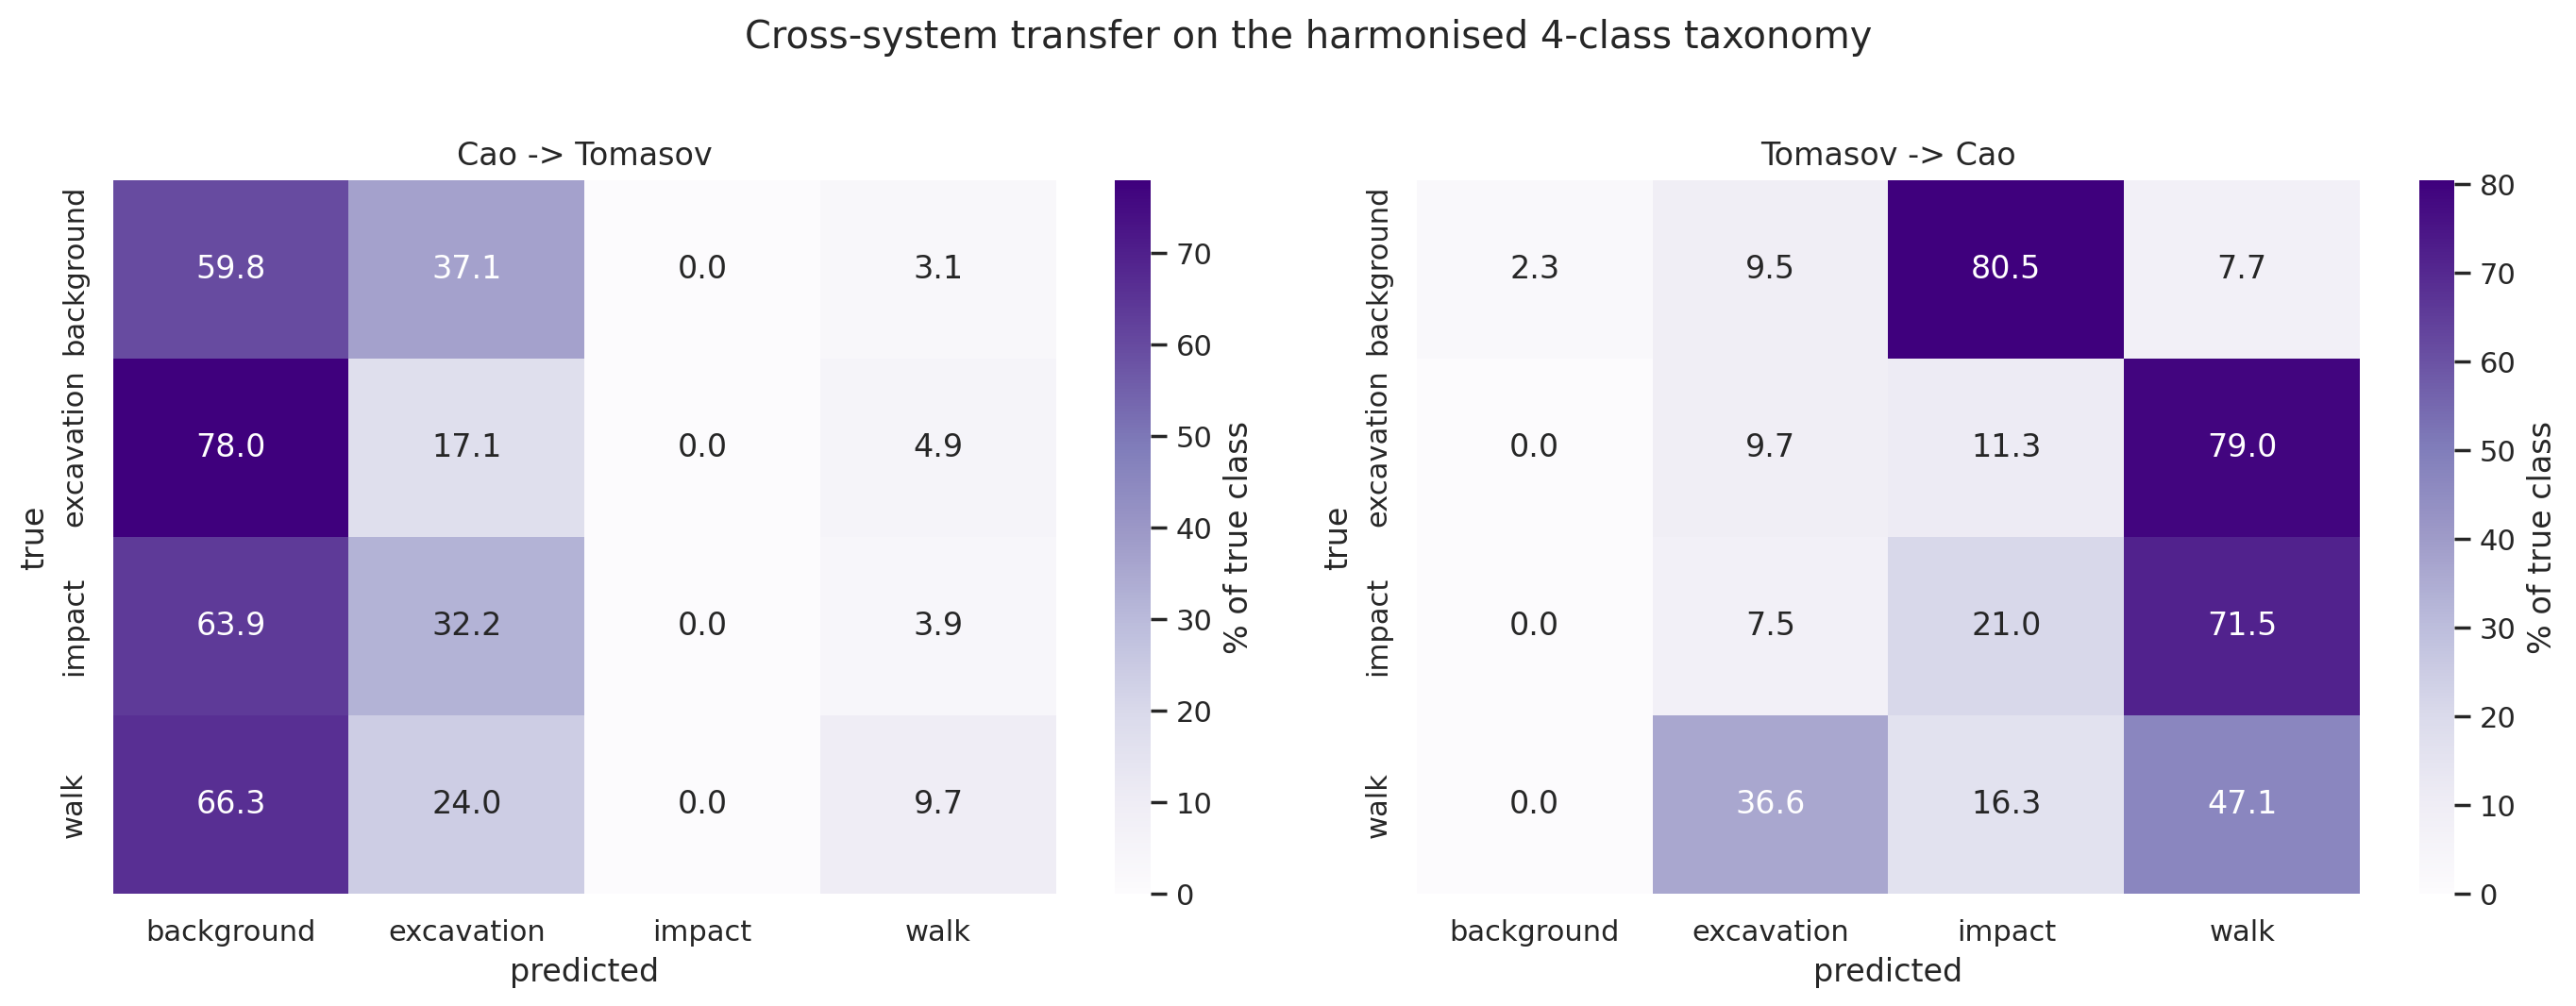
\includegraphics[width=0.95\textwidth,keepaspectratio]{Figures/fig35_cross_system_confusion.png}
\caption{Row-normalised confusion matrices for direct cross-system transfer on the four shared event types: trained on Cao and tested on Tomasov (left), and trained on Tomasov and tested on Cao (right).}
\label{fig:cross_system}
\end{figure}

\subsection{Implications of the Mapping for Generalisability}
\label{sec:resMappingVerdict}
\autoBookmark{subsec}{Implications of the Mapping for Generalisability}
The mapping converts an imprecise question, whether the pipeline generalises across DAS systems, into a measurable one, and the answer depends on the sense in which generalisation is understood. The pipeline as a method transfers: the same configuration, without per-dataset tuning, recognises the shared events well within each system, ranks the feature domains almost identically on both ($\rho = 0.90$), and outperforms the baselines on both (\refs{sec:resDiscussion}). A fitted model does not transfer: when trained on one system, it performs below chance on the other. Two explanations cannot be distinguished with these data. The shared event types may not be physically equivalent across the two installations (construction machinery and manual digging differ greatly in energy and duration, and a fence strike reaches the cable through a different path from a knock on the ground), or the intensity-based and phase-sensitive interrogators may record the same disturbance so differently that quantile normalisation cannot align them. In either case, the deployment of a fitted model on a new interrogator requires labelled data from that interrogator or explicit domain adaptation; adaptation is a prerequisite rather than a refinement. The mapping also provides future work with an established benchmark, since any adaptation method can be evaluated on exactly these four classes in both directions. This negative result completes the generalisation part of \textbf{RQ3}.

\section{Computational Efficiency and Lightweight Footprint}
\label{sec:resEfficiency}
\autoBookmark{sec}{Computational Efficiency and Lightweight Footprint}
Computational cost determines whether the workflow can be executed at the location where a DAS system is deployed, and this section answers \textbf{RQ1}. \refss{sec:resRealTime} decomposes the per-window cost of the pipeline into its stages and compares it with the real-time budget, and \refss{sec:resFootprint} compares the complete footprint of the pipeline with that of every baseline, using the four measures of \refss{sec:chap3Efficiency}.

\subsection{Per-Window Cost and the Real-Time Budget}
\label{sec:resRealTime}
\autoBookmark{subsec}{Per-Window Cost and the Real-Time Budget}
Table~\ref{tab:efficiency} separates the stages of the per-window online cost, measured on the CPU of the Jetson AGX Orin. Classifier inference is sub-millisecond on both datasets and negligible in relation to the window-arrival interval. Feature extraction dominates the cost, and within it the time--frequency domain accounts for approximately $60$\,ms per window, owing to the wavelet-packet decomposition over 16 sub-bands and the grey-level co-occurrence computation. For Tomasov, the total of $144.59$\,ms exceeds the window-arrival interval of $102.4$\,ms, and two cores are consequently required for real-time processing of a single channel. For Cao, the total of $122.54$\,ms fits within the interval of $204.8$\,ms on one core. Feature selection is a one-time offline cost; Boruta is the most expensive method at $665$\,s (Tomasov) and $745$\,s (Cao), and the filter methods complete in under five seconds. Preprocessing is negligible relative to extraction, as anticipated in \refss{sec:chap3PreprocCost}.

\begin{table}[!htbp]
	\centering
	\caption{Computational cost per window and the real-time budget.}
	\label{tab:efficiency}
	\small
	\begin{tabular}{@{}lrr@{}}
		\toprule
		\textbf{Stage} & \textbf{Tomasov (ms)} & \textbf{Cao (ms)}\\
		\midrule
		Time-domain extraction        & 43.16 & 42.62\\
		Frequency-domain extraction   & 3.35  & 3.34\\
		Time--frequency extraction    & 60.67 & 59.49\\
		Spatial extraction            & 37.40 & 17.10\\
		\midrule
		\textbf{Total extraction}     & \textbf{144.59} & \textbf{122.54}\\
		Classifier inference          & 0.17  & 0.06\\
		\midrule
		Window arrival interval       & 102.4 & 204.8\\
		Cores required for real time  & 2     & 1\\
		\bottomrule
	\end{tabular}
\end{table}

\subsection{Lightweight Footprint of the Pipeline and the Baselines}
\label{sec:resFootprint}
\autoBookmark{subsec}{Lightweight Footprint of the Pipeline and the Baselines}
Table~\ref{tab:footprint} compares the four footprint measures of the pipeline with those of the two published CNNs and the five recent architectures, all trained on the same leakage-controlled partitions and timed on the same board. The feature pipeline runs on the CPU cores of the board, whereas every network was trained and executed on its integrated GPU. The two LightGBM sizes are obtained by counting the split thresholds, split features, and leaf values of the fitted boosters, and refitting the selected configurations under the fixed seed reproduces their reported test metrics exactly. The native text model file of LightGBM, which also stores split gains and node counts, is larger: $32.8$\,MB on Tomasov and $8.5$\,MB on Cao, or $14.7$ and $3.5$\,MB when compressed.

\begin{table}[!htbp]
	\centering
	\caption[Lightweight footprint of the pipeline and every baseline]{Lightweight footprint of the feature pipeline and every baseline on the Jetson AGX Orin, on the leakage-controlled partitions. Size counts stored parameters at 32 bits each (\refss{sec:chap3Efficiency}). Latencies are per window and amortised over the test set; end-to-end latency adds the preparation of each model's input. n.r.: not recorded.}
	\label{tab:footprint}
	\footnotesize
	\setlength{\tabcolsep}{3.5pt}
	\resizebox{\textwidth}{!}{%
	\begin{tabular}{@{}llrrrrr@{}}
		\toprule
		\textbf{Model} & \textbf{Processor} & \textbf{Parameters} & \textbf{Size (MB)} & \textbf{Training (s)} & \textbf{Inference (ms)} & \textbf{End-to-end (ms)}\\
		\midrule
		\multicolumn{7}{@{}l}{\textit{Tomasov \etal\ 2025}}\\[2pt]
		Pipeline, $1{,}002$ feat.\ (proposed) & CPU & 855{,}000 & 3.42 & 1{,}357 & 0.17 & 144.77\\
		Pipeline, 52 feat.\ (proposed) & CPU & 855{,}000 & 3.42 & \textbf{63} & 0.15 & 144.74$^{a}$\\
		Tomasov CNN, dense 1024~\cite{tomasov2025perimeter} & GPU & 33{,}155{,}849 & 132.62 & 1{,}569 & n.r. & n.r.\\
		Tomasov CNN, dense 256~\cite{tomasov2025perimeter}  & GPU & 8{,}375{,}561 & 33.50 & 1{,}103 & n.r. & n.r.\\
		DAStatFormer~\cite{dione2026dastatformer} & GPU & 16{,}077{,}327 & 64.31 & 32{,}958 & 0.62 & $\geq 0.62^{b}$\\
		DASViT1D~\cite{dione2025intrusion}        & GPU & 1{,}655{,}561 & 6.62 & 1{,}184 & \textbf{0.16} & $\geq 0.16^{b}$\\
		S2-DyGNN~\cite{jeong2026s2dygnn}          & GPU & 56{,}329 & 0.23 & 25{,}530 & 5.67 & 5.67\\
		GAT~\cite{jeong2026s2dygnn,shahabudin2024gnn} & GPU & 52{,}361 & 0.21 & 25{,}135 & 5.08 & 5.08\\
		GCN~\cite{jeong2026s2dygnn,shahabudin2024gnn} & GPU & 48{,}137 & \textbf{0.19} & 37{,}704 & 5.16 & 5.16\\
		\midrule
		\multicolumn{7}{@{}l}{\textit{Cao \etal\ 2023}}\\[2pt]
		Pipeline, $1{,}002$ feat.\ (proposed) & CPU & 208{,}578 & 0.83 & 41 & \textbf{0.06} & 122.60\\
		Pipeline, 53 feat.\ (proposed) & CPU & 357{,}390 & 1.43 & \textbf{8} & 0.07 & 122.61$^{a}$\\
		Cao CNN~\cite{caoxin2023opendataset} & GPU & 7{,}421 & \textbf{0.03} & 628 & n.r. & n.r.\\
		DAStatFormer~\cite{dione2026dastatformer} & GPU & 15{,}985{,}164 & 63.94 & 1{,}775 & 0.76 & $\geq 0.76^{b}$\\
		DASViT1D~\cite{dione2025intrusion}        & GPU & 1{,}655{,}174 & 6.62 & 130 & 0.19 & $\geq 0.19^{b}$\\
		S2-DyGNN~\cite{jeong2026s2dygnn}          & GPU & 56{,}134 & 0.22 & 1{,}392 & 3.75 & 3.75\\
		GAT~\cite{jeong2026s2dygnn,shahabudin2024gnn} & GPU & 52{,}166 & 0.21 & 2{,}063 & 3.10 & 3.10\\
		GCN~\cite{jeong2026s2dygnn,shahabudin2024gnn} & GPU & 47{,}942 & 0.19 & 2{,}531 & 3.03 & 3.03\\
		\bottomrule
	\end{tabular}}
	\par\smallskip
	\begin{minipage}{\textwidth}\scriptsize
	Pipeline: LightGBM on the full or the consensus feature set. $^{a}$\,The extractor computes every domain in full, so the consensus configuration pays the full extraction cost. $^{b}$\,Excludes computing the model's input features (MFCC, RDFT, and DWT for DASViT1D; 24 statistics per channel for DAStatFormer), which were computed in advance and not timed. The graph models compute their STFT inside the timed forward pass, so their figure is end-to-end apart from the band-pass and z-score conditioning they share with the pipeline.
	\end{minipage}
\end{table}

The four measures rank the models differently, which is the reason why all four are required. In \emph{model size}, the $3.42$\,MB of the pipeline on Tomasov is a nineteenth of the size of DAStatFormer ($64.31$\,MB), a tenth to a thirty-ninth of that of the reconstructed Tomasov CNN ($33.50$--$132.62$\,MB), and half of that of DASViT1D ($6.62$\,MB), but fifteen to eighteen times the size of the three graph networks, each of which holds about fifty thousand weights; on Cao the same ordering holds at $0.83$\,MB, with the $7{,}421$-weight Cao CNN the smallest model overall. In \emph{inference latency}, the CPU classifier of the pipeline ($0.17$ and $0.06$\,ms) matches the fastest network on its GPU, DASViT1D, on Tomasov ($0.16$\,ms) and is three times faster on Cao ($0.19$\,ms); it is four to twelve times faster than DAStatFormer and thirty to sixty times faster than the graph networks. In \emph{training cost}, the pipeline requires $1{,}357$\,s on Tomasov and $41$\,s on Cao on CPU cores, against $1{,}103$--$37{,}704$\,s and $130$--$2{,}531$\,s of GPU time for the networks; only DASViT1D and the smaller Tomasov CNN train faster on Tomasov, and the consensus configuration trains in $63$ and $8$\,s, faster than every network on both datasets. In \emph{end-to-end latency}, the order is reversed. Feature extraction brings the online cost of the pipeline to $122.60$--$144.77$\,ms per window, compared with $3.03$--$5.67$\,ms for the graph networks, and the cost of computing the input features of the transformers was not timed.

These measurements answer RQ1. A DAS classifier is lightweight in the sense of \refs{sec:ResearchBackground} when its learning stage is small, requires no GPU, and trains within minutes, and when its complete online cost fits within the window-arrival interval on a few CPU cores of the board located beside the interrogator. The feature pipeline satisfies that definition: a model of $0.8$--$3.4$\,MB, CPU-only training in under $23$ minutes (about one minute with consensus selection), sub-millisecond CPU inference, and an online cost that fits within the window interval on one core for Cao and two for Tomasov. It is not, however, the lightest model on every measure. The graph networks are smaller and, given a GPU, less costly per window, but each requires seven to ten and a half hours of GPU training on Tomasov, and their decisions cannot be traced to named quantities (\refss{sec:resWhiteBox}). The lightness of the pipeline therefore lies in its learning stage and its hardware requirements, and its most expensive component is feature extraction, in which further savings should be sought (\refss{sec:chap5FutureCost}). Real-time claims based on inference latency alone would omit that principal online cost, and for this reason the end-to-end figure is reported for every model.
\section{Discussion}
\label{sec:resDiscussion}
\autoBookmark{sec}{Discussion}
This section relates the preceding results to the prior work on which they build. The baseline branch of \reff{fig:methodology_framework} trains the CNN published with each dataset and five recent architectures on raw windows, or on the input features their designs compute from them, drawn from the same partitions as the feature pipeline, and scores them with the same metrics on the same test windows, so that every difference reported in this section is attributable to the models and the evaluation protocols rather than to the data. The aim is to establish how, and why, the findings of this study differ from the accuracies reported in the source publications. \refss{sec:resCNN} compares the pipeline with the published CNNs; \refss{sec:resCapacity} and \refss{sec:resReproGap} use those networks to measure the sensitivity of a single architecture to leakage; \refss{sec:resSOTA} extends the comparison to five architectures published from 2024 onwards, with the size and latency of every model; \refss{sec:resWhiteBox} contrasts the white-box pipeline with the black-box networks; and \refss{sec:resSynthesis} synthesises the comparisons.

\subsection{Comparison with the Published CNN Baselines}
\label{sec:resCNN}
\autoBookmark{subsec}{Comparison with the Published CNN Baselines}
Table~\ref{tab:cnn_comparison} compares the feature pipeline with the CNN published with each dataset, trained on identical leakage-controlled partitions as specified in \refss{sec:chap3Baselines}. The pipeline leads by $16.43$ macro-$F_1$ points on Tomasov and $8.01$ on Cao, which answers the comparative part of \textbf{RQ3} for the published baselines. The partitions are identical across models, but the inputs are not: the feature pipeline operates on demeaned, band-passed, z-scored windows, whereas each CNN is reproduced on the raw records that its source publication assumes. Under the operational rates defined with the Cao dataset, its CNN attains a nuisance-alarm rate of $0.45\%$ and a false-negative rate of $0.89\%$ on the session-grouped partition; equivalent rates were not computed for the feature pipeline and are not claimed.

\begin{table}[!htbp]
	\centering
	\caption[Feature pipeline compared with the CNN baselines]{Feature pipeline compared with the CNN baselines, and the protocol sensitivity of the reconstructed Tomasov CNN. Parameters are trainable weights for the CNNs and stored split and leaf values for LightGBM; size counts them at 32 bits each. Latency is per window on the Jetson AGX Orin, given for the pipeline as classifier inference / end-to-end including feature extraction; the CNNs' inference time was not recorded (n.r.). Acc.: accuracy; $\Delta$Acc.: change from the same model on the blocked partition.}
	\label{tab:cnn_comparison}
	\footnotesize
	\setlength{\tabcolsep}{4pt}
	\resizebox{\textwidth}{!}{%
\begin{tabular}{@{}lrrr>{\raggedright\arraybackslash}p{3.2cm}rrr@{}}
		\toprule
		\textbf{Method} & \textbf{Parameters} & \textbf{Size (MB)} & \textbf{Latency (ms)} & \textbf{Partition} & \textbf{Acc. (\%)} & \textbf{Macro-$F_1$} & \textbf{$\Delta$Acc.}\\
		\midrule
		\multicolumn{8}{@{}l@{}}{\emph{Tomasov 2025}}\\
		Multi-domain features, $1{,}002$ & 855\,k & 3.42 & 0.17 / 144.77 & Blocked + guard bands & \textbf{90.71} & \textbf{81.98} & ---\\
		Consensus features, 52           & 855\,k & 3.42 & 0.15 / 144.74 & Blocked + guard bands & 77.29 & 73.59 & ---\\
		Tomasov CNN, reconstructed, dense 1024 & 33.2\,M & 132.62 & n.r. & Blocked + guard bands & 68.74 & 65.55 & ---\\
		Tomasov CNN, reconstructed, dense 256  & 8.4\,M  & 33.50  & n.r. & Blocked + guard bands & 67.28 & 64.66 & ---\\
		\midrule
		\multicolumn{8}{@{}l@{}}{\emph{Protocol sensitivity of the reconstructed Tomasov CNN (dense 1024)}}\\
		Random partition, same windows   & 33.2\,M & 132.62 & n.r. & Random 80/10/10, 2{,}048-sample stride & 69.99 & 69.90 & $+1.25$\\
		Random partition, windows re-cut & 33.2\,M & 132.62 & n.r. & Random 80/10/10, 256-sample stride & 95.01 & 94.64 & $+26.27$\\
		Published~\cite{tomasov2025perimeter}, authors' protocol & Not stated & --- & --- & Random 10-fold, 256-sample stride & 85.47 & 84.84 & ---\\
		\midrule
		\multicolumn{8}{@{}l@{}}{\emph{Cao 2023}}\\
		Multi-domain features, $1{,}002$ & 209\,k & 0.83 & 0.06 / 122.60 & Session-grouped & \textbf{99.06} & \textbf{98.90} & ---\\
		Consensus features, 53           & 357\,k & 1.43 & 0.07 / 122.61 & Session-grouped & 94.40 & 93.08 & ---\\
		Cao CNN~\cite{caoxin2023opendataset} & 7{,}421 & 0.03 & n.r. & Session-grouped & 91.13 & 90.88 & ---\\
		\bottomrule
	\end{tabular}}
\end{table}

\begin{figure}[!htbp]
\centering
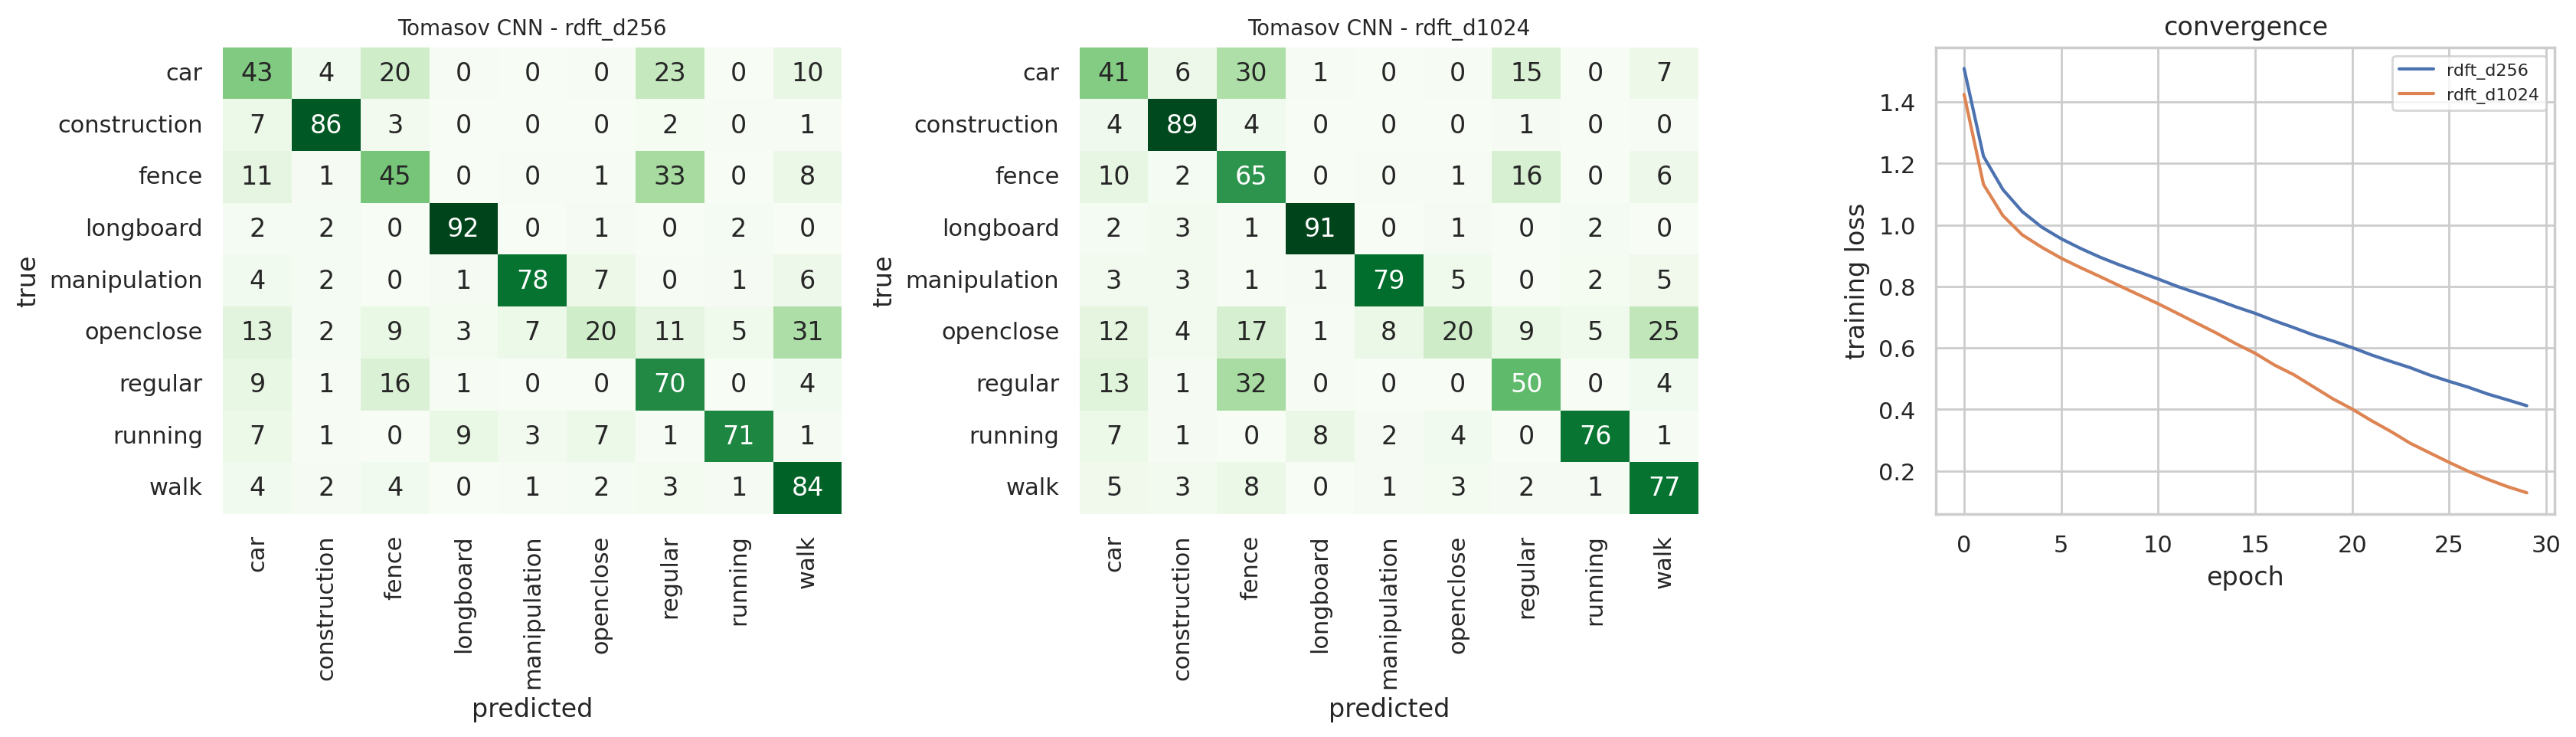
\includegraphics[width=0.98\textwidth,keepaspectratio]{Figures/fig31_tomasov_cnn.png}
\caption{Reconstructed Tomasov CNN on the blocked partition: row-normalised confusion matrices for the 256-unit and $1{,}024$-unit dense layers, and training convergence.}
\label{fig:tomasov_cnn}
\end{figure}

\subsection{Model Capacity and Leakage Sensitivity}
\label{sec:resCapacity}
\autoBookmark{subsec}{Model Capacity and Leakage Sensitivity}
The Cao CNN was trained under both its released partition and the session-grouped partition, which provides a controlled estimate of the extent to which that architecture exploits leakage. Accuracy decreases from $92.70\%$ to $91.13\%$ and macro-$F_1$ from $92.47$ to $90.88$, reductions of only $1.58$ and $1.59$ points despite the near-total contamination documented in \refs{sec:resLeakage}. \reff{fig:cao_cnn} shows the confusion matrices and convergence under both protocols.

\begin{figure}[!htbp]
\centering
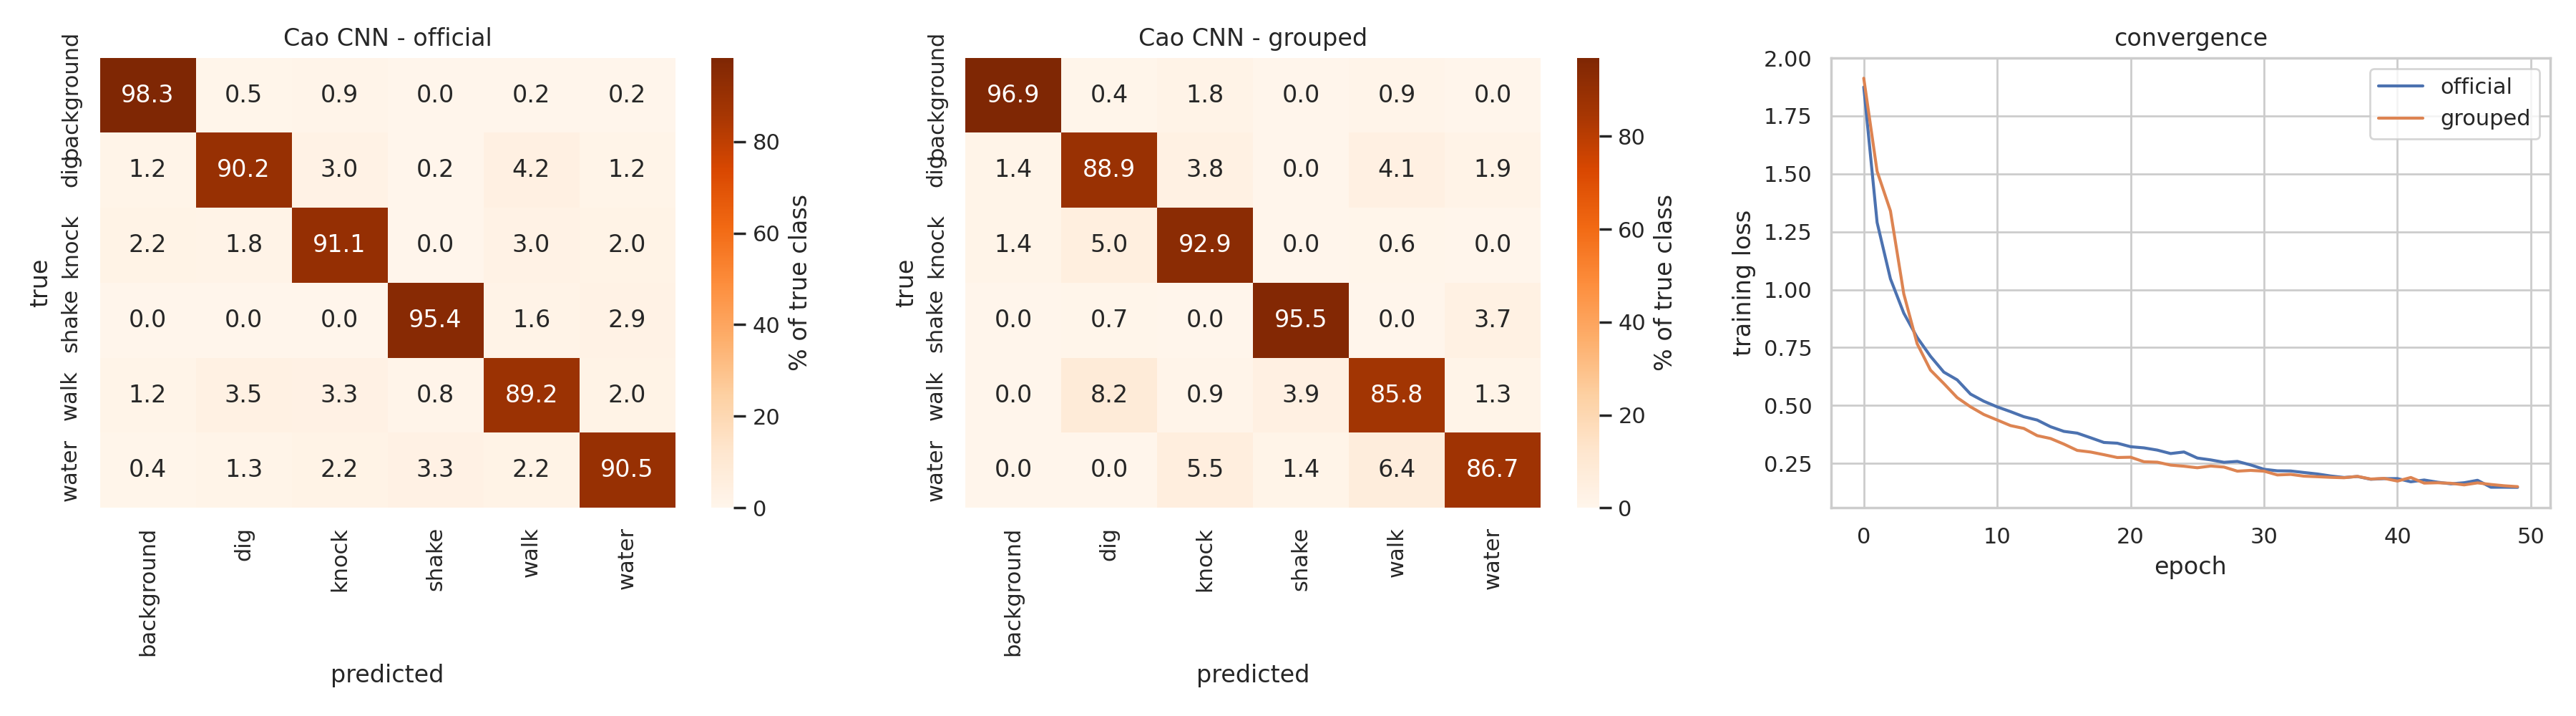
\includegraphics[width=0.95\textwidth,keepaspectratio]{Figures/fig25_cao_cnn.png}
\caption{Cao CNN under both protocols: confusion matrices and training convergence.}
\label{fig:cao_cnn}
\end{figure}

Model capacity is one plausible explanation. With $7{,}421$ parameters, this network has far less capacity than a $1{,}002$-feature gradient-boosted ensemble and may be less able to exploit recording-specific structure. On this account, leakage does not affect all models equally and may favour higher-capacity models, so model rankings obtained under contaminated protocols need not agree with rankings obtained under group-aware evaluation. \refss{sec:resSOTA} tests this hypothesis across five further architectures.

\subsection{Protocol Attribution for the Tomasov CNN}
\label{sec:resReproGap}
\autoBookmark{subsec}{Protocol Attribution for the Tomasov CNN}
The reconstructed Tomasov CNN attains $68.74\%$ accuracy under the blocked partition, compared with the $85.47\%$ reported by its authors. The attribution of that gap requires that one variable be changed at a time, and the network was accordingly trained three times with the architecture, seed, front end, and training recipe fixed and only the partition varied (\reff{fig:protocol_attribution}). Under a random partition of the same $2{,}048$-hop windows it reaches $69.99\%$, a gain of $1.25$ points. Under a random partition of windows re-cut at the 256-sample stride of the authors, which reproduces their window density, it reaches $95.01\%$: $26.27$ points above the blocked partition and $25.02$ above the random partition at the coarser stride. The protocol alone therefore accounts for $26.27$ accuracy points on an otherwise identical model, and the inflation is driven by the density of the overlap rather than by the randomness of the assignment. At $75\%$ overlap a random split adds $1.25$ points; at $96.9\%$ it adds $26.27$.

\begin{figure}[!htbp]
\centering
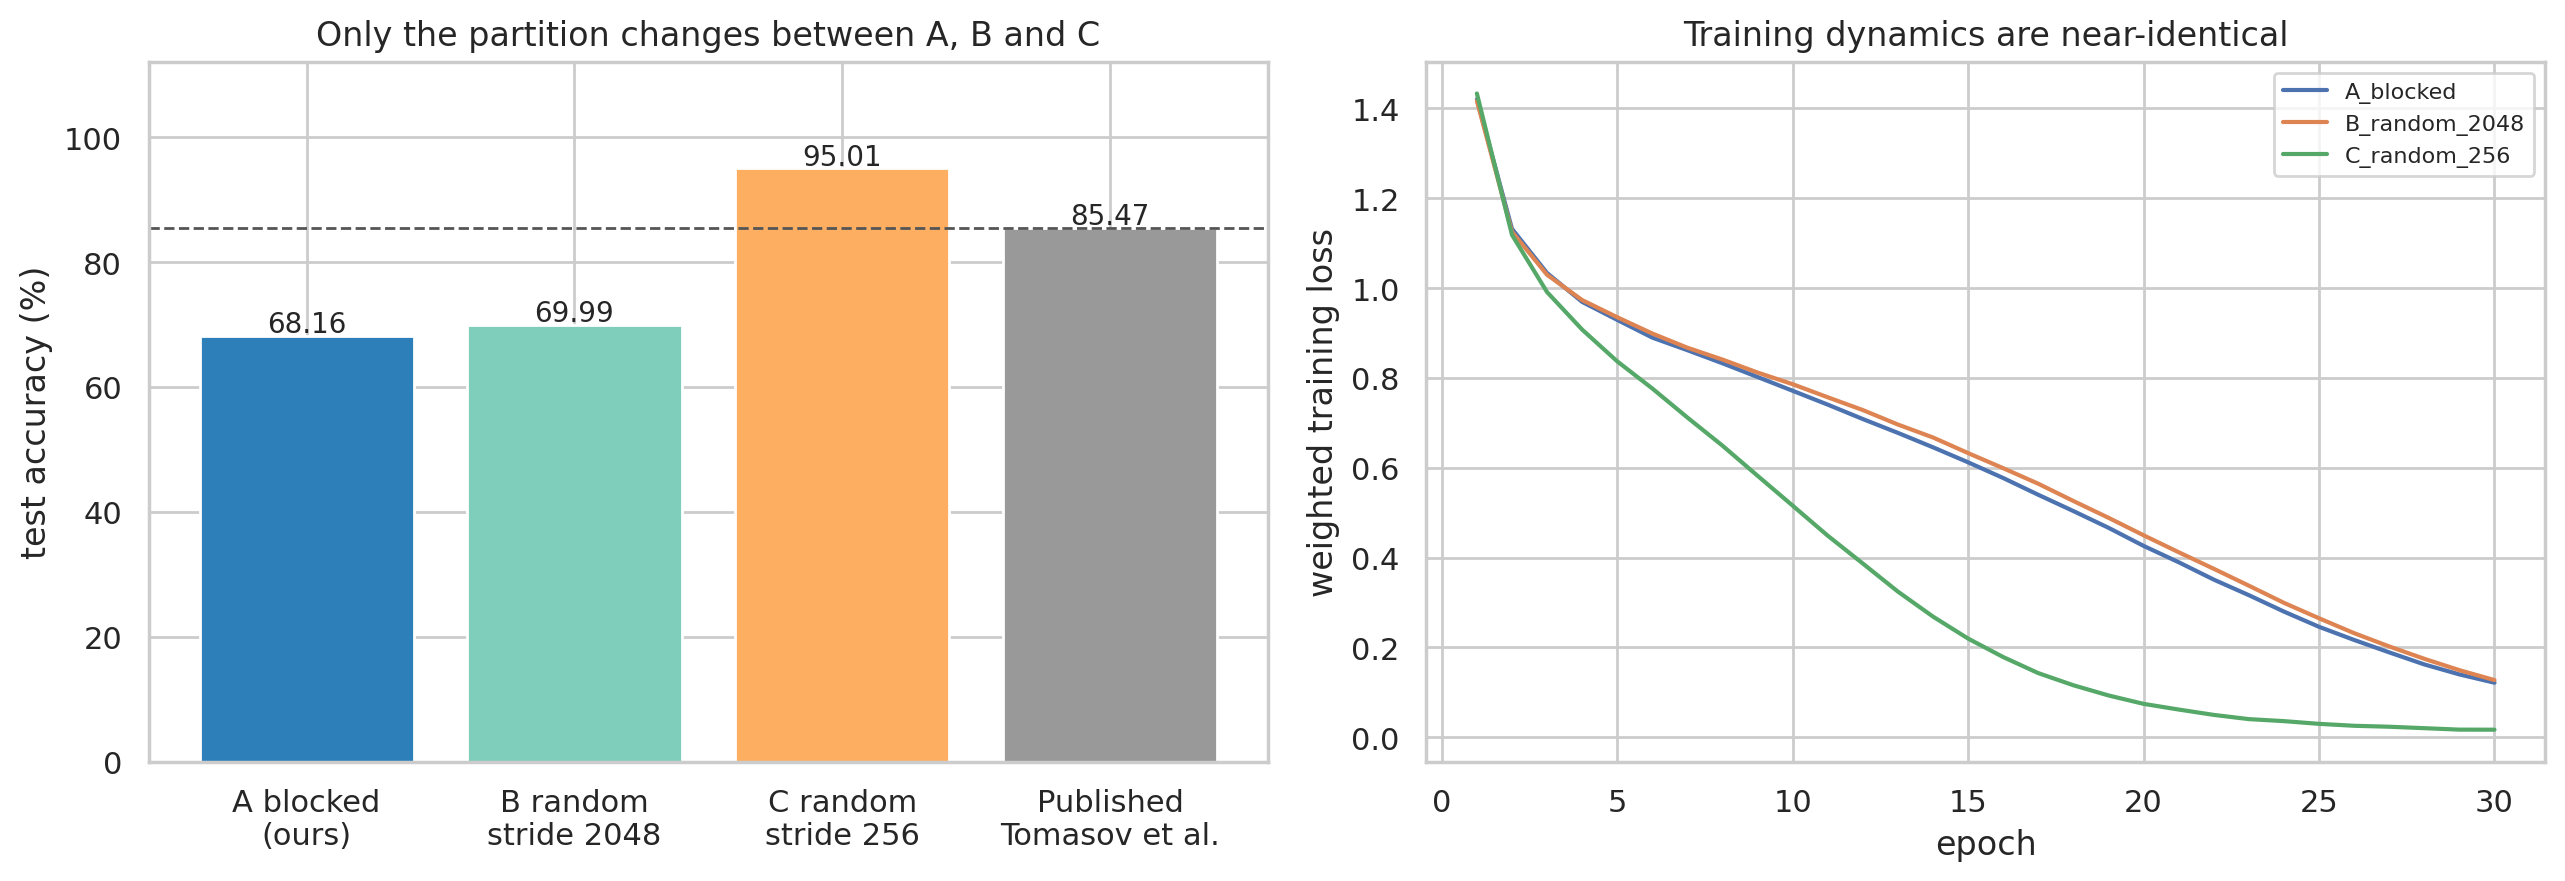
\includegraphics[width=0.98\textwidth,keepaspectratio]{Figures/fig32_protocol_attribution.png}
\caption{Protocol attribution for the reconstructed Tomasov CNN. Left: test accuracy under the three arms and the published figure; only the partition differs between arms. Right: weighted training loss per epoch, which is near-identical for arms A and B and collapses under arm C, the signature of memorised near-duplicates. The arm-A bar is from the attribution run and differs from the value in Table~\ref{tab:cnn_comparison} by a few tenths, the run-to-run variation of single CNN trainings on this dataset.}
\label{fig:protocol_attribution}
\end{figure}

The published figure of $85.47\%$ was not reproduced exactly. Under the protocol of the authors the reconstruction achieves $95.01\%$, exceeding the published figure by $9.54$ points, and this discrepancy is reported rather than removed by tuning. The excess is consistent with leakage in the re-cut windows that is at least as strong as in the originals: the final training loss is $0.017$ under arm C against $0.121$ under the leakage-controlled partition. The consequence for the comparison is favourable, but it must be stated precisely. The reconstruction is not a weakened replica, so the $68.74\%$ measured under leakage control cannot be attributed to a poor reimplementation; it is a fair measurement of that architecture under a sample-disjoint protocol. The source specifies a 256-unit dense layer, and the $1{,}024$-unit variant is reported as the reproduction because it scores higher, which means that the comparison is likewise not made against a weakened baseline. The fourfold increase in capacity yields only $0.89$ macro-$F_1$ points.

Two limitations remain. First, the re-cut partition reconstructs the published protocol rather than reproducing it, since it expands a sampled subset of parent windows onto the 256-sample grid, with the result that leakage is dense within clusters whereas the original tiling is continuous. Second, single-run CNN accuracies on this dataset should be interpreted only to the nearest point, because training runs that differ only in row ordering vary by a few tenths.

\subsection{Comparison with Recent Architectures}
\label{sec:resSOTA}
\autoBookmark{subsec}{Comparison with Recent Architectures}
Five architectures published from 2024 onwards were reimplemented and trained under the partitions, preprocessing constraints, and metrics used throughout this thesis (\refss{sec:chap3SOTA}). Table~\ref{tab:sota} reports the results, with the parameter count, stored size, and per-window latency of every model, and \reff{fig:sota} illustrates them. On Tomasov the feature pipeline attains $90.71\%$ accuracy and $81.98$ macro-$F_1$, exceeding the strongest neural baseline by $11.88$ accuracy points and $3.44$ macro-$F_1$ points. On Cao it attains $99.06\%$ and $98.90$, exceeding the strongest neural baseline by $1.11$ and $1.32$. \refss{sec:chap5LimResidue} qualifies the Tomasov margin. The ordering in the published literature is not preserved: S2-DyGNN reports $94.0\%$ accuracy on Tomasov under its own chronological partition and reaches $77.59\%$ under the present protocol, and DAStatFormer reports $99.93\%$ and reaches $78.83\%$.

\begin{table}[!htbp]
	\centering
	\caption[Recent architectures under the leakage-controlled protocol]{Recent architectures under the leakage-controlled protocol, with the size and latency of each model. All models use identical partitions, preprocessing constraints, and metrics. Size counts stored parameters at 32 bits each; latency is per window on the Jetson AGX Orin (CPU for the pipeline, GPU for the networks), given for the pipeline as classifier inference / end-to-end including feature extraction. Published accuracy is each method's own reported figure under its own protocol. Table~\ref{tab:footprint} adds training cost.}
	\label{tab:sota}
	\footnotesize
	\setlength{\tabcolsep}{4pt}
	\resizebox{\textwidth}{!}{%
\begin{tabular}{@{}lrrrrrrrr@{}}
		\toprule
		\textbf{Method} & \textbf{Parameters} & \textbf{Size (MB)} & \textbf{Latency (ms)} & \textbf{Acc. (\%)} & \textbf{Macro-$F_1$} & \textbf{Openclose $F_1$} & \textbf{Published acc.} & \textbf{$\Delta$Acc.}\\
		\midrule
		\multicolumn{9}{@{}l@{}}{\emph{Tomasov 2025, blocked + guard bands}}\\
		Multi-domain features (proposed) & 855\,k & 3.42 & 0.17 / 144.77 & \textbf{90.71} & \textbf{81.98} & 0.044 & --- & ---\\
		DAStatFormer~\cite{dione2026dastatformer} & 16.1\,M & 64.31 & $0.62^{b}$ & 78.83 & 73.27 & 0.115 & 99.93 & $-21.10$\\
		S2-DyGNN~\cite{jeong2026s2dygnn}          & 56\,k   & 0.23 & 5.67 & 77.59 & 78.54 & \textbf{0.625} & 94.0 & $-16.41$\\
		GAT~\cite{jeong2026s2dygnn,shahabudin2024gnn} & 52\,k & 0.21 & 5.08 & 77.33 & 75.28 & 0.278 & 81.2 & $-3.88$\\
		GCN~\cite{jeong2026s2dygnn,shahabudin2024gnn} & 48\,k & 0.19 & 5.16 & 69.61 & 71.03 & 0.433 & 85.3 & $-15.69$\\
		DASViT1D~\cite{dione2025intrusion}        & 1.7\,M  & 6.62 & $0.16^{b}$ & 57.15 & 55.38 & 0.141 & 93.5 & $-36.35$\\
		\midrule
		\multicolumn{9}{@{}l@{}}{\emph{Cao 2023, session-grouped}}\\
		Multi-domain features (proposed) & 209\,k & 0.83 & 0.06 / 122.60 & \textbf{99.06} & \textbf{98.90} & --- & --- & ---\\
		GCN~\cite{jeong2026s2dygnn,shahabudin2024gnn} & 48\,k & 0.19 & 3.03 & 97.95 & 97.58 & --- & --- & ---\\
		DAStatFormer~\cite{dione2026dastatformer} & 16.0\,M & 63.94 & $0.76^{b}$ & 97.67 & 97.30 & --- & 99.48 & $-1.81$\\
		GAT~\cite{jeong2026s2dygnn,shahabudin2024gnn} & 52\,k & 0.21 & 3.10 & 96.28 & 94.72 & --- & --- & ---\\
		S2-DyGNN~\cite{jeong2026s2dygnn}          & 56\,k   & 0.22 & 3.75 & 84.14 & 77.35 & --- & --- & ---\\
		DASViT1D~\cite{dione2025intrusion}        & 1.7\,M  & 6.62 & $0.19^{b}$ & 83.58 & 78.45 & --- & --- & ---\\
		\bottomrule
	\end{tabular}}
	\par\smallskip
	\begin{minipage}{\textwidth}\scriptsize
	$^{b}$\,Inference only; the model's input features were computed in advance and not timed (Table~\ref{tab:footprint}).
	\end{minipage}
\end{table}

\begin{figure}[!htbp]
\centering
\begin{subfigure}[b]{0.48\textwidth}
	\centering
	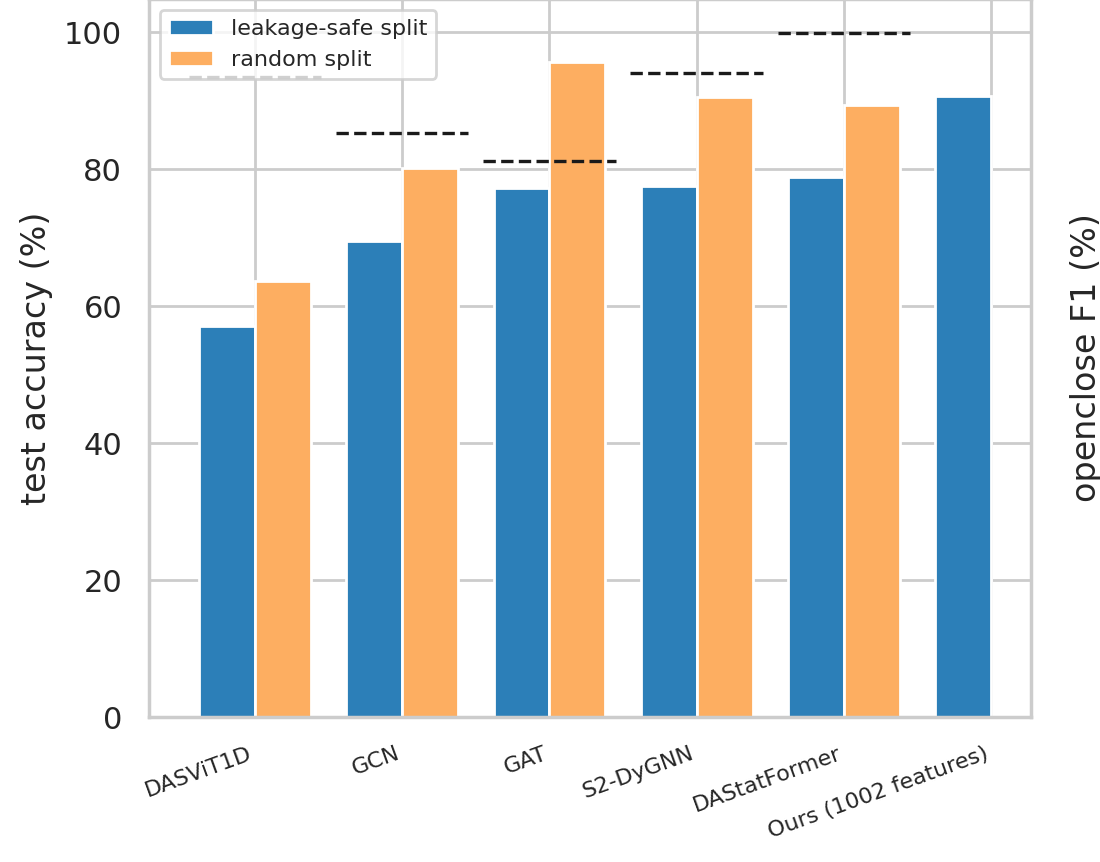
\includegraphics[width=\textwidth,keepaspectratio]{Figures/fig33a_sota_accuracy.png}
	\caption{Test accuracy under both partitions; dashed lines mark each method's published figure.}
\end{subfigure}\hfill
\begin{subfigure}[b]{0.48\textwidth}
	\centering
	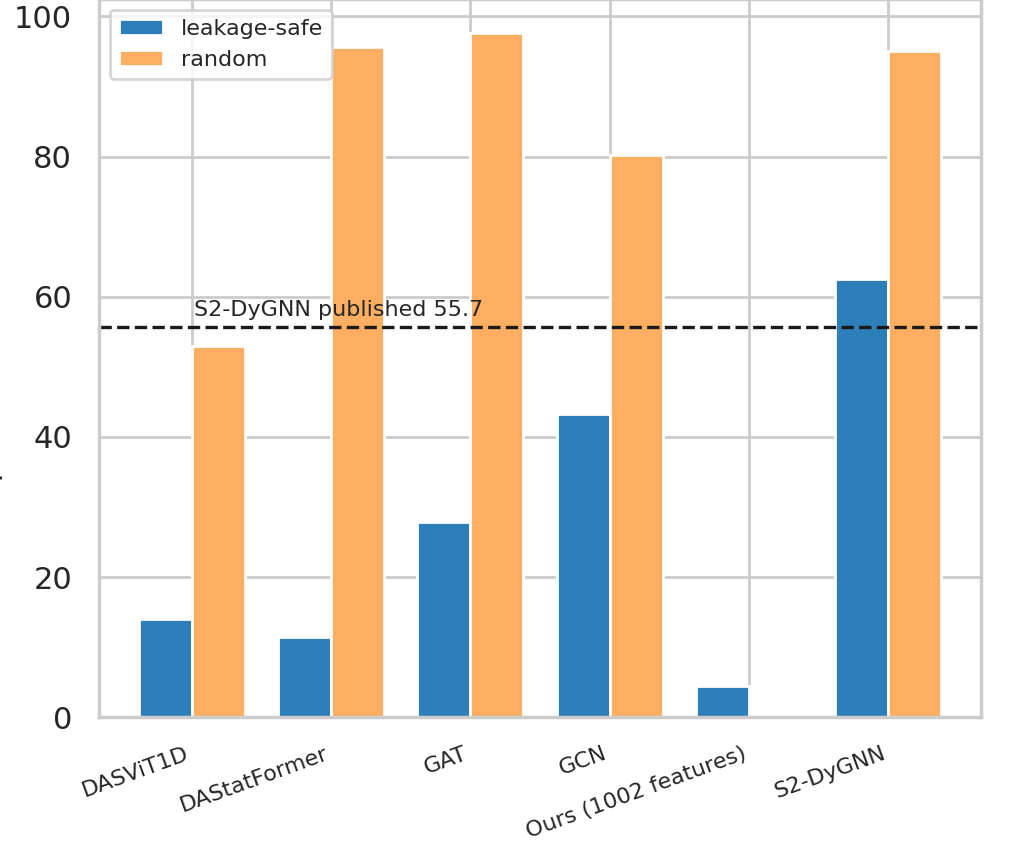
\includegraphics[width=\textwidth,keepaspectratio]{Figures/fig33b_sota_openclose.png}
	\caption{\emph{Openclose} $F_1$ under both partitions.}
\end{subfigure}\\[6pt]
\begin{subfigure}[b]{0.6\textwidth}
	\centering
	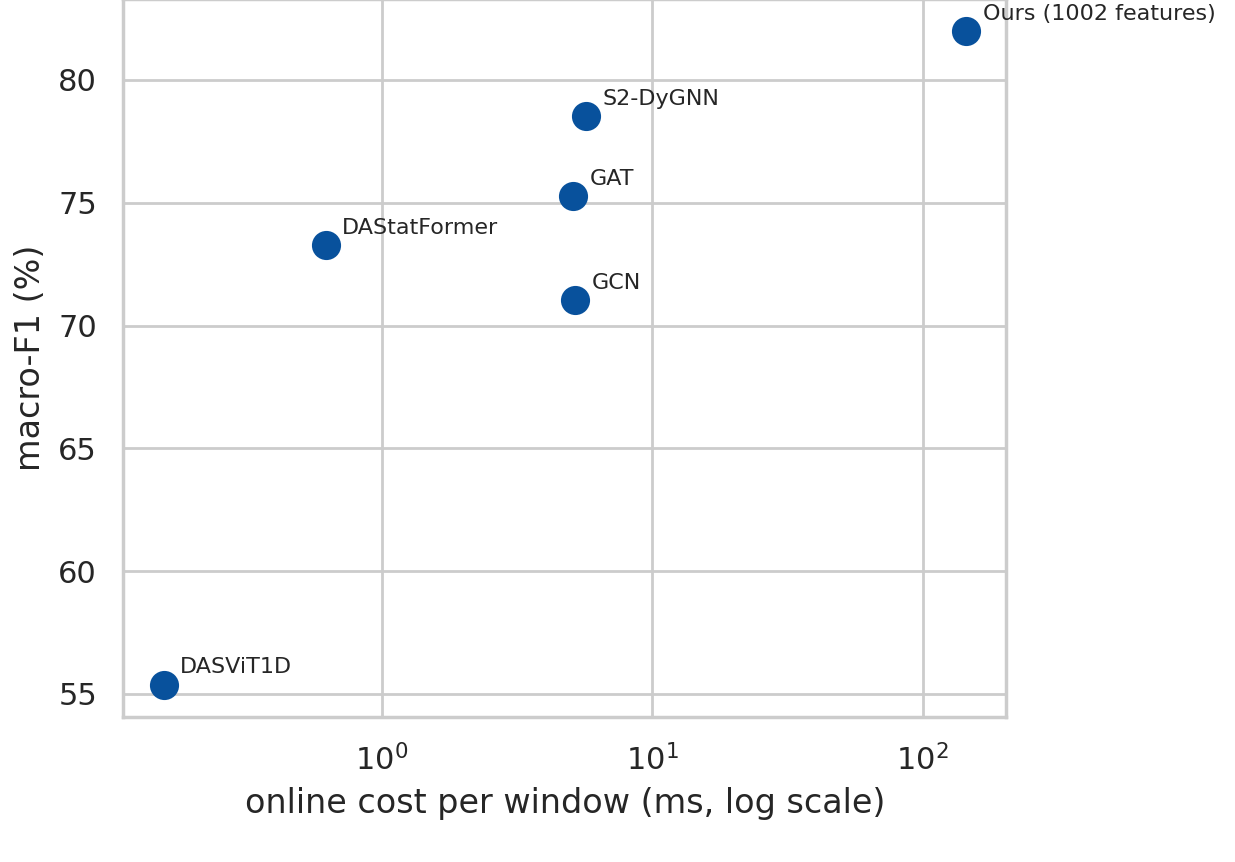
\includegraphics[width=\textwidth,keepaspectratio]{Figures/fig33c_sota_cost.png}
	\caption{Macro-$F_1$ against online cost per window (leakage-controlled partition).}
\end{subfigure}
\caption{Recent architectures against the feature pipeline on Tomasov, all trained on identical partitions. Online cost is measured on the Jetson AGX Orin and, for the feature pipeline, includes feature extraction.}
\label{fig:sota}
\end{figure}

Table~\ref{tab:sota_inflation} attributes the difference from the published figures. Each model was retrained on a random partition of the same windows, with only the partition changed, and every architecture gains on Tomasov: $18.38$ accuracy points for GAT, $13.01$ for S2-DyGNN, $10.62$ for GCN, $10.55$ for DAStatFormer, and $6.48$ for DASViT1D. On Cao, whose records are pre-segmented and non-overlapping, the same change alters accuracy by between $-6.24$ and $+2.03$ points with no consistent direction; the session contamination of the released Cao partition (\refs{sec:resLeakage}) inflates the released baselines but does not depend on window overlap. The effect is therefore a property of the protocol rather than of any architecture, and it is confined to the dataset whose windows overlap. This result reproduces, across five independent models, the single-model result of \refss{sec:resReproGap}. \reff{fig:protocol_inflation} shows the same two-arm comparison for every feature configuration of the pipeline itself: on Tomasov the full representation gains $6.8$ points under a random partition and every top-100 subset gains between $2$ and $7$, whereas on Cao no configuration changes by more than $2.1$.

\begin{table}[!htbp]
	\centering
	\caption{Protocol sensitivity of each architecture. The same model is retrained on a random partition of the same windows, changing only the partition. Values are test accuracy (\%).}
	\label{tab:sota_inflation}
	\small
	\resizebox{\textwidth}{!}{%
\begin{tabular}{@{}lrrrrrr@{}}
		\toprule
		\textbf{Model} & \textbf{Tomasov blocked} & \textbf{Tomasov random} & \textbf{$\Delta$} & \textbf{Cao grouped} & \textbf{Cao random} & \textbf{$\Delta$}\\
		\midrule
		GAT          & 77.33 & 95.70 & $+18.38$ & 96.28 & 98.32 & $+2.03$\\
		S2-DyGNN     & 77.59 & 90.60 & $+13.01$ & 84.14 & 82.18 & $-1.96$\\
		GCN          & 69.61 & 80.23 & $+10.62$ & 97.95 & 91.70 & $-6.24$\\
		DAStatFormer & 78.83 & 89.38 & $+10.55$ & 97.67 & 98.57 & $+0.90$\\
		DASViT1D     & 57.15 & 63.63 & $+6.48$  & 83.58 & 82.96 & $-0.63$\\
		\bottomrule
	\end{tabular}}
\end{table}

\begin{figure}[!htbp]
\centering
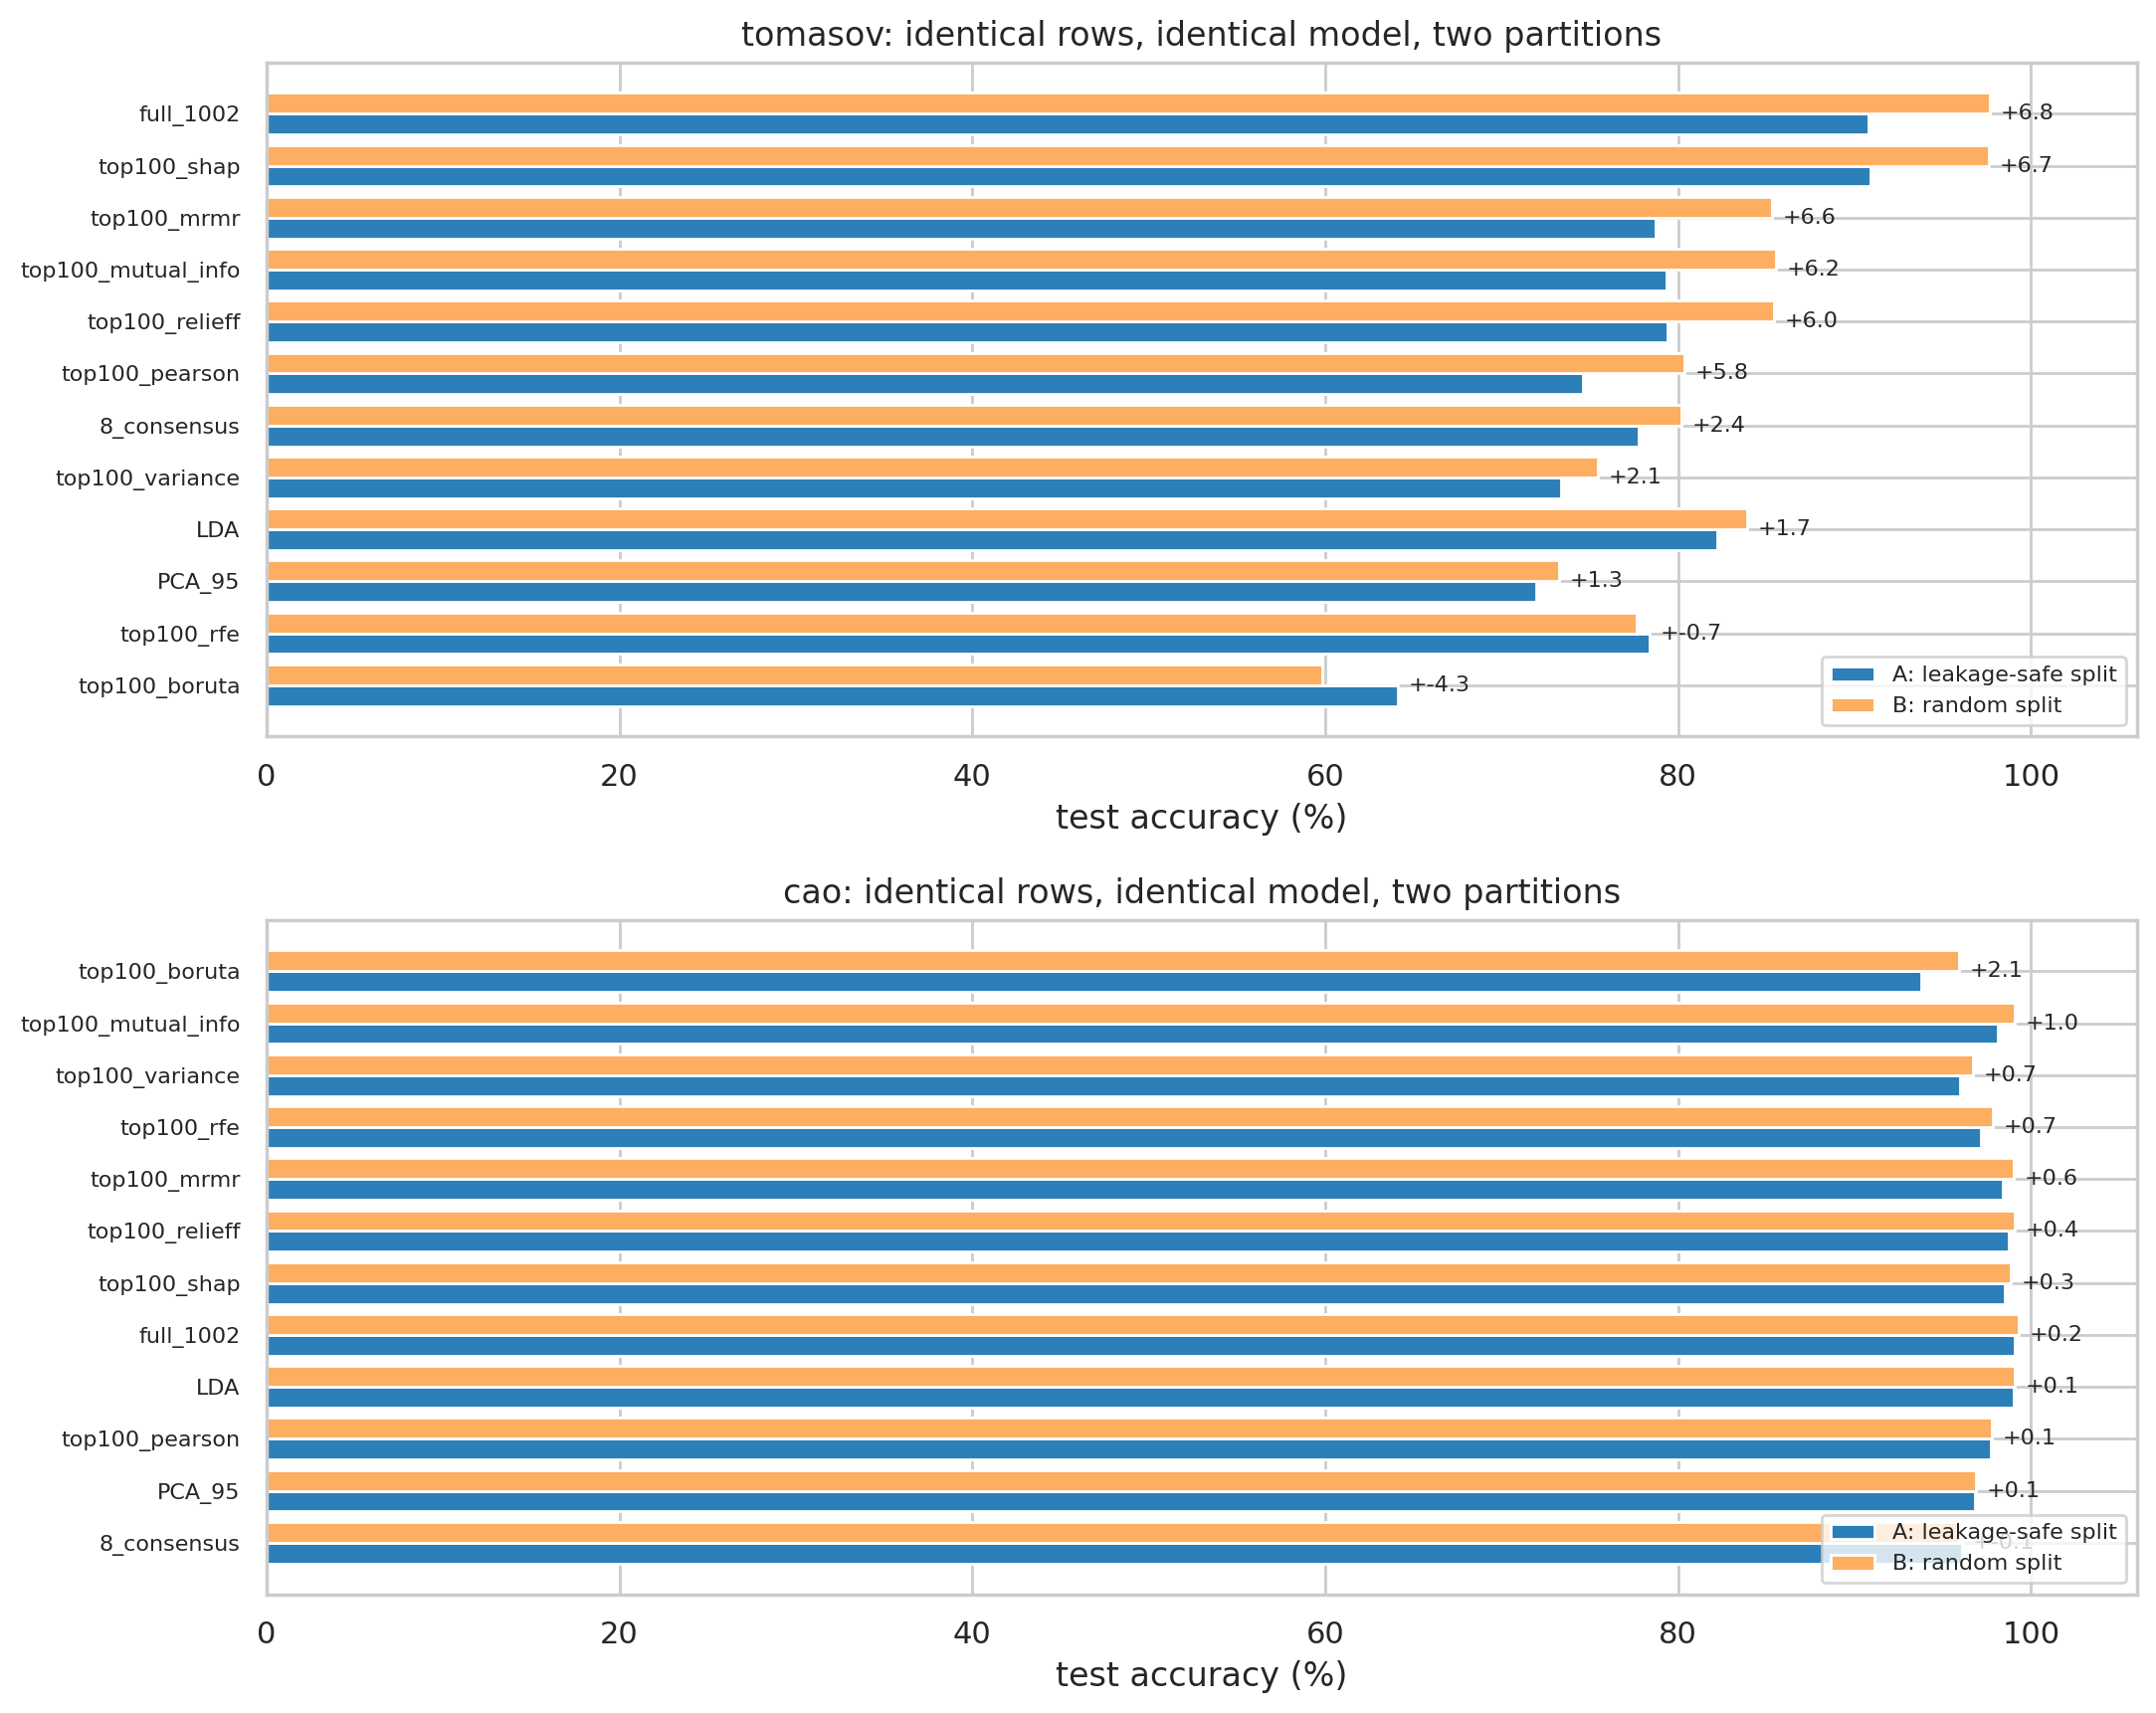
\includegraphics[width=0.88\textwidth,keepaspectratio]{Figures/fig34_protocol_inflation.png}
\caption{Protocol sensitivity of the feature pipeline: test accuracy of each feature configuration under the leakage-controlled and random partitions of the same rows, on Tomasov (top) and Cao (bottom). Annotations give the gain under the random partition.}
\label{fig:protocol_inflation}
\end{figure}

One result qualifies the overall advantage of the feature pipeline. As \refss{sec:resOpenclose} showed, no feature-based classifier recovers \emph{openclose} under leakage control ($F_1 = 0.044$ for the selected LightGBM and at most $0.189$ for any of the seven). S2-DyGNN achieves $0.625$ on the same partition and the same 198 test windows, exceeding the $0.557$ reported under its original protocol, and GCN reaches $0.433$. Models that operate directly on the channel axis thus recover a class that pooled spatial descriptors cannot distinguish.

A second qualification concerns cost, which Table~\ref{tab:sota} reports alongside the accuracies. The graph networks take preprocessed raw windows as input and compute their spectrograms within the network, so their online cost is their inference cost, $3.03$ to $5.67$\,ms per window on the GPU. DASViT1D and DAStatFormer read input features that are computed beforehand, which makes their $0.16$ to $0.76$\,ms a lower bound. The feature pipeline requires $144.59$\,ms of extraction on Tomasov and $122.54$\,ms on Cao before a classification that takes under $0.2$\,ms on the CPU. Per window and end to end, the networks are therefore faster online, and the smallest of them holds 48 thousand parameters. The lightweight advantages of the pipeline, presented in \refss{sec:resFootprint}, lie in a model a nineteenth the size of DAStatFormer and a tenth to a thirty-ninth that of the Tomasov CNN, sub-millisecond inference without a GPU, and training measured in minutes on CPU cores rather than hours on a GPU, and they are stated in those terms rather than as a lower latency.

\subsection{White-Box and Black-Box Models}
\label{sec:resWhiteBox}
\autoBookmark{subsec}{White-Box and Black-Box Models}
The preceding comparisons concern the performance of each model and its cost. This subsection addresses a different question: the extent to which a person can understand why a model reaches a given decision. It uses the distinction between white-box and black-box models introduced in \refss{sec:chap2AIMLDL}, and Table~\ref{tab:whitebox} places every model of the study on that scale. Logistic regression and the single decision tree are white boxes in the strict sense, since a weight or a threshold on a named descriptor constitutes the entire model. LightGBM, the selected learner, retains the property that is most important for audit, namely named inputs, but its $4{,}500$ trees on Tomasov are too numerous to be inspected individually. Its transparency therefore lies in its inputs, in its split structure, and in attributions that can be computed exactly for tree ensembles~\cite{lundberg2020trees}, and it is best described as a transparent ensemble over white-box features. The networks are black boxes. Their weights have no assigned meaning, and their decisions can be explained only retrospectively and only approximately~\cite{guidotti2018survey}. DAStatFormer is the closest to the pipeline, because its inputs are named statistics, but those statistics pass through 16 million weights of attention and gating layers before a decision is made.

\begin{table}[!htbp]
	\centering
	\caption{Interpretability of the models compared in this study.}
	\label{tab:whitebox}
	\footnotesize
	\setlength{\tabcolsep}{4pt}
	\renewcommand{\arraystretch}{1.15}
	\begin{tabularx}{\textwidth}{@{}>{\raggedright\arraybackslash}p{2.5cm} >{\raggedright\arraybackslash}X >{\raggedright\arraybackslash}X >{\raggedright\arraybackslash}X >{\raggedright\arraybackslash}p{1.75cm}@{}}
		\toprule
		\textbf{Model} & \textbf{Input} & \textbf{Meaning of a parameter} & \textbf{Explanation of a decision} & \textbf{Class}\\
		\midrule
		Logistic regression, decision tree & $1{,}002$ named descriptors & A weight or a threshold on one named descriptor & Read directly from the weights or the decision path & White box\\
		\addlinespace[3pt]
		LightGBM (proposed) & $1{,}002$ or 52 named descriptors, each tagged with its domain & A threshold on one named descriptor, or a leaf value & Exact Shapley attributions per window, split-based importance, and decision paths, all over named descriptors & Transparent ensemble\\
		\addlinespace[3pt]
		Tomasov and Cao CNNs & RDFT spectrum or raw record & A convolution or dense weight with no assigned meaning & Post-hoc saliency, approximate & Black box\\
		\addlinespace[3pt]
		DASViT1D & Vector of MFCC, RDFT, and DWT coefficients & A projection or attention weight & Post-hoc attention or saliency maps, approximate & Black box\\
		\addlinespace[3pt]
		DAStatFormer & 24 named statistics per channel & An attention or gating weight & Post-hoc and approximate; the inputs are named but mixed by attention & Black box\\
		\addlinespace[3pt]
		S2-DyGNN, GAT, GCN & Preprocessed multi-channel patch & A filter, graph, or attention weight; a learned channel adjacency & Post-hoc; learned edges show which channels interact, not why & Black box\\
		\bottomrule
	\end{tabularx}
\end{table}

The difference is not merely one of principle. In this thesis, interpretability enabled three analyses that would not have been possible with a black-box model. The first is the diagnosis of the spatial confound. Because every column carries its domain prefix, the representation could be decomposed domain by domain, and the leave-one-domain-out ablation and the recording-identity probe of \refs{sec:resConfound} showed that the 61 spatial descriptors both contribute $19.67$ macro-$F_1$ points and identify the source recording $11.1$ points beyond the next domain. For the networks, the same question, whether a model recognises the event or the recording, could be posed only externally, by changing the partition (\refss{sec:resReproGap}); it could not be traced to any part of the input.

The second is a comparison of the importance ranking with the definitions of the features. When the features are ranked by the frequency with which the final Tomasov model splits on them (\reff{fig:feature_importance}), five of its ten leading features, including the first three, are the Gini coefficient, maximum gradient, skewness, argmax, and kurtosis of the channel-energy profile. All five belong to the group of 29 descriptors that per-channel z-scoring makes constant in exact arithmetic (\refss{sec:chap3SpatialFeatures}). A model that relies most heavily on quantities that should carry no information is evidently using something other than the event, and the invariance audit of \refss{sec:chap5LimResidue} identified the source: a residue of approximately $10^{-14}$ left by a stabilising constant. Because each descriptor is an explicit formula, the audit could also identify the 33 descriptors that respond to changes that should not affect them. The learned features of a network have no definition against which such a check could be made.

The third is the interpretation of the selected subset. The unanimous subset is a short list of named quantities, and the five features selected on both systems, the minimum, lower quartile, and range of the STFT temporal envelope, the maximum spectral flux, and the Gini coefficient of the segment energies (\refss{sec:resConsistency}), describe how unevenly the energy of an event is distributed over the window and how abruptly its spectrum changes. An engineer can verify such statements against existing knowledge of the events, which is not possible for a learned embedding.

For perimeter security this property has practical as well as analytical value. An alert raised by the pipeline can be accompanied by the descriptors that produced it, so that an operator or an auditor can determine, for example, whether a fence alarm was based on impulsive time-domain structure or on the spatial distribution of the energy. Rudin~\cite{rudin2019stop} argues that in such high-stakes settings a model of this kind should be preferred to a black box explained retrospectively, because the explanation of a black box need not reflect the computation that the model performs. Exact attributions for tree ensembles avoid that discrepancy, since they are computed from the model itself rather than from a surrogate~\cite{lundberg2020trees}.

Interpretability is obtained at a cost, which the benchmark shows in two forms. Within the pipeline, the fully white-box learners are the weaker ones: on Tomasov the decision tree reaches $71.69$ and logistic regression $78.59$ macro-$F_1$, compared with $81.98$ for LightGBM, and on Cao $91.56$ and $97.84$ against $98.90$. The selected model therefore exchanges some transparency for accuracy. Relative to the networks, the cost is a loss of information. A designed representation retains only what its descriptors measure, and pooling over the channel axis discards the structure that enables S2-DyGNN to recover \emph{openclose} at an $F_1$ of $0.625$, whereas no feature-based learner exceeds $0.189$ (\refss{sec:resOpenclose}). The white-box design made that failure visible and explicable, but it did not prevent it. Nor has the benefit to operators been measured: the claim rests on named descriptors and attributions, and its evaluation with the personnel who act on alerts is reserved for future work (\refss{sec:chap5FutureOperators}).

On balance, the pipeline is more interpretable than the black-box networks in the sense that is relevant to audit: every input has a definition, every split refers to one of those inputs, and every attribution can be computed exactly. The same property enabled this thesis to identify, and to report, the most serious flaw in its own results.

\subsection{Overall Comparison with Published Work}
\label{sec:resSynthesis}
\autoBookmark{subsec}{Overall Comparison with Published Work}
Taken together, these comparisons explain why several results in this thesis are lower than those published for the same benchmarks. Every published Tomasov accuracy that could be re-measured under leakage control decreased: that of the reconstructed CNN from $85.47\%$ to $68.74\%$, and those of the five recent architectures by between $3.88$ and $36.35$ accuracy points, while the \emph{openclose} result of the first design cycle of this study decreased from an $F_1$ of $0.72$ to $0.044$. The controlled two-arm comparisons attribute a large proportion of these reductions to the evaluation protocol rather than to the reimplementations, since changing only the partition of otherwise identical models raises the accuracy of the reconstructed CNN by up to $26.27$ points and that of the five architectures by between $6.48$ and $18.38$ points. On Cao, whose records do not overlap, the same intervention has no consistent effect, which confines the inflation to the dataset whose windows overlap. Published figures on the Tomasov benchmark therefore cannot be compared with one another, or with leakage-controlled results, until the protocol underlying each is taken into account.

The relative standing of the methods also changes. Under their own protocols, DAStatFormer and S2-DyGNN report the highest accuracies on the Tomasov benchmark, yet under identical leakage-controlled partitions the feature pipeline exceeds them by $11.88$ and $13.12$ accuracy points, although the graph models retain their lead on \emph{openclose}. Leakage does not inflate all models equally: the low-capacity Cao CNN lost only $1.58$ accuracy points when its released partition was replaced by the session-grouped partition, whereas the graph and transformer models gained between $6.48$ and $18.38$ points from a random partition of the same Tomasov windows. Rankings obtained under contaminated protocols therefore need not agree with rankings obtained under group-aware evaluation, and for this reason every comparison in this thesis is made on identical partitions. These conclusions concern generalisation to unseen segments of represented recordings. As \refs{sec:resGeneralisationAll} and \refs{sec:resMapping} showed, performance declines further when whole recordings or acquisition campaigns are held out and collapses when a fitted model is transferred to another sensing system, regimes that none of the studies reviewed in \refs{sec:chap2RelatedWorks} evaluates.

Three of these measurements have no counterpart in the reviewed studies and constitute the principal additions of this thesis to the DAS literature: the attribution of a reproduction gap to the protocol by changing only the partition, the recording-identity probe that measures how much information each feature domain carries about the acquisition, and the transfer of a fitted model between two independent sensing systems over a mapped taxonomy. With these comparisons, \textbf{RQ3} is answered: the pipeline outperforms the published and recent baselines on identical partitions while remaining lightweight in model size, training cost, and hardware, and transparent where the networks are black boxes. It does so at a known cost in end-to-end latency, with known limits on the transferability of a fitted model, and, on Tomasov, with a margin that depends on the numerical residue of \refss{sec:chap5LimResidue}.

\section{Summary}%
\label{sec:chap4Summary}
\autoBookmark{sec}{Summary}
This chapter evaluated the artefact on the primary Tomasov dataset and the Cao evaluation dataset under a verified leakage-controlled protocol. The audit that established that protocol found that every Tomasov test window shared raw samples with a training window under a random split and that 423 of 441 Cao sessions spanned the published partition; blocked, guard-banded and session-grouped partitions reduced both measures to zero.

For \textbf{RQ1}, the footprint of every model was measured on the Jetson AGX Orin. The selected LightGBM holds $855{,}000$ parameters ($3.42$\,MB) on Tomasov and $208{,}578$ ($0.83$\,MB) on Cao, trains in $1{,}357$ and $41$\,s on CPU cores, and classifies a window in $0.17$ and $0.06$\,ms without a GPU. The model is thus a nineteenth the size of DAStatFormer and about a tenth that of the smaller Tomasov CNN, and its training requires no GPU, whereas the graph networks require seven to ten and a half hours of GPU training on Tomasov. The graph networks are smaller still and less costly end to end, because feature extraction ($122.54$--$144.59$\,ms per window) dominates the online cost of the pipeline; that cost fits within the window-arrival interval on one CPU core for Cao and two for Tomasov. The pipeline is therefore lightweight in its learning stage and its hardware requirements, and feature extraction is its most expensive component.

For \textbf{RQ2}, fusion outperformed every individual domain by $6.26$ macro-$F_1$ points on Tomasov and $3.46$ on Cao; unanimous eight-method consensus reduced the feature space by approximately $95\%$ and the training time by factors of $5.3$ to $21.5$, at a cost of $8.39$ and $5.81$ points and without reducing the size of the fitted model; and the six balancing strategies could be distinguished only modestly on Tomasov and not at all on Cao. The three gradient-boosting learners led all seven classifiers and lay within $0.62$ and $0.84$ macro-$F_1$ points of one another, and LightGBM, which validation selected in every configuration, is therefore best regarded as the representative of that tier. The pipeline designed on Tomasov was applied unchanged to Cao.

For \textbf{RQ3}, the selected configuration exceeded the CNN published with each dataset by $16.43$ and $8.01$ macro-$F_1$ points and exceeded five architectures published from 2024 onwards on identical partitions, although channel-level graph models recover \emph{openclose} where the pipeline does not. Changing only the partition altered the accuracy of an otherwise identical CNN by $26.27$ points, every recent architecture gained between $6.5$ and $18.4$ points under a random split, and removing the leakage reduced the \emph{openclose} $F_1$ of the selected model from $0.72$ to $0.044$. Unlike the black-box networks, the pipeline reaches its decisions through named descriptors, which enabled the spatial confound and the numerical residue to be traced. Generalisation beyond represented recordings is weaker. Spatial descriptors identified the source recording $11.1$ points above the next domain while contributing $19.67$ macro-$F_1$ points, two effects that this dataset cannot separate; leave-one-recording-out accuracy on Tomasov averaged $63.85\%$; holding out Cao acquisition dates reduced accuracy from $99.06\%$ to $86.81\%$; and although four event types could be mapped between the two taxonomies, a model trained on one system performed below chance on the other. Chapter~\ref{chap:Conclusion} consolidates these findings, states their novelty, and reports a numerical residue in the normalisation that qualifies the Tomasov figures.


%Chapter 5
\pagestyle{plain}\cleardoublepage%To Add an empty page and start on an odd number (SOFTBOUND)%%
\chapter{CONCLUSIONS AND FUTURE DIRECTIONS}\label{chap:Conclusion}
\autoBookmark{chap}{CONCLUSIONS AND FUTURE DIRECTIONS}
\section{Overview}%
\label{sec:chap5Overview}
\autoBookmark{sec}{Overview}
This chapter closes the DSRM cycle. It revisits each research objective against the mapping of Table~\ref{tab:dsrm_mapping}, states what is new in the work and what it contributes to knowledge, sets out the limitations, and identifies where the work should go next. Each conclusion is stated together with the scope within which it holds, because several findings of Chapter~\ref{chap:ResultsAndDiscussion} apply to recordings represented in training but not to new acquisitions or to a new sensing system.

\section{Revisiting the Research Objectives}
\label{sec:chap5Objectives}
\autoBookmark{sec}{Revisiting the Research Objectives}
An objective is regarded as met when the design, implementation, comparison, or measurement it specifies was carried out as planned and the corresponding research question can be answered from the results, whether or not the answer is the one anticipated. Where an answer differs from expectation, it is reported as measured.

\subsection{RO1: An Interpretable Pipeline Under Leakage-Controlled Evaluation}
\label{sec:chap5RO1}
\autoBookmark{subsec}{RO1: An Interpretable Pipeline Under Leakage-Controlled Evaluation}
An interpretable, feature-driven pipeline was designed on the Tomasov dataset and applied unchanged to the Cao dataset. It combines a stateless three-stage preprocessing chain, a single-pass extractor of $1{,}002$ named descriptors across the time, frequency, time--frequency, and spatial domains, and seven lightweight classifiers, and it needs no gradient-based training on the edge device. Its evaluation is part of the design. Auditing the released protocols showed that every test window of a random Tomasov split shares raw samples with a training window and that 423 of the 441 Cao sessions span both published folders. Blocked, guard-banded partitions for Tomasov and session-grouped partitions for Cao reduce both measures to zero, and their disjointness is asserted in code before any model is trained. The protocol-attribution experiments show why this matters: changing only the partition moved an otherwise identical CNN by $26.27$ accuracy points and five recent architectures by $6.5$ to $18.4$. The selected LightGBM classifies a window in under $0.2$\,ms on embedded hardware, but the lightweight claim applies to the classifier, not to the whole pipeline: extraction takes $144.59$\,ms per window on Tomasov and $122.54$\,ms on Cao, so Tomasov needs two cores to keep up with its arrival rate. The verification covers the partitions rather than the feature code, and a later audit of that code found the numerical residue reported in \refss{sec:chap5LimResidue}. RO1 is met, with that qualification.

\subsection{RO2: Multi-Domain Fusion, Feature Selection, and Class Balancing}
\label{sec:chap5RO2}
\autoBookmark{subsec}{RO2: Multi-Domain Fusion, Feature Selection, and Class Balancing}
Fusing the four domains outperformed every individual domain on both datasets, by $6.26$ macro-$F_1$ points on Tomasov and $3.46$ on Cao, so the domains carry complementary rather than redundant information. The domain ordering agreed across the two systems at $\rho = 0.90$, which points to a property of the representation rather than of one campus fibre, although the agreement weakens once the residue of \refss{sec:chap5LimResidue} is removed.

The eight-method consensus, with every selector confined to training data and refitted inside each cross-validation fold, reduced the feature space by about $95\%$, to 52 features on Tomasov and 53 on Cao. Two findings qualify this result. The reduction is not free: it costs $8.39$ and $5.81$ macro-$F_1$ points, far more than the sub-point penalty reported in earlier single-dataset work, so an intermediate operating point on the reduction curve is preferable unless inference cost or interpretability dominates. And the six balancing strategies separated only modestly on Tomasov and not at all on Cao when compared over independent held-out acquisitions, so the expectation that cost-sensitive weighting would be consistently superior was not supported. RO2 is met, with both qualifications reported as measured.

\subsection{RO3: Comparative Performance, Cost, and Generalisation}
\label{sec:chap5RO3}
\autoBookmark{subsec}{RO3: Comparative Performance, Cost, and Generalisation}
Seven classifiers were benchmarked across six balancing strategies on both datasets. The three gradient-boosting learners led on both and lay within $0.62$ and $0.84$ macro-$F_1$ points of one another, so LightGBM, which validation selected in every configuration, is best regarded as the representative of that tier rather than as a learner shown to beat the other two. It reached $90.71\%$ accuracy and $81.98$ macro-$F_1$ on Tomasov and $99.06\%$ and $98.90$ on Cao, and its lead over random forest and logistic regression held on all five independently generated partitions.

Against the CNN published with each dataset, reimplemented from the released code or the paper's specification and trained on identical partitions, the pipeline led by $16.43$ and $8.01$ macro-$F_1$ points; the Tomasov reconstruction exceeds its own published figure under the original protocol, so it is not a weakened comparator. Against five architectures published from 2024 onwards, trained under the same partitions, the pipeline led the strongest neural baseline by $11.88$ accuracy points on Tomasov and $1.11$ on Cao. With the residue of \refss{sec:chap5LimResidue} removed, the Tomasov lead narrows to $1.69$ points and S2-DyGNN moves ahead on macro-$F_1$. The neural baselines, which consume raw windows, are nevertheless between twenty and nine hundred times cheaper online, so the pipeline's advantages are interpretability and training cost rather than latency.

Generalisation was tested under progressively stricter protocols. Accuracy averaged $63.85\%$ (SD $29.31$) on unseen recordings of the four Tomasov classes recorded more than once, and fell from $99.06\%$ to $86.81\%$ on unseen Cao acquisition dates. Mapping the two taxonomies onto four shared event types showed that these events are recognised well within each system ($73.02\%$ and $95.93\%$ accuracy from non-spatial features) but that a model trained on one system scores below chance on the other ($14.41\%$ and $19.12\%$). Repeating the leakage-controlled partition with five seeds gave a Tomasov standard deviation of $4.42$ macro-$F_1$ points, so every headline figure on that dataset carries a substantial partition uncertainty. RO3 is met: the comparisons and cost measurements were made as planned, and the generalisation limits are reported as found.

\section{Contributions to Knowledge}
\label{sec:chap5Contributions}
\autoBookmark{sec}{Contributions to Knowledge}
The novelty of this thesis does not lie in a new learning algorithm. Gradient boosting, wavelet descriptors, SMOTE, and blocked cross-validation are all established. What is new, seen from information technology and computer science, is a way of building and measuring a DAS classifier in which the validity of the evaluation is a tested property of the software. Provenance is recorded before any signal is read, a partition that fails its checks stops the run, each claim about a model is tied to a controlled experiment that changes one factor, and cost is measured for the whole pipeline rather than for the classifier alone.

In the knowledge-contribution framework of Gregor and Hevner~\cite{gregor2013positioning}, the evaluation protocol is an \emph{exaptation}: blocked and group-aware evaluation are known solutions from other fields, carried here into a field that had not applied them. The attribution design, the recording-identity probe, the invariance audit, and the feature pipeline are \emph{improvements}, new solutions to a known problem. No claim of invention is made. Table~\ref{tab:novelty_evidence} sets each element introduced in \refss{sec:ThesisNovelty} beside the evidence for it.

\begin{table}[!htbp]
	\centering
	\caption[Novel elements of the thesis and the evidence for each]{Novel elements of the thesis, the kind of knowledge contribution each makes in the framework of Gregor and Hevner~\cite{gregor2013positioning}, and the measured evidence for each.}
	\label{tab:novelty_evidence}
	\footnotesize
	\setlength{\tabcolsep}{4pt}
	\renewcommand{\arraystretch}{1.2}
	\begin{tabularx}{\textwidth}{@{}>{\raggedright\arraybackslash}p{4.1cm} >{\raggedright\arraybackslash}p{1.9cm} >{\raggedright\arraybackslash}X@{}}
		\toprule
		\textbf{Novel element} & \textbf{Type} & \textbf{Evidence in this thesis}\\
		\midrule
		Evaluation validity asserted in code, with provenance manifests & Exaptation & Test windows sharing raw samples with training fall from $100\%$ to $0\%$ on Tomasov; sessions spanning the split fall from 423 of 441 to none on Cao.\\
		\addlinespace[3pt]
		Blocked partitioning with guard bands derived from read footprints & Exaptation & All nine classes stay in every split, including the five single-recording classes, at a cost of $9.00\%$ of the annotated windows.\\
		\addlinespace[3pt]
		Protocol-attribution experiments & Improvement & Changing only the partition moves an identical CNN by $26.27$ accuracy points and five recent architectures by $6.48$ to $18.38$.\\
		\addlinespace[3pt]
		Recording-identity probe & Improvement & Spatial descriptors identify the source recording $11.1$ points beyond the next domain, yet removing them costs $19.08$ accuracy points on unseen recordings.\\
		\addlinespace[3pt]
		Four-domain representation with unanimous consensus selection & Improvement & Fusion leads the best single domain by $6.26$ and $3.46$ macro-$F_1$ points; consensus removes about $95\%$ of the features at a cost of $8.39$ and $5.81$.\\
		\addlinespace[3pt]
		Whole-pipeline cost accounting on embedded hardware & Improvement & On Tomasov, extraction takes $144.59$\,ms and inference $0.17$\,ms against a $102.4$\,ms window interval, so extraction sets the real-time budget.\\
		\addlinespace[3pt]
		Mechanism-based taxonomy mapping and cross-system transfer test & Exaptation & Four shared events are recognised at $73.02\%$ and $95.93\%$ accuracy within each system but at $14.41\%$ and $19.12\%$ across systems, below the $25\%$ chance level.\\
		\addlinespace[3pt]
		Invariance audit of the feature code & Improvement & Thirty-three of the $1{,}002$ descriptors respond to changes that should not reach them, and the residue accounts for about ten Tomasov accuracy points (\refss{sec:chap5LimResidue}).\\
		\bottomrule
	\end{tabularx}
\end{table}

These elements yield six findings that matter for DAS research more broadly.

The first is that the evaluation protocol, not the architecture alone, governs the headline results on this benchmark. Holding a model fixed and changing only the partition altered its accuracy by $26.27$ points, and the same intervention changed five recent architectures by $6.5$ to $18.4$ points. Published accuracies obtained under random or chronological partitions of overlapping windows are therefore not directly comparable and should not be read as model rankings.

The second is that leakage substantially inflated minority-class performance, while the feature representation remained the limiting factor. Once contamination was removed, the \emph{openclose} class fell from a published $F_1$ of $0.72$ to $0.044$ for the selected model, and none of the seven classifiers exceeded $0.19$. The class is not unlearnable from the data: on the same partition and the same 198 test windows, S2-DyGNN reaches $0.625$, GCN $0.433$, and GAT $0.278$, each above every feature-based classifier. It is the pooled descriptors used here, whose 61 spatial features aggregate across the channel axis, that cannot recover it. Because \emph{openclose} corresponds to unauthorised manhole access, the correction matters operationally, and it identifies a case in which pooled descriptors should be replaced or supplemented by a model that keeps the channel axis.

The third is that a feature set can be informative and confounded at the same time. In the recording-identity probe, spatial descriptors identified the source recording with a margin $11.1$ points larger than that of the next domain, yet leave-one-recording-out evaluation showed that removing them reduced cross-recording accuracy by $19.08$ points. Both findings hold, and they cannot be separated in a dataset in which five of the nine classes come from a single recording. The methodological contribution is the probe itself, a diagnostic that quantifies the confound rather than presuming it absent.

The fourth is that statistics must be computed over independent acquisitions. The Friedman test, applied with balancing strategies as blocks, returned a near-maximal statistic that reflected the dependence between blocks rather than an effect, and it was withdrawn. Repeating the partition with five seeds gave a Tomasov standard deviation of $4.42$ macro-$F_1$ points, and bootstrapping over recordings rather than windows widened the confidence interval by an order of magnitude. Any headline figure on a dataset with few independent recordings must carry that uncertainty.

The fifth is that a method can generalise across sensing systems while a fitted model does not. The same pipeline configuration, untuned, recognised the shared event types within each of two unrelated systems, yet a model fitted on one system and applied to the other, on four carefully mapped event types, scored below chance in both directions. Cross-system claims in DAS should therefore state which of the two is meant, and the mapping between the Tomasov and Cao taxonomies gives future adaptation methods a concrete benchmark on which to show progress.

The sixth concerns leakage below the level of the partition. A constant of $10^{-12}$ added to a denominator for numerical safety left about $10^{-14}$ of each channel's raw amplitude in the features, and tree ensembles, which compare values rather than weigh them, could split on it (\refss{sec:chap5LimResidue}). No partition check can see such a path, because it runs through the feature code rather than through the split. A simple invariance audit can: multiply each raw channel by its own gain and test which features move. Any pipeline that claims amplitude normalisation, in DAS or elsewhere, can run this check on a few windows per recording, and the audit is released with this thesis.

\section{Limitations}
\label{sec:chap5Limitations}
\autoBookmark{sec}{Limitations}
The conclusions above hold within limits, set out here as threats to validity. \refss{sec:chap5LimConfound} and \refss{sec:chap5LimResidue} concern internal validity, whether measured performance reflects the event rather than the recording, and they bear most directly on the headline figures. \refss{sec:chap5LimMethod} concerns the strength of the comparisons, and \refss{sec:chap5LimScope} concerns external validity, how far the findings extend beyond these datasets and this offline setting.

\subsection{The Recording Confound Cannot Be Resolved with These Datasets}
\label{sec:chap5LimConfound}
\autoBookmark{subsec}{The Recording Confound Cannot Be Resolved with These Datasets}
The central structural limitation lies in the data. Because five Tomasov classes each come from a single recording, recording identity and class identity are indistinguishable for them, and no partition can separate their effects. Two operating points are therefore reported, but definitive attribution needs a dataset with several independent recordings per class. The Tomasov probe also rests on limited evidence: after degenerate cases are excluded, only one class remains suitable for analysis, so that measurement should be regarded as indicative. Five probes remain valid on Cao, which gives stronger evidence of a dataset-wide campaign confound. The Tomasov labels themselves were drawn by hand on band-limited power maps, and their noise was not estimated.

\subsection{A Numerical Residue in Amplitude Normalisation}
\label{sec:chap5LimResidue}
\autoBookmark{subsec}{A Numerical Residue in Amplitude Normalisation}
The z-score of \refss{sec:chap3Normalisation} was implemented with the customary stabilising constant, dividing by $\sigma_{\mathcal{H}} + \epsilon$ with $\epsilon = 10^{-12}$. After the experiments of Chapter~\ref{chap:ResultsAndDiscussion} had been completed, an invariance audit tested the feature code directly: each raw channel was multiplied by its own gain between $0.25$ and $4$, each raw sample was perturbed by about one part in $10^{12}$, and every descriptor was compared before and after. Per-channel z-scoring should make all $1{,}002$ descriptors indifferent to such changes. Thirty-three were not: thirteen carried each channel's raw amplitude through the constant, and the rest followed floating-point rounding. A channel with standard deviation $\sigma_c$ ends up with energy $T(1 - 2\epsilon/\sigma_c)$ rather than exactly $T$, an imprint of about $10^{-14}$. That is far below any physical scale and close to the limit of double-precision arithmetic~\cite{goldberg1991floating}, but a decision tree compares values rather than weighing them and can place a split between any two distinct numbers. The residue therefore reopens, in numerical form, the fingerprint of gain and coupling that normalisation is meant to close. The partition checks cannot detect it, since it involves no shared samples.

Chapter~\ref{chap:ResultsAndDiscussion} reports the experiments as executed, with the constant in place. Table~\ref{tab:residue_effect} sets those figures beside the same measurements with the chain made exact: dividing by $\sigma_{\mathcal{H}}$ alone, writing the descriptors that are constant by construction as exact constants, and flooring the spectrum at $-120$\,dB.

\begin{table}[!htbp]
	\centering
	\caption{Effect of the numerical residue: the figures reported in Chapter~\ref{chap:ResultsAndDiscussion}, with the constant in place, beside the same measurements with the chain made exact.}
	\label{tab:residue_effect}
	\small
	\setlength{\tabcolsep}{4pt}
	\begin{tabular}{@{}lrr@{}}
		\toprule
		\textbf{Measure} & \textbf{As reported} & \textbf{Exact chain}\\
		\midrule
		\multicolumn{3}{@{}l}{\textit{Tomasov}}\\[2pt]
		Accuracy of the selected model (\%)                    & 90.71 & 80.52\\
		Macro-$F_1$ of the selected model                      & 81.98 & 76.33\\
		\emph{Openclose} $F_1$ of the selected model           & 0.044 & 0.263\\
		Macro-$F_1$ without the spatial block                  & 62.13 & 62.07\\
		Macro-$F_1$ lost on removing the spatial block         & 19.67 & 14.84\\
		Spatial recording identification above chance (points) & 12.9  & 8.8\\
		Leave-one-recording-out accuracy (\%)                  & 63.85 & 53.81\\
		Macro-$F_1$ over five partitions (mean $\pm$ SD)       & $80.47 \pm 4.42$ & $73.04 \pm 3.22$\\
		\midrule
		\multicolumn{3}{@{}l}{\textit{Cao}}\\[2pt]
		Accuracy of the selected model (\%)                    & 99.06 & 98.50\\
		Macro-$F_1$ of the selected model                      & 98.90 & 98.18\\
		Leave-one-date-out accuracy (\%)                       & 86.81 & 85.98\\
		\midrule
		\multicolumn{3}{@{}l}{\textit{Across the two systems}}\\[2pt]
		Transfer accuracy, Cao to Tomasov (\%)                 & 14.41 & 15.76\\
		Transfer accuracy, Tomasov to Cao (\%)                 & 19.12 & 20.25\\
		Rank correlation of the feature domains ($\rho$)       & 0.90  & 0.50\\
		\bottomrule
	\end{tabular}
\end{table}

The effect is large on Tomasov and small on Cao. Tomasov accuracy falls by $10.19$ points to $80.52\%$ and macro-$F_1$ by $5.65$ to $76.33$, with XGBoost rather than LightGBM as the validated choice, which is no surprise given that the boosted learners cannot be separated (\refss{sec:resAllModels}). Cao moves by $0.56$ and $0.72$. The Tomasov headline of Chapter~\ref{chap:ResultsAndDiscussion} should therefore be read as an upper bound, with about ten of its accuracy points owed to the residue rather than to the events.

Several conclusions change in degree. The lead over the published Tomasov CNN falls from $16.43$ to $10.78$ macro-$F_1$ points. The lead over the strongest neural baseline falls from $11.88$ to $1.69$ accuracy points, and on macro-$F_1$ the $78.54$ of S2-DyGNN moves ahead of $76.33$. The residue sits in the channel-energy descriptors, so the contribution of the spatial domain and its recording-identity margin both shrink, and the fall of that domain on Cao lowers the agreement between the two systems from $\rho = 0.90$ to $0.50$. Cross-recording accuracy drops by a further ten points.

Others hold. Neither the leakage audit, nor the partitions, nor any neural baseline reads these features, so the protocol-attribution results of \refs{sec:resDiscussion} are untouched. Fusion still leads the best single domain on both datasets, by $6.22$ and $5.84$ macro-$F_1$ points. The spatial domain remains the strongest single domain on Tomasov, and the conservative no-spatial figure of \refss{sec:resConfoundVerdict} barely moves. \emph{Openclose} stays below all three graph models, and cross-system transfer stays below chance.

\subsection{Methodological Scope}
\label{sec:chap5LimMethod}
\autoBookmark{subsec}{Methodological Scope}
Several comparisons rest on single runs or on choices that were fixed rather than optimised. Each CNN and neural baseline was trained once, at one seed. On a class of 198 test windows a single run is a weak estimate, so the \emph{openclose} values of Table~\ref{tab:sota} show that the class carries signal a channel-level model can use, not what these models reach reliably, and the conclusion rests on the pattern across the three graph models rather than on the $0.625$ of S2-DyGNN alone. The classical learners share one hyperparameter configuration, which keeps the comparison fair between them but does not establish the best each could reach. In the consensus ensemble, mRMR scores 400 features while the retention rule keeps 501, so 101 of its votes fall to tie-breaking. Some features therefore leave the unanimous subset for reasons unconnected with their merit, and the reported subset is probably smaller, and its cost larger, than a full ranking would give.

The baselines are reconstructions. Where a recent architecture's publication left a detail unstated, the choice made is recorded rather than tuned, so those baselines are faithful reconstructions rather than the authors' own code. Because librosa was not usable on the embedded platform, the MFCC branch of DASViT1D uses a SciPy implementation that yields 980 values rather than the $1{,}300$ of the librosa configuration, so its results are specific to that front end. The RDFT redundancy factor for the Tomasov CNN was inferred from two stated quantities rather than read directly, and only the RDFT front end was evaluated, not the MFCC and DWT variants the same publication reports. The re-cut partition used for protocol attribution reconstructs the published protocol rather than reproducing it, and single-run CNN accuracies on Tomasov vary by a few tenths with row ordering alone. The Cao sampling rate is a nominal value because the release does not identify which fibre span produced each record, and the Cao CNN was not evaluated under leave-one-date-out, so the capacity-versus-leakage observation is established for within-campaign evaluation only. Finally, the verification code is written for the metadata of these two datasets, and applying it elsewhere needs engineering effort.

\subsection{Deployment Scope}
\label{sec:chap5LimScope}
\autoBookmark{subsec}{Deployment Scope}
Within the scope of these datasets, a fitted model should be regarded as valid only for the acquisition campaign and the interrogator that produced its training data. The two datasets differ in almost every respect: Tomasov has nine classes from 16 phase-sensitive recordings over $1{,}700$ loci, and Cao six classes from 441 intensity-based sessions over 12 channels, with different sampling, geometry, labels, and sample units. Applying one pipeline to both shows that the method carries over, but the cross-system transfer test shows that a fitted model does not. That test covers only the four event types with a one-to-one counterpart, and those correspondences are approximate: construction machinery and manual digging, or a fence strike and a knock on the ground, excite the fibre differently. Robustness to weather, seasonal variation, soil properties, burial depth, source direction relative to the fibre, and other interrogator hardware was not evaluated.

The evaluation was also offline. Every result comes from stored recordings; the pipeline has not been connected to a live interrogator, and its energy draw was not measured. The real-time budget of Table~\ref{tab:efficiency} concerns one stream of windows at one locus, whereas an interrogator reports $1{,}700$ loci. The Tomasov test set is decimated in the same proportion as the training set, so its accuracy and error rates do not reflect the prevalence of routine activity on a live fibre, where \emph{regular} would dominate and false alarms would weigh more heavily. Interpretability, finally, is argued from named descriptors and attribution scores; it has not been tested with the operators who would act on the alerts.

\section{Future Directions}
\label{sec:chap5Future}
\autoBookmark{sec}{Future Directions}
The limitations point to seven directions, presented in order of expected value (Table~\ref{tab:limits_future}). The first three strengthen the evidence and make it reusable, the next two improve the model, and the last two move the artefact towards use. Each builds directly on an artefact or finding of this thesis rather than requiring it to be rebuilt.

\begin{table}[!htbp]
	\centering
	\caption{From limitations to future work.}
	\label{tab:limits_future}
	\footnotesize
	\setlength{\tabcolsep}{4pt}
	\renewcommand{\arraystretch}{1.2}
	\begin{tabularx}{\textwidth}{@{}>{\raggedright\arraybackslash}X >{\raggedright\arraybackslash}X >{\raggedright\arraybackslash}p{1.6cm}@{}}
		\toprule
		\textbf{Limitation} & \textbf{Direction} & \textbf{Subsection}\\
		\midrule
		Numerical residue in the reported figures; single training runs for the baselines & Re-baseline with exact normalisation and repeated training & \ref{sec:chap5FutureBaseline}\\
		\addlinespace[3pt]
		Recording and class cannot be separated for five Tomasov classes & Collect a dataset with several recordings per class & \ref{sec:chap5FutureDataset}\\
		\addlinespace[3pt]
		Verification code written for two datasets & Package the controls as reusable software & \ref{sec:chap5FutureTooling}\\
		\addlinespace[3pt]
		Pooled descriptors cannot recover \emph{openclose} & Combine them with a channel-level model & \ref{sec:chap5FutureChannelModel}\\
		\addlinespace[3pt]
		Fitted models fail on unseen recordings, campaigns, and systems & Pursue domain adaptation & \ref{sec:chap5FutureAdaptation}\\
		\addlinespace[3pt]
		Extraction exceeds the Tomasov window interval; evaluation is offline and at one locus & Reduce extraction cost and move to streaming deployment & \ref{sec:chap5FutureCost}\\
		\addlinespace[3pt]
		Interpretability argued but not tested with users & Evaluate interpretability with operators & \ref{sec:chap5FutureOperators}\\
		\bottomrule
	\end{tabularx}
\end{table}

\subsection{Re-Baseline the Benchmark}
\label{sec:chap5FutureBaseline}
\autoBookmark{subsec}{Re-Baseline the Benchmark}
The first step is inexpensive. Every table of Chapter~\ref{chap:ResultsAndDiscussion} should be regenerated with the exact chain of Table~\ref{tab:residue_effect}, and the CNNs and neural baselines should be trained over several seeds, so that per-class values, \emph{openclose} above all, carry an interval rather than a point. The invariance audit should then run as a standing gate beside the partition checks, so that a later change to the feature code cannot reopen the same path unnoticed.

\subsection{Collect a Multi-Recording Dataset}
\label{sec:chap5FutureDataset}
\autoBookmark{subsec}{Collect a Multi-Recording Dataset}
Repeating each event class across separate fibre sections, days, and coupling conditions would allow the recording confound to be resolved rather than merely measured, and would permit leave-one-recording-out evaluation for the full taxonomy. This is the most valuable new evidence for this benchmark. Such a dataset would also let the recording-identity probe be applied to every class rather than to the single Tomasov class that survives its exclusion criteria, and the partition and verification procedures developed here could be applied to it unchanged.

\subsection{Package the Leakage Controls as Reusable Software}
\label{sec:chap5FutureTooling}
\autoBookmark{subsec}{Package the Leakage Controls as Reusable Software}
The manifests, the partition assertions, the attribution harness, and the invariance audit are written for two datasets. Generalised into an installable library, driven by a declarative description of a dataset's dependence groups, they could run as an automated test in any DAS project, much as continuous integration runs unit tests, and fail a build when a split shares samples. Frozen public manifests could then support a shared leaderboard on which results are comparable because their protocol is the same. Software-engineering work on machine-learning systems has argued for this kind of automated readiness testing~\cite{sculley2015debt,breck2017mltest}, and DAS benchmarks are an open place to apply it.

\subsection{Combine Pooled Descriptors with a Channel-Level Model}
\label{sec:chap5FutureChannelModel}
\autoBookmark{subsec}{Combine Pooled Descriptors with a Channel-Level Model}
The \emph{openclose} result shows that graph models operating over the channel axis recover information that aggregate spatial descriptors lose, while the feature pipeline is stronger on the other classes. A natural extension would add a graph model's channel-level embedding to the engineered feature space, or route low-confidence windows to the graph model. Because the two approaches fail in different places, such a hybrid could keep the interpretability of the descriptors for the classes they handle well while delegating the channel-dependent class to a model that preserves the channel axis.

\subsection{Pursue Domain Adaptation Rather than Further Feature Engineering}
\label{sec:chap5FutureAdaptation}
\autoBookmark{subsec}{Pursue Domain Adaptation Rather than Further Feature Engineering}
A twelve-point fall from within-campaign to cross-campaign accuracy on Cao, a twenty-seven-point fall to unseen recordings on Tomasov, and below-chance transfer between the two systems all point to distribution shift as the binding constraint on deployment. Transfer learning, domain-adversarial training, explicit calibration, and open-set detection of unseen events are the appropriate responses. The leave-one-date-out and leave-one-recording-out protocols of this thesis, together with the four-class mapping between the Tomasov and Cao taxonomies, provide an evaluation framework against which such methods can be measured without reintroducing leakage.

\subsection{Reduce Extraction Cost and Move to Streaming Deployment}
\label{sec:chap5FutureCost}
\autoBookmark{subsec}{Reduce Extraction Cost and Move to Streaming Deployment}
Feature extraction, not inference, sets the real-time budget, and the time--frequency domain accounts for about $60$\,ms per window. GPU-accelerated wavelet-packet decomposition, or removing texture descriptors that the consensus subsets rarely retain, would improve deployability more than further classifier tuning. Because the consensus subsets keep only 52 to 53 of the $1{,}002$ features, extracting only those descriptors would cut the per-window cost further, at the accuracy cost quantified in \refs{sec:resSelection}.

Lower cost per window is only the first requirement, because the pipeline has yet to meet a live stream. A deployment study would connect it to an interrogator through a streaming ingest layer, process many loci concurrently, and measure throughput, end-to-end latency, memory, and energy draw on the embedded platform, the quantities an integrator needs and this thesis does not report. Integration with alarm-management software would then allow a nuisance-alarm budget to be evaluated at natural class prevalence.

\subsection{Evaluate Interpretability with Operators}
\label{sec:chap5FutureOperators}
\autoBookmark{subsec}{Evaluate Interpretability with Operators}
The claim of interpretability rests on named descriptors and attribution scores. Whether these help a security operator decide faster, or trust an alert more appropriately, is an empirical question for a user study that compares alerts with and without feature-level explanations. Such a study would also show which descriptors, or which summaries of them, mean something to the people who act on them.

\section{Concluding Remarks}
\label{sec:chap5Closing}
\autoBookmark{sec}{Concluding Remarks}
This thesis set out to build an accurate, interpretable, and deployable DAS event classifier, and to measure it in a way that others can check. Multi-domain handcrafted features paired with gradient boosting, designed on the Tomasov perimeter-security dataset and applied unchanged to the Cao dataset, outperform the convolutional network published with each dataset and five recent transformer and graph architectures on identical leakage-controlled partitions, with sub-millisecond inference on embedded hardware. That result holds for unseen segments of represented recordings, and it comes with an explicit account of where the artefact falls short: a numerical residue in the normalisation that flatters the Tomasov figures and narrows the lead over the neural baselines, a minority class that only channel-level models recover, a real-time budget set by feature extraction rather than inference, a substantial fall in accuracy when whole recordings or acquisition campaigns are held out, and no transfer of a fitted model between sensing systems.

The more durable contribution concerns how such systems are measured. Two widely used public benchmarks were shown to permit substantial information leakage, and correcting it changed not only the headline figures but the qualitative conclusions. A minority class believed detectable proved unrecoverable from pooled descriptors by any of seven classifiers; a balancing strategy believed superior proved hard to distinguish from its alternatives; a feature domain believed to encode event physics proved to encode acquisition identity as well; and the ordering of published architectures did not survive evaluation under one protocol. None of these corrections required a new algorithm. They required an evaluation protocol that could be verified, and statistics computed over genuinely independent units. Turned on the thesis's own feature code, the same discipline found the residue that qualifies its headline.

Group-aware, cross-campaign evaluation should therefore become standard practice in DAS event classification. Without it, published accuracies cannot be compared with one another and do not predict what a deployed system will do. The partition manifests, verification code, protocol-attribution design, and cross-dataset label mapping released with this thesis are intended to make that practice straightforward to adopt on the two public benchmarks examined here.



\clearpage
%6. Bibliography
\addtocontents{toc}{\protect\setcounter{tocdepth}{1}}
\addcontentsline{toc}{section}{\hspace*{-\cftsecindent}REFERENCES}
\label{chap:REFERENCES}
\pdfbookmark[1]{REFERENCES}{chap:REFERENCES} 


\begin{singlespace}
% \setstretch{0.8}
\setlength\bibitemsep{8pt}   % length between two different entries: original is 8pt edited by SAF1
	% \scriptsize
	% \raggedright
	% \bibliographystyle{unsrt}
	% \bibliography{refs}
	\printbibliography[title={\normalsize\normalfont\centering{REFERENCES}}]%<options>]
\end{singlespace}
\clearpage


%Grant
\phantomsection%
\addcontentsline{toc}{chapter}{\hspace*{-\cftsecindent}LIST OF RESEARCH GRANTS}
\chapter*{ \normalsize \centerline{LIST OF RESEARCH GRANTS}}
\label{chap:RESEARCHGRANT}
\pdfbookmark[1]{LIST OF RESEARCH GRANT}{chap:RESEARCHGRANT} 
\begin{enumerate}[label=\arabic*.]
    \item Data Analytics and Visualization Development System for Subsurface CO$_2$ Storage and Fluid Production.
\end{enumerate}  % Uncomment This line


%Publications
\phantomsection%
\addcontentsline{toc}{chapter}{\hspace*{-\cftsecindent}LIST OF PUBLICATIONS}
\chapter*{ \normalsize \centerline{LIST OF PUBLICATIONS}}
\label{chap:listOfPublications}
\pdfbookmark[1]{LIST OF PUBLICATIONS}{chap:listOfPublications} 
\begin{enumerate}[label=\arabic*.]
    \justifying

    \item \textbf{Khan, R. A.}, Shuhidan, S. M., Aziz, I. A., Shahabudin, M. S., and Paputungan, I. V. (2026). \textit{Event Classification in Distributed Acoustic Sensing Data: Multi-Representation Feature Engineering with Leakage-Controlled Benchmarking}. International Journal of Intelligent Engineering and Systems (IJIES). Published. \\ \textbf{[Journal]}

    \item \textbf{Khan, R. A.}, Shuhidan, S. M., and Paputungan, I. V. (2025). \textit{Framework for Real-Time Anomaly Detection in Carbon Capture and Storage using Distributed Acoustic Sensing Data}. 2025 IEEE Asia-Pacific Conference on Geoscience, Electronics and Remote Sensing Technology (AGERS). \\ \textbf{[Conference]}

\end{enumerate}



% % Appendices
% \pagestyle{plain}\cleardoublepage %To add an empty page and start on an odd number (SOFTBOUND)%%
% \appendix
% % The following 2 lines add the word appendices to the toc and prevent appendix chapters from appearing
% \addtocontents{toc}{\protect\setcounter{tocdepth}{-1}} \addtocontents{toc}{\protect\setcounter{tocdepth}{0}}
% \addcontentsline{toc}{section}{\hspace*{-\cftsecindent}APPENDICES} \addtocontents{toc}{\protect\setcounter{tocdepth}{-1}}
% \label{chap:app}
% \pdfbookmark[1]{APPENDICES}{chap:app} 

% % \pagestyle{plain}\cleardoublepage %To Add an empty page and start on an odd number (SOFTBOUND)%%
\appendix
\renewcommand{\thesection}{\Roman{section}}
% Add the appendices heading to the table of contents.
\phantomsection%
\addcontentsline{toc}{chapter}{\hspace*{-\cftsecindent}APPENDICES}
\label{chap:app}%

% \renewcommand{\chapter}{Appendix}
% \addtocontents{toc}{\protect\setcounter{tocdepth}{1}}
% \addcontentsline{toc}{section}{\hspace*{-\cftsecindent}APPENDIX A: SUPPLEMENTARY RESULTS}
% \chapter{SUPPLEMENTARY RESULTS: GENERALIZATION ACROSS DATASETS}
% \label{app:results}
% \pdfbookmark[2]{APPENDIX A}{app:results} 
% \input{Chapters/appResults}

% \addtocontents{toc}{\protect\setcounter{tocdepth}{1}}
% \addcontentsline{toc}{section}{\hspace*{-\cftsecindent}APPENDIX B: IMPLEMENTATION}
\chapter{CODE AND DATA AVAILABILITY}
\label{app:implementation}
\pdfbookmark[2]{APPENDIX B}{app:implementation} 
This appendix identifies the location and contents of the implementation, partition manifests, and result artefacts used in the experiments. They are released so that every result reported in Chapter~\ref{chap:ResultsAndDiscussion} can be audited on the identical partitions, and so that other researchers can evaluate their own models on the two public benchmarks without the contamination present in the released protocols.

\section{Code and Result Artefacts}
\label{sec:codeAvailability}
The code used to conduct the experiments is publicly available in the repository \href{https://github.com/reeyan-afzal-khan/THESIS-MASTERS-UTP}{THESIS-MASTERS-UTP}. It is organised as a shared Python library (\texttt{dasfe}) and a numbered notebook series that orchestrates it, from environment setup and dataset inventory through leakage assessment, partitioning, feature extraction, fusion, selection, benchmarking, cross-dataset generalisation with the Tomasov--Cao label mapping, the CNN and recent-architecture baselines, the spatial-confound ablation, repeated-partition and bootstrap statistics, protocol attribution, and the head-to-head comparison with recent architectures.

The frozen partition of each dataset is released as a manifest keyed by sample identifier, which records each window's presence before guard-band removal, after guard-band removal, and after decimation (\refss{sec:chap3Implementation}). Every experiment reads its split membership from this manifest rather than re-deriving it. The per-experiment predictions, full-precision metrics, experiment registry, the assumption files recorded for each reimplemented baseline, and a deterministic script that regenerates the reported tables are stored alongside the code.

The stored results are those reported in Chapter~\ref{chap:ResultsAndDiscussion}. The released library also contains the exact normalisation and the invariance audit of \refss{sec:chap5LimResidue}, so executing it yields the corrected figures of Table~\ref{tab:residue_effect}.



\end{document}